\chapter{Alignement et \'etude du bruit de fond faisceau \`a l'ILC}
\label{chap:alignement}

\section{Introduction}

  L'alignement constitue la premi\`ere \'etape du processus de prise de donn\'ees. Pour pouvoir utiliser un détecteur, il est nécessaire d'aligner chaque composante du détecteur avec une précision supérieure à sa résolution intrinsèque. Un alignement dit "nominal" de chaque sous-partie du détecteur de l'ordre de la centaine de microns est possible. Cet alignement se base sur la mesure de chaque \'el\'ement d'un d\'etecteur lors de la construction et sur un syst\`eme de mesures optiques par la suite. Cependant, cette précision n'est pas suffisante pour un détecteur de vertex qui vise une résolution spatiale de seulement quelques microns. Pour l’ILC, afin de s\'eparer les saveurs des particules traversant les d\'etecteurs, la r\'esolution spatiale requise pour le d\'etecteur de vertex sera de l'ordre de 3 $\mu m$ pour la premi\`ere couche. Pour cela un alignement basé sur les traces est nécessaire. Cet alignement se déroule en deux étapes majeures. La première étape, dite de \textit{pattern recognition}, sert à identifier les impacts susceptibles d'avoir été créés par une trace. La seconde étape, nommée \textit{track fitting}, consiste à ajuster un modèle théorique de trace. L'alignement consiste \`a minimiser la distribution des écarts entre les vrais impacts et le passage de la trace extrapolée (appel\'ee distribution des r\'esidus). Pour cela on utilise une méthode basée sur la minimisation d'un $\chi^2$. La g\'eom\'etrie du détecteur de vertex de l'ILC constitu\'e d'\'echelles \'equipées sur leurs deux faces devrait permettre d'am\'eliorer l'\'etape de \textit{pattern recognition} grâce aux mini-vecteurs reconstruits. Ces mini-vecteurs devraient permettre de distinguer les traces de faible impulsion transerve des traces de plus haute impulsion transverse. Dans ce chapitre, nous r\'ealiserons dans un premier temps une revue des diff\'erentes m\'ethodes d'alignement utilis\'ees pour les d\'etecteurs de particules actuels et nous parlerons de leurs faiblesses. Ensuite, nous introduirons une premi\`ere approche d'alignement d'\'echelles doubles faces d'une m\^eme couche \`a l'aide des mini-vecteurs reconstruits sur la zone de recouvrement de ces \'echelles. Nous dresserons alors une \'etude de la statistique disponible \`a l'ILC en fonction de diff\'erents processus physiques. Enfin, nous r\'ealiserons une \'etude du bruit de fond faisceau \`a l'ILC dans le but de d\'eterminer les temps de lecture et les caract\'eristiques des pixels pour les capteurs CMOS du d\'etecteur de vertex de l'ILD.
  
%   Qu'est ce que l'alignement ? \\

  \section{Pourquoi l'alignement ?}

  Les trajectom\`etres des d\'etecteurs de particules requi\`erent un alignement de grande pr\'ecision. L'objectif consiste \`a reconstruire les traces et les vertex en r\'epondant au cahier des charges des d\'etecteurs. L'alignement et la calibration d'un trajectom\`etre demandent de comprendre l'ensemble du processus de mesure. La proc\'edure d'alignement est directement reli\'ee \`a l'identification correcte des impacts laiss\'es par une trace sur les détecteurs et \`a l'ajustement des traces. Ces \'etapes sont d'autant plus difficiles \`a accomplir que le d\'esalignement est grand. L'\'etape d'alignement demande de plus un ajustement d'un tr\`es grand nombre de param\`etres. Par exemple, plus de $10^4$ \`a $10^5$ param\`etres doivent \^etre ajust\'es avec grande pr\'ecision (de l'ordre de quelques microns et quelques mrad) pour un trajectom\`etre du type de celui d'un détecteur du LHC. Les d\'esalignements des d\'etecteurs impliquent une d\'egradation des performances des d\'etecteurs. Aussi, un bon alignement des composantes des d\'etecteurs est essentiel pour effectuer des analyses physiques pr\'ecises. Comme nous l'avons d\'ejà vu, la précision demand\'ee sur le param\`etre d'impact \`a l'ILC implique une r\'esolution spatiale, pour la premi\`ere couche de d\'etection du d\'etecteur de vertex de l'ILD, de l'ordre de 3 $\mu m$. Nous allons \`a pr\'esent estimer l'ordre de grandeur de la pr\'ecision requise pour l'alignement de la premi\`ere double couche du d\'etecteur de vertex pour l'ILD.
  
  \medskip
  
  Soit $\sigma$ la r\'esolution spatiale d'un capteur selon une de ses deux dimensions (horizontale ou verticale) et $\sigma_{Align}$ la r\'esolution sur l'alignement de ce capteur selon le m\^eme axe. La r\'esolution sur la mesure $\sigma_{Tot}$ est donn\'ee par la relation suivante :
  
  \begin{equation}
   \sigma_{Tot}^2 = \sigma^2 + \sigma_{Align}^2
  \end{equation}

  Prenons $\sigma_{Tot} \approx 3 \, \mu m$ et $\sigma_{Align} \approx 1 \, \mu m$, cela implique que la r\'esolution du capteur $\sigma$ est inf\'erieure ou \'egale \`a environ $2.8 \, \mu m$. Si la r\'esolution sur l'alignement est de 2 $\mu m$, il faudrait avoir une r\'esolution sur les capteurs inf\'erieure \`a $2.2 \, \mu m$. L'alignement joue donc un r\^ole important puisqu'il influe sur les performances des d\'etecteurs. Ainsi, le d\'etecteur de vertex de l'ILD demandera une pr\'ecision sur l'alignement de l'ordre du microm\`etre ou moins. Un alignement aussi pr\'ecis représente un v\'eritable d\'efi.
  
  \subsection{Alignement et d\'esalignement}
  
   Une particule charg\'ee passant \`a travers un trajectom\`etre produit des impacts dans les d\'etecteurs situ\'es le long de sa trajectoire. Les diff\'erents impacts reconstruits dans les d\'etecteurs sont ensuite ajust\'es avec une \'equation de trace. Les param\`etres de cette trace permettent ensuite de d\'eterminer l'impulsion, la direction mais aussi l'origine de la trace dans le d\'etecteur. Une forte granularit\'e des d\'etecteurs permet des mesures de pr\'ecision sur la position des impacts et conduit ainsi \`a la reconstruction pr\'ecise des param\`etres des traces. Tout cela n'est valable que si les d\'etecteurs composant le trajectom\`etre sont align\'es avec une pr\'ecision accrue, sup\'erieure \`a leur r\'esolution intrins\`eque.
   
%    \medskip
   
%    Le trajectom\`etre mesure les positions des particules charg\'ees le traversant. Pour cela il renvoie les positions des impacts de chaque sous-d\'etecteur dans leur syst\`eme de coordonn\'ees locales. L'incertitude de mesure dans ces r\'ef\'erentiels locaux est de l'ordre de la r\'esolution intrinsèque des capteurs qui le composent. Par exemple elle atteint seulement quelques microns pour un capteur de d\'etecteur de vertex. Dans le processus d'ajustement de la trace, les positions et inclinaisons relatives de chaque sous-partie du d\'etecteur doivent \^etre connues avec pr\'ecision afin d'obtenir les positions pr\'ecises des impacts dans un r\'ef\'erentiel global.

%    Tracking detectors measure the position of charged particles with respect to the detector elements
% making the measurements. The uncertainty on these local measurements is typically small, tens
% of microns for silicon detectors and is referred to as the intrinsic detector resolution.
% Several local measurements are combined in a fit to determine the path of the charged particle. In the track fit, the
% relative positions of the detector elements are needed to locate the individual local measurements with
% respect to one another in a global reference frame. The relative detector positions are determined from
% assumptions made about the detector geometry based on the design and construction of the detector.
% The uncertainties on the relative positions of the detector elements, introduced during construction
% and assembly, are often much larger than the intrinsic resolutions. These uncertainties will limit the
% overall precision of the track fit. Furthermore, differences in the assumed detector geometry and the
% actual installed detector geometry, can bias the measured positions used in the fit, which can bias the
% extracted track parameters. The accurate and precise measurement of the actual installed detector
% geometry is referred to as detector alignment. Detector alignment is needed in order to achieve the
% tracking performance required by the physics objectives.
   
   \medskip
   
   Lors de la confection d'un trajectom\`etre, un alignement nominal de l'ensemble des modules le composant est effectu\'e. Cet alignement est r\'ealis\'e gr\^ace aux mesures effectu\'ees lors de la conception du trajectom\`etre et lorsqu'elles sont disponibles gr\^ace \`a des mesures optiques. On retiendra que la pr\'ecision sur les \'el\'ements constituant le détecteur est de l'ordre de la centaine de microm\`etres.
  
  \medskip
  
   Au LHC, ATLAS utilise le syst\`eme \textit{FSI (Frequency Scanning Interferometry)} pour son \textit{Inner Detector} \cite{Gibson:2010cia}. Ce syst\`eme est capable d'observer des d\'eplacements de l'ordre de $50 \, nm$ entre 4088 points de mesures \'equipés de modules sp\'ecifiques. Avec ce syst\`eme les d\'esalignements induits par le champ magn\'etique ou par les variations de temp\'erature sont par exemple observables. Toutefois, les mesures optiques r\'ealis\'ees ne permettent que de surveiller les distances relatives entre certains points \'equipés pour profiter du \textit{FSI} mais ne donnent pas la position absolue des modules dans un r\'ef\'erentiel plus global. Ce syst\`eme constitue donc un très bon outil de surveillance de l'alignement. En effet, lorsque l'alignement des d\'etecteurs est optimal, le syst\`eme d'interf\'erom\'etrie peut alors surveiller (monitoring) les d\'eplacements relatifs de certaines parties des d\'etecteurs. Il est important de souligner que les syst\`emes optiques tels que celui-ci ne sont pas pr\'esents pour tous les d\'etecteurs.
   
  \medskip
   
   Les sources de d\'esalignement \`a l'int\'erieur d'un d\'etecteur sont nombreuses. On peut d\'enombrer parmi ces sources de d\'esalignement :
   
  \medskip
  
  \renewcommand{\labelitemi}{$\bullet$}
  
  \begin{itemize}
   \item les contraintes m\'ecaniques,
   \item les contraintes \'electromagn\'etiques (champ magn\'etique intense et \textit{power-pulsing}),
   \item les contraintes thermiques,
   \item les mouvements de terrain,
   \item les d\'eformations des \'echelles ou des capteurs.
   \end{itemize}
   
  \medskip
  
   Les d\'esalignements dependent aussi du temps. Ainsi, de lentes déformations dues aux contraintes m\'ecaniques peuvent avoir lieu ou au contraire des vibrations rapides induites, par exemple, \`a cause d'un refroidissement par pulsation d'air peuvent jouer sur l'alignement des composantes d'un d\'etecteur.
   
   \begin{figure}[!htb]
    \begin{center}
      \includegraphics[scale=1.00]{./figures/schema_desalignement2.png}
       \caption{Sch\'ema d'un d\'etecteur parfaitement align\'e (en haut) et d'un d\'etecteur d\'esalign\'e (en bas). Les ronds rouges repr\'esentent les positions des impacts sur les capteurs. La trace correspondant \`a un alignement parfait des capteurs est indiqu\'ee en bleu et celle r\'ealis\'ee \`a partir de capteurs d\'esalign\'es est visible en vert. Les distances $R_i$ indiquent les r\'esidus sur chaque capteur $i$. Ces r\'esidus sont donn\'es par les distances entre la trace reconstruite et l'impact r\'eel.}
      \label{fig:desalignement}
    \end{center}
  \end{figure}
   
   \medskip
   
   La figure \ref{fig:desalignement} illustre le cas de plusieurs détecteurs align\'es ou d\'esalign\'es. Dans le cas d\'esalign\'e on observe que la trace reconstruite ne correspond pas \`a celle dans le cas d'un d\'etecteur align\'e. Ainsi dans le cas d\'esalign\'e, l'erreur sur les param\`etres de la trace reconstruite conduisent \`a des erreurs sur la reconstruction de l'impulsion de la trace et sur le vertex dont elle est issue. C'est pourquoi un alignement pr\'ecis de chaque partie du trajectom\`etre est n\'ecessaire.
   
   \medskip
   
%    Un alignement nominal est tout d'abord effectu\'e \`a partir des donn\'ees recueillies lors de la conception des d\'etecteurs et d'une mesure optique quant elle est disponible. Cet alignement prend en compte les contraintes m\'ecaniques ou \'electromagn\'etiques mais reste toutefois limit\'e \`a une pr\'ecision de l'ordre de la centaine de microm\`etres. 
   
   Pour conclure, la r\'esolution spatiale demand\'ee pour le d\'etecteur de vertex de l'ILC sera de l'ordre de quelques microm\`etres en vertu des contraintes sur le param\`etre d'impact explicit\'ee au chapitre \ref{sect:contrainte_physiques}. Comme nous l'avons vu, un alignement plus pr\'ecis que cette r\'esolution, de l'ordre du microm\`etre, doit être effectu\'e. \`A l'heure actuel, seul un alignement bas\'e sur les traces permet un alignement aussi pr\'ecis. Il s'agit du type d'alignement dont il sera question dans ce chapitre. \\
   
   \section{Alignement bas\'e sur les traces}
   \label{sect:alignTraces}
  
   Un alignement bas\'e sur les traces permet de r\'eduire les incertitudes sur la position des capteurs sous la barre de la r\'esolution intrins\`eque des capteurs. Comme nous allons le voir il existe plusieurs m\'ethodes d'alignement bas\'ees sur les traces diff\'erentes. Ces m\'ethodes sont r\'eparties en quatres groupes : les m\'ethodes dites robustes, les m\'ethodes globales bas\'ees sur la minimisation d'un $\chi^2$ global, les m\'ethodes locales bas\'ees sur la minimisation d'un $\chi^2$ local et le filtre de Kalman. Dans la suite de cette section, nous verrons les avantages et limitations de ces m\'ethodes. Mais avant cela nous allons discuter des pr\'e-requis pour ce type d'alignement.
 
%  \medskip
%  
%  Pour l'ILD, l'alignement du d\'etecteur de vertex pourra se d\'erouler en deux \'etapes. Une premi\`ere \'etape consistera \`a l'alignement de chaque composante d'une couche. Pour cela chaque \'echelle pourra \^etre align\'ee grâce aux particules (essentiellement hadroniques) passant a travers le recouvrement de deux \'echelles adjacentes. Plusieurs milliers de ces traces traversent le d\'etecteur par jour. Puis un alignement inter-couche pourra \^etre r\'ealis\'e. Pour cela on utilisera pr\'ef\'erentiellement des paires de muons issus d'un Z. Ces traces sont estim\'ees \`a quelques milliers par jour (TDR).

%  In a track based alignment however no reference standards with known values exist and certain
% degrees of freedom are only weakly defined or even undefined
 
%   alignement bas\'e sur les traces.
   \subsection{Pattern recognition et Track fitting}
   
   Afin de r\'ealiser un alignement bas\'e sur les traces, il faut tout d'abord reconstruire des traces \`a partir des d\'etecteurs d\'esalign\'es, c'est ce que l'on app\`ele le \textit{track finding}. Comme nous l'avons vu, un alignement m\'ecanique et des sondages optiques fournissent un alignement nominal. Une fois ce pr\'e-alignement effectu\'e, la recherche des impacts appartenant aux traces peut d\'ebuter. Cette \'etape se nomme \textit{pattern recognition}. Plus les d\'etecteurs sont d\'esalign\'es, plus cette \'etape est difficile. Diff\'erents algorithmes peuvent \^etre utilis\'es pour effectuer cette \'etape (voir \cite{de2012alignment}). Une fois l'\'etape de \textit{pattern recognition} effectu\'ee, l'\'etape de \textit{track fitting} est r\'ealis\'ee. Il s'agit cette fois-ci d'ajuster les traces \`a partir des points leurs \'etant attribu\'es et d'un mod\`ele de trace. Enfin, la proc\'edure d'alignement peut d\'ebuter. Voyons \`a pr\'esent les diff\'erentes m\'ethodes d'alignements bas\'ees sur les traces.

   \subsection{Approche dite "robuste"}

   Les m\'ethodes dites robustes sont des m\'ethodes bas\'ees sur les r\'esidus. Lorsque l'alignement d'un d\'etecteur est parfait, la distributions des r\'esidus obtenue est centr\'ee en z\'ero. Lorsque par exemple, le d\'etecteur est d\'ecal\'e d'une distance $d_x$ $[\mu m]$ selon l'axe X, la distribution des r\'esidus selon la coordonn\'ee $X$ sera d\'ecal\'ee d'une distance $-d_x$ $[\mu m]$ selon l'axe X. L'id\'ee est alors de compenser ce d\'ecalage pour recentrer la distribution des r\'esidus \`a z\'ero. Ce type de m\'ethode est en g\'en\'eral limit\'ee \`a 2 ou 3 degr\'es de libert\'e. Les distributions des r\'esidus sont tout d'abord centr\'ees en z\'ero ce qui entraîne de nouvelles valeurs pour l'alignement. Puis, une fois le nouvel alignement pris en compte, les r\'esidus sont recalcul\'es. Les distributions des r\'esidus sont alors de nouveau centr\'ees en z\'ero. Ainsi, la m\'ethode est it\'erative et elle s'arrête lorsque l'alignement est suffisamment pr\'ecis. Une description de cette m\'ethode pour le d\'etecteur ATLAS est disponible en r\'ef\'erence \cite{Heinemann:2007qm}. Ces m\'ethodes ne sont pas aussi pr\'ecises que celles bas\'ees sur la minimisation d'un $\chi^2$ et sont limit\'ees dans le nombre de degr\'es de libert\'e que l'on peut aligner. Cependant, ces m\'ethodes permettent un pr\'e-alignement rapide et permettent de v\'erifier que les alignements bas\'es sur des m\'ethodes plus puissantes sont corrects. Nous ne reviendrons pas en d\'etail sur ce type d'alignement.
   
%    Les r\'esidus selon les zones de recouvrement entre modules d'une même couche peuvent aussi être pris en compte. Ils sont d\'efinis par la diff\'erence des r\'esidus pris sur chacun des 2 modules se chevauchant. Comme le changement de circonf\'erence d'une couche, correspondant \`a l'expansion radiale de chaque capteur, est proportionnel \`a la somme des r\'esidus sur les zones de recouvrement effectu\'ee sur toutes les zones de recouvrement de la couche, la valeur moyenne de cette somme est proche de z\'ero s'il n'a y aucune expansion radiale. Lorsque la valeur moyenne de cette somme augmente ou diminue, cela signifie qu'il y a une expansion ou une contraction du rayon de la couche. 
%    Ces m\'ethodes ne sont pas aussi pr\'ecises que celles bas\'ees sur la minimisation d'un $\chi^2$ et sont limit\'ees dans le nombre de degr\'es de libert\'e que l'on peut aligner. Cependant, ces m\'ethodes permettent un pr\'e-alignement rapide et permettent de v\'erifier que les alignements bas\'es sur des m\'ethodes plus puissantes sont corrects. Nous ne reviendrons pas en d\'etail sur ce type d'alignement.
   
%    \subsection{Minimisation d'un $\chi^2$}
%    
%    Comme nous le verrons par la suite, les autres m\'ethodes d'alignement bas\'ees sur les traces sont bâties gr\^ace \`a la minimisation d'un $\chi^2$. Nous allons i\c{c}i donner une m\'ethode de minimisation.
%    
%    \paragraph{Minimisation d'un $\chi^2$}
%    
%    Afin de minimiser un $\chi^2$ plusieurs m\'ethodes math\'ematiques peuvent \^etre utilis\'ees. Nous allons choisir une m\'ethode conduisant \`a la résolution d'un probl\`eme lin\'eaire. Nous allons pour cela lin\'eariser le probl\`eme en utilisant la m\'ethode math\'ematique de \textit{Newton-Raphson}. Soit un $\chi^2(\mathbf{p})$ d\'ependant des param\`etres $\mathbf{p}$. On effectue le d\'eveloppement de \textit{Taylor} suivant :
%    
%    \begin{equation}
%     \chi^2(\mathbf{p}) \approx \chi^2(\mathbf{p_0}) + \nabla_{\mathbf{p}} \left. \chi^2(\mathbf{p}) \right|_{\mathbf{p=p_0}} \mathbf{p - p_0}
%    \end{equation}
% 
%    L'expression du gradient de ce $\chi^2(\mathbf{p})$ lin\'earis\'e par rapport aux param\`etres $\mathbf{p}$ doit \^etre nulle afin de le minimiser. Apr\`es calcul, obtient les équations normales des moindres carr\'ees suivantes :
%    
%    \begin{equation}
%     \Delta \mathbf{p} = \mathbf{p - p_0} = -\left( \left. \cfrac{d^2 \chi^2(\mathbf{p})}{d^2 \mathbf{p}}\right|_{\mathbf{p=p_0}} \right)^{-1} \left. \cfrac{d \chi^2(\mathbf{p})}{d \mathbf{p}}\right|_{\mathbf{p=p_0}}
%     \label{eq:resNewtonRaph}
%    \end{equation}   
   
   \subsection{Approche par la minimisation d'un $\chi^2$ global}
   \label{sect:alignGlobal}
   
   L'alignement bas\'e sur les traces est r\'ealis\'e gr\^ace \`a la minimisation d'un $\chi^2$. Selon certaines hypoth\`eses de lin\'earit\'e, cette minimisation conduit \`a un syst\`eme d'\'equations normales des moindres carr\'es.
   
   \medskip
   
   Le d\'esalignement influe sur la qualit\'e des traces reconstruites et donc sur le $\chi^2$ des traces. Le $\chi^2$ de chaque trace est donn\'e par la relation suivante : 
   
   \begin{equation}
    \chi^2_{\text{trace}} = \sum_{\text{capteur i}}^N \left( \dfrac{(\text{distance trace-impact})_i}{(\text{r\'esolution})_i} \right)^2
   \end{equation}
   
   La distance trace-impact est appel\'ee \textit{r\'esidu}. Si l'alignement des capteurs est bon, l'ajustement des traces gr\^ace aux impacts pris sur chaque d\'etecteur travers\'e par la trace, selon un mod\`ele de trace r\'ealiste, sera de bonne qualit\'e. C'est-\`a-dire que les distances trace-impact sur chaque capteur et donc le $\chi^2$ seront faibles. A contrario, si l'ajustement est de mauvaise qualit\'e, c'est-\`a dire que les distances trace-impact et donc le $\chi^2$ de la trace sont \'elev\'es alors les capteurs du d\'etecteur sont d\'esalign\'es (ou le mod\`ele de trace est incorrect). Ainsi, avec un mod\`ele de trace r\'ealiste, et en utilisant autant de traces que possible, l'alignement optimal d'un d\'etecteur est obtenu lorsque la somme des $\chi^2$ de l'ensemble des traces passant \`a travers les capteurs impact\'es est minimale. Pour r\'ealiser un alignement optimal il faut donc minimiser la quantit\'e suivante :
   
%    Ce r\'esidu est g\'en\'eralement exprim\'e dans une base globale \`a tout les capteurs \`a aligner.
   
   \begin{equation}
    \chi^2_{\text{total}} = \sum_{\text{traces}} \left( \sum_{\text{capteur i}}^N \dfrac{(\text{distance trace-impact})_i}{(\text{r\'esolution})_i} \right)^2
   \label{eq:chi2_global}
   \end{equation}
   
   Pour reconstruire les traces lors de l'alignement, on peut distinguer deux types de m\'ethodes :
   
   \medskip
   
   \renewcommand{\labelitemi}{$\bullet$}
   
   \begin{itemize}
    \item la m\'ethode biais\'ee : l'impact utilis\'e pour calculer le r\'esidu est inclus dans la reconstruction de la trace consid\'er\'ee.
    \item la m\'ethode non biais\'ee : l'impact pris pour calculer le r\'esidu est exclu de la reconstruction de la trace. Cela signifie que pour obtenir des r\'esidus non biais\'es, il faut r\'e-ajuster la trace \`a chaque fois que l'on change d'impact. Le temps de calcul pour obtenir des r\'esidus non biais\'es est alors beaucoup plus important que dans le cas biais\'e.
   \end{itemize}
   
   \medskip
   
   Utiliser des r\'esidus biais\'es revient alors \`a introduire un biais sur la correction de l'alignement. Il faut toutefois temp\'erer l'impact des r\'esidus biais\'es. En effet, lorsque le nombre d'impacts pour reconstruire une trace est grand, utiliser des r\'esidus biais\'es ne pose pas de probl\`eme puisque le biais sera infime car les param\`etres de la trace ne d\'ependent que tr\`es peu d'un nouveau point de mesure. Par contre lorsque la trace est peu contrainte \`a cause du faible nombre d'impacts \`a partir desquels elle est reconstruite, utiliser des r\'esidus biais\'es peut effectivement amener \`a un biais sur le r\'esultat de l'alignement. Les traces de haute impulsion traversant plusieurs couches sans subir une forte diffusion multiple sont ainsi peu ou pas touch\'ees par le probl\`eme des r\'esidus biais\'es. Au contraire, les traces de faible impulsion, traversant un faible nombre de d\'etecteurs, et \'etant fortement sujettes \`a la diffusion multiple, sont particuli\`erement sensibles au probl\`eme du biais des r\'esidus.
   
   \paragraph{Formalisme math\'ematique}
   
   Comme nous l'avons vu, l'alignement se base sur la minimisation d'un $\chi^2$ total. On peut g\'en\'eraliser l'\'equation \ref{eq:chi2_global} de la façon suivante : 
   
   \begin{equation}
    \chi^2 = \sum_{\text{traces}} \vec{R}^T V^{-1} \vec{R}
   \end{equation}

   O\`u $\vec{R}$ est le vecteur des r\'esidus associ\'es \`a une trace donn\'ee. Chaque r\'esidu d\'epend des param\`etres d'alignement $\vec{a}$ du capteur travers\'e et des param\`etres de la trace $\vec{\pi}$ (3 composantes du vecteur directeur de la trace) selon la relation suivante :
   
   \begin{equation}
    R_{(i,j)} \equiv (\vec{m}_{(i,j)} - \vec{e_{(i,j)}}(\vec{a},\vec{\pi})).\vec{k}
   \end{equation}
      
   O\`u $\vec{m}_i$ repr\'esente les impacts mesur\'es sur le capteur $i$, $\vec{e_i}(\vec{a},\vec{\pi})$ repr\'esente l'extrapolation de la trace sur le capteur $i$ en fonction des param\`etres $\vec{a}$ d\'efinissant l'alignement du capteur $i$ et en fonction des param\`etres $\vec{\pi}$ de la trace consid\'er\'ee. Le vecteur $\vec{k}$ d\'efini les vecteurs de base du capteur et l'indice $j$ d\'efini l'axe du capteur sur lequel est pris le r\'esidu. Dans le cas d'un capteur plan, le vecteur $\vec{k}$ repr\'esente les deux vecteurs de base de l'axe horizontal U et de l'axe vertical V du capteur. On souligne alors le fait que $\vec{R}_{(i,j)}$ d\'epend des param\`etres d'alignement $\vec{a}$ des capteurs et des param\`etres des traces $\vec{\pi}$. Enfin $V^{-1}$ est l'inverse de la matrice de covariance des positions mesur\'ees sur chaque capteur $i$. Pour plus de visibilit\'e, dans la suite de cette partie math\'ematique, nous allons repr\'esenter les vecteurs en gras et nous oublierons les fl\`eches.

   \medskip
   
   Commen\c{c}ons d'abord par d\'efinir les vecteurs et matrices utilis\'es dans la suite de cet expos\'e. $\mathbf{R}$ est le vecteur des r\'esidus contenus sur tous les modules/capteurs travers\'es par une certaine trace. $\mathbf{R}$ est d\'efini en fonction des $n$ capteurs/modules que l'on veut aligner. Ce nombre $n$ repr\'esente le nombre de capteurs/modules travers\'es par toutes les traces que l'on utilise pour l'alignement. Ainsi, $n$ peut \^etre plus grand que le nombre de capteurs/modules travers\'es par une trace donn\'ee. $R_{(p,j)}$ est la $j^{\text{\`eme}}$ composante du r\'esidu pris sur le $p^{\text{\`eme}}$ module/capteur. Pour simplifier l'\'ecriture on prend $j=1,2$ (cas d'un capteur CMOS d'axe U et V). $\mathbf{R}$ est alors d\'efini comme suit :
   
   \begin{equation}
    \mathbf{R} = \begin{pmatrix} R_{1,1} \\ R_{1,2} \\ \vdots \\ R_{k,1} \\ R_{k,2} \\ \vdots \\ R_{n,1} \\ R_{n,2}  \end{pmatrix}
   \end{equation}

   La dimension de ce vecteur est $2 \times n$. Comme il est d\'efini pour une seule trace donn\'ee, le vecteur $\mathbf{R}$ peut avoir des valeurs nulles. En effet, chaque trace ne passe pas pas toujours \`a travers tout les capteurs.
%Lorsque l'on somme sur toutes les traces la somme des vecteurs r\'esidus donne un vecteur $\mathbf{R}$ r\'esultant avec beaucoup moins de valeurs nulles. 
   
    \medskip
    
   La matrice de covariance $V$ est aussi d\'efinie \`a l'\'echelle d'une seule trace. Lorsque l'on consid\`ere qu'il n'y a pas de corrélations entre les diff\'erents axes des modules/capteurs, il s'agit d'une matrice diagonale, de taille définie par la taille de $\mathbf{R}$. Elle s'exprime comme suit :
    
    \begin{equation}
     V = \begin{pmatrix} \sigma^2_{1,1} \\ & \sigma^2_{1,2} & & \\ & & \ddots \\ & & & \sigma^2_{n,1} \\ & & & & \sigma^2_{n,2} \end{pmatrix}
    \end{equation}
 
   O\`u les termes $\sigma^2_{kj}$ sont les r\'esolution au carr\'e selon les axes des capteurs associ\'es. Des corr\'elations entre diff\'erents modules/capteurs peuvent toutefois \^etre prises en compte. La matrice $V$ peut alors devenir pleine et sym\'etrique.
   
   \medskip
   
   Le vecteur $\mathbf{a}$ est le vecteur des param\`etres d'alignement. Il est d\'efini en fonction du nombre de degr\'es de libert\'e $l$ par module/capteur $i$. Pour simplifier on prendra $l=1,\cdots,6$ comme c'est le cas pour trois translations et trois rotations. Il s'agit donc d'un vecteur de dimension $6 \times n$.
   
   \begin{equation}
    \mathbf{a} = \begin{pmatrix} a_{1,1} \\ \vdots \\ a_{1,6} \\ \vdots \\ a_{i,1} \\ \vdots \\ a_{i,6} \\ \vdots  \\ a_{n,6}  \end{pmatrix}
   \end{equation}
   
   Maintenant que nous avons pr\'esent\'e les diff\'erents objets math\'ematiques, nous allons voir que la minimisation de notre $\chi^2$ global se ram\`ene \`a un syst\`eme d'\'equations normales des moindres carr\'es lin\'eaires.
   
   \paragraph{M\'ethode des moindres carr\'ee lin\'eaire}
   
   Afin de minimiser notre $\chi^2$ global il faut remplir la condition :
   
   \begin{equation}
    \cfrac{d \chi^2}{d \mathbf{a}} = \mathbf{0}
    \label{eq:MiniChi2}
   \end{equation}

   Cette expression est volontairement compact\'ee. Elle s'\'ecrit lorsque l'on pose $a_k = (a_{k,1}, \cdots, a_{k,6})$ pour $n$ modules \`a aligner :
   
   \begin{equation}
    \cfrac{d\chi^2}{d\mathbf{a}} \equiv \left( \cfrac{d\chi^2}{d\mathbf{a_1}}, \cfrac{d\chi^2}{d\mathbf{a_2}}, \cfrac{d\chi^2}{d\mathbf{a_3}}, ..., \cfrac{d\chi^2}{d\mathbf{a_n}}\right) = (0, 0, 0, ..., 0)
   \end{equation}
   
   Dans la suite nous allons pr\'esenter une m\'ethode de d\'erivation math\'ematique possible. Il en existe d'autres. Nous allons montrer que ce syst\`eme nous am\`ene sous certaines conditions \`a l'inversion d'une matrice $M$. Pour cela nous allons donner les grandes lignes de la m\'ethode utilis\'ee par l'exp\'erience ATLAS \cite{Bruckman:2005uxa}. On notera que cette m\'ethode utilise des r\'esidus biais\'es.
   
   \medskip
   
   Comme $V^{-1}$ est une matrice sym\'etrique, l'équation de minimisation \ref{eq:MiniChi2} am\`ene \`a l'\'equation suivante (on applique ici seulement les r\`egles de d\'erivation) :
 
   \begin{equation}
    2 \sum_{Traces} \left. \cfrac{ d \mathbf{ R(\mathbf{a},\mathbf{\pi})} }{d \mathbf{a}} \right.^T V^{-1} \mathbf{R(\mathbf{a},\mathbf{\pi})} = 0
    \label{eq:mini_chi2}
   \end{equation}

   Ou $\mathbf{R}$ et $V$ sont d\'efinis pour chaque trace. La matrice $ d \mathbf{R}/d \mathbf{a}$ a pour dimension $N_{Res} \times N_{Module}$ avec $N_{Res}$ le nombre de r\'esidus et $N_{Module}$ le nombre de modules \`a aligner. Le nombre de r\'esidus vaut $N_{Res} = N_{axe} \times N_{Module}$, o\`u $N_{axe}$ est le nombre d'axes sur le module consid\'er\'e. On a :
   
   \begin{equation}
   \cfrac{ d \mathbf{R}}{d \mathbf{a}} =  \begin{pmatrix} \cfrac{ d \mathbf{R_1}}{d \mathbf{a_1}} & \cdots &  \cfrac{ d \mathbf{R_1}}{d \mathbf{a_N}} \\ \vdots &  \ddots &  \vdots \\ \cfrac{ d \mathbf{R_M}}{d \mathbf{a_1}} & \cdots &  \cfrac{ d \mathbf{R_M}}{d \mathbf{a_N}} \end{pmatrix}
   \end{equation}

   \medskip
   
   Nous allons \`a pr\'esent lin\'eariser $\mathbf{R}(\mathbf{a},\mathbf{\pi})$ selon $\textbf{a}$. Pour cela on utilise un développement de Taylor, au premier ordre autour de la valeur initiale $\mathbf{R}(\mathbf{a},\mathbf{\pi}) = \mathbf{R}(\mathbf{a_0},\mathbf{\pi_0})$. Tous les autres ordres y compris les d\'eriv\'ees crois\'ees sont n\'eglig\'es. On a alors :
   
   \begin{equation}
    \mathbf{R}(\mathbf{a},\mathbf{\pi}) \approx \mathbf{R}(\mathbf{a_0},\mathbf{\pi}) + \left. \cfrac{ d \mathbf{R}}{d \mathbf{a}} \right|_{\mathbf{a}=\mathbf{a_0}} (\mathbf{a}-\mathbf{a_0})
    \label{eq:lin_a}
   \end{equation}

   O\`u l'on notera pour simplifier :
   
   \begin{equation}
    \left. \cfrac{ d \mathbf{R}}{d \mathbf{a}}\right|_{\mathbf{a}=\mathbf{a_0}} = \cfrac{ d \mathbf{R}}{d \mathbf{a_0}}
   \end{equation}
   
   Et,
   
   \begin{equation}
    \mathbf{a}-\mathbf{a_0} = \delta \mathbf{a}
   \end{equation}
   
   o\`u $a_0$ repr\'esente les valeurs des param\`etres d'alignement avant alignement. L'\'equation \ref{eq:mini_chi2} associ\'ee \`a l'\'equation \ref{eq:lin_a} donne la relation suivante : 
   
   \begin{equation}
    \sum_{Traces} \left. \cfrac{ d \mathbf{R}}{d \mathbf{a_0}}\right.^T \, V^{-1} \left( \mathbf{\mathbf{R}(\mathbf{a_0},\mathbf{\pi})} + \cfrac{ d \mathbf{R}}{d \mathbf{a_0}} \, \delta  \mathbf{a} \right) = 0
    \label{eq:mini_chi2_after_lin}
   \end{equation}
 
   Apr\`es le développement de cette \'equation, une simple inversion m\`ene \`a la solution suivante :
   
   \begin{equation}
    \delta \mathbf{a} = \mathbf{a} -\mathbf{a_0} = - \left( \sum_{Traces} \left. \cfrac{ d \mathbf{R}}{d \mathbf{a_0}} \right.^T \, V^{-1} \cfrac{ d \mathbf{R}}{d \mathbf{a_0}} \right)^{-1} \sum_{Traces} \left. \cfrac{ d \mathbf{R}}{d \mathbf{a_0}} \right.^T \, V^{-1} \mathbf{R}(\mathbf{a_0}, \mathbf{\pi})
    \label{eq:solution_a}
   \end{equation}

   O\`u $\mathbf{R}(\mathbf{a_0}, \mathbf{\pi})$ est le vecteur des r\'esidus avant alignement et ou :
   
   \begin{equation}
     \cfrac{ d \mathbf{R}}{d \mathbf{a_0}} = \left. \cfrac{ d \mathbf{R(\mathbf{a}, \mathbf{\pi})}}{d \mathbf{a}} \right|_{\mathbf{a = a_0}}
     \label{eq:solution_a2}
   \end{equation}

   Les d\'eriv\'ees de \ref{eq:solution_a} ne sont pas connues. Afin de les calculer, on effectue une diff\'erentiation de $\mathbf{R}(\mathbf{a}, \mathbf{\pi})$. On a alors :
   
   \begin{equation}
    \cfrac{d \mathbf{R}(\mathbf{a, \pi} ) }{d \mathbf{a_0} } = \cfrac{ \partial \mathbf{R} }{\partial \mathbf{a_0} } + \cfrac{\partial \mathbf{R}}{\partial \mathbf{\pi} } \cfrac{ d \mathbf{\pi} }{d \mathbf{a_0}}
    \label{eq:diff1}
   \end{equation}

   Seule la d\'eriv\'ee $\cfrac{ d \mathbf{\pi} }{d \mathbf{a}}$ est inconnue. Pour la calculer, il faut obtenir la valeur de $\mathbf{\pi}$. La m\'ethode est alors la m\^eme que celle utilis\'ee pour calculer $\delta \mathbf{a}$. Cette \'etape revient \`a ajuster la trace en fonction du d\'esalignement. On se sert de nouveau d'une minimisation d'un $\chi^2$. Pour chaque trace on a alors :
   
   \begin{equation}
    \cfrac{d\chi^2}{d\mathbf{\pi}} = 0
    \label{eq:MiniChi2Trace}
   \end{equation}   
   
   Ce qui conduit \`a 
   
   \begin{equation}
    \left. \cfrac{ d \mathbf{R}}{d \mathbf{\pi}} \right.^T V^{-1} \mathbf{R} = 0
    \label{eq:mini_chi2_Pi}
   \end{equation}

   On lin\'earise alors $\mathbf{R}(\mathbf{a},\mathbf{\pi})$ selon $\mathbf{\pi}$. Pour cela on utilise un développement de Taylor au premier ordre. Tous les autres ordres sont n\'eglig\'es. On a alors :
   
   \begin{equation}
    \mathbf{R}(\mathbf{a},\mathbf{\pi}) \approx \mathbf{R}(\mathbf{a},\mathbf{\pi_0}) + \left. \cfrac{ d \mathbf{R}}{d \mathbf{\pi}}\right|_{\mathbf{\pi}=\mathbf{\pi_0}} (\mathbf{\pi}-\mathbf{\pi_0})
    \label{eq:lin_pi}
   \end{equation}

   O\`u l'on notera pour simplifier :
   
   \begin{equation}
    \left. \cfrac{ d \mathbf{R}}{d \mathbf{\pi}}\right|_{\mathbf{\pi}=\mathbf{\pi_0}} = \cfrac{ d \mathbf{R}}{d \mathbf{\pi_0}}
   \end{equation}
   
   Et,
   
   \begin{equation}
    \mathbf{\pi}-\mathbf{\pi_0} = \delta \mathbf{\pi}
   \end{equation}

   De la m\^eme façon que pr\'ec\'edemment, on obtient une solution g\'en\'erique pour $\delta \mathbf{\pi}$ :
   
   \begin{equation}
    \delta \mathbf{\pi} = \mathbf{\pi} -\mathbf{\pi_0} = - \left( \left. \cfrac{ d \mathbf{R}}{d \mathbf{\pi_0}} \right.^T \, V^{-1} \cfrac{ d \mathbf{R}}{d \mathbf{\pi_0}} \right)^{-1} \left. \cfrac{ d \mathbf{R}}{d \mathbf{\pi_0}} \right.^T \, V^{-1} \, \mathbf{R}(\mathbf{a}, \mathbf{\pi_0})
    \label{eq:solPi}
   \end{equation}
   
   Pour simplifier l'\'ecriture, on pose :
   
   \begin{equation}
    A =  \cfrac{ d \mathbf{R} }{d \mathbf{\pi_0}}
   \end{equation}
   
   O\`u $A$ est une matrice d\'efinie pour chaque trace \`a l'aide de l'expression des r\'esidus $R(\mathbf{a}, \mathbf{\pi})$ par rapport aux param\`etres de la trace. C'est cette matrice qui va corr\'eler les variations des r\'esidus par rapport aux variations des param\`etres de la trace. L'essence de cette m\'ethode globale se trouve dans ce terme.  Avec la nouvelle \'ecriture de la matrice $A$, qui ne d\'epend plus ni de $\mathbf{a}$ ni de $\mathbf{\pi}$, on obtient :
   
   \begin{equation}
    \delta \mathbf{\pi} = - (A^T \, V^{-1} \, A)^{-1} A \, V^{-1} \, \mathbf{R}(\mathbf{a}, \mathbf{\pi_0})
   \end{equation}

   On peut alors montrer que la matrice $A^T \, V^{-1} \, A$ est la matrice de covariance des param\`etres des traces. Elle d\'epend explicitement de l'inverse de la matrice de covariance des r\'esidus.
   
   On peut alors calculer $\cfrac{ d \mathbf{\pi} }{d \mathbf{a_0}}$. En d\'erivant l'\'equation \ref{eq:solPi} :
   
   \begin{equation}
    \cfrac{ d \mathbf{\pi} }{d \mathbf{a_0}} = - (A^T \, V^{-1} \, A)^{-1} A \, V^{-1}  \cfrac{ d \mathbf{R}(\mathbf{a}, \mathbf{\pi_0}) }{d \mathbf{a_0}}
   \end{equation}

   Or en diff\'erentiant $\mathbf{R(\mathbf{a}, \mathbf{\pi_0})}$ on obtient :
   
   \begin{equation}
     \cfrac{ d \mathbf{R}(\mathbf{a}, \mathbf{\pi_0}) }{d \mathbf{a_0}} =  \cfrac{ \partial \mathbf{R}(\mathbf{a}, \mathbf{\pi_0}) }{ \partial \mathbf{a_0}} + \left. \cfrac{ \partial \mathbf{R}(\mathbf{a}, \mathbf{\pi_0}) }{ \partial \mathbf{\pi}}\right|_{\mathbf{a_0}} \cfrac{ d \mathbf{\pi} }{d \mathbf{a_0}}
   \end{equation}

   Avec :
   
   \begin{equation}
    \left. \cfrac{ \partial \mathbf{R}(\mathbf{a}, \mathbf{\pi_0}) }{ \partial \mathbf{\pi}}\right|_{\mathbf{a_0}} = \mathbf{0}
   \end{equation}
   
   Ce qui donne :
   
   \begin{equation}
    \cfrac{ d \mathbf{\pi} }{d \mathbf{a_0}} = - (A^T \, V^{-1} \, A)^{-1} A \, V^{-1}  \cfrac{ \partial \mathbf{R}(\mathbf{a}, \mathbf{\pi_0}) }{ \partial \mathbf{a_0}}
   \end{equation}
   
   Ainsi \`a partir de l'\'equation \ref{eq:diff1} on a :
   
   \begin{equation}
    \cfrac{ d \mathbf{R} }{d \mathbf{a_0}} = \left( 1\!\!1 - A (A^T \, V^{-1} \, A)^{-1} A^T \, V^{-1} \right) \cfrac{ \partial \mathbf{R}(\mathbf{a}, \mathbf{\pi_0}) }{ \partial \mathbf{a_0}}
   \end{equation}

   La solution trouv\'ee \`a l'\'equation \ref{eq:solution_a} peut alors s'\'ecrire :
   
   \begin{equation}
   \delta \mathbf{a} = - \left( \sum_{Traces} \left. \cfrac{ \partial \mathbf{R}}{ \partial \mathbf{a_0}} \right.^T \, B \, \cfrac{ \partial \mathbf{R}}{ \partial \mathbf{a_0}} \right)^{-1} \sum_{Traces} \left. \cfrac{ \partial \mathbf{R}}{ \partial \mathbf{a_0}} \right.^T \, B \, \mathbf{R}(\mathbf{a_0}, \mathbf{\pi_0}) 
   \end{equation}

   Avec :
   
   \begin{equation}
    B = V^{-1} - V^{-1} \, A \, (A^T V^{-1} A)^{-1} A^T V^{-1}
   \end{equation}

   On peut poser :
   
   \begin{equation}
    M = \sum_{Traces} \left. \cfrac{ \partial \mathbf{R}}{ \partial \mathbf{a_0}} \right.^T \, B \, \cfrac{ \partial \mathbf{R}}{ \partial \mathbf{a_0}}
   \end{equation}

   et,
   
   \begin{equation}
    C = \sum_{Traces} \left. \cfrac{ \partial \mathbf{R}}{ \partial \mathbf{a_0}} \right.^T \, B \, \mathbf{R}(\mathbf{a_0}, \mathbf{\pi_0})
   \end{equation}

   On obtient alors le probl\`eme lin\'eaire suivant :
   
   \begin{equation}
    \delta \mathbf{a} = - M^{-1} \, C
    \label{eq:leastSquareGlobal}
   \end{equation}

   
  O\`u $M$ est une matrice de taille $N \times N$ et $C$ est un vecteur de taille $N$, avec $N$ le nombre de degr\'es de libert\'e de l'alignement. Soit $N = 6 \times n$ avec $n$ le nombre de modules/capteurs \`a aligner. Il suffit d'inverser la matrice $M$ et de la multiplier par $C$ pour obtenir le vecteur des corrections d\^us \`a l'alignement. De plus, on peut montrer que $M$ est la matrice de covariance des param\`etres d'alignement $\mathbf{a}$ des capteurs/modules \cite{Bocci:2007zzb}.
  
  \medskip
  
  Pour $n$ capteurs/modules il faudra alors inverser une matrice de taille $6n \times 6n$. Lorsque $N=6n$ est grand, l'inversion de la matrice devient un vrai d\'efi informatique. Il faut en effet assez de m\'emoire vive pour charger la matrice et l'inverser. Plusieurs $Go$ sont n\'ecessaires pour inverser une matrice avec $N = 10^4 \, \text{\`a} \, 10^5$. Cela demande de plus un temps CPU tr\`es important. Il faut plusieurs minutes \`a plusieurs heures pour effectuer une inversion avec une taille de matrice $N$ d'environ $10^4$ \`a $10^5$ avec un microprocesseur actuel (2015). Si la matrice est $N \times N$ le temps de calcul pour l'inversion augmente comme $N^3$, et la m\'emoire consomm\'ee comme $N^2$.
  
  \medskip
  
   Au final, pour former la matrice $M$ il faut fournir : les r\'esidus initiaux, les d\'eriv\'es des r\'esidus par rapport aux param\`etres de la trace, les d\'eriv\'es des r\'esidus par rapport aux param\`etres d'alignement et les matrices de covariance $V$. 
  
  \medskip
    
  Lorsque l'alignement nominal n'est pas proche de l'alignement optimal, les lin\'earisations effectu\'ees ne permettent pas de faire converger l'alignement en une seule it\'eration. Ainsi, pour compenser les lin\'earisations effectu\'ees, plusieurs it\'erations de la m\'ethode peuvent \^etre n\'ecessaires.
  
  \medskip 
  
  Afin de contraindre l'alignement, le $\chi^2$ peux \^etre modifi\'e. Par exemple on peut rajouter au $\chi^2$ initial un $\chi^2$ prenant en compte : l'impulsion des traces, des contraintes sur la position des vertex ou encore des contraintes sur les param\`etres d'alignement. Cela peut se r\'esumer de la sorte : 
  
  \begin{equation}
   \chi^2_{Tot} = \chi^2 + \chi^2_{traces} + \chi^2_{Vertex} + \chi^2_{Param} + \cdots
   \label{eq:contraintesChi2}
  \end{equation}

   D'autres m\'ethodes pour contraindre l'alignement sont utilis\'ees. On pourra se r\'ef\'erer \`a la r\'ef\'erence \cite{de2012alignment}. On peut citer par exemple les multiplicateurs de Lagrange.
   
   \medskip
   
   La m\'ethode pr\'esent\'ee ici est d\'evelopp\'ee par les membres de l'\'equipe \textit{ATLAS} \cite{de2012alignment} \cite{Bruckman:2005uxa}. L'inversion de la matrice est effectu\'e grâce \`a un calcul distribu\'e. Au cours de cette th\`ese, une impl\'ementation de cette m\'ethode globale d'alignement a \'et\'e ajout\'ee au logiciel de reconstruction \textit{TAF}. Cette m\'ethode inclut la m\'ethode d'alignement globale d\'ecrite pr\'ec\'edemment adapt\'ee \`a la g\'eom\'etrie d'un t\'elescope et aux traces rectilignes. Des contraintes sur les param\`etres des traces et sur les param\`etres d'alignement ont de plus \'et\'e ajout\'ees. Des tests de cette m\'ethode sont encore \`a r\'ealiser afin de l'utiliser dans la proc\'edure d'alignement standard.
   
   \medskip
   
   Nous allons maintenant pr\'esenter une autre m\'ethode d'alignement globale nomm\'ee \texttt{Millepede}.
   
   \paragraph{Millepede}
   
  La m\'ethode d'alignement \texttt{Millepede} \cite{Blobel:2002ax} \cite{Blobel20065} fait partie des m\'ethodes dites globales. Bien que cette m\'ethode soit obtenue d'une façon diff\'erente de celle expos\'ee plus haut, le r\'esultat est \'equivalent.

  \medskip

  Le point cl\'e de la m\'ethode est l'ajustement simultan\'e des toutes les traces et de tous les param\`etres d'alignement. Cette m\'ethode a de plus l'avantage d'utiliser des r\'esidus non biais\'es. 
  
  \medskip
  
  S'il y a $N_c$ capteurs param\'etris\'es par $6$ degr\'es de libert\'es et $n$ traces dot\'ees de $m=5$ param\`etres, l'objectif de la m\'ethode est de r\'esoudre un syst\`eme de $N = 6 \, N_c + n \times m$ \'equations. Cela revient \`a inverser une matrice de dimension $N \times N$. Le temps de calcul pour un tel probl\`eme est proportionnel \`a $N^3$ et la m\'emoire consomm\'ee \`a $N^2$. Par exemple pour $n=10^5$ traces et $N_c = 10^3$ capteurs. Il faut r\'esoudre un syst\`eme de 506000 \'equations ! Cela revient \`a inverser une matrice de taille $506000 \times 506000$ ! Le temps de calcul devient alors extr\^emement \'elev\'e et la minimisation est souvent impossible.
  
  \medskip
  
  Pour r\'esoudre ce probl\`eme, \texttt{Millepede} fournit une m\'ethode math\'ematique pour r\'eduire la matrice $M$ \`a une taille de $6 N_c \times 6 N_c$ \'equivalente \`a la matrice obtenue avec la m\'ethode de l'exp\'erience ATLAS d\'ecrite plus haut. Cette m\'ethode r\'ealise un partitionnement de la matrice initiale gr\^ace entre autre au compl\'ement de \textit{Schur}. Gr\^ace \`a cet outil math\'ematique, les traces peuvent \^etre ajust\'ees (\'equivalent \`a une m\'ethode du $\chi^2$ locale) simultan\'ement avec les param\`etres d'alignement (inversion d'une matrice de taille $6 N_c \times 6 N_c$). Pour plus d'informations, la m\'ethode \texttt{Millepede} est d\'ecrite en d\'etail en annexe \ref{annexe:Millepede}.
  
  \medskip
  
  M\^eme si la m\'ethode \texttt{Millepede} est conçue pour aligner tous les capteurs en une seule it\'eration, la variation des r\'esidus en fonction des param\`etres des traces et des param\`etres d'alignement n'est pas toujours lin\'eaire. Cette non lin\'earit\'e implique de faire plusieurs it\'erations de la m\'ethode avant d'obtenir une convergence de l'alignement.
%    
%    \medskip
%    
%    Nous allons voir que gr\^ace aux propri\'et\'es de ce syst\`eme d'\'equations, on peut se ramener \`a l'inversion d'une matrice d\'ependant uniquement des param\`etres d'alignement. La taille de la matrice \`a inverser sera alors de $6N_c \times 6N_c$. Pour cela on va r\'esoudre le probl\`eme en partitionnant la matrice \'equivalente au syst\`eme d'\'equations \ref{eq:syst_millepde}.
  
%   Les param\`etres des traces sont appel\'es param\`etres locaux alors que les param\`etres de l'alignement sont appel\'es param\`etres globaux.
%    
%    Les r\'esidus $r_{ij}$ peuvent \^etre \'ecrits en fonction de la mesure de l'impact $m_{ij}$ et du mod\`ele d'extrapolation de la trace $j$ : $f(\mathbf{q_j^{local}},\mathbf{p^{global}})$  :
%    
%    \begin{equation}
%    r_{ij} = m_{ij} - f(\mathbf{q_j^{local}},\mathbf{p^{global}})
%    \end{equation}
%    
%    Pour simplifier l'\'ecriture nous allons utiliser les nouvelles notations $\mathbf{q_j^{local}} = \mathbf{q_j}$ correspondant aux param\`etres de la trace $j$ et $\mathbf{p^{global}} = \mathbf{p}$ correspondant au vecteur des param\`etres d'alignement.
%    
%    \medskip
%    
%    En diff\'erentiant les r\'esidus, on obtient :
%    
%    \begin{equation}
%    \Delta r_{ij} = -\left( \mathbf{\delta_{local}^T} \mathbf{\Delta q_j} + \mathbf{d_{global}^T} \mathbf{\Delta p} \right)
%    \end{equation}
%    
%    Avec $\Delta r_{ij}$ la variation des r\'esidus correspondant \`a l'impact $i$ par rapport aux variations des param\`etres $q_j$ : $\mathbf{\delta_{local}^T}$ de la trace $j$ ; et aux variations $\mathbf{d_{global}^T}$ des param\`etres de l'alignement $p$ des capteurs/modules. On a alors :
%    
%    \begin{equation}
%     \mathbf{\delta_{ij}^T} \equiv \mathbf{\delta_i^T} = \cfrac{\partial f(\mathbf{q_j},\mathbf{p})}{\partial \mathbf{q_j} }
%    \end{equation}
% 
%    et, 
%    
%    \begin{equation}
%      \mathbf{d_{ij}^T} \equiv \mathbf{d_i^T} = \cfrac{\partial f(\mathbf{q_j},\mathbf{p})}{\partial \mathbf{p} }
%    \end{equation}
%    
%    et avec : $\mathbf{\Delta q_j} = \mathbf{q_j} - \mathbf{q_j(0)}$ et $ \mathbf{\Delta p} = \mathbf{p} - \mathbf{p(0)} $.
%    
%    \medskip
%    
%    Les r\'esidus peuvent alors \^etre exprim\'es en tenant compte de cette correction. On a alors la relation suivante :
%    
%    \begin{equation}
%    r_{ij} = m_{ij} - \Delta r_{ij} = m_{ij} + \left( \mathbf{\delta_i^T} \mathbf{\Delta q_j} + \mathbf{d_i^T} \mathbf{\Delta p} \right)
%    \end{equation}
%    
%    Une fois ce mod\`ele \'etabli, on peut proc\'eder \`a la minimisation du $\chi^2$ suivant :
%    
%    \begin{equation}
%     \chi^2(\mathbf{Q_j}, \mathbf{P}) = \sum_{ij} \cfrac{ \left( m_{ij} + \mathbf{\delta_i^T} \mathbf{\Delta q_j} + \mathbf{d_i^T} \mathbf{\Delta p} \right)^2}{\sigma_{ij}^2}
%    \end{equation}
% 
%    O\`u l'on somme sur toutes les traces $j$ et toutes les mesures $i$.
%    Pour plus de clart\'e nous allons renommer certaines variables. On prendra par la suite : $\mathbf{\Delta p} = \mathbf{P}$ et $\mathbf{\Delta q_j} = \mathbf{Q_j}$. \`A partir d'ici, $P$ et $Q_j$ repr\'esentent les corrections aux param\`etres d'alignement et aux param\`etres des traces.
%    
%    \medskip
%    
%    L'objectif est de minimiser ce $\chi^2$ global en ajustant simultan\'ement les param\`etres de l'alignement et les param\`etres des traces. On se sert alors de la relation suivante :
%    
%    \begin{equation}
%     \cfrac{\partial \left( \mathbf{Y^T Z} \right) }{\partial \mathbf{X}} = \mathbf{Z^T} \cfrac{\partial \mathbf{Y} }{\partial \mathbf{X}} + \mathbf{Y^T} \cfrac{\partial \mathbf{Z} }{\partial \mathbf{X}}
%    \end{equation}
% 
%    O\`u $\mathbf{X}$, $\mathbf{Y}$ et $\mathbf{Z}$ sont des vecteurs.
%    
%    \medskip
%    
%    Ce qui nous donne pour toutes les traces et les mesures $i$ :
%   
%    \begin{equation}
%    \begin{cases}
%      \cfrac{\partial \chi^2 }{\partial \mathbf{P} } = 2 \sum_{ij} \omega_{ij} \left( \mathbf{P^T} \mathbf{d_i} \mathbf{d_i^T} - (m_{ij} - \mathbf{\delta_i^T} \mathbf{Q_j} ) \mathbf{d_i^T} \right) = \mathbf{0} \\
%      \text{Et si les param\`etres des diff\'erentes traces sont ind\'ependants,} \\
%      \text{pour chaque trace $j$ on a :} \\
%      \cfrac{\partial \chi^2 }{\partial \mathbf{Q_j} } = 2 \sum_{ij} \omega_{ij} \left( \mathbf{Q_j^T} \mathbf{\delta_i} \mathbf{\delta_i^T} - ( m_{ij} - \mathbf{d_i^T} \mathbf{P} ) \mathbf{\delta_i^T} \right) = \mathbf{0}
%    \end{cases}
%    \label{eq:syst_millepde}
%    \end{equation}
% 
%    Ces deux syst\`emes d'\'equations peuvent \^etre reformul\'es de la fa\c{c}on suivante :
%    
%    \begin{equation}
%    \begin{cases}
%    \sum_{ij} \omega_{ij} \left( \mathbf{d_i} \, \mathbf{d_i^T} \, \mathbf{P} + \mathbf{d_i} \, \mathbf{\delta_i^T} \, \mathbf{Q_j} \right) = \sum_{ij} \omega_{ij} \, \mathbf{d_i} \, m_{ij} \\
%    \sum_j \omega_{ij} \left( \mathbf{\delta_i} \, \mathbf{\delta_i^T} \, \mathbf{Q_j} + \mathbf{\delta_i} \, \mathbf{d_i^T} \, \mathbf{P} \right) = \sum_j \omega_{ij} \, \mathbf{\delta_i} \, m_{ij}
%    \end{cases}
%    \end{equation}
%    
%    Pour simplifier l'\'ecriture on va renommer les matrices et vecteurs pr\'esents dans ces deux syst\`emes.
%    
%    \begin{equation}
%     \begin{cases}
%      C_j = \sum_i \omega_{ij} \, \mathbf{d_i} \, \mathbf{d_i^T} \\
%      G_i = \sum_i \omega_{ij} \, \mathbf{d_i} \, \mathbf{\delta_i^T} \\
%      b_i = \sum_i \omega_{ij} \, \mathbf{d_i} \, m_{ij} \\
%      \Gamma_i = \sum_i \omega_{ij} \, \mathbf{\delta_i} \, \mathbf{\delta_i^T} \\
%      \beta_i = \sum_i \omega{ij} \, \mathbf{\delta_i} \, m_{ij}
%     \end{cases}
%    \end{equation}
% 
%    S'il y a $N_c$ capteurs param\'etris\'es par $6$ degr\'es de libert\'es et $n$ traces dot\'ees de $m=5$ param\`etres, cela revient \`a r\'esoudre un syst\`eme de $N = 6 \, N_c + n \times m$ \'equations. Le temps de calcul pour un tel probl\`eme est proportionnel \`a $N^3$ et la m\'emoire consomm\'ee \`a $N^2$. Par exemple pour $n=10^5$ traces et $N_c = 10^3$ capteurs. Il faut r\'esoudre un syst\`eme de 506000 \'equations ! Le temps de calcul devient alors tr\`es \'elev\'e.
%    
%    \medskip
%    
%    Nous allons voir que gr\^ace aux propri\'et\'es de ce syst\`eme d'\'equations, on peut se ramener \`a l'inversion d'une matrice d\'ependant uniquement des param\`etres d'alignement. La taille de la matrice \`a inverser sera alors de $6N_c \times 6N_c$. Pour cela on va r\'esoudre le probl\`eme en partitionnant la matrice \'equivalente au syst\`eme d'\'equations \ref{eq:syst_millepde}. On exprime d'abord cette matrice \'equivalente :
%    
%    \begin{equation}
%      \left(\begin{array}{c|cccccccccc}
%      \sum\limits_{j} C_j & G_1 & \cdots & \cdots & G_l & \cdots & \cdots & G_k & \cdots & \cdots & G_n \\ \\ \hline \\
%      G_1^T        & \Gamma_1 & 0 & \cdots & \cdots & \cdots & \cdots & \cdots & \cdots & \cdots & 0 \\
%      \vdots & \vdots & \ddots & \vdots & \vdots & \vdots & \vdots & \vdots & \vdots & \vdots & \vdots \\
%      \vdots & \vdots & \vdots & \ddots & \vdots & \vdots & \vdots & \vdots & \vdots & \vdots & \vdots \\
%      G_l^T        & 0 & \cdots & 0 & \Gamma_l & 0 & \cdots & \cdots & \cdots & \cdots & 0 \\
%      \vdots & \vdots & \vdots & \vdots & \vdots & \ddots & \vdots & \vdots & \vdots & \vdots & \vdots \\
%      \vdots & \vdots & \vdots & \vdots & \vdots & \vdots & \ddots & \vdots & \vdots & \vdots & \vdots \\
%      G_k^T        & 0 & \cdots & 0 & \cdots & \cdots & 0 & \Gamma_k & 0 & \cdots & 0 \\
%      \vdots & \vdots & \vdots & \vdots & \vdots & \vdots & \vdots & \vdots & \ddots & \vdots & \vdots \\
%      \vdots & \vdots & \vdots & \vdots & \vdots & \vdots & \vdots & \vdots & \vdots & \ddots & \vdots \\
%      G_1^T        & 0 & \cdots & \cdots & \cdots & \cdots & \cdots & \cdots & \cdots & 0 & \Gamma_n
%      \end{array}\right) \left(\begin{array}{c}
%      \mathbf{P} \\ \\ \hline \\
%      \mathbf{Q_1} \\
%      \vdots \\
%      \vdots \\
%      \mathbf{Q_l} \\
%      \vdots \\
%      \vdots \\
%      \mathbf{Q_k} \\
%      \vdots \\
%      \vdots \\
%      \mathbf{Q_n}
%      \end{array}\right) = \left(\begin{array}{c}
%       \sum\limits_{j} b_j \\ \\ \hline \\
%      \beta_1 \\
%      \vdots \\
%      \vdots \\
%      \beta_l \\-
%      \vdots \\
%      \vdots \\
%      \beta_k \\
%      \vdots \\
%      \vdots \\
%      \beta_n
%      \end{array}\right)
%      \label{eq:big_matrix}
%    \end{equation}
% 
%    Identifions les termes. $\mathbf{P}$ est le vecteur des corrections pour les param\`etres d'alignement, $\mathbf{Q_j}$ est le vecteur des corrections pour les param\`etres de la trace $j$, $C_j$ est l'inverse de la matrice de covariance de la trace $j$ par rapport aux param\`etres d'alignement et $\Gamma_j$ est l'inverse de la matrice de covariance de la trace $j$ par rapport aux param\`etres de la trace. $G_j$ contient les covariances entre les param\`etres de la trace $j$ et les param\`etres d'alignement pour la trace $j$. Enfin, $b_i$ contient les d\'eriv\'ees selon les param\`etres d'alignement et $\beta_j$ contient les d\'eriv\'ees selon les param\`etres des traces.
%    
%    \medskip
%    
%    Comme nous sommes int\'eress\'es uniquement par les param\`etres de l'alignement, on peut remarquer la structure particuli\`ere de la relation \ref{eq:big_matrix}. On peut l'\'ecrire sous la forme compacte suivante :
%    
%    \begin{equation}
%     \left(\begin{array}{c|c}
%       M_{11} & M_{21}^T \\ \hline
%       M_{21} & M_{22} \\
%      \end{array}\right) \left(\begin{array}{c}
%       \mathbf{P} \\ \hline
%       \mathbf{Q} \\
%      \end{array}\right) = \left(\begin{array}{c}
%       \mathbf{b} \\ \hline
%       \mathbf{\beta} \\
%      \end{array}\right)
%      \label{eq_big_matrix_compact}
%    \end{equation}
% 
%    La solution \`a ce syst\`eme peut \^etre r\'e-\'ecrite en utilisant le \textit{compl\'ement de Schur} $S$ :
%    
%    \begin{equation}
%      \left(\begin{array}{c}
%       \mathbf{P} \\ \hline
%       \mathbf{Q} \\
%      \end{array}\right) = - \left(\begin{array}{c|c}
%       S^{-1} & -S^{-1} \, M_{21}^T \, M_{22} \\ \hline
%       -M_{22}^{-1} \, M_{21} \, S^{-1} & M_{22}^{-1} - M_{22}^{-1} \, M_{21} \, M_{21}^T \, S^{-1} \, M_{22}^{-1} \\
%      \end{array}\right) \left(\begin{array}{c}
%       \mathbf{b} \\ \hline
%       \mathbf{\beta} \\
%      \end{array}\right)
%    \end{equation}
%    
%    \medskip
%    
%    Avec le compl\'ement de \textit{Schur} donn\'e par ,
%    
%    \begin{equation}
%    S= M_{11} - M_{21}^{T} M_{22}^{-1} M_{21}
%    \end{equation}
%    
%    \medskip
%    
%    Ainsi la solution pour le vecteur des corrections d'alignement $\mathbf{P}$ est la suivante :
%    
%    \begin{equation}
%     \mathbf{P} = -S^{-1} \left( \mathbf{b} - M_{21}^T \, M_{22} \, \mathbf{\beta} \right)
%    \end{equation}
% 
% %    On notera que la matrice $M_{22} = $ est bloc-diagonale puisque les les param\`etres des diff\'erentes traces ne sont pas corr\'el\'ees.
%    On peut r\'e\'ecrire la relation pr\'ec\'edente en remplaçant les matrices $M$ et $S$ par leurs expressions. On a alors :
%    
%    \begin{equation}
%     \mathbf{P} = \left[ \sum_j \left( C_j- G_j \, \Gamma_j^{-1} \, G_j^T \right) \right]^{-1} \, \sum_j \left( \mathbf{b_j} - G_j(\Gamma_j^{-1} \, \beta_j) \right)
%    \end{equation}
%    
%    Ce qui donne sous une forme plus compact\'ee :
%    
%    \begin{equation}
%     \mathbf{P} = A^{-1} \, \mathbf{b'}
%    \end{equation}
% 
%    Avec : 
%    
%    \begin{equation}
%     A = \sum_j \left( C_j- G_j \, \Gamma_j^{-1} \, G_j^T \right)
%    \end{equation}
%    
%    et :
%    
%    \begin{equation}
%     \mathbf{b'} = \sum_j \left( \mathbf{b_j} - G_j(\Gamma_j^{-1} \, \beta_j) \right) 
%     \label{eq:b'}
%    \end{equation}
% 
%    Les matrices $\Gamma_j$ contenues dans $A$ sont de petites tailles et sont donc tr\`es facilement inversables. La matrice $A$ \`a inverser a cette fois-ci une taille de $6N_c \times 6N_c$, lorsqu'il y a 6 degr\'es de libert\'e par capteur/module. La taille de cette matrice est alors fortement r\'eduite, et une inversion (beaucoup plus rapide) que celle du syst\`eme complet \ref{eq:syst_millepde} est alors possible. M\^eme si la m\'ethode est conçue pour aligner tous les capteurs en une seule it\'eration, la variation des r\'esidus en fonction des param\`etres des traces et des param\`etres d'alignement n'est pas toujours lin\'eaire. Cette non lin\'earit\'e implique de faire plusieurs it\'erations de la m\'ethode avant d'obtenir une convergence de l'alignement.
%    
%    \medskip
%    
%    Si l'on consid\`ere les param\`etres d'alignement constants dans la relation \ref{eq:big_matrix}, on peut remarquer que comme les corr\'elations des param\`etres entre deux traces sont nulles (Une trace ne d\'epend pas d'une autre) $M_{22}$ est bloc-diagonale. On peut alors r\'e-\'ecrire le syst\`eme pour chaque trace $j$ par :
%    
%    \begin{equation}
%     \mathbf{Q_j} = \Gamma_j^{-1} \, \beta_j
%     \label{eq:traces_locales_mille}
%    \end{equation}
% 
%    Il s'agit l\`a d'un ajustement de la trace $j$ par la minimisation d'un $\chi^2$ local (pas de d\'ependance selon les variations des param\`etres d'alignement). On remarquera que les corrections associ\'ees aux traces $\mathbf{Q_j}$ sont directement accessibles \`a partir du calcul du vecteur $\mathbf{b'}$. (voir \'equation \ref{eq:b'} et \ref{eq:traces_locales_mille}).
% 
  \medskip
  
  \texttt{Millepede} fournit en plus des m\'ethodes qui permettent d'ajouter de nombreuses contraintes : comme les \textit{linear equality constraint} ou les multiplicateurs de \textit{Lagrange} \cite{Blusk:2007zza}. Ces contraintes sont tr\`es souvent n\'ecessaires afin de faire converger l'alignement. \texttt{Millepede} offre de plus diff\'erents algorithmes math\'ematiques afin de r\'ealiser l'inversion de la matrice $6 N_c \times 6 N_c$. \texttt{Millepede II} va encore plus loin et fournit de nouvelles m\'ethodes math\'ematiques et informatiques pour r\'esoudre le syst\`eme exactement ou avec certaines approximations (gain de temps). Les exp\'eriences du LHC : \textit{CMS} \cite{Behr:2012gf} \cite{Chatrchyan:2014wfa}, \textit{LHCb} \cite{Gersabeck:2008sy} \cite{Blusk:2007zza} et \textit{ALICE} \cite{Rossi:2011gv} \cite{Aamodt:2010aa} \cite{Blusk:2007zza} utilisent \texttt{MILLEPEDE II}. Il faut toutefois remarquer que \texttt{MILLEPEDE} n'est qu'une des nombreuses m\'ethodes utilis\'ees pour l'alignement des d\'etecteurs par ces exp\'eriences.
  
  \medskip

  On notera aussi que \texttt{Millepede II} offre une m\'ethode d'ajustement des traces nomm\'ee \textit{General Broken Lines (GBL)} \cite{Kleinwort:2012np}. Celle-ci permet d'ajuster les traces en s'adaptant \`a la diffusion multiple et \`a la perte d'\'energie lors de la travers\'ee des capteurs/modules. Cette m\'ethode fonctionne pour des traces droites (sans champ magn\'etique) ou incurv\'ees (avec champ magn\'etique). \textit{CMS} \cite{Chatrchyan:2014wfa} \cite{Schleper:2008zz} a recours \`a cette m\'ethode associ\'ee \`a \texttt{Millepede II}. La m\'ethode \textit{GBL} a \'et\'e jug\'ee aussi efficace que le filtre de Kalman utilis\'e par d\'efaut pour ajuster les traces dans CMS.  

   \subsection{Modes faibles}
   
   Toutes les m\'ethodes d'alignement bas\'ees sur les traces souffrent d'un m\^eme probl\`eme : celui des modes faibles (\textit{weak modes}). Certaines distorsions sur un ensemble de modules ne sont pas contraintes par le $\chi^2$. En effet, le $\chi^2$ reste tr\`es peu affect\'e ou inchang\'e par ces distorsions. Il ne s'agit pas d'un biais math\'ematique. Un alignement optimal ne peut alors plus \^etre obtenu. Chaque type de lot de donn\'ees, comme les donn\'ees issues des collisions ou les donn\'ees issues des rayonnements cosmiques, poss\`ede son propre type de modes faibles. Afin d'identifier les modes faibles on peut effectuer une d\'ecomposition en valeurs singuli\`eres (SVD) de la matrice $M$ trouv\'ee lors de l'alignement global (avant son inversion). On peut voir cette d\'ecomposition comme la recherche d'une base de vecteurs propres ou $M$ est diagonale. Dans notre cas, on a :  
   
   \begin{equation}
    M = U \, D \, U^{-1}
   \end{equation} 
   
   Avec U une matrice orthogonale et D une matrice diagonale. On notera que comme $M$ est sym\'etrique, les valeurs des diagonales de $D$ sont r\'eelles. De plus, comme $M$ est l'inverse de la matrice de covariance et qu'elle est diagonalis\'ee dans la nouvelle base, les valeurs des diagonales $\lambda_i$ de la matrice $D$ valent l'inverse des variances associ\'ees aux nouveaux vecteurs propres.
   
   \begin{equation}
    \lambda_i = \cfrac{1}{\sigma_i^2}
   \end{equation}

   Ainsi, lorsque l'erreur $\sigma_i$ associ\'ee \`a un vecteur propre $i$ sur le param\`etre d'alignement correspondant est grande, la valeur de $\lambda_i$ de la diagonale est tr\`es petite. Cela signe un mode faible, c'est \`a dire que l'erreur associ\'ee \`a un vecteur propre est tr\`es grande. On peut alors exprimer le vecteur propre associ\'e au mode faible observ\'e dans la base initiale. Il s'agit d'une combinaisons de plusieurs param\`etres d'alignement qui ne modifie que tr\`es peu le $\chi^2$ lorsqu'ils subissent de grandes variations.
  
  \begin{figure}[!htb]
    \begin{center}
      \includegraphics[scale=0.32]{./figures/weak_modes.png}
      \caption{Diff\'erents types de modes faibles, n'affectant pas ou tr\`es peu le $\chi^2$. (Figure issue de la r\'ef\'erence \cite{Escobar:2008zz})}
      \label{fig:weak_modes}
    \end{center}
  \end{figure} 
  
   \medskip
   
   Gr\^ace \`a cette m\'ethode on peut identifier les diff\'erents types de modes faibles pr\'esents lors de l'alignement des d\'etecteurs. La figure \ref{fig:weak_modes} r\'esume les principaux modes faibles que l'on retrouve lors de l'alignement d'un d\'etecteur de vertex et d'un trajectom\`etre. Sur cette figure, les modes faibles sont d\'ecompos\'es en diff\'erents modes faibles caract\'eristiques. Chaque d\'eformation est caract\'eris\'ee par l'invariance du $\chi^2$ suite \`a la variation d'une des coordonn\'ees du syst\`eme cylindrique, $\Delta R$, $\Delta \Phi$ ou $\Delta Z$ pour chaque coordonn\'ee $R$, $\Phi$ et $Z$ fix\'ee. Afin de r\'esoudre le probl\`eme des modes faibles, il faut contraindre ces distorsions en cr\'eant plus de corrélations entre les modules. Il faut donc remplir les z\'eros de la matrice $M$ de l'\'equation \ref{eq:leastSquareGlobal}. Pour cela différents types de traces peuvent \^etre utilis\'ees. Les traces issues des muons cosmiques peuvent \^etre m\'elang\'ees avec celles issues des collisions. 
   
   \medskip
   
   De plus, comme nous l'avons d\'ejà vu avec l'\'equation \ref{eq:contraintesChi2}, des contraintes sur certaines traces peuvent \^etre ajout\'ees. Parmi ces contraintes on peut citer : l'imposition d'un vertex commun pour certaines traces, l'imposition du rapport $E/p$ pour une trace incurv\'ee, ou des limites sur les param\`etres de l'alignement issues des sondages optiques. Diff\'erents types de traces issus de la d\'esint\'egration de r\'esonances connues, comme les d\'esint\'egrations d'un $Z$, d'un $J/\Psi$ ou d'un $\Upsilon$ sont particuli\`erement utiles. Comme les d\'etecteurs de vertex et les trajectom\`etres poss\`edent des zones de recouvrement entre modules d'une m\^eme couche, les traces passant \`a travers sont particuli\`erement int\'eressantes pour r\'esoudre certains modes faibles. D'autres m\'ethodes peuvent \^etre utilis\'ees comme les multiplicateurs de Lagrange. Ainsi, lorsque l'on a d\'etect\'e un mode faible, on peut appliquer un multiplicateur de Lagrange \cite{Blusk:2007zza} afin de soustraire la part du $\chi^2$ associ\'ee \`a ce mode faible sp\'ecifique au $\chi^2$ global.
   
%    Weak Modes
% All the track-based alignment techniques suffer from a similar problem, there are some global
% distortions, so-called weak modes, which leave the χ 2 unchanged and therefore track-based resid-
% ual minimisation cannot be resolved. It is not question of maths or statistics, all the samples (col-
% lisions, cosmics, etc...) have intrinsic and different weak modes and the only option is the use of
% “extra” information, generally called “external constraints”. If one thinks of collision data (tracks
% coming from the interaction point) as the default data, then, these extra constraints can be a dif-
% ferent data topology such as cosmic rays (muon tracks coming from the top of ATLAS) and beam halo/beam gas events (tracks coming with a little angle with respect the beam line). Every kind of
% events will fix some weak modes, so adding all these events will cure most of the existing weak
% modes. Other sources of “external constraints” are fitting a group of tracks coming from the same
% vertex, or track parameters constrained thanks to an external tracking (using the muon spectrome-
% ter tracks to constrain the ID tracks), or using resonant masses, or the survey data, E/p constraints,
% etc...
% Figure 6 shows the different track directions for cosmic rays and for beam halo events. Cos-
% mics are very useful to fix clocking and telescope effects especially in the barrel region. Beam
% halo tracks have a similar role for the EndCaps, as the barrel modules and the endcap modules are
% perpendicular. The study of simulated beam halo and beam gas events for alignment optimisation
% is ongoing.
% The ATLAS ID alignment group has developed an strategy to study systematically the weak
% modes. Figure 7 shows a table with all the lowest order identified global distortions. In that
% sense, MonteCarlo simulations are being prepared with global distortions on top of them. These
% simulations are allowing us to study how we can deal efficiently with this inherent problem. Some
% of the distortions, those believed to have the largest impact on physics, from the figure have been
% already produced and propagated to physics and performance groups. These are Curl, Telescope,
% Elliptical and Twist distortions (latest studies in [20]). As it has been emphasized, the physics
% performance community must evaluate the systematic uncertainty on measurements originating
% from these systematic deformations.
% 
% 
%    Pour pouvoir atteindre la précision n\'ecessaire, l'alignement bas\'e sur les traces doit prendre en compte les contraintes sur les positions des capteurs issues de la construction, les contraintes obtenues par les sondages optiques dans la proc\'edure d'alignement global. Cela permet de fortement contraindre les degr\'es de libert\'e de l'alignement. Un lot de traces compos\'e d'un m\'elange de traces issues des collisions, du bruit de fond machine mais aussi de traces issues des particules cosmiques, est utilis\'e pour l'alignement. Chaque type de trace poss\`ede un int\'er\^et particulier. Dans le cas d'un trajectom\`etre, les traces doivent traverser la majeur partie du trajectom\`etre, cylindres et bouchons des sous-d\'etecteurs compris. Les traces d'impulsion connue avec pr\'ecision issues de r\'esonances avec des masses connues comme les traces issues d'un $Z$ d'un $J/ \Psi$ ou d'un $\Upsilon$ sont d'un int\'er\^et majeur. Elle constitue un outil capable de tester et de valider l'alignement. Pour cela les impulsions des traces sont reconstruites et sont compar\'ees aux valeurs connues des r\'esonances test\'ees. Notons que cette proc\'edure doit \^etre effectu\'ee avec un fort champ magn\'etique. Dans un cas sans champ magn\'etique, certaines contraintes disparaissent.


%    ---> Expliciter les d\'eriv\'ees :)
   
%    Si les capteurs ont tous la m\^eme r\'esolution, cela revient \`a minimiser la distribution des r\'esidus trace-coup. La m\'ethode du $\chi^2$ est sup\'erieure \`a une simple minimisation de la distribution des r\'esidus puisqu'elle prend en compte la r\'esolution spatiale de chaque capteur.

   \medskip
   
   Nous allons \`a pr\'esent discuter le cas de l'alignement local.
   
   \subsection{Approche par la minimisation d'un $\chi^2$ local}
   
   Les m\'ethodes locales sont des m\'ethodes ou l'on ne prend plus en compte les param\`etres des traces dans le calcul des r\'esidus. Les variations des r\'esidus par rapport aux param\`etres des traces sont alors nulles. Autrement dit, les traces sont fixes durant l'alignement. Les traces sont d'abord ajust\'ees, puis l'alignement est effectu\'e. Ainsi, la minimisation ne prend plus en compte les corr\'elations entre les diff\'erents capteurs/modules induites par la reconstruction simultan\'ee des traces. A partir de la formulation de la m\'ethode globale pr\'esent\'ee en section \ref{sect:alignGlobal}, on a :
   
   \begin{equation}
     A =  \cfrac{ d \mathbf{R(a_0)} }{d \mathbf{\pi_0}} = \mathbf{0}
   \end{equation}

   Ce qui m\`ene \`a :
   
   \begin{equation}
    B = V^{-1}
   \end{equation}
   
   $B$ devient alors l'inverse de la matrice de covariance des r\'esidus, c'est \`a dire la matrice des poids. On a alors :
   
   \begin{equation}
    M = \sum_{Traces} \left. \cfrac{ \partial \mathbf{R}}{ \partial \mathbf{a_0}} \right.^T \, V^{-1} \, \cfrac{ \partial \mathbf{R}}{ \partial \mathbf{a_0}}
   \end{equation}
   
   \begin{equation}
    C = \sum_{Traces} \left. \cfrac{ \partial \mathbf{R}}{ \partial \mathbf{a_0}} \right.^T \, V^{-1} \, \mathbf{R}(\mathbf{a_0}, \mathbf{\pi_0})
   \end{equation}

   Soit : 
   
   \begin{equation}
    \delta \mathbf{a} = - \left( \sum_{Traces} \left. \cfrac{ \partial \mathbf{R}}{ \partial \mathbf{a_0}} \right.^T \, V^{-1} \, \cfrac{ \partial \mathbf{R}}{ \partial \mathbf{a_0}} \right)^{-1} \sum_{Traces} \left. \cfrac{ \partial \mathbf{R}}{ \partial \mathbf{a_0}} \right.^T \, V^{-1} \, \mathbf{R}(\mathbf{a_0}, \mathbf{\pi_0})
    \label{eq:GeneralLocalChi2}
   \end{equation}
   
   \begin{equation}
    \delta a = M^{-1} \, \mathbf{C}
    \label{eq:GeneralLocalChi2_compacte}
   \end{equation}

   
   Les corrélations trace/modules ayant disparues, la matrice $M$ est alors diagonale par bloc de $6 \times 6$. On peut alors d\'ecomposer l'équation \ref{eq:GeneralLocalChi2_compacte} pour chaque module/capteur. On a ainsi :
   
   \begin{equation}
    \delta \mathbf{a_i} = M_i^{-1} \mathbf{b_i}
   \end{equation}
   
   Où l'indice $i$ correspond au num\'ero du module/capteur \`a aligner. Pour ce type d'alignement toutes les traces passant \`a travers le module sont utilis\'ees et les traces doivent \^etre reconstruites avant l'alignement. Il suffit alors d'inverser une matrice $6 \times 6$ pour obtenir les corrections sur les param\`etres d'alignement. La complexit\'e du probl\`eme global a disparu et il est possible d'aligner un tr\`es grand nombre de capteurs $(> 10^5)$. Cependant, comme les corrélations inter-capteur ont disparu, il est n\'ecessaire de faire de nombreuses it\'erations pour chaque capteur avant  que l'alignement converge vers une valeur optimale. Avant chaque it\'eration, les traces sont r\'eajust\'ees. L'alignement local est alors de nouveau effectu\'e. Le processus continue jusqu'\`a ce que la m\'ethode converge. On s'attend \`a des corrections importantes lors des toutes premi\`eres it\'erations puis \`a des corrections de plus en plus faibles. Plusieurs dizaines voir centaines d'it\'erations sont g\'en\'eralement n\'ecessaires pour converger vers un alignement optimal. 
   
   \medskip
   
   On notera que comme les traces sont reconstruites avant l'alignement, on peut choisir d'inclure l'impact sur le module \`a aligner dans la reconstruction de la trace ou de ne pas l'inclure de façon \`a ne pas biaiser les r\'esidus.
   
   \medskip
   
   Par exemple, les exp\'eriences : CMS (HIP) \cite{Karimaki:2006az}, ATLAS \cite{de2012alignment} \cite{Schilling:2006zz}, ALICE \cite{Aamodt:2010aa} ou encore \textit{BaBar} \cite{Brown:2008ccb} utilisent ce type de m\'ethode locale. L'ajustement des traces demande un mod\`ele de trace adapt\'e \`a la diffusion multiple. Par exemple, pour le cas de CMS, les traces sont reconstruites gr\^ace \`a une m\'ethode it\'erative appel\'ee filtre de Kalman (voir \ref{sect:kalman}).
   
   \medskip
   
   Pour r\'esumer, une m\'ethode locale est une m\'ethode qui aligne les modules/capteurs appartenant \`a un d\'etecteur un \`a un. Les traces doivent \^etre pr\'ealablement reconstruites \`a partir d'un ou plusieurs capteurs. Un $\chi^2$ local est alors minimis\'e, c'est \`a dire qu'\`a l'aide de traces connues, on aligne un capteur non encore align\'e. Afin d'\'eviter un nombre important d'it\'erations et d'assurer la convergence, les traces peuvent \^etre r\'ealis\'ees \`a partir de capteurs d\'ej\`a align\'es. Le $\chi^2$ associ\'e est alors de la forme :
   
   \begin{equation}
    \chi^2_{\text{total}} = \sum_{\text{traces}} \left(  \dfrac{(\text{distance trace-impact})_{capteurX}}{(\text{r\'esolution})_{capteurX}} \right)^2
   \label{eq:chi2_local}
   \end{equation}   
   
   O\`u le capteur $X$ est le capteur \`a aligner et o\`u les traces sont reconstruites \`a partir de capteurs d\'ejà align\'es ou de capteurs d\'esalign\'es. Dans notre cas, nous utiliserons des m\'ethodes d'alignement locales pour aligner des \'echelles de capteurs CMOS.
   
   \subsection{Filtre de Kalman}
   \label{sect:kalman}
   
   Depuis une dizaine d'ann\'ees, une nouvelle m\'ethode d'alignement a \'et\'e propos\'ee. Cette m\'ethode se base sur la technique du \textit{filtre de Kalman}. Cette technique est une technique it\'erative. Historiquement, les \textit{filtres de Kalman} sont utilis\'es pour l'ajustement des traces. Avec cette technique on ajoute les points composant les traces it\'erativement. On peut ainsi \`a chaque \'etape estimer la d\'eviation des traces dans la mati\`ere. Pour l'alignement, l'id\'ee derri\`ere cette technique est d'exploiter l'efficience de l'alignement par la minimisation d'un $\chi^2$ global, sans avoir \`a r\'esoudre un syst\`eme d'\'equations gigantesque. La proc\'edure consiste \`a mettre \`a jour simultan\'ement les param\`etres des traces et les param\`etres d'alignement en ajoutant de fa\c{c}on it\'erative l'information apport\'ee par de nouvelles traces. 
   
   \medskip
   
   Un lot de param\`etres d'alignement correspondant aux modules/capteurs travers\'es par un lot de traces est ajust\'e. L'ajustement est r\'ealis\'e grâce \`a un proc\'ed\'e itératif. \`A chaque it\'eration, une trace appartenant au lot de traces que l'on veut utiliser est ajout\'ee. Les matrices de covariance relatives aux param\`etres des traces et aux param\`etres d'alignement sont alors mises \`a jour it\'erativement. \`A la fin du processus it\'eratif quand toutes les traces ont \'et\'e ajout\'ees, les param\`etres finaux de l'alignement et des traces sont obtenus. L'alignement avec filtre de Kalman est d\'ecrit en d\'etail en annexe \ref{annexe:kalman}.
   
   \medskip
   
   On ajoutera que comme l'ajustement des traces et des param\`etres d'alignement peuvent \^etre scind\'es en 2 processus, la technique du \textit{filtre de Kalman} permet d'inclure les effets de la diffusion multiple et de la perte d'énergie subies par chaque trace, grâce \`a un \textit{filtre de Kalman} sp\'ecifique pour l'ajustement des traces.
   
   \medskip
   
   Les diff\'erentes matrices et les diff\'erents vecteurs doivent \^etre stock\'es en m\'emoire, ce qui peut demander de grandes quantit\'es de m\'emoire vive. De plus, comme ces m\^emes matrices et vecteurs sont mis \`a jour \`a chaque it\'eration, ils doivent \^etre enregistr\'es et lus \`a chaque it\'eration. Ce processus m\`ene \`a de lourdes entr\'ees/sorties, et entraîne une forte augmentation du temps de calcul. Afin de composer avec ces limitations, le nombre de capteurs/modules pris en compte dans la proc\'edure doit \^etre restreint. Ainsi, pour chaque capteur $i$ \`a aligner, on peut ignorer certaines corrélations avec certains autres capteurs si ces derni\`eres sont suffisamment faibles. Les calculs \`a effectuer sont alors moins lourds, et la bande passante demand\'ee est r\'eduite. Pour plus de d\'etails sur la proc\'edure de sélection on pourra se r\'ef\'erer \`a la r\'ef\'erence \cite{Widl:2006mz}.   
   
   \medskip
   
   On ajoutera que pour faire converger l'alignement des contraintes doivent souvent \^etre ajout\'ees. Il peut s'agir de contraintes sur la position des vertex, des contraintes sur le rapport $E/p$, et bien d'autres. Ces contraintes sont appliqu\'ees gr\^ace \`a la modification du \textit{filtre de Kalman} utilis\'e pour ajuster les traces. Parmis les exp\'eriences utilisant un alignement grâce \`a la m\'ethode du filtre de Kalman on peut citer \textit{CMS} \cite{Sprenger:2010ss} et \textit{LHCb} \cite{Amoraal:1346053}.
   
%  Since the tracks are processed sequentially, the current estimate on the alignment parameters

% can be included into the track fit, improving the quality of the tracking with the number of

% processed events. Furthermore, the KAA is able to include the full statistical interdependencies

% between all hits of a trajectory due to material effects like multiple scattering and energy loss.

% However, the advantages of this approach do not come for free. First of all, the geometrical

% correlations between the individual detector modules have to be stored, requiring a potentially

% large amount of virtual memory. Secondly, reading and writing the alignment parameters at

% every step causes a non-negligible IO overhead. Nevertheless, these problems can be successfully

% overcome by restricting the number of detector modules per update and careful implementation,

% as demonstrated by the following examples.

% The Kalman Alignment Algorithm is implemented within the CMS analysis software

% framework [10], making full use of the specific tools available for track-based alignment tasks.

% This includes also several track models that allow to consider straight and curved tracks,

% according to the given experimental conditions. The concept of the global track model within the

% algorithm is so generic that it even allows to parameterize two tracks coming from a two-body

% decays at once, also including constraints on their vertex and the mother particle’s mass [11].

% This specific track model is also a part of the implementation.
  
  
%  \boldsymbol{} --> lettres grecques minuscules en gras :)
%    Already in 2003 CMS proposed a novel method for alignment of its silicon tracking system [95]. The idea behind
% this approach was to exploit the wealth of the G χ 2 without having to solve a huge system of linear equations.
% This can be achieved by means of the Kálmán filter which extends the idea of the Kálmán track fit to both track
% parameters (π) and the alignment parameters (α) [96]. In the process of alignment both track and alignment
% parameters are iteratively updated with every measurement on track. The Kálmán iteration step of extending the
% state by a set of measurements ρ can be summarized by:
   
% 2. The Kalman Alignment Algorithm

% The Kalman Alignment Algorithm [5, 6] analyses recorded particle trajectories to obtain a set

% of alignment constants. It applies the Kalman filter technique [7, 8, 9] to a global track model

% that depends not only on the (ideal) track parameters but also the alignment parameters. The

% tracks are processed sequentially, and the alignment parameters are updated after each of them.

% A big advantage of the algorithm w.r.t. other methods is how it accounts for the geometrical

% and statistical correlations between detector modules. These correlations are computed as part

% of the error estimates on the alignment parameters and get more significant as more tracks are

% processed. Due to this information the position corrections of the detector modules are linked,

% such that the updates are not restricted to detector modules that were hit by the current track,

% but in principle include all detector modules at every step. For a system as big as the CMS

% Tracker, where this becomes impractical, the number of detector modules per update can be

% restricted to a manageable amount, requiring some additional bookkeeping of which detector

% modules have been hit by which tracks.

% 
   
   \subsubsection{Niveau d'alignement}
   
   Diff\'erents niveaux d'alignement peuvent \^etre r\'ealis\'es. L'id\'ee est d'aligner les grandes structures les unes par rapport aux autres en figeant chaque sous structure. Puis d'aligner chaque sous structure par rapport \`a sa structure d'accueil. Ainsi, plus l'on va dans le d\'etail des structures plus le nombre de param\`etres d'alignement augmente. Comme nous l'avons vu, les m\'ethodes globales sont limit\'ees \`a cause de la taille de la matrice \`a inverser. Les m\'ethodes locales, m\^eme si elles demandent un grand nombre d'it\'erations et donc un temps de calcul \'elev\'e, peuvent permettre d'aligner un nombre de modules bien sup\'erieurs \`a celui des m\'ethodes globales. Ainsi, lorsque le nombre de modules \`a aligner est trop important pour inverser la matrice finale (quant on aligne \`a l'\'echelle du simple capteur par exemple), on peut se reporter sur une m\'ethode locale.
   
%    6.3.1
% Alignment levels
% In order to better reflect the mechanical structure of the ID, the expected magnitudes of misalignment and possible
% time-dependent movements, ID alignment introduced a hierarchical structure of logical alignable objects. The
% following, so-called alignment levels, and corresponding types of alignable objects have been defined and are
% reflected in the hierarchical structure of the geometrical data base:
% Level 0 : each of the three ID subsystems (Pixels, SCT, TRT) is aligned as a rigid body.
% Level 1 : the barrel and each end-cap of the three ID subsystems, are aligned as separate rigid bodies.
% Level 2 : the barrel cylinders and the end-cap disks of the three silicon detectors as well as the barrel modules and
% the end-cap wheels of the TRT are aligned as rigid bodies.
% Level 3 : all of the silicon modules and TRT straws are aligned individually.
% More alignment levels specific to the required alignment task can be defined for each subdetector as will be
% detailed in the following. Importantly, levels for the three subsystems can be combined in an arbitrary way.
% Number of alignment DoF’s critically depends on the combination of alignment levels and would typically
% determine choice of the alignment approach. E.g., Level 3 of the TRT would be aligned exclusively using the
% L χ 2 .
   
   
%    \subsubsection{conclusion}
   
   
%    In its most complete form, the global method for alignment has three main advantages:
% First, since the 2nd derivative is now complete, Newton-Raphson can be expected to lead to
% a single step solution if the problem is linear. Second, if the system of equations is solved by
% explicitly inverting the 2nd derivative matrix (for example by diagonalization), the full covari-
% ance matrix is available. Finally, the calculation of eigenvalues and corresponding eigenvec-
% tors allows the identification and removal of poorly constrained degrees of freedom.
% In practice, the advantages of the global method are less striking. First, problems of this
% kind are not linear and as we shall see in section 6 the global method does not necessarily
% converge much faster than the local method does. Second, for alignment problems as large
% as that posed by the Atlas inner detector, the large system of equations can actually only be
% solved with iterative methods, as discussed in section 2.4. In this case neither the complete
% set of eigenmodes, nor the alignment covariance matrix are available.
%    .....................................................
%    .....................................................
   
%    \subsection{Revue des m\'ethodes l'alignement utilis\'ee dans les d\'etecteurs actuels}
%  
%    CMS/LHCb/ATLAS .... etc .. les differentes m\'ethodes qui existent.
%    Formulations
%    Millepede I et II
%    Filtre de Kalman/CMS.
   
   \subsection{M\'ethode d'alignement sur les zones de recouvrement}
   
   Dans ce chapitre nous allons pr\'esenter une nouvelle m\'ethode d'alignement bas\'ee sur les \'echelles double face. Comme nous l'avons vu, pour ce type d'\'echelles des mini-vecteurs peuvent \^etre reconstruits. Ces mini-vecteurs am\`enent une information sur la direction de la trace. Ils peuvent ainsi conduire \`a un meilleur \textit{pattern recognition}. Avec un champ magn\'etique, les directions des mini-vecteurs peuvent permettre de sélectionner certaines traces. La direction des mini-vecteurs associ\'es \`a la forme des deux amas qui composent les mini-vecteurs peuvent permettre une pr\'e-s\'election de l'impulsion des traces. Au niveau du d\'etecteur de vertex, le bruit de fond faisceau est \'elev\'e. Les mini-vecteurs pourraient permettre un meilleur \textit{pattern recognition} et ainsi sélectionner des traces de bruit de fond pour réaliser un alignement rapide. L'id\'ee est alors d'aligner les \'echelles d'une m\^eme couche gr\^ace \`a leur zone de recouvrement. Ce type d'alignement prenant en compte des mesures redondantes permet aussi de se d\'efaire de certains modes faibles sur les cylindres \`a aligner. Le travail pr\'esent\'e dans ce chapitre constitue une premi\`ere \'etape dans l'\'etude de ce type d'alignement.
  
%    \medskip
%   
%    Nouvelle m\'ethode \\
%    Permet de s'affranchir de certains modes faibles \\
%    Pemret de prendre des traces de faible impulsion transverse. Lien bruit de fond faisceau-faisceau \\
%    Mini-vecteur = meilleure efficacit\'e de reconstruction des trace \`a basse implusion (Voir Georgios) \\
   
 
   \subsection{Trajectom\'etrie}
   \label{sect:trajecto}
   
   Dans cette section, nous allons d\'ecrire la trajectom\'etrie dans le logiciel de reconstruction TAF (voir section \ref{sect:TAF}). Dans un contexte de type t\'elescope, nous parlerons de l'association des impacts \`a une trace, de l'ajustement des traces et de l'alignement. On notera que comme la taille des structures \`a aligner est restreinte, un alignement global n'est pas n\'ec\'essaire et un simple alignement local est suffisant. Avant de d\'ecrire la proc\'edure de trajectom\'etrie dans TAF nous allons d\'efinir certains termes.
%     M\'ethodes locales et globales
%     minimisation du $\chi^2$ locale, globale :  Millepede, filtre de Kalman

%    \subsubsection{D\'erivation math\'ematique}
% 
%    Partie a faire :)
%   
%    \subsubsection{Pattern recognition}
%   
%    La premi\`ere \'etape dans le processus d'alignement est le \textit{pattern recognition}, il s'agit d'identifier les impacts cr\'eés au niveau des capteurs par le passage d'une particule. Pour cette \'etape un alignement nominal pr\'ealable est n\'ecessaire.
%   
%    \subsubsection{Track fitting}
% 
%    Une fois le \textit{pattern recognition} effectu\'e une trace peut \^etre ajust\'e selon un mod\`ele pr\'ed\'efini. Les mod\`eles de traces les plus r\'epandus sont les traces droites lorsqu'aucun champ magn\'etique est pr\'esent ou en h\'elice lorsqu'un champ magn\'etique est pr\'esent. Dans notre cas aucun champ magn\'etique n'est pr\'esent et les particules utilis\'ees sont de haute impulsion (pions de l'ordre 100 GeV) pour un budget de mati\`ere r\'eduit (diffusion multiple n\'egligeable). Nous ajustons alors un mod\`ele de trace droite aux impacts s\'electionnés. Nous allons \`a pr\'esent d\'ecrire le processus de d\'etection et d'ajustement des traces dans le logiciel d'analyse TAF.
   
   \subsubsection{R\'ef\'erentiels}

   Pour nos \'etudes, les objets \`a aligner sont des capteurs CMOS et des \'echelles de capteurs CMOS. Les donn\'ees utilis\'ees proviennent de notre simulation GEANT4 d\'ecrite au chapitre \ref{chapter4}. La base dans laquelle les calculs seront effectu\'es est d\'efinie par le centre $O$ du premier capteur ou de la premi\`ere \'echelle et par trois axes $Ox$, $Oy$, $Oz$ eux m\^emes d\'efinis par les axes du premier capteur ou de la premi\`ere \'echelle. On appellera cette base dans la suite de ce chapitre : r\'ef\'erentiel du t\'elescope. Une illustration de cette base est donn\'ee en figure \ref{fig:ref}.

  \begin{figure}[!htb]
    \begin{center}
      \includegraphics[scale=1.50]{./figures/plan_referentiel.png}
      \caption{Le r\'ef\'erentiel pour effectuer les calculs est d\'efini par le point $O$ et les axes $Ox$, $Oy$, $Oz$. Sont indiqu\'es sur le sch\'ema une trace rectiligne perpendiculaire au premier plan de r\'ef\'erence en bleu et une trace rectiligne inclin\'ee en vert.}
      \label{fig:ref}
    \end{center}
  \end{figure}
   
   \medskip
   
   Un autre r\'ef\'erentiel sera utilis\'e dans la suite de ce chapitre, il s'agit du r\'ef\'erentiel local de chaque capteur. Ce r\'ef\'erentiel est d\'efini pour chaque capteur par son axe horizontal $U$ et son axe vertical $V$. Ce r\'ef\'erentiel est centr\'e au centre de chaque capteur. Pour passer d'un r\'ef\'erentiel \`a un autre on utilise les relations suivantes :
   
   \begin{equation}
    \overrightarrow{U} = R \left( \overrightarrow{X} - \overrightarrow{T} \right)
   \end{equation}
   
   \begin{equation}
    \overrightarrow{U} = R^{-1} \overrightarrow{X} + \overrightarrow{T} 
   \end{equation}

   Avec $\overrightarrow{X} = (x, y, z)$ un point dans le r\'ef\'erentiel du t\'elescope et $\overrightarrow{U} = (u, v, w=0)$ un point dans le r\'ef\'erentiel du capteur consid\'er\'e. La capteur consid\'er\'e est plac\'e dans le r\'ef\'erentiel du t\'elescope gr\^ace \`a trois translations $\overrightarrow{T} = (T_x, T_y, T_z)$ et trois rotations $(\theta_x, \theta_y, \theta_z)$. $R$ est la matrice de rotation selon les axes respectifs Oz, Oy et Ox. Les angles de cette rotation sont les angles $(\theta_x, \theta_y, \theta_z)$. Le sens de rotation est Oz, Oy puis Ox. Enfin, $R^{-1}$ est la matrice de rotation inverse telle que $R \, R^{-1} = 1$
   
   \subsubsection{Reconstruction des traces}
   \label{sect:tracks_reconstr}
   
   Nous allons ici d\'ecrire comment sont calcul\'ees les traces et comment elles sont reconstruites. Chaque trace est d\'efinie par un point nomm\'e origine pris \`a la coordonn\'ee $z=0$ et par deux param\`etres $a$ et $b$. La trace est d\'efinie de la fa\c{c}on suivante : 
   
  \begin{eqnarray}
   x = x_0 + a \, t \\ \nonumber
   y = y_0 + b \, t \\ \nonumber
   z = z_0 + c \, t \\ \nonumber
  \end{eqnarray}
  
  O\`u $(x_0, y_0, z_0)$ est le point de la droite \`a l'origine et o\`u $(a, b, c)$ est un vecteur directeur de la droite. Dans le cas d'un t\'elescope on peut fixer le param\`etre $c$ \`a une valeur constante. Prenons $c=1$. Notre param\'etrisation des param\`etres $a$ et $b$ s'expriment alors comme :
   
  \begin{equation}
     a = \cfrac{\Delta x}{\Delta z} \qquad ; \qquad b = \cfrac{\Delta y}{\Delta z}
  \end{equation}
   
   On peut alors calculer les valeurs de $a$ et $b$ lorsque la droite est d\'efinie par deux points. Lorsque la droite est d\'efinie par un ensemble de points de taille sup\'erieure \`a deux, on a recours \`a un ajustement \`a l'aide de la m\'ethode des moindres carr\'es. Pour cela on calcule un $\chi^2$ et on proc\`ede comme on l'a fait pour obtenir l'expression \ref{eq:solPi}. (Les param\`etres d'alignement sont alors tous invariants en fonction des param\`etres des traces)
   
   \medskip
   
   Afin de reconstruire une trace, il faut identifier les impacts cr\'e\'es par le passage de la particule responsable de la trace \`a travers les diff\'erents capteurs. La m\'ethode est la suivante : 
   
   \medskip
   
  \begin{figure}[!htb]
    \begin{center}
      \includegraphics[scale=1.0]{./figures/reconstruction_trace.png}
      \caption{Repr\'esentation du tracking dans le logiciel \textit{TAF}.}
      \label{fig:ref1}
    \end{center}
  \end{figure}   
  
   Tout d'abord les impacts sur le premier plan sont localis\'es. Ensuite, pour chaque impact sur le premier plan, une trace rectiligne et perpendiculaire \`a ce premier plan est construite. L'intersection de la trace cr\'e\'ee sur le second plan est alors calcul\'ee. Puis dans une certaine fenêtre de recherche, fix\'ee au pr\'ealable, un impact est recherch\'e. Plus le d\'etecteur est d\'esalign\'e, plus cette fenêtre de recherche doit être grande. Si un impact est trouv\'e, celui-ci est ajout\'e \`a la trace. La trace est alors ajust\'ee \`a partir de ces deux impacts. Dans le cas ou plusieurs impacts sont trouv\'es, seul l'impact le plus proche est conserv\'e. Deux options d'ajustement de la trace sont possibles. La premi\`ere option consiste \`a cr\'eer une trace rectiligne et toujours perpendiculaire au premier plan (pas d'inclinaison), et la seconde option permet d'ajuster une trace rectiligne et inclin\'ee. Ces deux possibilit\'es sont r\'eglables dans le code source de \textit{TAF}. Si aucun impact n'est trouv\'e, alors on en recherche un sur les capteurs suivants. Une fois la nouvelle trace ajust\'ee, celle-ci est extrapol\'ee au plan suivant et un nouvel impact est recherch\'e dans la fenêtre de recherche. L'impact le plus proche dans cette fen\^etre est alors ajout\'e aux points composant la trace. La trace est alors r\'eajust\'ee. Si aucun impact n'est trouv\'e alors on passe au plan suivant. Une trace est finalement cr\'e\'ee si elle poss\`ede un nombre minimum d'impacts. Ce nombre est fix\'e pr\'ealablement dans un fichier de configuration. La figure \ref{fig:ref1} r\'esume la trajectom\'etrie dans le logiciel TAF.
   
   \subsubsection{Alignement}
   \label{sect:description_alignement}

   L'alignement r\'ealis\'e avec le logiciel TAF est un alignement local, c'est \`a dire que l'on aligne les plans un par un en minimisant un $\chi^2$ local. Le $\chi^2$  est calcul\'e sur le plan \`a aligner \`a partir des r\'esidus reconstruit sur ce plan. Afin de calculer l'extrapolation de la trace sur le plan \`a aligner, une trace est reconstruite \`a l'aide des plans d\'ej\`a align\'es. Nous allons alors d\'ecrire les \'etapes n\'ecessaires \`a l'alignement.

   \medskip
   
   La toute premi\`ere \'etape de l'alignement consiste \`a choisir un plan de r\'ef\'erence. Le choix de ce dernier s'arr\^ete en g\'en\'eral sur le premier plan croisant le faisceau. \`A chaque impact d\'etect\'e sur ce plan de r\'ef\'erence, une trace perpendiculaire est reconstruite. L'extrapolation des traces sur le plan \`a aligner peut alors \^etre effectu\'ee. Pour chaque trace, on associe l'impact le plus proche de l'intersection de la trace. Cette association doit \^etre situ\'ee dans une certaine fenêtre de recherche autour de l'extraplolation de la trace. Plus le d\'esalignement est important plus la fen\^etre de recherche doit \^etre importante. Lorsque toutes les associations sont r\'ealis\'ees, un $\chi^2$ local peut alors \^etre calcul\'e selon l'\'equation \ref{eq:chi2_global} restreinte \`a un plan. Ce $\chi^2$ local d\'epend de la position (x,y,z) du capteur et de ses inclinaisons. L'étape d'alignement est effectu\'e en minimisant ce $\chi^2$. Une nouvelle position et de nouvelles inclinaisons sont alors obtenues. Afin de raffiner l'alignement, la fen\^etre de recherche peut \^etre diminu\'ee afin d'\'eliminer les mauvaises associations. L'alignement est alors de nouveau effectu\'e. Cette proc\'edure peut \^etre r\'e\'edit\'ee jusqu'à obtenir une fen\^etre de recherche la plus faible possible. La fen\^etre de recherche devra \^etre abaiss\'ee avec pr\'ecautions afin de ne pas exclure certaines bonnes associations.
   
%    On estime que la fen\^etre de recherche ne doit pas \^etre inf\'erieure \`a environ trois fois le pas inter-pixel du capteur.
   
   \medskip
   
   Une fois cette \'etape r\'ealis\'ee, les traces sont reconstruites \`a partir du plan de r\'ef\'erence et du plan que l'on vient d'aligner. Elles sont alors le r\'esultat de l'ajustement de deux impacts. Un (ou plusieurs) nouveau(x) plan(s) est (sont) alors align\'e(s) selon la m\^eme m\'ethode que pr\'ec\'edemment. Les traces peuvent alors \^etre r\'e-ajust\'ees \`a l'aide des impacts obtenus sur la totalit\'e des plans align\'es. D'autres plans peuvent alors \^etre align\'es. La m\^eme proc\'edure peut \^etre r\'ealis\'ee jusqu'\`a l'alignement complet de l'ensemble des plans.
   
   \medskip
   
   Une nouvelle m\'ethode locale d'alignement de capteurs a tout d'abord \'et\'e ajout\'ee au logiciel d'analyse. Cette m\'ethode se base sur la minimisation d'un $\chi^2$ local avec six degr\'es de libert\'e (3 translations et 3 rotations). Cette m\'ethode poss\`ede deux degr\'es de libert\'e de plus que la m\'ethode pr\'ec\'edente utilis\'ee pour d'alignement du t\'elescope lors des campagnes de tests en faisceau. Puis des m\'ethodes d'alignement spécifiques aux \'echelles PLUME et aux super-plan SALAT simul\'es ont \'et\'e ajout\'ees. Ces m\'ethodes permettent d'aligner une \'echelle PLUME ou un super-plan SALAT dans sa globalit\'e gr\^ace \`a la connaissance des positions de chacun des capteurs composant l'\'echelle ou le super-plan. Enfin, une m\'ethode bas\'ee sur les mini-vecteurs a \'et\'e mise en place afin d'aligner deux \'echelles PLUME grâce aux mini-vecteurs reconstruits sur leur zone de recouvrement.
   
   \subsubsection{Alignement de capteurs}
   
   Une m\'ethode locale d'alignement de capteurs \`a \'et\'e ajout\'ee au code de reconstruction. Cette m\'ethode se base sur la minimisation d'un $\chi^2$ local et aligne les six degr\'es de libert\'e du capteur. Les degr\'es de libert\'e sont les coordonn\'ees du centre du capteur $C(X_c,Y_c,Z_c)$ et les inclinaisons du capteur $(\theta_X, \theta_Y, \theta_Z)$. Le $\chi^2$ est donn\'e par :
   
   \begin{equation}
    \chi^2(X_c, Y_c, Z_c, \theta_X, \theta_Y, \theta_Z) = \sum_{traces} \left( \cfrac{ResU^2}{\sigma_U^2} + \cfrac{ResV^2}{\sigma_V^2} \right)
   \end{equation}

   O\`u $ResU$ et $ResV$ sont les r\'esidus pris sur le capteur \`a aligner. Ces r\'esidus valent : $ResU = U_{Extrapol} - U_{Impact}$ et $ResU = V_{Extrapol} - V_{Impact}$. Les coordonn\'ees de l'extrapolation de la trace $U_{Extrapol}, V_{Extrapol}$ d\'ependent explicitement de tous les param\`etres d'alignement. $\sigma_U$ et $\sigma_V$ sont les r\'esolutions sur les impacts d\'etect\'es sur le capteur \`a aligner. Dans le cas de nos capteurs simul\'es, ces r\'esolutions valent $3.5 \mu m$ (voir chapitre \ref{chapter4}) lorsque les traces traversent le capteur \`a incidence normale. Le $\chi^2$ est minimis\'e \`a l'aide des m\'ethodes de minimisation de la classe MINUIT de l'environnement logiciel \textit{ROOT}. On notera que comme l'alignement est local, les param\`etres des traces ne sont pas pris en compte dans la minimisation. Ainsi, l'alignement sera optimal si tous les plans de r\'ef\'erence utilis\'es pour reconstruire la trace sont d\'ej\`a align\'es.
   
   \subsubsection{Validation de l'alignement}
   
   Afin de valider l'alignement, la figure de m\'erite est la distribution des r\'esidus obtenue sur le capteur que l'on vient d'aligner. En effet, cette distribution d\'ecrit les \'ecarts entre les positions des centres de gravit\'e des amas de pixels d\'etect\'es sur le capteur et l'intersection de la trace avec le capteur. Lorsque l'on utilise des donn\'ees simul\'ees, on peut aussi comparer les param\`etres d'alignement apr\`es minimisation avec les param\`etres Monte Carlo. Plus la diff\'erence entre ces deux lots de param\`etres d'alignement est faible, plus l'alignement est optimal. 
  
  \begin{figure}[!htb]
    \begin{center}
      \includegraphics[scale=1.50]{./figures/5Plans_4REFs_1DUT_tracesDroites.pdf}
      \caption{Configuration \`a 5 plans. Sont indiqu\'es 4 plans de r\'ef\'erence et un DUT.}
      \label{fig:Tel5Pl}
    \end{center}
  \end{figure}
  
   \medskip
  
   Afin d'illustrer les distributions des r\'esidus apr\`es alignement, on se place dans le cas d'un t\'elescope simul\'e, compos\'e de quatre plans de r\'ef\'erence (capteurs 1, 2, 4 et 5) et d'un DUT (capteur 3). Pour cette simulation, on utilse des capteurs MIMOSA-28 HR15 et des traces rectilignes et strictement perpendiculaires au premier plan. Le centre de ce premier plan est plac\'e au point $O(0,0,0)$ et le plan ne poss\`ede aucune inclinaison. Les capteurs 2, 3, 4 et 5 sont respectivement plac\'es \`a $2 \, cm$, $4 \, cm$, $6 \, cm$ et $8 \, cm$ du premier selon l'axe du faisceau et aucune inclinaison n'est \'effectu\'ee sur ceux-ci. Les axes X et Y du rep\`ere du telescope correspondent respectivement aux axes U et V du capteur 1. L'axe Z est d\'efini par la direction du faisceau. La configuration est illustr\'ee en figure \ref{fig:Tel5Pl}. Un seuil de 8$ \, \sigma$ est utilis\'e pour les capteurs. La r\'esolution spatiale \`a incidence normale pour chaque plan vaut $3.5 \pm 0.1 \,\mu m$.
   
   \medskip
   
   Les figures \ref{fig:ResU_simple} et \ref{fig:ResV_simple} repr\'esentent les distributions des r\'esidus obtenues sur le DUT (capteur 3) après son alignement. On rappelle que ces distributions sont obtenues \`a l'aide de donn\'ees simul\'ees. Les traces sont reconstruites \`a partir des plans 1 et 5. \`A titre d'exemple, les param\`etres d'alignement du capteur 3 obtenus apr\`es minimisation du $\chi^2$ sont les suivants :

   \begin{figure}[htb!]
     \begin{center}
        \subfigure[Distribution des r\'esidus selon l'axe U du plan 3, apr\`es alignement. Les traces sont reconstruites \`a partir des plans 1 et 5.]{
            \label{fig:ResU_simple}
            \includegraphics[width=0.47\textwidth]{./figures/Residus_exemple/Du_Pl3_2plans_pl0_pl5.pdf}
        }
        \subfigure[Distribution des r\'esidus selon l'axe V du plan 3, apr\`es alignement. Les traces sont reconstruites \`a partir des plans 1 et 5.]{
            \label{fig:ResV_simple}
            \includegraphics[width=0.47\textwidth]{./figures/Residus_exemple/Dv_Pl3_2plans_pl0_pl5.pdf}
        }
     \end{center}
     \caption{Distributions des r\'esidus sur le plan 3.}
     \label{fig:ResidualsUV_Pl3}
   \end{figure}
   
%   \begin{figure}[!htb]
%     \begin{center}
%       \includegraphics[scale=0.60]{./figures/Residus_exemple/Du_Pl3_2plans_pl0_pl5.pdf}
%       \caption{Distribution des r\'esidus selon l'axe U du plan 3, apr\`es alignement. Les traces sont reconstruites \`a partir des plans 1 et 5.}
%       \label{fig:ResU_simple}
%     \end{center}
%   \end{figure}  
% 
%    \begin{figure}[!htb]
%     \begin{center}
%       \includegraphics[scale=0.60]{./figures/Residus_exemple/Dv_Pl3_2plans_pl0_pl5.pdf}
%       \caption{Distribution des r\'esidus selon l'axe V du plan 3, apr\`es alignement. Les traces sont reconstruites \`a partir des plans 1 et 5.}
%       \label{fig:ResV_simple}
%     \end{center}
%   \end{figure}
   
   \medskip
   
   \renewcommand{\labelitemi}{$\bullet$}
  
  \begin{itemize}
   \item $X$ = $1.3 \times 10^{-2} \, \mu m$ (Monte Carlo : 0 $\mu m$) 
   \item $Y$ = $1.2 \times 10^{-2} \, \mu m$ (Monte Carlo : 0 $\mu m$)
   \item $Z$ = $40458.2 \times \mu m$ (Monte Carlo : 40000 $\mu m$)
   \item $\theta X$ = $3.1 \times 10^{-2}$ degr\'e (Monte Carlo : 0 degr\'e)
   \item $\theta Y$ = $-4.5 \times 10^{-2}$ degr\'e (Monte Carlo : 0 degr\'e)
   \item $\theta Z$ = $-2.1 \times 10^{-4}$ degr\'e (Monte Carlo : 0 degr\'e)
  \end{itemize}
   
   \medskip   
   
   Les \'ecarts entre les param\`etres d'alignement et les param\`etres Monte Carlo sont tr\`es faibles except\'e pour la coordonn\'ee $Z$ du DUT. En ne consid\'erant pas ce dernier param\`etre, l'alignement obtenu est optimal pour tous les autres param\`etres. Nous discuterons plus loin la qualit\'e de l'alignement. Le d\'ecalage en $Z$ signe un mode faible de l'alignement. En effet, le $\chi^2$ ne d\'epend pas de l'axe $Oz$ et les capteurs peuvent \^etre translat\'es selon cet axe sans modifier le $\chi^2$. Pour contraindre la coordonn\'ee $Z$ du DUT et supprimer le mode faible observ\'e, il faudrait utiliser des traces d'inclinaisons vari\'ees. Comme nous sommes dans le cas de simulations num\'eriques sans d\'eformations et sans source d'erreurs (vibrations par exemple) nous obtenons des r\'esultats extr\^emement pr\'ecis. Dans la r\'ealit\'e les sources d'erreurs sont sup\'erieures \`a ces valeurs d'environ un ordre de grandeur ($\approx$ 0.1 microns).
   
   \medskip
   
   Les figures de m\'erite pour \'evaluer la qualit\'e d'un alignement sont les distributions des r\'esidus. En r\`egle g\'en\'erale lorsque l'alignement est optimal ces derni\`eres sont Gaussienne et centr\'ees en z\'ero. L'alignement est jug\'e optimal lorsque les valeurs moyennes des distributions des r\'esidus sont comprises dans l'intervalle $[-RMS/\sqrt{N} , +RMS/\sqrt{N}]$.
   
   \medskip
   
   Dans notre cas les distributions des r\'esidus obtenues ne sont pas Gaussienne nous allons voir pourquoi. Les histogrammes \ref{fig:ResU_simple} et \ref{fig:ResV_simple} sont volontairement pr\'esent\'es avec un pas tr\`es fin dans le but de d\'ecrire leur forme non Gaussienne. Cela s'explique par le fait que les positions sur chaque capteur sont donn\'ees en fonction du centre de gravit\'e des amas de pixels. On rappelle que pour nos capteurs simul\'es la sortie est binaire. Ainsi, les positions possibles pour les valeurs en U et V sont discr\`etes. Comme, la trace n'est reconstruite qu'\`a partir de deux points poss\'edants eux-aussi des valeurs possibles discr\`etes, la projection de cette trace sur le DUT aura aussi des valeurs discr\`etes. Comme le DUT renvoie des positions discr\`etes et comme l'intersection de la trace sur le DUT donne aussi des valeurs discr\`etes, les valeurs des r\'esidus seront aussi discr\`etes. Discutons ce fait dans le cadre d'un alignement parfait. Prenons le cas des axes U des capteurs, correspondant ici \`a l'axe X dans le rep\`ere du t\'elescope. Comme la trace croise les capteurs \`a incidence normale, on obtient une multiplicit\'e moyenne des amas d'environ $2.7$ pixels. On a donc affaire essentiellement \`a des amas de 1, 2 ou 3 pixels, voire plus rarement de 4 pixels. 
   
   \begin{figure}[!htb]
    \begin{center}
      \includegraphics[scale=3.0]{./figures/cluster_CG.pdf}
      \caption{Diff\'erents centre de gravit\'es pour des amas de 1, 2, 3 et 4 pixels cr\'eés \`a incidence normale. Les centres de gravit\'e selon U et V sont donn\'es \`a partir du pixel inf\'erieur gauche de chaque amas. Tous les amas sym\'etriques poss\'edant au moins une coordonn\'ee de leur centre de gravit\'e n\'egative ne sont pas illustr\'es. Les autres amas ne sont pas list\'es puisqu'ils ne sont en principe pas (ou tr\`es peu) cr\'e\'es \`a incidence normale.}
      \label{fig:Cluster_CG}
    \end{center}
   \end{figure} 
   
   \medskip
   
   On va alors \'etudier les positions des centres de gravit\'e pour les amas de 1, 2, 3 et 4 pixels. Les amas de 1, 2, 3 et 4 pixels les plus repr\'esentatifs \`a incidence normale donnant des centres de gravit\'e positifs sur les axes U et V sont illustr\'es en figure \ref{fig:Cluster_CG}. Avec tous leurs sym\'etriques par rapport \`a z\'ero on obtient l'ensemble des valeurs possible selon les axes U et V suivant :
   
   \begin{equation}
    \{-13.8, -10.35, -6.9, 0, 6.9, 10.35, 13.8\} \quad [\mu m]
    \label{eq:listeDUT}
   \end{equation}
   
   L'espace n'est alors plus quadrill\'e par pas de 20.7 $\mu m$ sur chaque axe mais avec les distances list\'ees dans l'ensemble \ref{eq:listeDUT}. Le centre de gravit\'e d'un impact sur le DUT, se trouve alors n\'ecessairement \`a l'int\'erieur d'un carr\'e de $13.8 \times 13.8 \, \mu m^2$ \`a partir du pixel choisi comme r\'ef\'erence. Lorsque l'on cr\'ee des traces parfaitement rectilignes sans inclinaison \`a partir des plans 1 et 5 (d\'ej\`a align\'es), les deux amas parcourent essentiellement les valeurs explicit\'ees ci-dessus (plus celles des rares amas \`a plus de 3 pixels non explicit\'es ci-dessus). Il suffit alors de sommer ou de soustraire les nombres de la liste pr\'ec\'edente et de les diviser par deux pour obtenir toutes les possibilit\'es pour les extrapolations des traces sur le DUT. La liste des ces possibilit\'es est la suivante : 

   \begin{multline}
    \{-13.80, -12.075, -10.35, -8.625, -6.9, -5.175, -3.45, -1.725, 0, \\
    1.725, 3.45, 5.175, 6.9, 8.625, 10.35, 12.075, 13.80\} \quad [\mu m]
   \label{eq:listTrace}
   \end{multline} 
   
   On obtient donc des valeurs espac\'ees d'un pas de 1.725 $\mu m$. Lorsque l'alignement est parfait, l'extrapolation de la trace sur le DUT se trouve dans un carr\'e de $13.8 \times 13.8 \, \mu m^2$ autour du pixel de r\'ef\'erence. Ainsi, lorsque l'alignement est parfait, l'extrapolation de la trace et l'impact sur le DUT, se trouvent dans un quadrillage de $13.8 \times 13.8 \, \mu m^2$. Les r\'esidus sont alors \'egaux \`a l'une des valeurs de la liste \ref{eq:listTrace}. Comme l'alignement n'est pas exactement parfait, de l\'eg\`eres variations de l'extrapolation de la trace sur le DUT sont observ\'ees. Ainsi, les r\'esidus prennent des valeurs tr\`es l\'eg\`erement diff\'erentes autour des valeurs discr\`etes de la liste \ref{eq:listTrace}. C'est ce que l'on observe sur les figures \ref{fig:ResU_simple} et \ref{fig:ResV_simple}. Dans le cas d'une trace reconstruite \`a partir d'un nombre de plans de r\'ef\'erence plus important, plus de valeurs sont explor\'ees. Dans le cas d'un capteur r\'eel les positions des pixels ne sont pas parfaites comme dans le cas d'une simulation et des variations statistiques sur la position des pixels existe. De plus, un nombre plus important de capteurs de r\'ef\'erence est utilis\'e. Ainsi, on retrouve une forme Gaussienne pour les r\'esidus.
  
   \medskip
   
   Lorsque l'alignement est effectu\'e \`a partir de 2 plans et $N$ traces, la pr\'ecision sur l'alignement du DUT est obtenue \`a partir de la distribution des r\'esidus. Lorsque cette derni\`ere est Gaussienne, l'erreur sur la valeur moyenne est donn\'ee par $\sigma_{Res}/\sqrt{N}$. Dans notre cas, les distributions ne sont pas Gaussiennes mais suivent des valeurs discr\`etes d'une Gaussienne. On utilise alors l'\'ecart type de la distribution divis\'ee par la racine carr\'ee du nombre de traces pour estimer la pr\'ecision de l'alignement. Apr\`es un alignement avec 20 000 traces, 9802 nouvelles traces, c'est \`a dire 9802 traces non utilis\'ees pour l'alignement, sont utilis\'ees pour construire une distribution des r\'esidus pour chaque axe du capteur. Cette distribution selon l'axe U a une largeur de $4.39 \pm 0.03 \, \mu m$ et est centr\'ee \`a environ $0.01 \pm 0.04 \, \mu m$. Selon l'axe V, la distribution des r\'esidus obtenue \`a partir de 9802 traces poss\`ede une moyenne d'environ \`a $0.01 \pm 0.04 \, \mu m$ et une largeur d'environ $4.38 \pm 0.03 \, \mu m$.
   
   \medskip
   
   Nous allons \`a pr\'esent v\'erifier ces valeurs par le calcul. La r\'esolution du t\'elescope au niveau du DUT vaut : $\sigma_{tel} = \sigma_{Pl1,Pl5} / \sqrt{2} \pm \delta \sigma_{Pl1,Pl5}/\sqrt{2} \approx 3.5/\sqrt{2} \pm 0.07 \approx 2.475 \pm 0.07 \, \mu m$. De plus, lorsque les r\'esidus sont Gaussiens, on a la relation suivante :
   
   \begin{equation}
    \sigma_{Res}^2 = \sigma_{Tel}^2 + \sigma_{DUT}^2
   \end{equation}
   
   Avec $\sigma_{DUT} = 3.5 \pm 0.1 \, \mu m$. Donc $\sigma_{Res} = \sqrt{3 \times 3.5^2/2} \approx 4.29 \, \mu m$. Et l'erreur sur la r\'esolution des r\'esidus vaut : 
   
   \begin{equation}
    \Delta \sigma_{Res} = \cfrac{\sigma_{DUT} \, \Delta \sigma_{DUT}}{\sigma_{Res}} + \cfrac{\sigma_{tel} \, \Delta \sigma_{Tel}}{\sigma_{Res}}
   \end{equation}

   On obtient alors : $\sigma_{Res} = 4.29 \pm 0.12 \, \mu m$.
   
   \medskip
   
   Dans l'approximation gaussienne, les valeurs de $4.39 \pm 0.03 \, \mu m$ en U et $4.38 \pm 0.03 \, \mu m$ en V sont ainsi retrouv\'ees aux incertitudes pr\`es.
   
   \medskip  
  
  Les figures \ref{fig:ResU_Tr4pl} et \ref{fig:ResV_Tr4pl} repr\'esentent les distributions des r\'esidus obtenues sur le DUT (capteur 3) apr\`es son alignement. Les traces sont reconstruites \`a partir de 4 plans: les plans 1, 2, 4, et 5. Comme pr\'edit plus haut, les r\'esidus explorent plus de valeurs possibles. L'alignement est effectu\'e \`a partir de 20000 traces et les param\`etres d'alignement apr\`es minimisation valent :
  
   \medskip
   
   \renewcommand{\labelitemi}{$\bullet$}
  
  \begin{itemize}
   \item $X$ = $-6.7 \times 10^{-3} \, \mu m$ (Monte Carlo : 0 $\mu m$) 
   \item $Y$ = $-6.5 \times 10^{-3} \, \mu m$ (Monte Carlo : 0 $\mu m$)
   \item $Z$ = $40220.5 \mu m$ (Monte Carlo : 40000 $\mu m$)
   \item $\theta X$ = $3.6 \times 10^{-2}$ degr\'e (Monte Carlo : 0 degr\'e)
   \item $\theta Y$ = $-9.4 \times 10^{-5}$ degr\'e (Monte Carlo : 0 degr\'e)
   \item $\theta Z$ = $-3.5 \times 10^{-4}$ degr\'e (Monte Carlo : 0 degr\'e)
  \end{itemize}

   \medskip

   \begin{figure}[htb!]
     \begin{center}
        \subfigure[Distribution des r\'esidus selon l'axe U du plan 3, apr\`es alignement. Les traces sont reconstruites \`a partir des 4 autres plans.]{
            \label{fig:ResU_Tr4pl}
            \includegraphics[width=0.47\textwidth]{./figures/Residus_exemple/Du_Pl3_4plans_pl1_pl2_pl4_pl5.pdf}
        }
        \subfigure[Distribution des r\'esidus selon l'axe V du plan 3, apr\`es alignement. Les traces sont reconstruites \`a partir des 4 autres plans.]{
            \label{fig:ResV_Tr4pl}
            \includegraphics[width=0.47\textwidth]{./figures/Residus_exemple/Dv_Pl3_4plans_pl1_pl2_pl4_pl5.pdf}
        }
     \end{center}
     \caption{Distributions des r\'esidus sur le plan 3.}
     \label{fig:ResidualsUV_Pl3_Tr4pl}
   \end{figure}

%     \begin{figure}[!htb]
%     \begin{center}
%       \includegraphics[scale=0.60]{./figures/Residus_exemple/Du_Pl3_4plans_pl1_pl2_pl4_pl5.pdf}
%       \caption{Distribution des r\'esidus selon l'axe U du plan 3, apr\`es alignement. Les traces sont reconstruites \`a partir des 4 autres plans}
%       \label{fig:ResU_Tr4pl}
%     \end{center}
%   \end{figure}  
% 
%    \begin{figure}[!htb]
%     \begin{center}
%       \includegraphics[scale=0.60]{./figures/Residus_exemple/Dv_Pl3_4plans_pl1_pl2_pl4_pl5.pdf}
%       \caption{Distribution des r\'esidus selon l'axe V du plan 3, apr\`es alignement. Les traces sont reconstruites \`a partir des 4 autres plans}
%       \label{fig:ResV_Tr4pl}
%     \end{center}
%   \end{figure}
  
%    Avec 4 points pour reconstruire chaque trace, la distribution des r\'esidus se rapproche un peu plus d'une gaussi`\`ene. Plus de combinaisons sont alors explor\'ees. Lorsque les donn\'ees utilis\'ees proviennent de simulations num\'eriques un autre outil peut \^etre utilis\'e. Il s'agit des \'ecarts entre les valeurs Monte-Carlo des param\`etres d'alignement et les valeurs de ces param\`etres obtenus apr\`es alignement.
  
   Les distributions des r\'esidus selon les axes U et V du capteur sont centr\'ees en $0.01 \pm 0.04 \, \mu m$  et les largeurs correspondantes valent respectivement $4.01 \pm 0.03 \, \mu m$ et $4.00 \pm 0.03 \, \mu m$. Voyons \`a pr\'esent quelles valeurs sont attendues si l'on consid\`ere des distributions Gaussienne et des r\'esolutions de $3.5 \pm 0.1 \, \mu m$ sur chaque plan. On a $\sigma_{Tel} = 3.5/2 \pm 0.1/2 = 1.75 \pm 0.05 \, \mu m$ et $\sigma_{Res} = 3.91 \pm 0.11 \, \mu m$. On retrouve donc bien les largeurs mesur\'ees m\^eme si celles-ci sont issues de distributions non Gaussienne.
  
%    \medskip
%    
%    Par ailleurs notons que dans un syst\`eme de trajectom\'etrie complet, plac\'e dans un acc\'el\'erateur de particules, on peut estimer la justesse de l'alignement gr\^ace à la reconstruction des masses et des largeurs de certaines particules bien connues.
   
%  Lorsque les donn\'ees utilis\'ees proviennent de simulations num\'eriques un autre outil peut \^etre utilis\'e. Il s'agit de la distributions des \'ecarts entre les coups d\'etect\'es sur le capteur (centre de gravit\'e des amas de pixels) et la position exacte de la trace sur le capteur extraite de la simulation. Dans notre cas, nous avons extrait la position des milieux de chaque $step$ $GEANT4$ dans le r\'ef\'erentiel du t\'elescope et nous l'avons compar\'ee avec la position du centre de gravit\'e des amas d\'etect\'es. 
   
%  METTRE GRAPHE RESIDUS. 
%  locales  : minimisation chi2 par rapport a une reference. \\
%  globales : minimisation globale du chi2. \\
%  Relation de minimisation du $\chi^2$  \\
    
   \section{Alignement d'\'echelles PLUME}
   
   Dans cette section nous allons d\'ecrire une m\'ethode d'alignement locale d'échelles PLUME. Il s'agit d'une m\'ethode alignant l'\'echelle consid\'er\'ee dans son ensemble, par rapport \`a une r\'ef\'erence fixe. Cet alignement est r\'ealis\'e en connaissant la position relative de tous les capteurs appartenant \`a l'\'echelle. Les \'echelles PLUME que nous alignerons sont consid\'er\'ees comme parfaitement rigides et ne poss\`edent aucune d\'eformation. Cette m\'ethode comporte six degr\'es de libert\'e. Elle aligne le centre de l'\'echelle consid\'er\'e ainsi que ses inclinaisons. Nous d\'ecrirons dans un premier temps la m\'ethode d'alignement, puis nous \'etudierons l'alignement d'\'echelles PLUME dans le cadre d'une configuration type.
   
   \subsection{Description de l'algorithme d'alignement}
   
   La m\'ethode d'alignement pr\'esent\'ee ici est bas\'ee sur la minimisation d'un $\chi^2$ local. Notre m\'ethode aligne l'\'echelle double face dans son ensemble en connaissant au pr\'ealable la position et les inclinaisons de tous les capteurs la constituant par rapport \`a son centre. Ces param\`etres peuvent \^etre obtenus lors d'un test en faisceau de l'\'echelle.s
   
   \paragraph{Principe de fonctionnement}
   
   L'alignement peut \^etre d\'ecompos\'e en plusieurs \'etapes. La premi\`ere \'etape consiste en la reconstruction des traces \`a partir des capteurs d\'ej\`a align\'es. Il peut s'agir de capteurs uniques, d'\'echelles de capteurs ou de super-plans SALAT. La reconstruction de ces traces est d\'ecrite en section \ref{sect:tracks_reconstr}. Une fois les traces reconstruites, les extrapolations de celles-ci sur l'\'echelle \`a aligner sont associ\'ees aux impacts d\'etect\'ees sur cette derni\`ere comme d\'ecrit en section \ref{sect:description_alignement}. Les r\'esidus, $ResU = U_{Impact} - U_{Trace}$ et $ResV = V_{Impact} - V_{Trace}$ selon les axes $U$ et $V$ de l'\'echelle \`a aligner sont alors cr\'e\'es. Un $\chi^2$ local est ensuite calcul\'e en fonction des ces r\'esidus.
   
   \paragraph{Minimisation du $\chi^2$}
   
   Le $\chi^2$ local calcul\'e d\'epend de six param\`etres d'alignement. Ces param\`etres sont les coordonn\'ees du centre de l'\'echelle $C(Cx, Cy, Cz)$ et ses inclinaisons $\theta_X, \theta_Y, \theta_Z$ selon les axes $C_X$, $C_Y$ et $C_Z$. Le $\chi^2$ est calcul\'e de la fa\c{c}on suivante :

   \begin{equation}
    \chi^2 (Cx, Cy, Cz, \theta_X, \theta_Y, \theta_Z) = \sum_{traces} \left( \cfrac{ResU^2}{\sigma_U^2} + \cfrac{ResV^2}{\sigma_V^2} \right)
   \end{equation}

%    O\`u les r\'esidus d\'ependent des six param\`etres d'alignement.   
%    \begin{equation}
%     \chi^2 (Cx, Cy, Cz, \theta_X, \theta_Y, \theta_Z) = \sum_{traces} \left( \cfrac{(U_{Impact} - U_{Trace})^2}{\sigma_U^2} + \cfrac{(V_{Impact} - V_{Trace})^2}{\sigma_V^2} \right)
%    \end{equation}
   
%  U_{Coup} observed position.
%  U_{ExtrapolTrace} = U(X_{objet}, Y_{objet}, Z_{objet}, angleX, angleY, angleZ) = predicted position.
%  \sigma_U = reso sur U_{coup}.

   Les r\'esidus en U et V valent : $ResU = U_{Extrapol} - U_{Impact}$ et $ResV = V_{Extrapol} - V_{Impact}$. Les coordonn\'ees de l'extrapolation de la trace $(U_{Extrapol}, V_{Extrapol})$ sur l'\'echelle \`a aligner d\'ependent explicitement des six param\`etres d'alignement. $U_{Impact}$ et $V_{Impact}$ repr\'esentent les coordonn\'ees des impacts selon les axes $U$ et $V$ de l'\'echelle. Ils correspondent aux coordonn\'ees du centre de gravit\'e des amas de pixels d\'etect\'es sur les capteurs composant l'\'echelle. $\sigma_U$ et $\sigma_V$ sont les r\'esolutions selon les axes $U$ et $V$ des impacts d\'etect\'es. On notera que pour des traces droites \`a incidence normale ces deux r\'esolutions sont identiques et valent $3.5 \, \mu m$. Lorsque les traces ne sont plus perpendiculaires au plan \'etudi\'e, les valeurs de ces deux r\'esolutions varient en fonction de l'angle d'incidence de la trace \'etudi\'ee et prennent les valeurs mesur\'ees au chapitre pr\'ec\'edent (voir figure \ref{fig:reso_vs_tilt}).
   
   \medskip
   
   Enfin, la dernière \'etape dans le processus d'alignement consiste en la minimisation du $\chi^2$. Celui-ci est minimis\'e \`a l'aide de la classe de minimisation \textit{MINUIT} de l'environnement logiciel \textit{ROOT} (m\'ethodes \textit{MIGRAD} et \textit{SIMPLEX}).
   
   
   \subsection{PLUME : g\'eom\'etrie}

  \begin{figure}[!htb]
     \begin{center}
       \includegraphics[scale=0.85]{./figures/config_3PLUMEs.pdf}
       \caption{Configuration \`a trois \'echelles double face \textit{PLUME}.}
       \label{fig:Config_3PLUMEs}
     \end{center}
  \end{figure}

   Afin d'illustrer notre m\'ethode d'alignement, nous allons utiliser une configuration constitu\'ee de trois \'echelles double face PLUME. Le centre $C1$ de la premi\`ere \'echelle a pour coordonn\'ees $C1(0,0,17 \, mm)$ dans le rep\`ere du laboratoire. Les inclinaisons de l'\'echelle selon ses axes $C1X$, $C1Y$ et $C1Z$ sont nulles. Ainsi, les axes U et V de l'\'echelle sont confondus avec les axes $C1X$ et $C1Y$. Pour notre \'etude, on utilise un faisceau de pions n\'egatifs d'impulsion 120 $GeV/c$. Les traces obtenues sont consid\'er\'ees rectilignes et leur direction est confondue avec l'axe $OZ$. Les traces arrivent donc \`a incidence normale sur les capteurs de chacune des \'echelles. La figure \ref{fig:Config_3PLUMEs} r\'esume la configuration utilis\'ee.
   
   \subsection{PLUME : r\'esultats}

   Nous allons \`a pr\'esent \'etudier les distributions des r\'esidus obtenues et les valeurs de param\`etres d'alignement apr\`es minimisation. Afin de tester l'alignement, les \'echelles 1 et 2 ont \'et\'e fix\'ees avec des param\`etres d'alignement parfaits. L'\'echelle 3 a \'et\'e d\'esalign\'ee avec le d\'esalignement suivant :
    
   \medskip
   
   \renewcommand{\labelitemi}{$\bullet$}
  
  \begin{itemize}
   \item $C3_X$ = $-100 \, \mu m$
   \item $C3_Y$ = $+100 \, \mu m$
   \item $C3_Z$ = $+59100 \, \mu m$ ($+100 \, \mu m$)
   \item $\theta X$ = $+0.1$ degr\'e
   \item $\theta Y$ = $+0.1$ degr\'e
   \item $\theta Z$ = $-0.1$ degr\'e
  \end{itemize}

  Une minimisation du $\chi^2$ a ensuite \'et\'e effectu\'ee \`a partir de 158000 traces. Les r\'esultats obtenus apr\`es minimisation sont les suivants :
  
  \medskip
   
  \renewcommand{\labelitemi}{$\bullet$}
  
  \begin{itemize}
   \item $C3_X$ = $-0.004 \, \mu m$ (Monte Carlo : $0 \mu m$)
   \item $C3_Y$ = $+0.012 \, \mu m$ (Monte Carlo : $0 \mu m$)
   \item $C3_Z$ = $+59105 \, \mu m$ (Monte Carlo : $59000 \mu m$)
   \item $\theta X$ = $-3.49 \times 10^{-5}$ degr\'e (Monte Carlo : $0$ degr\'e)
   \item $\theta Y$ = $+9.07 \times 10^{-6}$ degr\'e (Monte Carlo : $0$ degr\'e)
   \item $\theta Z$ = $-7.73 \times 10^{-5}$ degr\'e (Monte Carlo : $0$ degr\'e)
  \end{itemize}
  
  \medskip

  Un mode faible est observ\'e sur la coordonn\'ee $C3_Z$ puisque on observe un d\'ecalage de $105 \, \mu m$ par rapport \`a la coordonn\'ee Monte Carlo. Ce mode faible est du aux traces \`a incidence normale. En effet, avec ce type de traces, le $\chi^2$ ne d\'epend pas de la coordonn\'ee $C3_Z$ du centre de l'\'echelle. Il faudrait utiliser des traces d'inclinaisons variables pour r\'esoudre ce mode faible.
  
  \medskip
  
  Les figures \ref{fig:ResU_PLUME_align_L3} et \ref{fig:ResV_PLUME_align_L3} repr\'esentent les distributions des r\'esidus obtenus sur les axes U et V des capteurs de l'\'echelle 3. Les distributions des r\'esidus obtenus selon les axes U et V sont respectivement centr\'ees en $-0.003 \pm 0.024 \, \mu m$ et $-0.018 \pm 0.024 \, \mu m$ et poss\`edent des largeurs de respectivement $6.67 \pm 0.02 \, \mu m$ et $6.72 \pm 0.02 \, \mu m$. Un rapide calcul th\'eorique selon la relation \ref{reso_tel_4_plans} donne une r\'esolution pour le t\'elescope en $Z = 60 \, mm$ de $\sigma_{Tel} = 5.69 \, \mu m$. Ce qui donne une largeur des r\'esidus $\sigma_{Res} = \sqrt{\sigma_{Tel}^2 + \sigma_{DUT}^2}$ valant $6.68 \, \mu m$. Les largeurs des r\'esidus mesur\'ees sont donc bien retrouv\'ees par le calcul.
  
     \begin{figure}[!htb]
       \begin{center}
         \includegraphics[scale=0.60]{./figures/Residus_exemple/Residus_3Ladders/Residus_Du_ladder3-track_4pts_L1L2_2.pdf}
         \caption{Distribution des r\'esidus obtenus sur l'axe U de l'\'echelle 3.}
         \label{fig:ResU_PLUME_align_L3}
       \end{center}
    \end{figure}

    \begin{figure}[!htb]
       \begin{center}
         \includegraphics[scale=0.60]{./figures/Residus_exemple/Residus_3Ladders/Residus_Dv_ladder3-track_4pts_L1L2_2.pdf}
         \caption{Distribution des r\'esidus obtenus sur l'axe V de l'\'echelle 3.}
         \label{fig:ResV_PLUME_align_L3}
       \end{center}
    \end{figure}
  
  \medskip
  
  Dans cette section nous avons d\'ecrit une m\'ethode d'alignement locale d'\'echelles PLUME bas\'ee sur la minimisation d'un $\chi^2$. Nous avons alors illustr\'e notre m\'ethode dans le cadre d'une configuration \`a trois \'echelles PLUME. Dans la suite de ce chapitre nous allons nous concentrer sur la r\'ealisation d'une m\'ethode d'alignement d'\'echelles double face \`a l'aide des mini-vecteurs reconstruits sur celles-ci.
  
%      \begin{figure}[!htb]
%        \begin{center}
%          \includegraphics[scale=0.60]{./figures/Residus_exemple/Residus_3Ladders/Residus_Du_ladder2-track_4pts_L1L3.pdf}
%          \caption{.}
%          \label{fig:ResU_PLUME_align_L1}
%        \end{center}
%     \end{figure}
%     
%      \begin{figure}[!htb]
%        \begin{center}
%          \includegraphics[scale=0.60]{./figures/Residus_exemple/Residus_3Ladders/Residus_Dv_ladder2-track_4pts_L1L3.pdf}
%          \caption{.}
%          \label{fig:ResV_PLUME_align_L1}
%        \end{center}
%     \end{figure}
   
%    \subsection{SALAT : g\'eom\'etrie}
   
%    \begin{figure}[!htb]
%     \begin{center}
%       \includegraphics[scale=0.40]{./figures/SALAT_alignment/SALAT_config.png}
%       \caption{.}
%       \label{fig:SALAT_config}
%     \end{center}
%    \end{figure}
   
   
%    \subsection{SALAT : r\'esultats}
   
%   \begin{figure}[!htb]
%     \begin{center}
%       \includegraphics[scale=0.40]{./figures/SALAT_alignment/before_alignement_Salat.png}
%       \caption{.}
%       \label{fig:SALAT_before_align}
%     \end{center}
%   \end{figure}     
% 
%   
%   \begin{figure}[!htb]
%     \begin{center}
%       \includegraphics[scale=0.40]{./figures/SALAT_alignment/SALAT_AFTER_Alignement.png}
%       \caption{.}
%       \label{fig:SALAT_after_align}
%     \end{center}
%   \end{figure}

  \section{G\'eom\'etrie des doubles couches avec recouvrement pour l'ILD}
  \label{sect:geom}
  
  Avant de nous pencher sur l'alignement bas\'e sur le recouvrement des \'echelles successives dans pour les doubles couches du d\'etecteur de vertex, nous allons \'etudier la g\'eom\'etrie de ce dernier lorsqu'il est \'equipé de double couche. On rappelle que le d\'etecteur de vertex pour l'ILD comporte 3 doubles couches. Une g\'eom\'etrie avec des \'echelles double face a d\'ejà \'et\'e d\'ecrite pour le \textit{BDB} de l'ILD. Cependant, cette g\'eom\'etrie  ne prend pas en compte les zones de recouvrements entre chaque \'echelle successive. C'est pourquoi, dans cette partie nous allons \'etudier quelle g\'eom\'etrie est r\'ealisable avec des doubles couches et des zones de recouvrements entre \'echelles double face. La g\'eom\'etrie que nous allons d\'ecrire pour chaque double couche est d\'efinie \`a l'aide des variables d\'ecrites en figure \ref{fig:schemaRecouvrement_DL}. Ces variables sont les suivantes :
  
  \medskip
  
  \renewcommand{\labelitemi}{$\bullet$}
  
  \begin{itemize}
   \item \textit{Rayon} : le rayon int\'erieur de la couche pris au niveau du "bras".
   \item \textit{Épaisseur} : \'epaisseur de la double couche
   \item \textit{N} : le nombre d'\'echelles par couche.
   \item \textit{X} : distance o\`u le bras est perpendiculaire \`a l'\'echelle.
   \item \textit{Angle = $\theta$} : angle entre deux \'echelles successives. Cet angle vaut $2\pi/N$
   \item \textit{Bord droit} : zone inactive \`a la droite de l'\'echelle.
   \item \textit{Bord gauche} : zone inactive \`a la gauche de l'\'echelle. Cette zone est d\'efinie par la taille de la zone de lecture et de traitement des pixels.
   \item \textit{offSetX} et \textit{offSetY} : offset en X et Y afin que les deux \'echelles successives ne se touchent pas.
   \item \textit{Recouvrement} : d\'efinit une mesure du recouvrement entre deux \'echelles successives. On notera qu'il ne s'agit que d'un indicatif puisque le recouvrement peut \^etre d\'efini de diverses façons.
   \item \textit{$L_{int}$} : distance entre le bras et le point o\`u est d\'efini l'offSet.
   \item \textit{$\Delta L$} : distance entre le point d\'efinissant l'offSet et le d\'ebut du bord gauche.
   \end{itemize}
   
  \medskip

  \begin{figure}[!htb]
    \begin{center}
      \includegraphics[scale=4.00]{./figures/CalculsRecouvrment/Geometry_double_sided_layers.pdf}
      \caption{Description de la g\'eom\'etrie, avec recouvrement, cr\'e\'ee pour les double couche du d\'etecteur de vertex.}
      \label{fig:schemaRecouvrement_DL}
    \end{center}
  \end{figure}
  
  La g\'eom\'etrie des double couche pour le \textit{DBD} nous renseigne sur les rayons des doubles couches. Ainsi le rayon de la double couche 1 (DL1) au niveau du bras est d\'efini entre 16 et 18 $mm$, celui de la double couche 2 entre (DL2) entre 37 et 39 $mm$ et celui de la double couche 3 (DL3) entre 58 et 60 $mm$. Nous allons donc nous baser sur ces valeurs de rayons. Pour ce qui est de l'\'epaisseur, celle-ci a \'et\'e d\'efinie pour le DBD \`a 2 $mm$. Nous allons aussi garder cette valeur.
  
  \medskip
  
  La taille des bords droits et gauches est d\'efinie par la taille de la zone de traitement/lecture des pixels. Pour des raisons de vitesse de lecture, la double couche 1 possédera des zones de traitement/lecture des deux cot\'es des capteurs. Cette zone sera d'approximativement $1 \, mm$ de chaque côt\'e. Pour les doubles couches 2 et 3, la lecture pourra se faire d'un seul côt\'e et mesurera environ 2 $mm$. Au niveau des offSets on pourra par exemple prendre une valeur de d\'epart \`a $\sqrt{2}/2 \, \mu m$ pour les offsetX et offSetY, ce qui donne une distance entre deux \'echelles successives de 1 $mm$. Au niveau des zones pixellis\'ees, celles-ci seront proches de 1 $cm$ pour la double couche 1 et proches de 2 $cm$ pour les double couche 2 et 3 en raison des temps de lecture demand\'es. On rappelle que le temps de lecture des capteurs est proportionnel au nombre de lignes de pixels qu'ils poss\`edent. Pour des raisons de coût de fabrication, on s'efforcera \`a ce que les doubles couches 2 et 3 utilisent des capteurs identiques.
  
  \medskip

  Afin d'optimiser la g\'eom\'etrie de chaque double couche on peut mettre en \'equation les param\`etres d\'efinis pr\'ec\'edemment. Pour cela on peut commencer par calculer les coordonn\'ees du point o\`u les offSet appliqu\'es \`a l'\'echelle horizontale sur la figure \ref{fig:schemaRecouvrement_DL} (\'echelle 0) touchent l'\'echelle inclin\'ee de $2\pi/N$. On va alors exprimer les coordonn\'ees de ce point pour l'\'echelle 0 et l'\'echelle 1. Comme ces deux coordonn\'ees sont \'egales ont obtient le syst\`eme d'\'equation suivant :
  
  \medskip
  
  \begin{equation}
   \left\{
   \begin{split}
     X + offSetX = +R \sin{\theta} - L_{int} \cos{\theta} \\
     R + Epaisseur + offSetY = R \cos{\theta} + L_{int} \sin{\theta}
   \end{split}
   \right.
  \end{equation}

  On peut alors extraire $X$ et $L_{int}$ :
  
  \begin{equation}
   \left\{
   \begin{split}
     X = +R \sin{\theta} - L_{int} \cos{\theta} - offSetX \\
     L_{int} =\cfrac{ R + Epaisseur + offSetY - R \cos{\theta} }{ \sin{\theta} }
   \end{split}
   \right.
  \end{equation}
   
  
  Ce qui donne :
  
  \begin{equation}
   X = +R \sin{\theta} - \cfrac{ R + Epaisseur + offSetY - R \cos{\theta} }{ \sin{\theta} } \cos{\theta} - offSetX
  \end{equation}
  
  Nous pouvons d\`es lors exprimer le recouvrement en fonction de nos param\`etres lorsque l'\'egalit\'e pr\'ec\'edente est vraie.  On a alors apr\`es calcul :

  \begin{equation}
   Recouvrement = \left( \Delta L + L_{int} \right) \cos{\theta} -(R+Epaisseur) \times \sin{\theta} + X - bordDroit  
  \end{equation}
  
%   \begin{equation}
%    Recouvrement = \left( \Delta L - \cfrac{Epaisseur}{\tan{ \left( \dfrac{\pi}{2}-\theta \right) }} \right) \cos{\theta} - bordDroit -offSetX 
%   \end{equation}

   On peut alors exprimer $\Delta L$ : 
   
   \begin{equation}
    \Delta L = \cfrac{ bordDroit + Recouvrement + (R+Epaisseur)\sin{\theta} - X }{ \cos{\theta} }  - L_{int}
   \end{equation}

   Voyons \`a pr\'esent quel r\'esultat est obtenu pour chaque double couche. Pour cela nous allons r\'ealiser un graphique r\'esumant la g\'eom\'etrie du d\'etecteur de vertex. Le langage de programmation de graphiques vectoriels \textit{Asymptote} \cite{Asy:2015} est utilis\'e pour calculer et concevoir les repr\'esentations des trois doubles couches du d\'etecteur de vertex.

   \begin{figure}[htb!]
     \begin{center}
        \subfigure[Option 1 : Configuration pour la premi\`ere double couche avec 10 \'echelles de 2 $mm$ d'\'epaisseur. Les zones pixelis\'ees sont repr\'esent\'ees en vert et les zones de Lecture/traitement de l'information sont repr\'esent\'ees en rouge.]{
            \label{fig:DL1_2mm}
            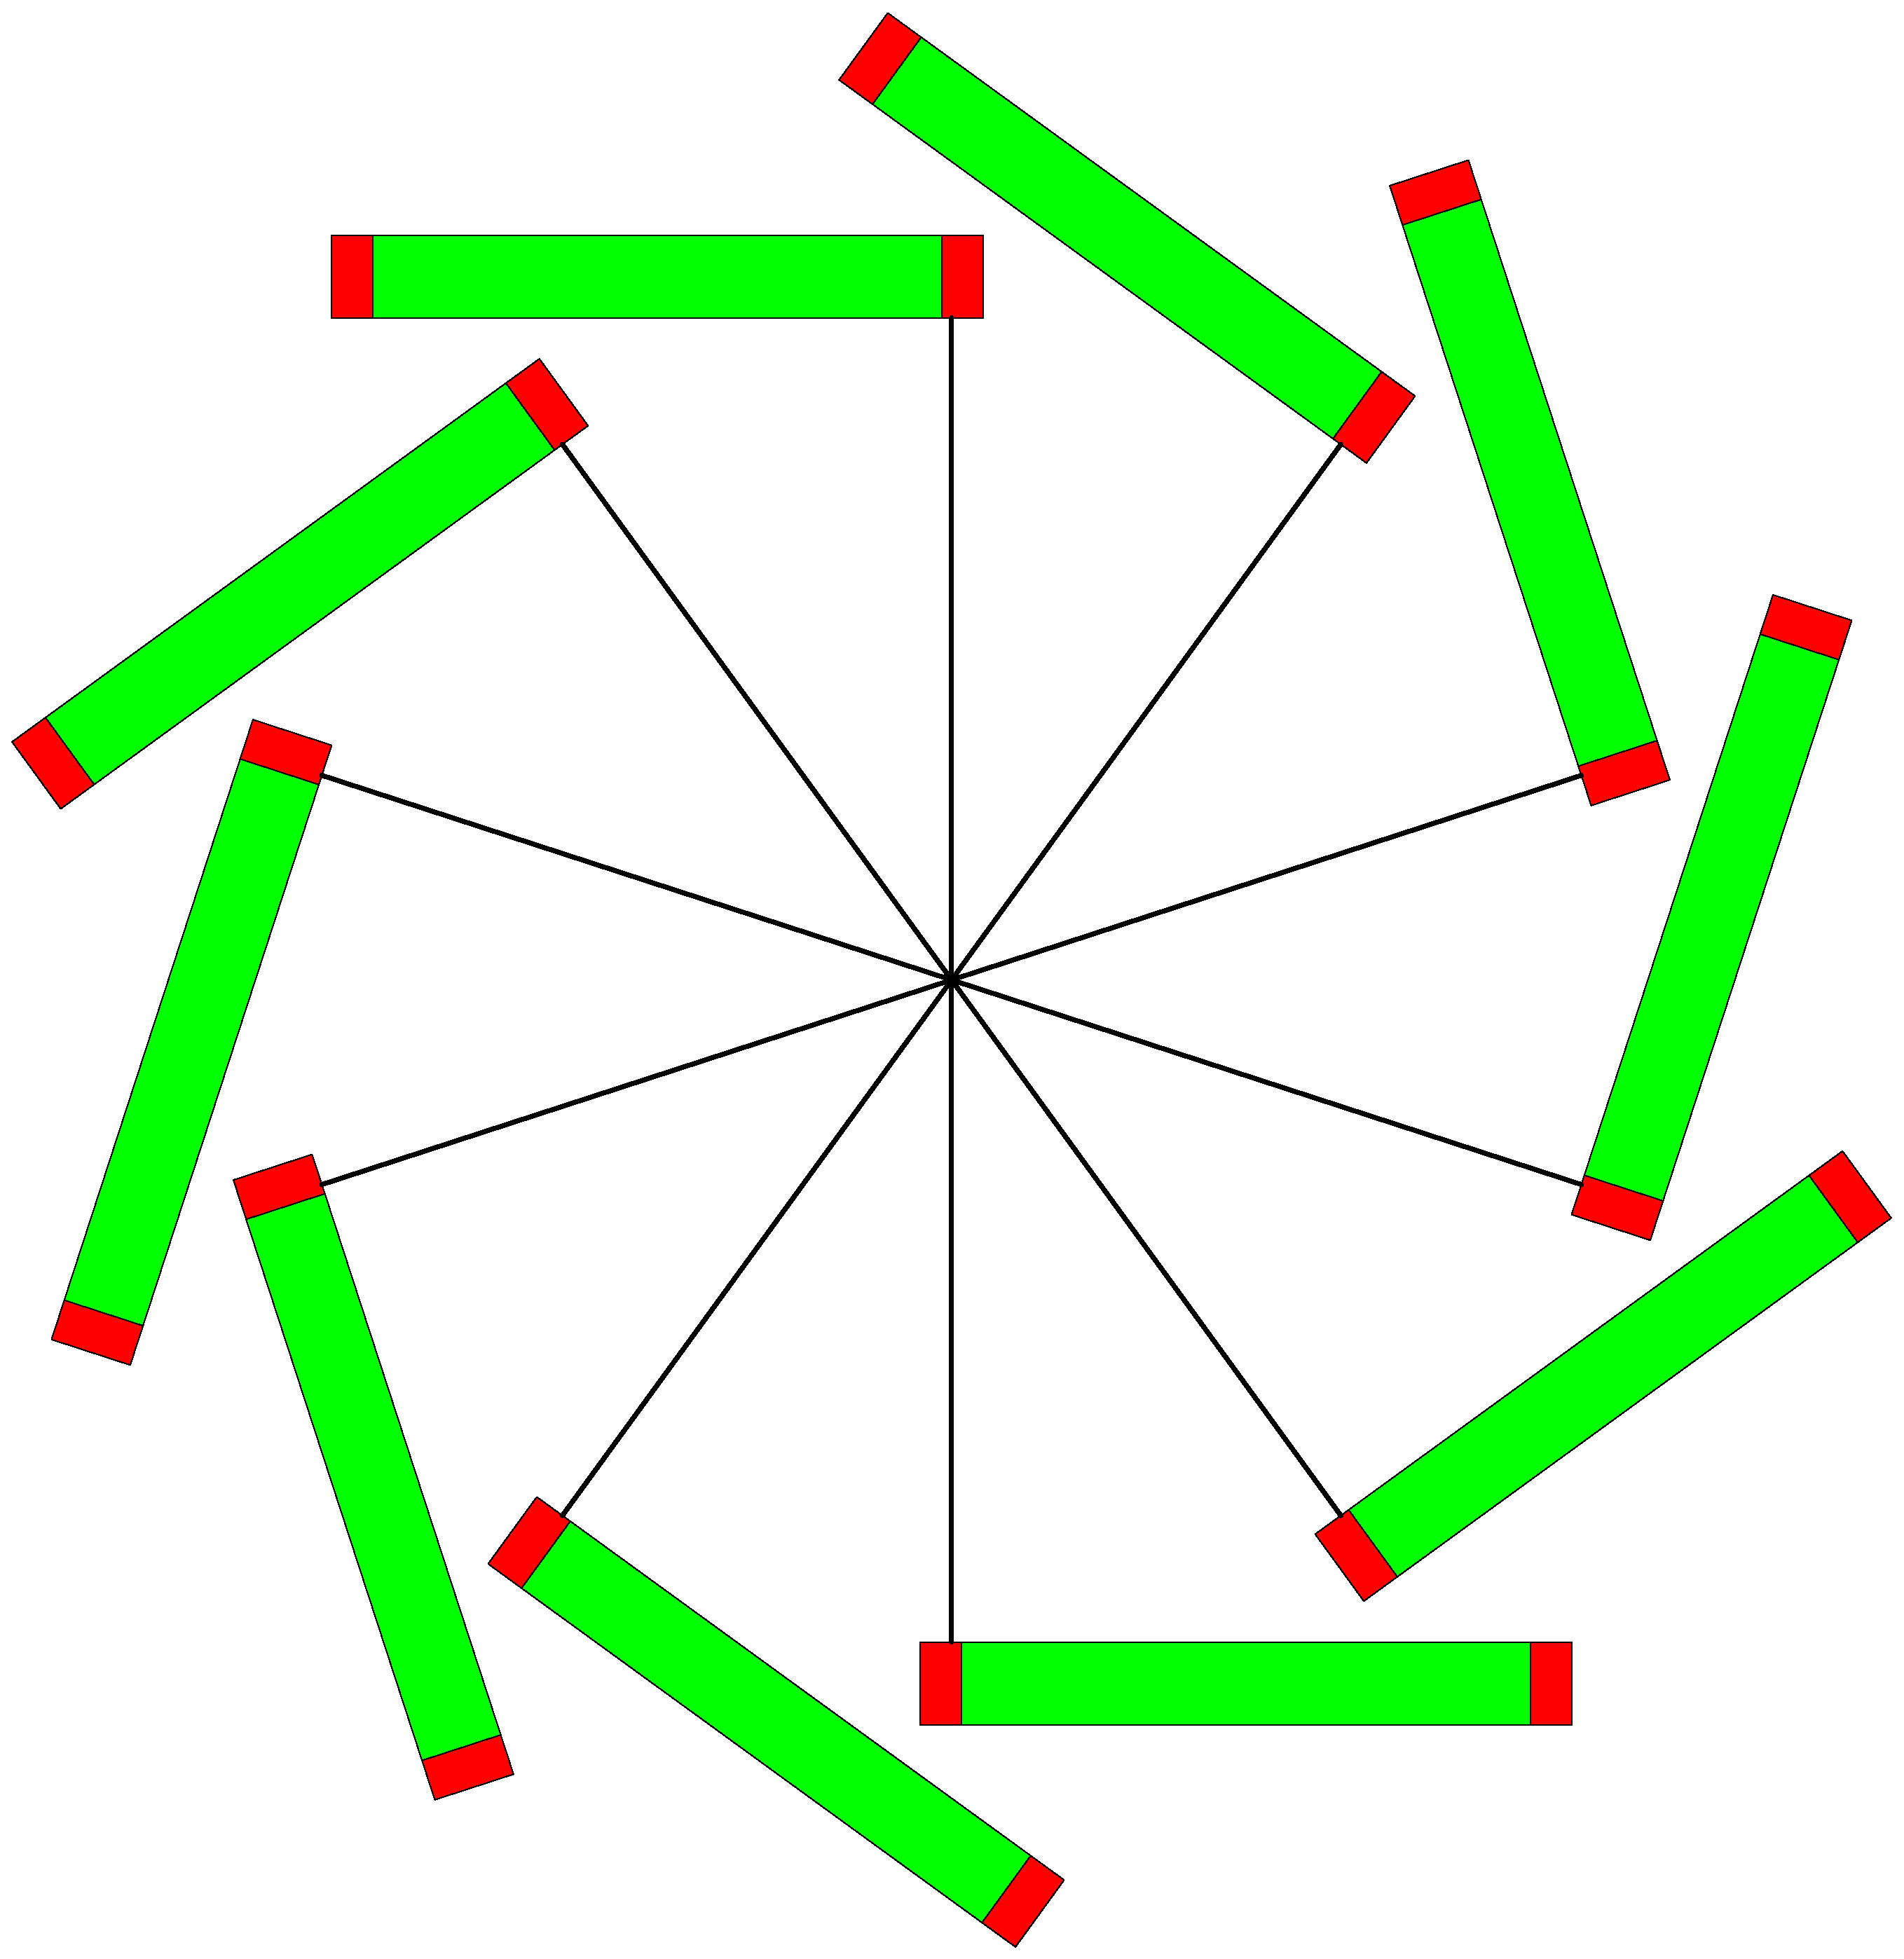
\includegraphics[width=0.37\textwidth]{./figures/CalculsRecouvrment/Scripts_Asymptote/DL1_option1_final_2mm.eps}
        }
        \subfigure[Option 2 : Configuration pour la premi\`ere double couche avec 10 \'echelles de 1 $mm$ d'\'epaisseur.Les zones pixelis\'ees sont repr\'esent\'ees en vert et les zones de Lecture/traitement de l'information sont repr\'esent\'ees en rouge.]{
            \label{fig:DL1_1mm}
            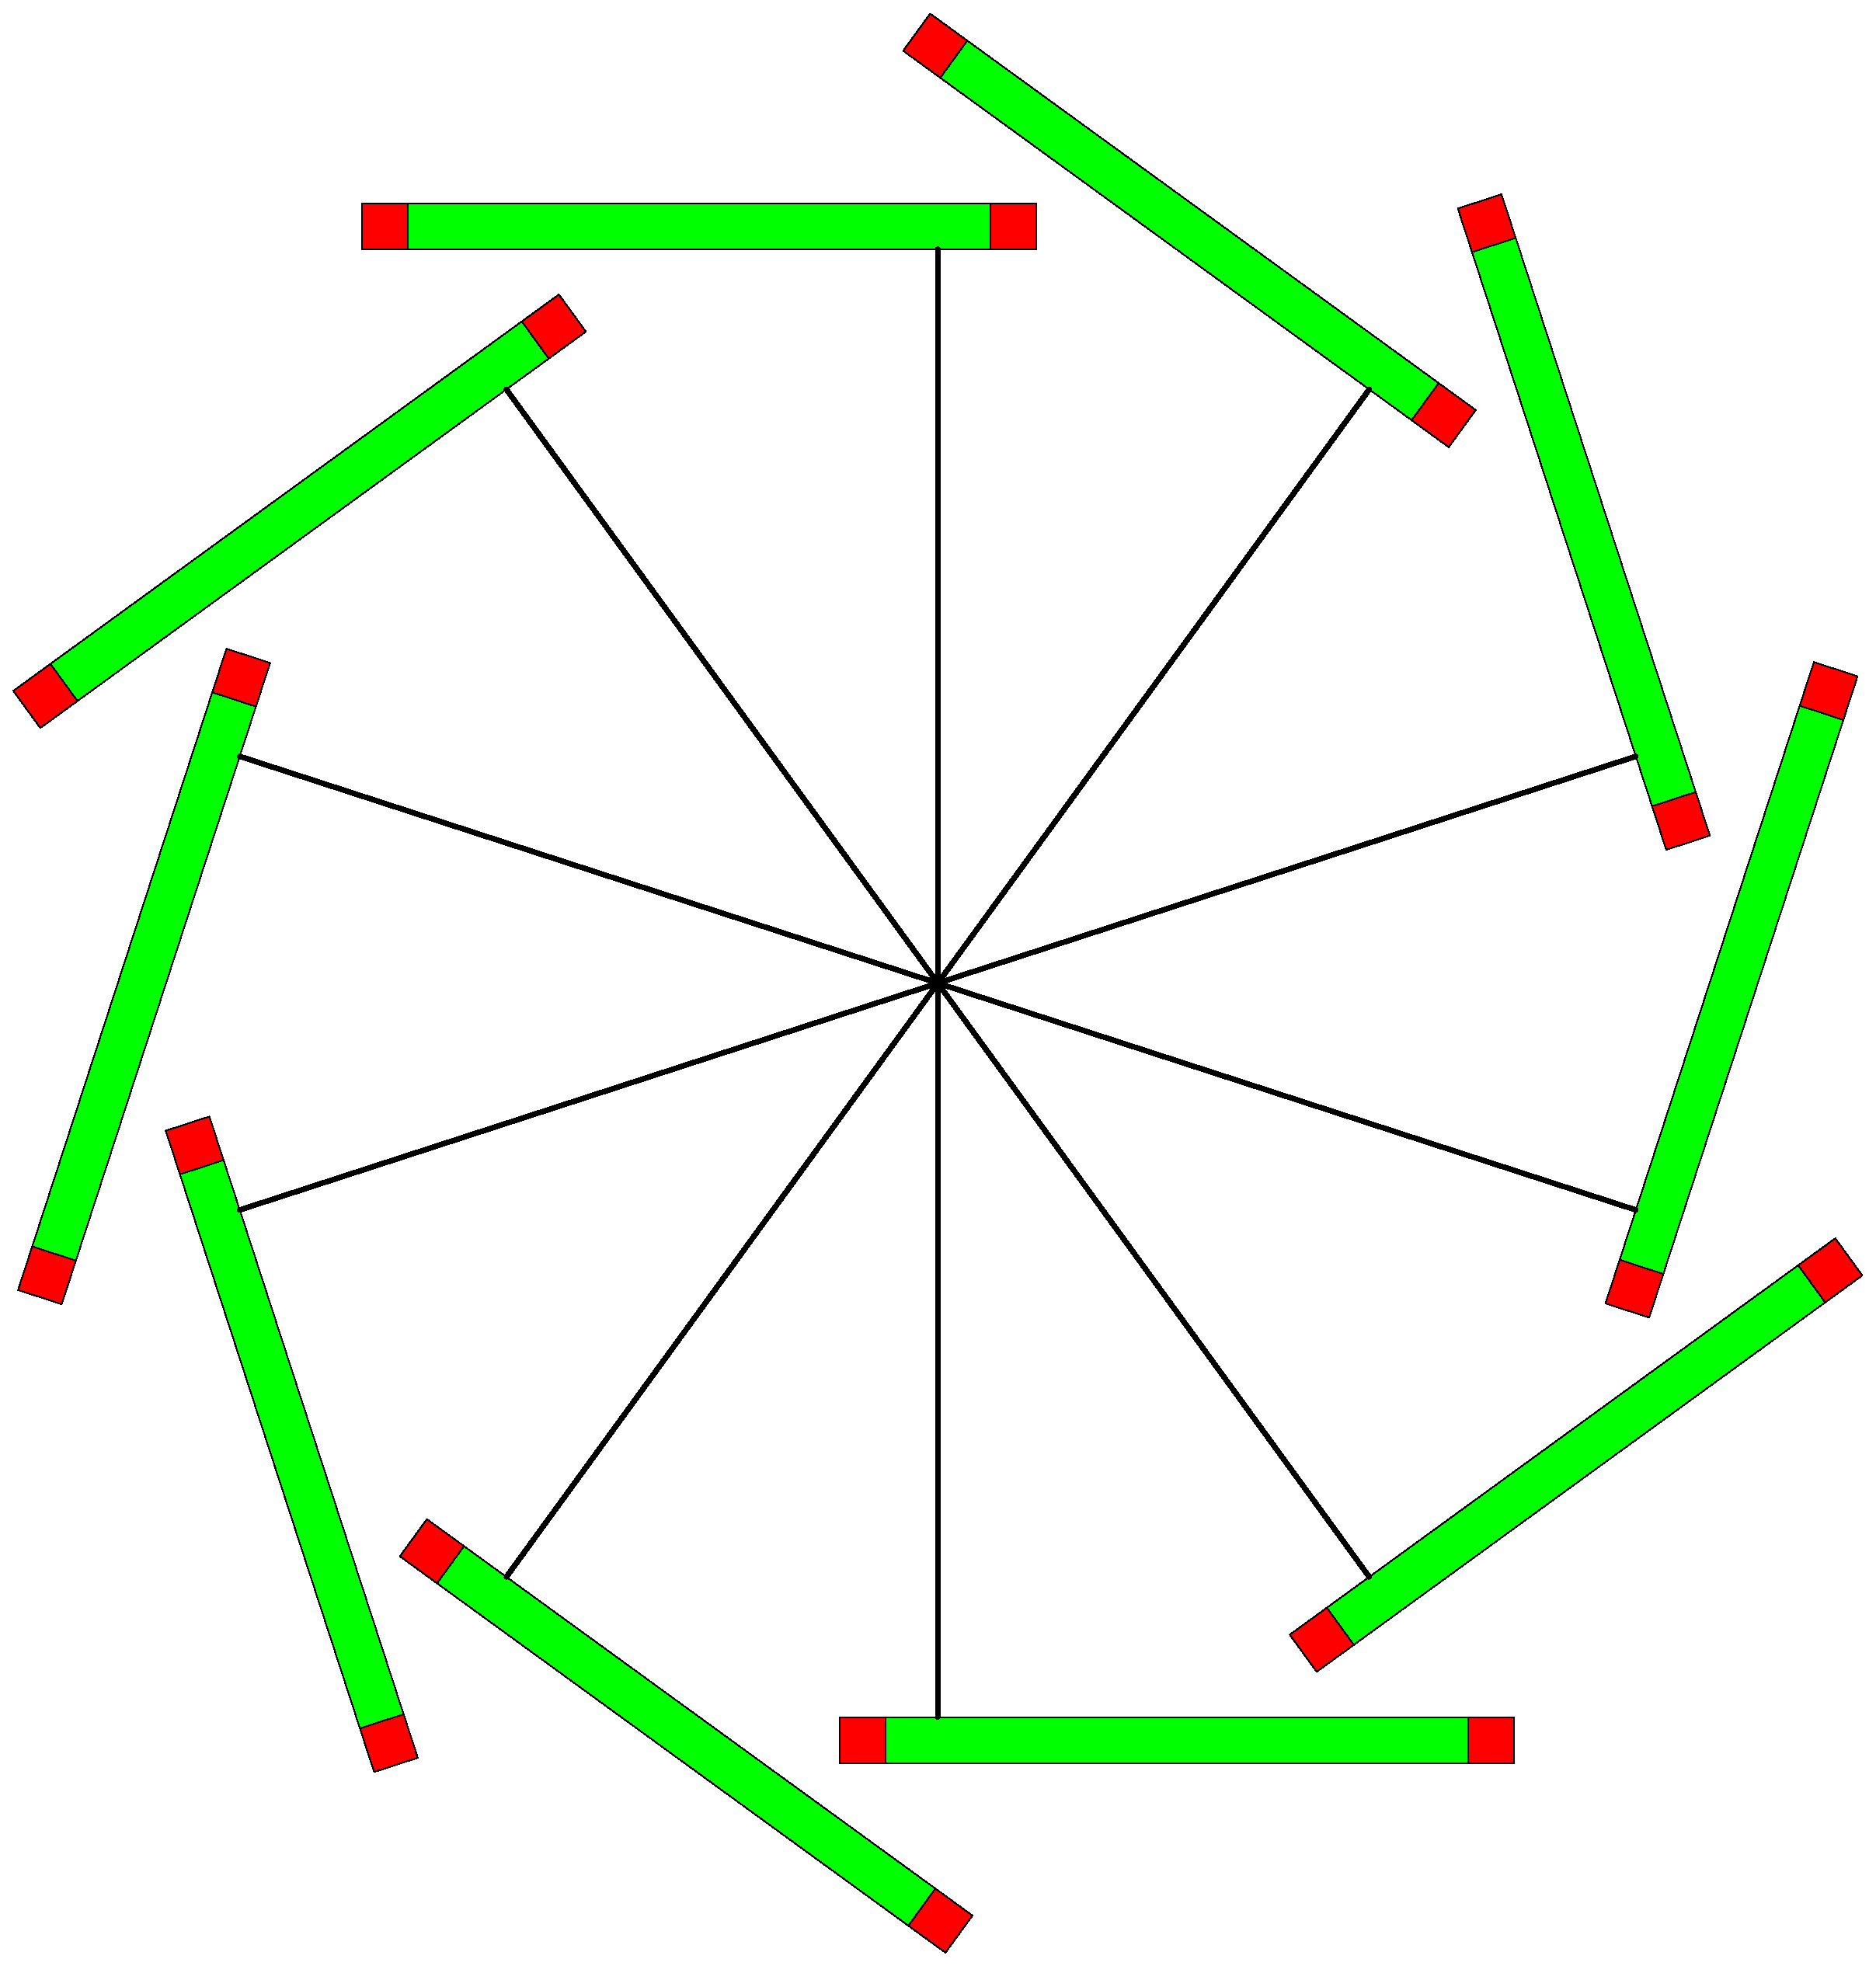
\includegraphics[width=0.37\textwidth]{./figures/CalculsRecouvrment/Scripts_Asymptote/DL1_option1_final.eps}
        }
     \end{center}
     \caption{Repr\'esentation de la premi\`ere double couche du d\'etecteur de vertex.}
     \label{fig:DL1geometryOptions}
   \end{figure}

   \begin{figure}[htb!]
     \begin{center}
        \subfigure[Configuration pour la seconde double couche avec 13 \'echelles de 2 $mm$ d'\'epaisseur. Les zones pixelis\'ees sont repr\'esent\'ees en vert et les zones de Lecture/traitement de l'information sont repr\'esent\'ees en rouge.]{
            \label{fig:DL2_2mm}
            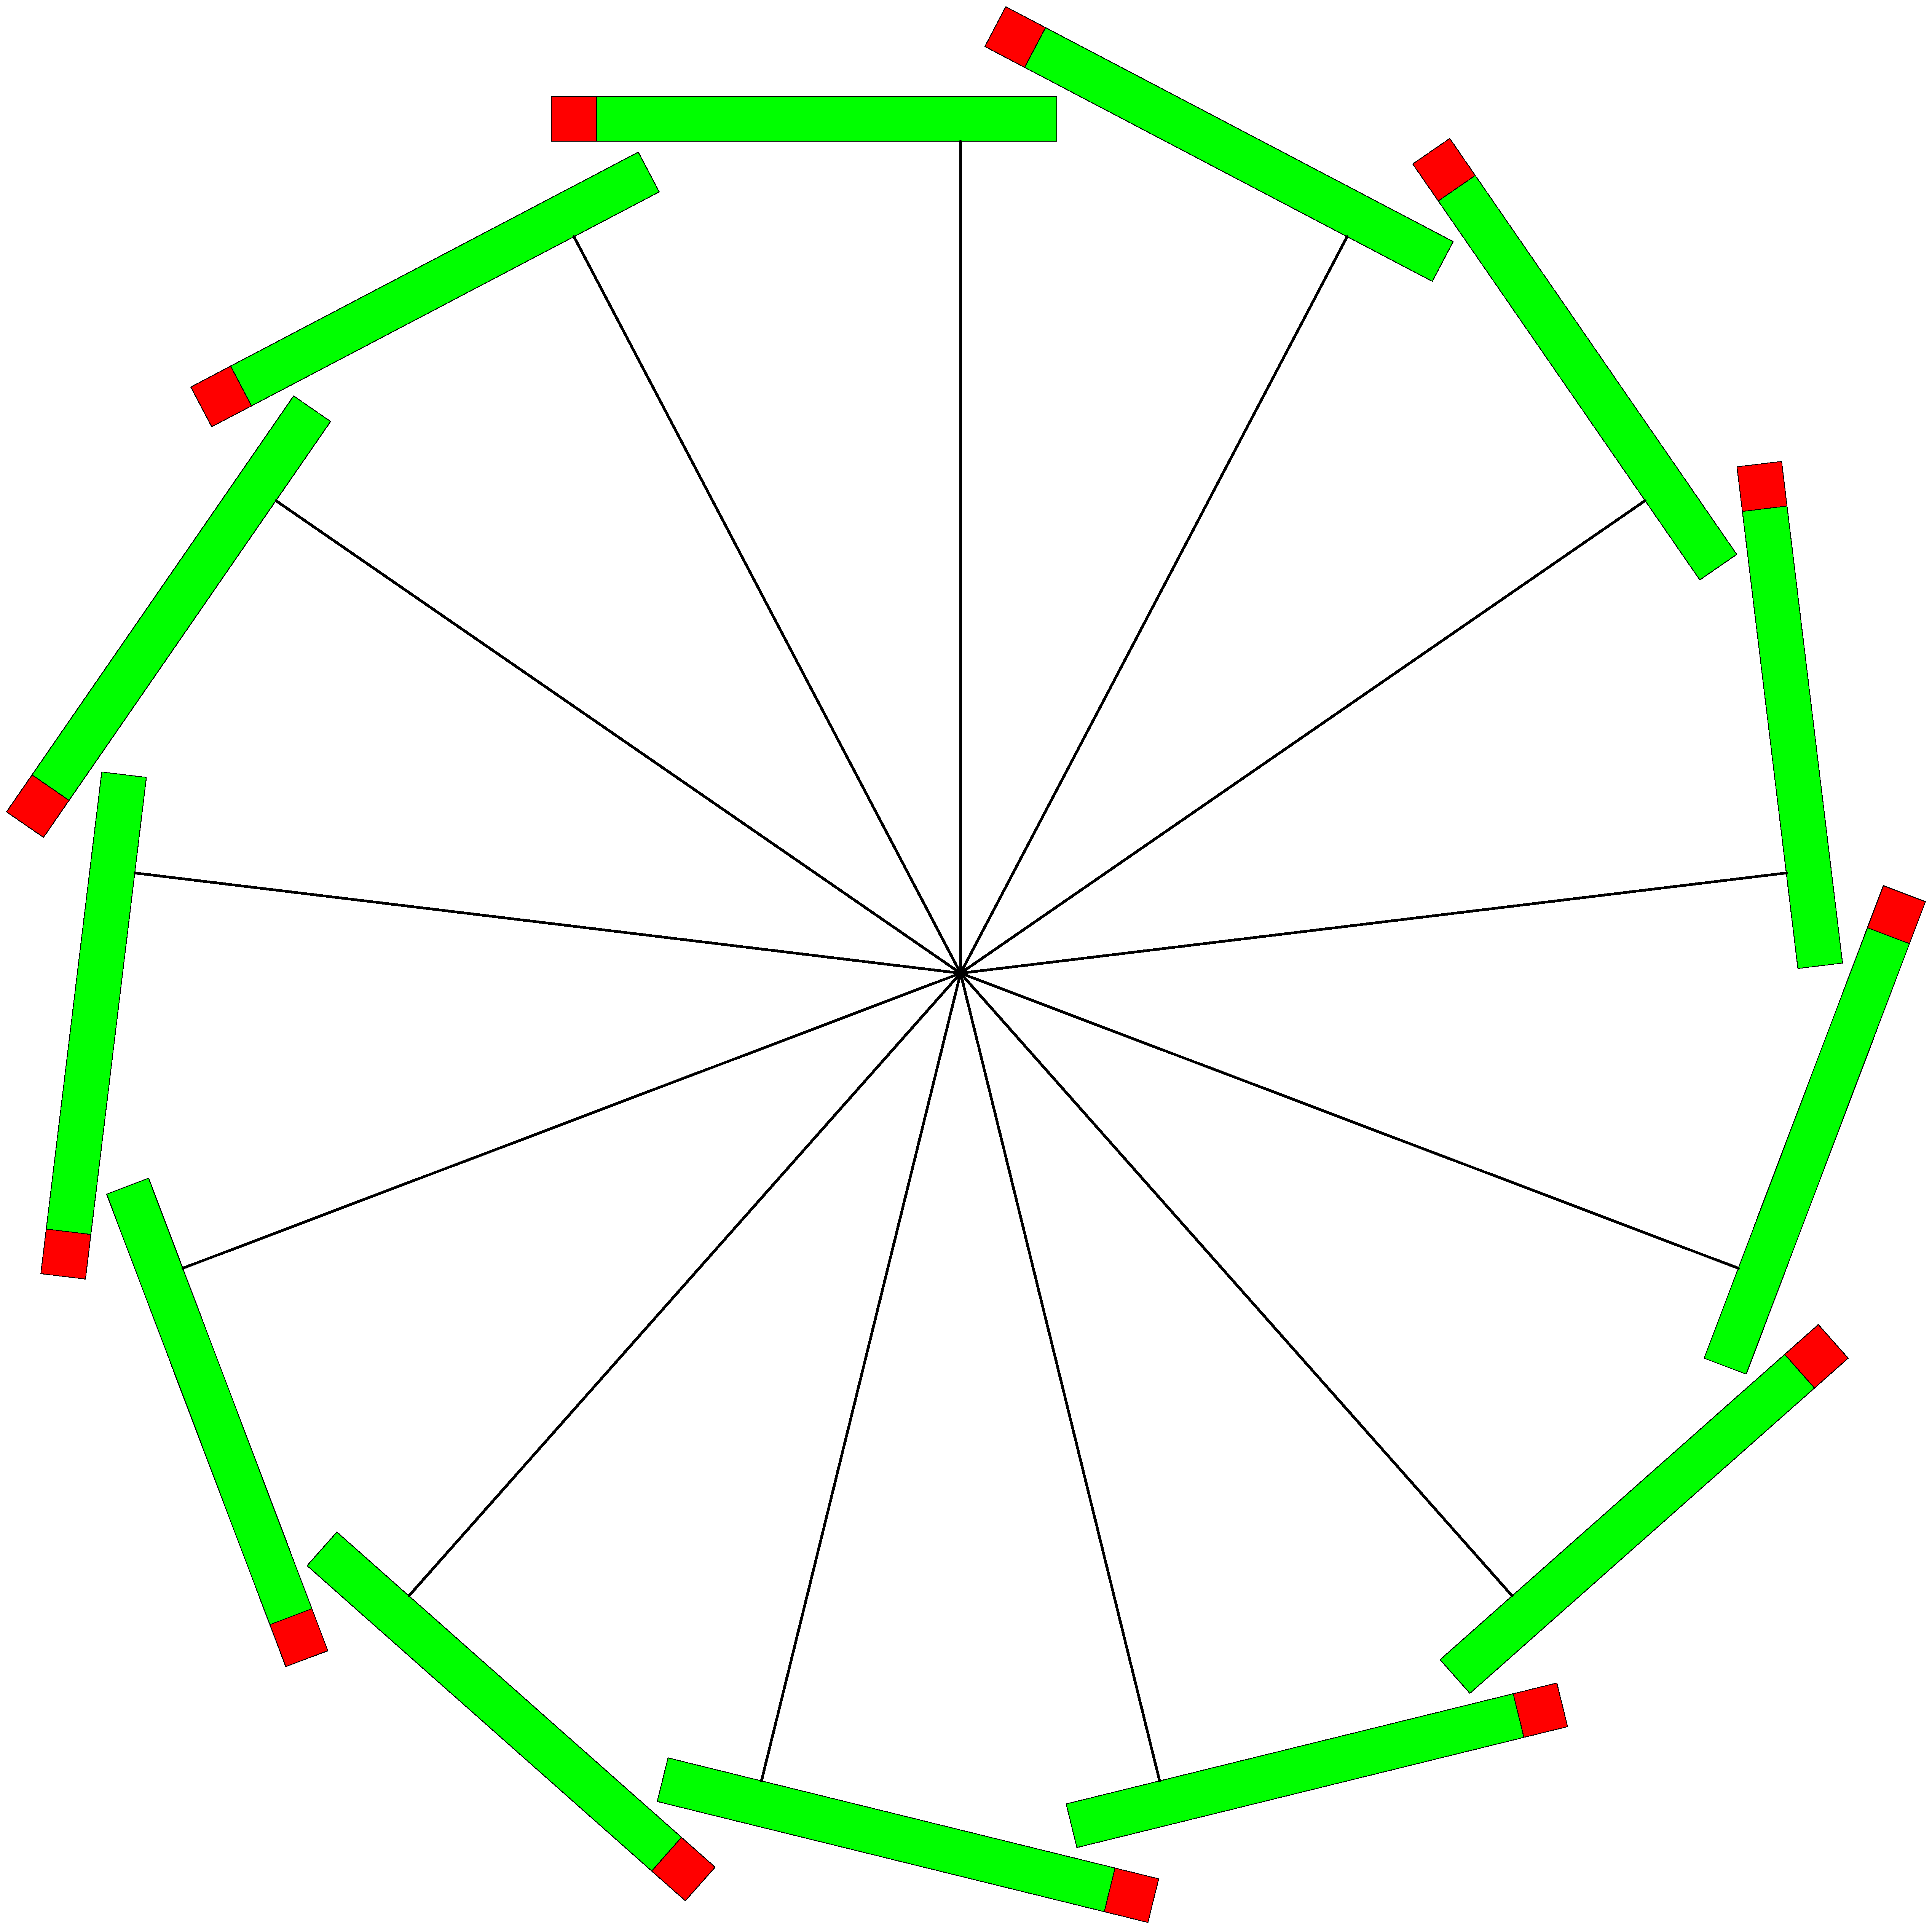
\includegraphics[width=0.37\textwidth]{./figures/CalculsRecouvrment/Scripts_Asymptote/DL2_option1_final.eps}
        }
        \subfigure[Configuration pour la troisi\`eme double couche avec 19 \'echelles de 2 $mm$ d'\'epaisseur.Les zones pixelis\'ees sont repr\'esent\'ees en vert et les zones de Lecture/traitement de l'information sont repr\'esent\'ees en rouge.]{
            \label{fig:DL3_2mm}
            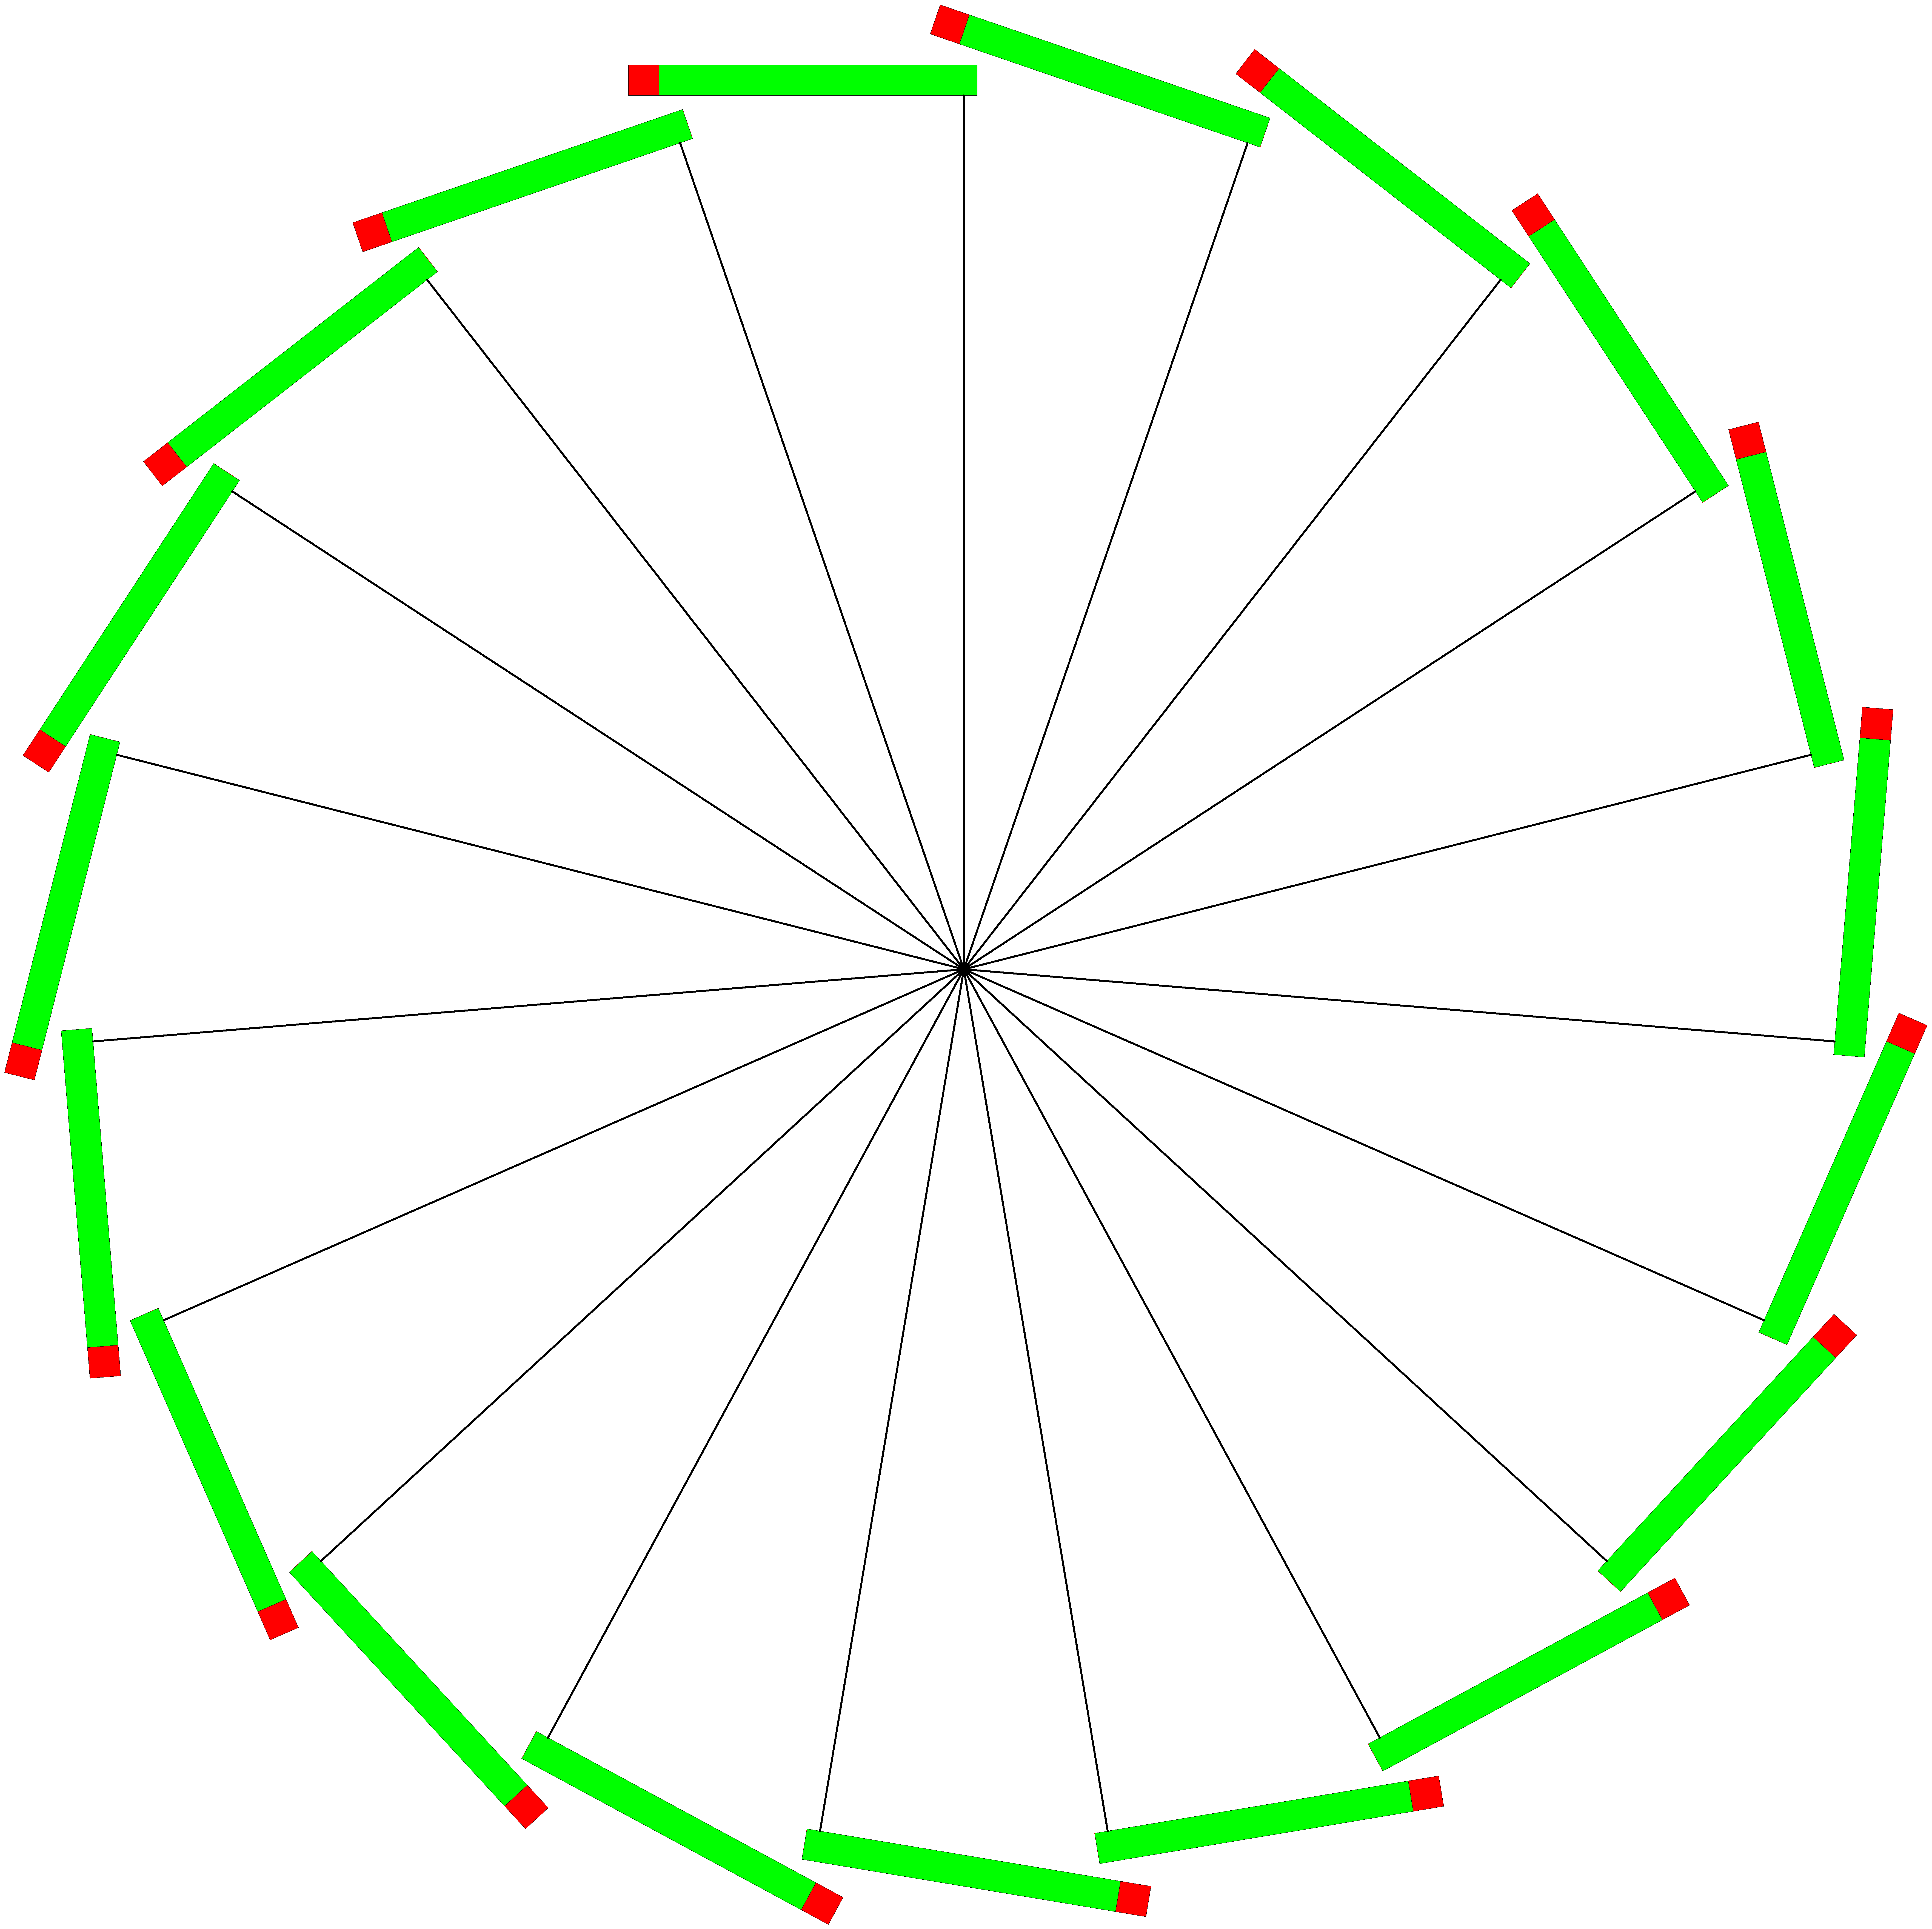
\includegraphics[width=0.37\textwidth]{./figures/CalculsRecouvrment/Scripts_Asymptote/DL3_option1_final.eps}
        }
     \end{center}
     \caption{Repr\'esentation de la seconde et de la troisi\`eme double couche du d\'etecteur de vertex.}
     \label{fig:DL23geometryOptions}
   \end{figure}
   
   \medskip
   
   La figure \ref{fig:DL1geometryOptions} repr\'esente la premi\`ere double couche du d\'etecteur de vertex d\'ecrite \`a l'aide des calculs pr\'ec\'edant. On peut voir sur cette figure, deux options possibles, l'une utilisant des \'echelles d'une \'epaisseur de 2 $mm$ et l'autre utilisant des \'echelles de 1 $mm$ d'\'epaisseur. Cette seconde option a \'et\'e jug\'ee utile puisque la configuration utilisant des \'echelles de 2 $mm$ d'\'epaisseur poss\`ede d'importantes zones o\`u les traces peuvent croiser deux \'echelles successives de la premi\`ere double couche. Cela augmente le budget de mati\`ere de la double couche. Ainsi, afin de r\'eduire le budget de mati\`ere et ces zones de recouvrement, on pr\'ef\'erera utiliser des \'echelles de seulement 1 $mm$ d'\'epaisseur.
   
   \medskip
   
   La seconde et la troisi\`eme double couche sont repr\'esent\'ees en figure \ref{fig:DL23geometryOptions}. Afin de r\'eduire le co\^ut de fabrication, ces deux double couche pourront \^etre \'equip\'ees des m\^emes capteurs. Il faudra donc optimiser la hauteur des \'echelles afin d'utiliser des capteurs de m\^eme taille. Lorsque l'on effectue les calculs ci-dessus, on constate que pour des capteurs d'environ 2 $cm$ de hauteur et un recouvrement de 500 $\mu m$, il faut utiliser 13 \'echelles pour la seconde double couche et 19 \'echelles pour la troisi\`eme double couche. Le tableau \ref{tab:geomResults} r\'esume les valeurs obtenues pour chaque double couche. Lorsque l'on se concentre sur les valeurs des rayons de ces deux double couche d\'etermin\'ees pour le \textit{DBD} \`a savoir $R_2 = 37 mm$ et $R_3 = 58 mm$, on trouve des tailles de capteurs de respectivement $L_2 = 22.612 mm$ et $L_3 = 23.064 mm$. Cela repr\'esente une diff\'erence de 452 $\mu m$. Afin de conserver un recouvrement et une taille de capteur identiques, on peut choisir de l\'eg\`erement r\'eduire ou agrandir le rayon des doubles couches 2 et 3. On peut alors calculer le rayon de la double couche 3 en fonction de la double couche 2 \`a recouvrement et taille de capteur identiques. Afin d'effectuer ce calcul on calcule les tailles totales $L_2$ et $L_3$ des capteurs pour les doubles couches 2 et 3 :
  
  \begin{equation}
   L = L_{int} + \Delta L + X + bordGauche
  \end{equation}

  Ce qui donne apr\`es calcul :
  
  \begin{align}
   L = \left[ \cfrac{\sin{\theta}}{\cos{\theta}}  + \left( \cfrac{\cos{\theta} - 1}{\cos{\theta}} \right) \left( \sin{\theta} + \cfrac{\cos{\theta} - 1}{\sin{\theta}} \cos{\theta} \right) \right] Rayon \\ \nonumber
   + \cfrac{bordDroit + Recouvrement + Epaisseur \sin{\theta}}{\cos{\theta}} \\ \nonumber
   - \left( 1 - \cfrac{1}{\cos{\theta}} \right) \left( offSetX + \cfrac{Epaisseur + offSetY}{\sin{\theta}} \cos{\theta} \right) + bordGauche
  \end{align}  

  On peut alors r\'e\'ecrire ce terme de la fa\c{c}on suivante :
  
  \begin{equation}
   L_i = A_i \, Rayon_i + B_i
   \label{eq:long_sensor}
  \end{equation}

  Avec l'indice $i$ correspondant au num\'ero de la double couche et les constantes $A_i$ et $B_i$ valant :
  
  \begin{equation}
   A_i = \cfrac{\sin{\theta_i}}{\cos{\theta_i}}  + \left( \cfrac{\cos{\theta_i} - 1}{\cos{\theta_i}} \right) \left( \sin{\theta_i} + \cfrac{\cos{\theta_i} - 1}{\sin{\theta_i}} \cos{\theta_i} \right)
  \end{equation}

  \begin{align}
   B_i = + \cfrac{bordDroit_i + Recouvrement_i + Epaisseur_i \sin{\theta_i}}{\cos{\theta_i}} \\ \nonumber
   - \left( 1 - \cfrac{1}{\cos{\theta_i}} \right) \left( offSetX_i + \cfrac{Epaisseur_i + offSetY_i}{\sin{\theta_i}} \cos{\theta_i} \right) + bordGauche_i
  \end{align}
  
  On \'egalise alors $L_2 = L_3$ :

  \begin{equation}
   A_2 Rayon_2 + B_2 = A_3 Rayon_3 + B_3
  \end{equation}

  On obtient alors la valeur du rayon de la troisi\`eme double couche en fonction de celui de la seconde double couche, pour un recouvrement et une taille de capteur identique :
  
  \begin{equation}
   Rayon_3 = \cfrac{A_2}{A_3} \, Rayon_2 + \cfrac{B_2 - B_3}{A_3}
   \label{eq:R3_R2}
  \end{equation}

%   \begin{figure}[!htb]
%     \begin{center}
%       \includegraphics[scale=0.7]{./figures/CalculsRecouvrment/Scripts_Asymptote/R3_function_of_R2.pdf}
%       \caption{Relation entre les rayons des double couche 2 et 3 pour obtenir un recouvrement et une taille de capteur identiques.}
%       \label{fig:R3_vs_R2}
%     \end{center}
%   \end{figure}
%   
%   \begin{figure}[!htb]
%     \begin{center}
%       \includegraphics[scale=0.7]{./figures/CalculsRecouvrment/Scripts_Asymptote/L_function_of_R2.pdf}
%       \caption{Taille des capteurs des double couche 2 et 3 en fonction du rayon de la seconde double couche. Cette taille est obtenue pour un recouvrement et taille de capteur identiques pour les double couche 2 et 3.}
%       \label{fig:L_vs_R2}
%     \end{center}
%   \end{figure}
%   
%   La figure \ref{fig:R3_vs_R2} illustre l'\'equation \ref{eq:R3_R2}. Les valeurs utilis\'ees pour cette repr\'esentation sont list\'ees dans le tableau \ref{tab:geomResults}. On peut de plus calculer gr\^ace \`a l'\'equation \ref{eq:long_sensor} la longueur des capteurs pour des rayons $Rayon_2$ et $Rayon_3$ donn\'es. La figure \ref{fig:L_vs_R2} donne la taille des capteurs des doubles couches 2 et 3 en fonction du rayon de la seconde double couche. Ainsi gr\^ace \`a ces deux graphes, on peut s\'electionner une taille de capteur puis trouver les rayons correspondant pour les double couche 2 et 3.
  
  La relation \ref{eq:long_sensor} donne la taille total des capteurs des doubles couches 2 et 3 en fonction du rayon de leur double couche. La relation \ref{eq:R3_R2} lie les rayons des doubles couches 2 et 3 lorsque le recouvrement et la taille des capteurs sont identiques. On peut donc facilement choisir une m\^eme taille totale pour les capteurs des doubles couches 2 et 3 et d\'eterminer les rayons des doubles couches 2 et 3 correspondants.
  
  \medskip
  
  Le tableau \ref{tab:geomResults} r\'esume les valeurs obtenues pour chaque double couche en fonction de l'option choisie. Les param\`etres utilis\'es pour le \textit{DBD} sont \'etiquetés \textit{option1}. Pour les doubles couches 2 et 3, l'\textit{option2} renseigne sur les rayons calcul\'es pr\'ec\'edemment pour les doubles couches 2 et 3 pour obtenir une taille de capteur et un recouvrement constant ; et correspondant aux valeurs des rayons de 37 $mm$ et 58 $mm$ du \textit{DBD}.
  
 \medskip
 
  Enfin, la figure \ref{fig:recouvrement_DL1_DL2_DL3} est une illustration des trois double couche r\'eunies sur un m\^eme graphique. On notera qu'un offset peut \^etre utilis\'e afin de tourner les doubles couches les unes par rapport aux autres. Cela permet de r\'epartir le budget de mati\`ere du d\'etecteur de vertex. En effet, le budget de mati\`ere est plus important aux niveau de chaque zone de recouvrement et il est pr\'ef\'erable de ne pas aligner les zones de recouvrement de chacune des couches afin d'homog\'en\'eiser le budget de mati\`ere. Pour la figure \ref{fig:recouvrement_DL1_DL2_DL3} aucun offset n'est utilis\'e.
  
\begin{sidewaystable}
\begin{tabular}{|l|l|l|l|l|l|l|} \hline
\textbf{Double Couche}            & \textbf{DL1 option1} & \textbf{DL1 option2} & \textbf{DL2 option1} & \textbf{DL2 option2} & \textbf{DL3 option2} & \textbf{DL3 option1} \\ \hline
\textbf{Rayon $[mm]$}           & 16                   & 16                   & 37 fix\'e               & 37.917               & 56.6456              & 58 fix\'e               \\ \hline
\textbf{Epaisseur $[mm]$}       & 1                    & 2                    & 2                    & 2                    & 2                    & 2                    \\ \hline
\textbf{\'Echelles}                  & 10                   &                      & 13                   & 13                   & 19                   & 19                   \\ \hline
\textbf{Angle $[rad]$}          & $2 \pi / 10$           & 2 $\pi / 10$           & 2 $\pi /13$            & $2 \pi /13$            & $2 \pi/ 19$            & $2 \pi/ 19$            \\
\textbf{bordDroit $[\mu m]$}    & 1                    & 1                    & 0                    & 0                    & 0                    & 0                    \\ \hline
\textbf{bordGauche $[\mu m]$}   & 1                    & 1                    & 2                    & 2                    & 2                    & 2                    \\ \hline
\textbf{offSetX}                  & $1/\sqrt{2}$          & $1/\sqrt{2}$          & $1/\sqrt{2}$          & $1/\sqrt{2}$          & $1/\sqrt{2}$          & $1/\sqrt{2}$          \\ \hline
\textbf{offSetY}                  & $1/\sqrt{2}$          & $1/\sqrt{2}$          & $1/\sqrt{2}$          & $1/\sqrt{2}$          & $1/\sqrt{2}$          & $1/\sqrt{2}$          \\ \hline
\textbf{X $[mm]$}               & 2.142                & 0.766                & 3.255                & 3.481                & 0.860                & 1.086                \\ \hline
\textbf{Lint $[mm]$}            & 8.103                & 9.804                & 14.945               & 15.171               & 17.790               & 18.016               \\ \hline
\textbf{DeltaL $[mm]$}          & 3.455                & 4.181                & 2.413                & 2.413                & 1.963                & 1.963                \\ \hline
\textbf{Recouvrement $[\mu m]$} & 500                  & 500                  & 500                  & 500                  & 500                  & 500                  \\ \hline
\textbf{Lpixels $[mm]$}         & 12.700               & 13.751               & 20.612               & 21.064               & 20.612               & 21.064               \\ \hline
\textbf{L Totale $[mm]$}        & 14.700               & 15.751               & 22.612               & 23.064               & 22.612               & 23.064 \\ \hline             
\end{tabular}
\caption{Valeurs obtenues pour les param\`etres des double couche apr\`es calculs.}
\label{tab:geomResults}
\end{sidewaystable}

  
  \begin{figure}[!htb]
    \begin{center}
      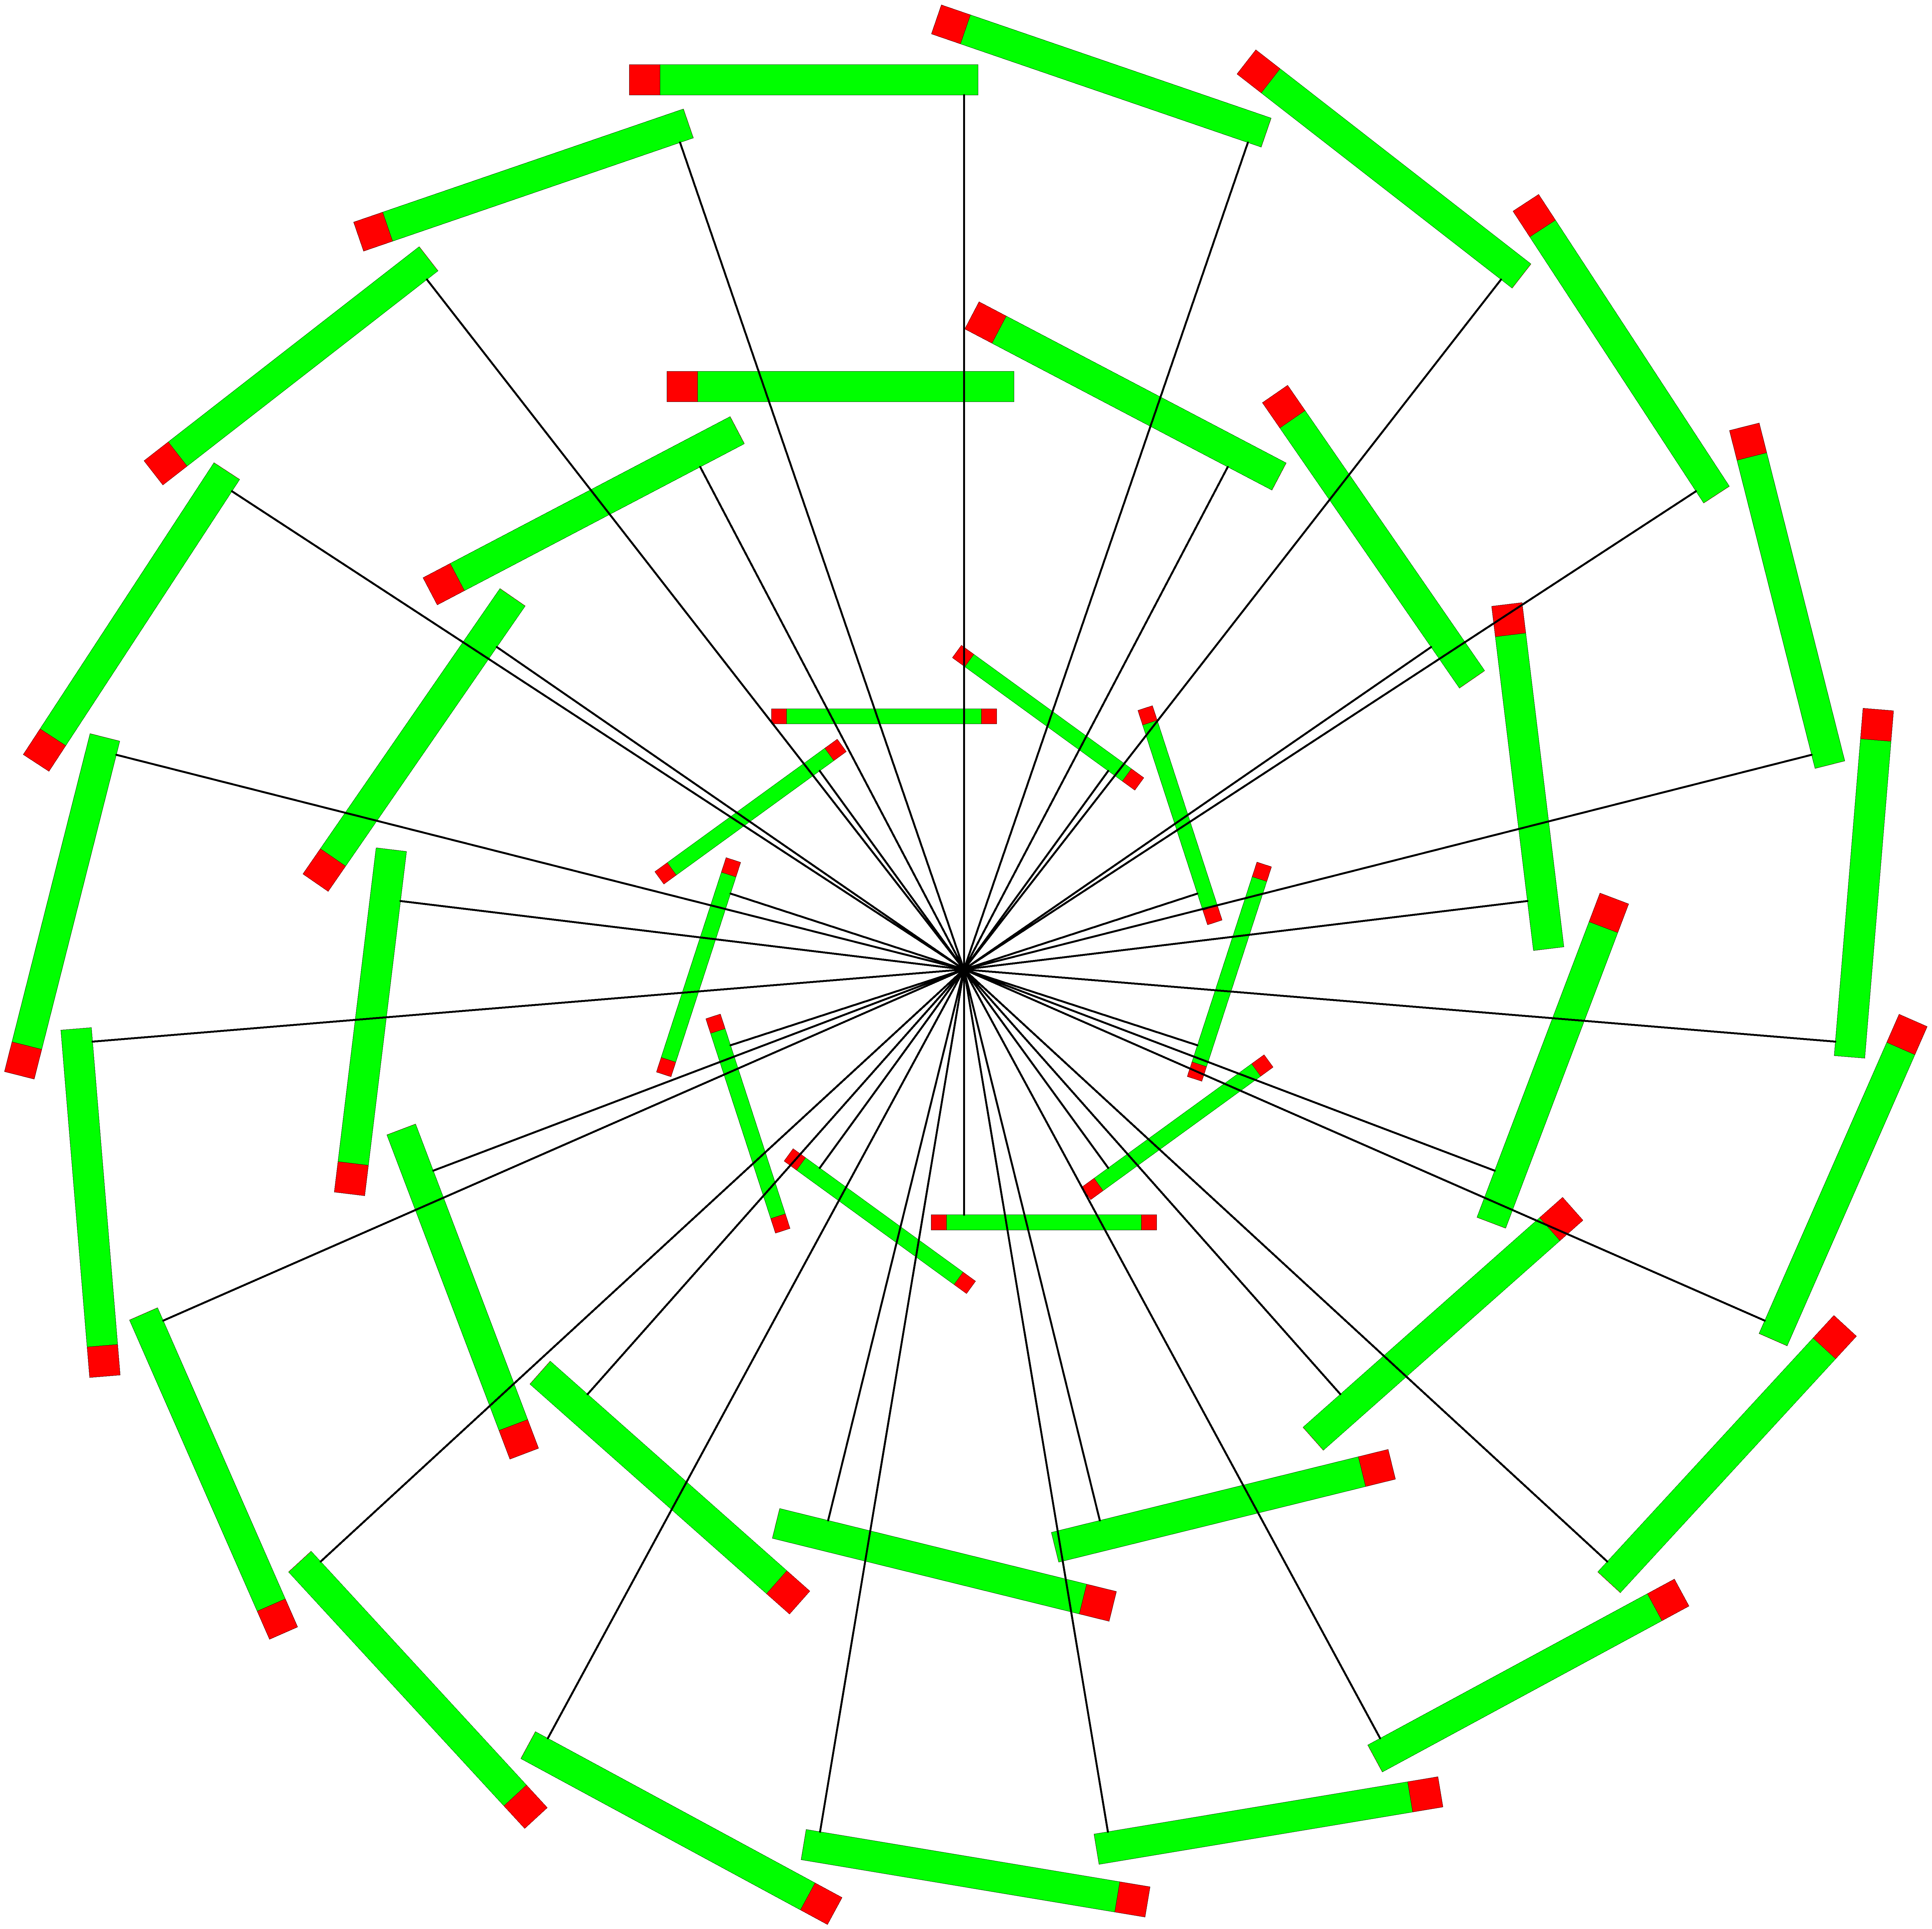
\includegraphics[scale=0.1]{./figures/CalculsRecouvrment/DL1_DL2_DL3_option1.eps}
      \caption{Sch\'ema des trois double couche du d\'etecteur de vertex r\'eunies. Aucun offset n'est utilis\'e.}
      \label{fig:recouvrement_DL1_DL2_DL3}
    \end{center}
  \end{figure}

\section{Alignement bas\'e sur les mini-vecteurs}
  
  Les \'echelles doubles faces de capteurs CMOS, permettent la cr\'eation de mini-vecteurs. Ces mini-vecteurs permettent \`a priori un alignement des doubles couches du d\'etecteur de vertex grace aux zones de recouvrement entre \'echelles successives. L'id\'ee est d'effectuer un alignement de la double couche en se servant uniquement des mini-vecteurs sur les zones recouvrement des échelles de la double couche consid\'er\'ee.
  
  \medskip
  
  Afin de voir si cette id\'ee ambitieuse est r\'ealisable ou non, nous allons dans un premier temps voir dans quelle mesure on peut aligner une \'echelle double face fixe par rapport \`a une autre mobile, \`a l'aide des mini-vecteurs reconstruits dans la zone de recouvrement des deux échelles. Cela revient \`a aligner deux \'echelles cons\'ecutives d'une double couche de d\'etecteur de vertex. Nous verrons dans un premier temps comment la reconstruction des mini-vecteurs est r\'ealis\'ee, nous d\'ecrirons ensuite la g\'eom\'etrie utilis\'ee pour r\'ealiser cette \'etude ; puis, nous pr\'esenterons la m\'ethode d'alignement avec mini-vecteurs. Notre m\'ethode d'alignement utilise des traces sctrictement rectilignes, c'est \`a dire qu'aucun champ magn\'etique n'est utilis\'e. Nous allons alors r\'ealiser des alignements \`a haute impulsion ($p = 120GeV/c$) afin de savoir si notre m\'ethode d'alignement est viable ou non.

  \subsection{R\'ealisation des mini-vecteurs}
  \label{realisation_MV}
  
  Les mini-vecteurs sur chacune des \'echelles utilis\'ees sont r\'ealis\'es de la façon suivante. Sur chaque \'echelle, on identifie les impacts sur la face de l'\'echelle croisant le faisceau en premier. Puis, \`a chacun de ces impacts, l'impact le plus proche sur la face oppos\'ee est s\'electionné. Il s'agit l\`a de la façon la plus simple pour r\'ealiser des mini-vecteurs.
  
  \medskip  
  
%   Cependant, l'application des coupures sur la distance maximale et les pentes du mini-vecteur permettent d'exclure les mauvais mini-vecteurs.
  Dans la suite de ce chapitre nous utiliserons une seule trace par \'ev\'enement afin de caract\'eriser la m\'ethode d'alignement avec mini-vecteurs. Il s'agit ici de montrer les pr\'ecisions et possibilit\'es de la m\'ethode dans un cadre id\'eal. Un travail avec plusieurs traces par \'ev\'enement a \'et\'e d\'ebut\'e mais celui-ci n'est pas encore mature \`a l'heure de la r\'edaction de ce chapitre.
 
  \subsection{Description de l'algorithme d'alignement}
  \label{sect:algo_align_MV}
 
  Nous allons \`a pr\'esent d\'ecrire la m\'ethode d'alignement de deux \'echelles doubles faces successives, gr\^ace aux mini-vecteurs reconstruits \`a l'int\'erieur de leur zone de recouvrement.
 
   \paragraph{Principe de fonctionnement}
   
   Nous voulons aligner une \'echelle double face mobile (\'echelle 1) par rapport \`a une \'echelle double face fixe (\'echelle 0). Pour cela nous consid\'ererons des \'echelles "parfaites" c'est \`a dire sans d\'eformation. Aucun champ magn\'etique n'est pr\'esent. Le faisceau utilis\'e est compos\'e de pions n\'egatifs dot\'es d'une impulsion de 120 $GeV/c$. Du fait de cette haute impulsion, les traces reconstruites sont consid\'er\'ees rectilignes. Notre m\'ethode d'alignement aligne le centre et les inclinaisons de l'\'echelle mobile par rapport \`a l'\'echelle fixe, prise comme r\'ef\'erence. Nous allons nous baser sur le cas d'une \'echelle mobile et d\'esalign\'ee, comme sch\'ematis\'ee en figure \ref{fig:schema_MV}. La m\'ethode d'alignement peut se d\'ecomposer en plusieurs \'etapes. Nous allons les d\'ecrire.
   
   \medskip
   
  \begin{figure}[!htb]
    \begin{center}
      \includegraphics[scale=1.25]{./figures/mini_vecteurs-schema.png}
      \caption{Sch\'ema de principe de la m\'ethode d'alignement avec mini-vecteurs. L'\'echelle fixe (\'echelle 0) est illustr\'ee en bleu et l'\'echelle \`a aligner (\'echelle 1) est affich\'ee en vert. L'\'echelle 1 une fois align\'ee est repr\'esent\'ee en pointill\'es bleus.}
      \label{fig:schema_MV}
    \end{center}
  \end{figure}
   
   La premi\`ere \'etape consiste en la d\'etection des mini-vecteurs sur chacune des \'echelles selon la m\'ethode expos\'ee ci-dessus (\ref{realisation_MV}). Une fois cette \'etape r\'ealis\'ee, la seconde \'etape est l'association des mini-vecteurs. Pour cela, il est n\'ecessaire de faire correspondre chaque mini-vecteur d\'etect\'e sur l'\'echelle 0, avec le mini-vecteur issu de la m\^eme trace, sur l'\'echelle 1. Cette \'etape est triviale lorsque l'on n'utilise qu'une seule trace par \'ev\'enement mais l'est de moins en moins lorsque la densit\'e d'impacts sur les \'echelles grandit. On proc\`ede de la façon suivante : le mini-vecteur de l'\'echelle 0 est projet\'e sur l'\'echelle 1, puis le mini-vecteur correspondant est recherch\'e dans une certaine fen\^etre de recherche autour de cette extrapolation. La fen\^etre de recherche est \'etablie en fonction du d\'esalignement estim\'e. Plus celui-ci est grand, plus la fenêtre doit être importante. Dans notre cas nous nous limiterons \`a une trace  par \'ev\'enement afin d'obtenir des associations toujours justes. Lorsque le nombre de traces par \'ev\'enement est sup\'erieur, l'association devient plus ardue, et des m\'ethodes plus complexes doivent \^etre d\'evelopp\'ees.
   
   \medskip
   
%    La troisi\`eme \'etape consiste en la cr\'eation d'un $\chi^2$. Ce $\chi^2$ est d\'ependant des coordonn\'ees du centre de l'\'echelle \`a aligner (\'echelle 1) et de ses inclinaisons. Il comporte donc six degr\'es de libert\'e. Pour r\'ealiser ce $\chi^2$ nous allons prendre en compte les r\'esidus cr\'e\'es par la projection des mini-vecteurs de \'echelle 0 sur l'\'echelle 1. Ces r\'esidus sont r\'ealis\'es pour chaque mini-vecteurs de l'\'echelle 0 de la mani\`ere suivante. Pour chaque extrapolation du mini-vecteur consid\'er\'e de l'\'echelle 0 sur l'\'echelle 1, on calcule la diff\'erence des coordonn\'ees entre le point issu de l'extrapolation et le mini-vecteur correspondant sur l'\'echelle 1. Durant la minimisation, les mini-vecteurs sont recalcul\'es en fonction des 6 degr\'es de libert\'e, cela demande de conserver en m\'emoire les objets "mini-vecteurs" et implique une consommation de m\'emoire importante. Une optimisation de cette consommation m\'emoire peut \^etre effectu\'ee en ne conservant que les param\`etres essentiels repr\'esentant les mini-vecteurs lors de la minimisation. Cette optimisation est chronophage puisqu'elle demande la modification de l'ensemble du code contenant des objets mini-vecteurs. Enfin, la derni\`ere \'etape consiste \`a la minimisation du $\chi^2$. Celle-ci est r\'ealis\'ee gr\^ace aux m\'ethodes de minimisation \textit{MINUIT} du logiciel \textit{ROOT}.
   
   
   \paragraph{Expression du $\chi^2$}
   
   Afin de calculer le $\chi^2$, nous allons d\'efinir les rep\`eres et les objets utilis\'es en termes math\'ematiques. Tout d'abord, les traces sont param\'etr\'ees dans le rep\`ere du laboratoire centr\'e en $O(0,0,0)$, par un vecteur directeur $\vec{v_d} = (TiltX,TiltY,1.0)$ et un point appartenant \`a la trace. Les mini-vecteurs sont eux exprim\'es par un vecteur directeur $\vec{v_{MV}} = (R_X, R_Y, 1.0)$ et un point correspondant \`a leur milieu dans le rep\`ere du laboratoire.
   
   \medskip
   
   Le $\chi^2$ est calcul\'e en fonction des coordonn\'ees du centre de l'\'echelle : ($X1$, $Y1$, $Z1$) et des trois angles d'Euler associ\'es \`a l'\'echelle : $\theta_X$, $\theta_Y$ et $\theta_Z$. S'ajoutent \`a ces param\`etres, des r\'esidus exprim\'es dans les coordonn\'ees de l'\'echelle 1 selon ses axes $U$ et $V$. Le $\chi^2$ s'exprime alors de la façon suivante : 
   
   \begin{equation}
     \chi^2(X1,Y1,Z1, \theta_X, \theta_Y, \theta_Z) = \sum_{Traces} \left( \cfrac{{\Delta U}^2}{\sigma_U^2} + \cfrac{{\Delta V}^2}{\sigma_V^2} + \cfrac{{\Delta R_X}^2}{\sigma_{R_X}^2} +  \cfrac{{\Delta R_Y}^2}{\sigma_{R_Y}^2} \right)
   \end{equation}

   Les pentes $R_X$ et $R_Y$ peuvent respectivement \^etre exprim\'es en fonction de $ \theta_X$ et $\theta_Y$ par : $R_X = \theta_X + I_X$ et  $I_Y = \theta_Y + I_Y$ avec $I_X$ et $I_Y$ des param\`etres constants repr\'esentant l'inclinaison du mini-vecteur par rapport \`a l'\'echelle. Les r\'esidus anglulaires $\Delta R_X$ et $\Delta R_Y$ valent : 
   
   \begin{equation}
    \Delta R_{X(Y)} = R_{X1(Y1)} - R_{X0(Y0)}  
   \end{equation}
   
   Nous allons d\'evelopper l'expression de ce $\chi^2$ en d\'efinissant par $U_{Ext}$ et $V_{Ext}$ les coordonn\'ees de l'extrapolation du mini-vecteur de l'\'echelle 0 sur l'\'echelle 1, dans le rep\`ere de l'\'echelle 1. Nous d\'efinissons de surcro\^it les coordonn\'ees selon $U$ et $V$ du milieu du mini-vecteur de l'\'echelle 1 par $U_{MV1}$ et $V_{MV1}$. Le $\chi^2$ est alors donn\'e par l'expression suivante :
   
   \begin{equation}
      \chi^2 = \sum_{Traces} \left( \cfrac{\left({U_{ext}-U_{MV1}}\right)^2}{\sigma_U^2} + \cfrac{\left({V_{ext}-V_{MV1}}\right)^2}{\sigma_V^2} + \cfrac{\left({\Delta R_X}\right)^2}{\sigma_{R_X}^2} +  \cfrac{\left({\Delta R_Y}\right)^2}{\sigma_{R_Y}^2} \right)
   \end{equation}
   
   Calculons \`a pr\'esent les valeurs des incertitudes : $\sigma_U$, $\sigma_V$, $\sigma_{R_X}$ et $\sigma_{R_Y}$. $\sigma_U$ repr\'esentent la pr\'ecision sur la mesure du milieu d'un mini-vecteur de l'\'echelle 1.
   
   \medskip
   
   Si le mini-vecteur est perpendiculaire \`a l'\'echelle, $\sigma_U$ vaut  $3.5/\sqrt{2} \, \mu m$ puisque l'incertitude sur $U$ des deux amas de pixels constituant le mini-vecteur est de $3.5 \, \mu m$ (voir \ref{eq:propag_erreurs}). De m\^eme, si le mini-vecteur est perpendiculaire \`a l'\'echelle, $\sigma_V = 3.5/\sqrt{2}$. Lorsque le mini-vecteur n'est pas perpendiculaire \`a l'\'echelle, les r\'esolutions en $U$ et $V$ augmentent. Une valeur est alors donn\'ee \`a $\sigma_U$ et $\sigma_V$ en fonction de l'inclinaison du mini-vecteur par rapport \`a l'\'echelle 1. Les valeurs utilis\'ees pour les r\'esolutions spatiales des deux amas constituant le mini-vecteur sont celles d\'ecrites au chapitre 4 (voir figure \ref{fig:reso_vs_tilt}). 
   
   \medskip

   Les expressions des pentes $R_X$ et $R_Y$ d'un mini-vecteur sont calcul\'ees \`a partir des coordonn\'ees de deux centre de gravit\'e des deux amas : $(x_1,y_1,z_1)$ et $(x_2,y_2,z_2)$ appartenant au mini-vecteur, dans le rep\`ere du laboratoire. Ces pentes valent : 
   
   \begin{equation}
    R_X = \cfrac{x_2-x_1}{z_2-z_1} = \cfrac{\Delta x}{\Delta z}
   \end{equation}
   
   \begin{equation}
    R_Y = \cfrac{y_2-y_1}{z_2-z_1} = \cfrac{\Delta y}{\Delta z}
   \end{equation}
   
   L'incertitude $\sigma_{R_X}$, correspondant \`a l'incertitude sur la pente $R_X$ d'un mini-vecteur, est d\'efinie par la relation de propagation des erreurs suivantes : 
   
   \begin{equation}
     \sigma_{R_X}^2 = \sum_i \left( \cfrac{ \partial R_X(p_i)}{\partial p_i} \right)^2 \left( \sigma_{p_i} \right)^2
   \end{equation}

   \begin{equation}
     \sigma_{R_X}^2 = \cfrac{ \sigma_{\Delta x}^2 }{ (\Delta z)^2 } + \cfrac{ (\Delta x)^2 \sigma_{\Delta z}^2 }{ (\Delta z)^4 }
   \end{equation}
   
   De la m\^eme façon pour $\sigma_{R_Y}$ on a : 
   
   \begin{equation}
     \sigma_{R_Y}^2 = \cfrac{ \sigma_{\Delta y}^2 }{ (\Delta z)^2 } + \cfrac{ (\Delta y)^2 \sigma_{\Delta z}^2 }{ (\Delta z)^4 }
   \end{equation}

   Avec $\Delta x$, $\Delta y$, $\Delta z$, les longueurs du mini-vecteur dans les coordonn\'ees du laboratoire. Calculons \`a pr\'esent les valeurs des incertitudes $\sigma_{\Delta x}$, $\sigma_{\Delta y}$ et $\sigma_{\Delta z}$. On a : 
   
   \begin{equation}
    \sigma_{\Delta x(y)(z)} = 2 \sigma_{x(y)(z)}
   \end{equation}
   
   Afin d'exprimer $\sigma_{x(y)(z)}$ on utilise la relation de passage du r\'ef\'erentiel local des capteurs au r\'ef\'erentiel du t\'elescope. On obtient alors : 
   
  \begin{equation}
   \begin{pmatrix} \sigma_x \\ \sigma_y \\ \sigma_z \\ \end{pmatrix} = R^{-1} \begin{pmatrix} \sigma_u \\ \sigma_v \\ \sigma_w = 0 \\ \end{pmatrix}
  \end{equation}
   
   Les valeurs pour $\sigma_u$ et $\sigma_v$ sont prises, comme expliqu\'e plus haut, en fonction de l'angle d'incidence du mini-vecteur sur les capteurs de l'\'echelle 1.
   
   %De plus, on prend $\sigma_{\Delta x}^2 = 2 \sigma_U^2$ et $\sigma_{\Delta y}^2 = 2 \sigma_U^2$. Enfin, on r\`egle $\sigma_{\Delta Z}$ \`a une valeur de $10 \, \mu m$ repr\'esentant les deux demies largeurs des deux couches \'epitaxi\'ees.
   % Il faut prendre en compte l'inclinaison du mini-vecteur :)
   
%    Double_t A = (hitLadder0(0)-ladderToAlignUV(0))*(hitLadder0(0)-ladderToAlignUV(0))/(sigmaX*sigmaX/2.);
%    Double_t B = (hitLadder0(1)-ladderToAlignUV(1))*(hitLadder0(1)-ladderToAlignUV(1))/(sigmaY*sigmaY/2.);
 
%    Double_t denomC = 2*sigmaX*sigmaX/(deltaZ*deltaZ) + 2*sigmaZ*sigmaZ*deltaX*deltaX/(deltaZ*deltaZ*deltaZ*deltaZ);
%    Double_t C = (tiltLadder0(0)-tiltLadderToAlign(0))*(tiltLadder0(0)-tiltLadderToAlign(0))/(denomC);
   
%    Double_t denomD = 2*sigmaY*sigmaY/(deltaZ*deltaZ) + 2*sigmaZ*sigmaZ*deltaY*deltaY/(deltaZ*deltaZ*deltaZ*deltaZ);
%    Double_t D = (tiltLadder0(1)-tiltLadderToAlign(1))*(tiltLadder0(1)-tiltLadderToAlign(1))/(denomD);   
   
  \subsection{G\'eom\'etrie}
  \label{sect:Align_MV_Geom}
  
   Afin de tester la m\'ethode d'alignement bas\'ee sur les mini-vecteurs d\'ecrite ci-dessus (\ref{sect:algo_align_MV}), nous allons utiliser une configuration g\'eom\'etrique compos\'ee de deux \'echelles se chevauchant. Cette configuration utilise deux \'echelles successives de la g\'eom\'etrie pour la double couche 2 avec un rayon de 37 $mm$ d\'ecrite dans le tableau \ref{tab:geomResults}. La longueur de la zone pix\'elis\'ee selon l'axe vertical $V$ du capteur vaut alors $L_V = 20612 \, \mu m$. Ce qui repr\'esente $20612/20.7 = 996$ lignes de pixels. 
  
  \begin{figure}[!htb]
    \begin{center}
      \includegraphics[scale=3.5]{./figures/Geometry_2_DoubleSided_Ladders.pdf}
      \caption{Sch\'ema de la configuration utilis\'ee pour l'analyse de la m\'ethode d'alignement avec mini-vecteurs. L'\'echelle 0 est fix\'ee alors que l'\'echelle 1 est mobile. En rouge sont visibles quelques traces passant par la zone de recouvrement. Les mini-vecteurs reconstruits sont illustr\'es en bleu.}
      \label{fig:schema_config_mv}
    \end{center}
  \end{figure}

   \medskip 
   
   La figure \ref{fig:schema_config_mv} illustre la configuration utilis\'ee. L'\'echelle 0 est fixe, alors que l'échelle 1 est mobile. Sur la figure \ref{fig:schema_config_mv} l'\'echelle 1 est parfaitement align\'ee. Avec cet alignement parfait, les mini-vecteurs de la premi\`ere et de la seconde \'echelle, repr\'esent\'es en couleur bleu, sont donc eux aussi parfaitement align\'es (aux erreurs pr\`es de reconstruction). Trois traces \`a l'intérieur de la zone de recouvrement sont indiqu\'ees en rouge. Pour cette configuration, les positions et orientation monte-carlo des \'echelles sont les suivantes :
   
  \medskip
  
  \begin{multicols}{2}
  \renewcommand{\labelitemi}{$\bullet$}
  
  \begin{itemize}
   \item $X0 = 0 \, mm$ 
   \item $Y0 = 7.0586 \, mm$ 
   \item $Z0 = 38.0 \, mm$
   \item $\theta_{X0} = 0$ degr\'e 
   \item $\theta_{Y0} = 0$ degr\'e 
   \item $\theta_{Z0} = 0$ degr\'e
   \item $X1 = 0 \, mm$ 
   \item $Y1 = 23.9096 \, mm$ 
   \item $Z1 = 30.367 \, mm$
   \item $\theta_{X1} = 27.6923$ degr\'es
   \item $\theta_{Y1} = 0$ degr\'e 
   \item $\theta_{Z1} = 0$ degr\'e
  \end{itemize}
  \end{multicols}
  
  \medskip
  
   Afin d'\'etudier la m\'ethode d'alignement avec mini-vecteurs, des d\'esalignements du centre $C_1$ de l'\'echelle 1 et des ses inclinaisons sont r\'ealis\'es. Nous verrons plus loin quels d\'esalignements ont \'et\'e utilis\'es.
  
  \subsection{Proc\'edure avant alignement}

   Dans cette section nous allons pr\'esenter la proc\'edure avant minimisation de m\'ethode d'alignement inter-\'echelle avec mini-vecteurs et traces rectilignes. Dans un premier temps nous pr\'esenterons la configuration utilis\'ee puis nous traiterons du d\'esalignement utilis\'e, des coupures pour l'association des mini-vecteurs et enfin des r\'esidus obtenus sur la seconde \'echelle.
  
  \subsubsection{Configuration}
  \label{sect:configMV}
  
   Nous allons utiliser la configuration de la double couche 2 avec recouvrement d\'ecrite en section \ref{sect:Align_MV_Geom}. Dans un premier temps nous allons tester notre m\'ethode d'alignement avec des particules de hautes impulsions. On rappelle que l'objectif est de savoir si notre m\'ethode d'alignement est viable ou non. Pour cela un faisceau de pions n\'egatifs de 120 $GeV/c$ est utilis\'e. Les pions sont envoy\'es \`a partir d'un vertex unique plac\'e en O(0,0,0) et avec des directions al\'eatoires \`a destination de la zone de recouvrement des \'echelles. Le vecteur directeur de chaque trace est titr\'e al\'eatoirement dans deux distributions distinctes. La distribution selon l'axe $Oz$ est constante et vaut 1. La distribution de la composante X du vecteur directeur des traces est une distribution uniforme dont les bornes valent $\pm L_{Ladder}/37 = 62.5/37$. Avec $L_{Ladder}$ la longueur horizontale de l'\'echelle et 37 $mm$ le rayon de la couche. Ainsi les traces parcourent toute l'\'echelle selon la coordonn\'ee X. Pour la distribution des coordonn\'ees Y des vecteurs directeurs des traces, on choisit une distribution uniforme dont les bornes $b_y^{Min}$ et $b_y^{max}$ sont d\'efinies en fonction de la zone de recouvrement. On d\'efinit alors ces valeurs minimales et maximales de la façon suivante :
   
   \begin{equation}
   b_y^{Min} =  \cfrac{ (Rayon+Epaisseur) sin(angle) - (X-bordDroit) cos(angle) }{ (Rayon+Epaisseur) cos(angle) + (X-bordDroit) sin(angle) };
   \end{equation}

   \begin{equation}
   b_y^{Max} =  \cfrac{ L_{capteur}^V-X-L_{Inactive}^V}{Rayon+Epaisseur}
   \end{equation}

   Avec $Rayon$ le rayon de la double couche (ici $37 mm$), $Epaisseur$ l'\'epaisseur de la double couche (ici $2 mm$), $X$ la valeur d\'efinie en section \ref{sect:geom}, $bordDroit$ la partie non pixelis\'ee en bas du capteur, $angle$ la diff\'erence d'inclinaison entre les deux \'echelles (ici 360/13 degr\'es), $L_{capteur}^V$ la longueur verticale totale du capteur et $L_{Inactive}^V$ la partie non pixelis\'ee en haut du capteur.
   
   \medskip
   
   Afin d'\'etudier l'alignement nous effectuons un d\'esalignement du centre $C_1(X_1,Y_1,Z_1)$ et des inclinaisons $(\theta_{X1}, \theta_{Y1}, \theta_{Z1})$ de l'\'echelle 1. Nous allons donc voir quel d\'esalignement utiliser.
   
%    Enfin, un d\'esalignement de +500 $\mu m$ du centre de l'\'echelle \`a aligner est effectu\'e selon l'axe $C1x$ (ce qui correspond aussi \`a l'axe $U$ de l'échelle \`a aligner). 
  \subsubsection{D\'esalignement}
 
   Nous allons ici discuter le d\'esalignement maximal possible pour une \'echelle de type \textit{PLUME}. Comme nous l'avons vu un alignement nominal donne lieux \`a des incertitudes de l'ordre de $100 \, \mu m$ sur la position des modules d'un d\'etecteur. Nous allons alors consid\'erer un d\'esalignement maximal de l'ordre de 100 $\mu m$ sur chacune des coordonn\'ees du centre de l'\'echelle \`a aligner. Si l'on consid\`ere une erreur sur les extr\'emités de l'\'echelle selon l'axe $C1X$ d'environ $100 \, \mu m$ sur chaque extr\'emit\'e, et une longueur de l'\'echelle selon ce m\^eme axe d'environ $12.5 \, cm$ l'angle maximal obtenu vaut $Arctan(100/6250) \approx 0.1 \, \deg$. Selon la m\^eme m\'ethode, le même angle maximal d'environ $0.1 \, deg$ est obtenu selon l'axe $C1Z$. Enfin, selon l'axe $C1X$, si l'\'echelle est d\'ej\`a inclin\'ee de 360/13 degr\'es et si elle mesure $2 \, cm$ selon son axe $V$, sa projection sur l'axe $Y$ vaut $10000 \times \cos(90-360/13) = 8855 \, \mu m$. Si l'on consid\`ere une erreur de mesure de $100 \, \mu m$ l'extr\'emité  Y de l'échelle, on obtient un angle de $360/13 - acos[(8855+100)/10000] \approx 1.25$ degr\'es. Ainsi, pour r\'esumer on obtient les d\'esalignements maximaux suivants :
  
  \medskip
   
  \renewcommand{\labelitemi}{$\bullet$}
  
  \begin{itemize}
   \item $C1_X$ = $C1_{X_{MC}} \pm 100 \, \mu m$ 
   \item $C1_Y$ = $C1_{Y_{MC}} \pm 100 \, \mu m$ 
   \item $C1_Z$ = $C1_{Z_{MC}} \pm 100 \, \mu m$
   \item $\theta_X$ = $\theta_{X_{MC}} \pm 1.25$ degr\'e 
   \item $\theta_Y$ = $\theta_{Y_{MC}} \pm 0.1$ degr\'e 
   \item $\theta_Z$ = $\theta_{Z_{MC}} \pm 0.1$ degr\'e
  \end{itemize}
  
  \subsubsection{Coupures pour l'association des mini-vecteurs}
  
   Avant d'effectuer la proc\'edure d'alignement, il faut associer les mini-vecteurs de l'\'echelle 0 avec ceux de l'\'echelle 1. Dans le cas d'une trace par \'ev\'enement, l'association des 2 mini-vecteurs est triviale. Cependant, dans le but de rejeter les éventuels mini-vecteurs mals reconstruits (dus au bruit sur les pixels et aux amas coup\'es sur les bords des capteurs), des coupures sont utilis\'ees. Une premi\`ere coupure est r\'ealis\'ee sur la diff\'erence des directions des paires de mini-vecteurs associ\'ees. Ainsi, seul les paires de mini-vecteurs dont la valeur absolue de la diff\'erence de pente est inf\'erieure \`a $\Delta Pente$  exprim\'e en milli\`emes sont s\'electionn\'es. Ainsi pour qu'une paire de mini-vecteurs associ\'es soit prise en compte dans la minimisation, on doit valider les deux conditions suivantes : $\left| 1000 \times (TiltX1 - TiltX0) \right| \leq \Delta Pente_X$ et $\left| 1000 \times (TiltY1 - TiltY0) \right| \leq \Delta Pente_Y$.
   
   \medskip
   
   Une seconde coupure consiste \`a utiliser une fenêtre de recherche autour de l'extrapolation du mini-vecteur de l'\'echelle 0 sur l'\'echelle 1. Il s'agit donc d'une coupure sur les r\'esidus pris sur l'\'echelle 1. Cette fen\^etre de recherche est exprim\'ee en microm\`etres. On la notera $\Delta Res$. Pour valider une association de mini-vecteurs la valeur des r\'esidus selon les axes $U$ et $V$ obtenue doit donc \^etre comprise dans l'intervalle $[-\Delta Res, +\Delta Res]$.
   
   \medskip
   
   La derni\`ere coupure est r\'ealis\'ee \`a partir des distributions des r\'esidus sur l'\'echelle 1. Les r\'esidus selon les axes $U$ et $V$ et selon les inclinaisons $tiltX$ et $tiltY$ sont trac\'es dans des histogrammes \`a une dimension (voir \ref{sect:residus_echelle1}). Sur chacun des deux histogrammes des distributions des r\'esidus selon les axes $U$ et $V$ de l'\'echelle 1, une Gaussienne est ajust\'ee. Les couples de mini-vecteurs donnant des r\'esidus s'écartant de la moyenne de la Gaussienne de N fois sa largeur, sont retir\'es de l'alignement (du calcul du $\chi^2$). Dans la suite de cette section, cette coupure est fix\'ee \`a 5 fois la largeur de la Gaussienne. Cette coupure n'est utilis\'ee que lorsque le d\'esalignement est tr\`es faible apr\`es une premi\`ere minimisation, c'est-\`a-dire lorsque les r\'esidus suivent des distributions quasi-gaussiennes. 
 
  \subsubsection{R\'esidus sur l'\'echelle \`a aligner}
  \label{sect:residus_echelle1}
  
  Comme d\'ecrit pr\'ec\'edemment (\ref{sect:algo_align_MV}) le $\chi^2$ \`a minimiser est calcul\'e \`a partir des r\'esidus selon les axes $U$ et $V$ de l'\'echelle \`a aligner et à partir des r\'esidus angulaires des paires de mini-vecteurs associ\'es. Les d\'esalignemenst maximum d\'efinis plus haut sont utilis\'es pour l'\'echelle 1. Une illustration des distributions des r\'esidus obtenues est disponible en figures \ref{fig:residus_alignement_MV} et \ref{fig:residus_alignement_MV2}. Ces distributions sont r\'ealis\'ees avec 10000 paires de mini-vecteurs bien associ\'es. Les coupures $\Delta Res = 800 \mu m$ et $\Delta Pente = 50$ ont \'et\'e utilis\'ees. 
  
  \begin{figure}[htb!]
     \begin{center}
        \subfigure[Distribution des r\'esidus selon l'axe $U$ de l'\'echelle \`a aligner]{
            \label{fig:resU_ladder1_0}
            \includegraphics[width=0.45\textwidth]{./figures/MVs_996lines_ResidualsPlots/996lines_Residuals_Misaligned/deltaU_paramsMisaligned.pdf}
        }
        \subfigure[Distribution des r\'esidus selon l'axe $V$ de l'\'echelle \`a aligner]{
           \label{fig:resV_ladder1_0}
           \includegraphics[width=0.45\textwidth]{./figures/MVs_996lines_ResidualsPlots/996lines_Residuals_Misaligned/deltaV_paramsMisaligned.pdf}
        }
     \end{center}
     \caption{Distributions des r\'esidus selon les axes U et V  de l'\'echelle \`a aligner avant alignement.}
     \label{fig:residus_alignement_MV}
   \end{figure}
  
  \begin{figure}[htb!]
     \begin{center}
        \subfigure[Avant minimisation : r\'esidus angulaires des couples de mini-vecteurs selon la composante $R_X$ de leur vecteur directeur]{
            \label{fig:resU_ladder1_1}
            \includegraphics[width=0.45\textwidth]{./figures/MVs_996lines_ResidualsPlots/996lines_Residuals_Misaligned/deltaDU_paramsMisaligned.pdf}
        }
        \subfigure[Avant minimisation : r\'esidus angulaires des couples de mini-vecteurs selon la composante $R_Y$ de leur vecteur directeur]{
           \label{fig:resV_ladder1_1}
           \includegraphics[width=0.45\textwidth]{./figures/MVs_996lines_ResidualsPlots/996lines_Residuals_Misaligned/deltaDV_paramsMisaligned.pdf}
        }
     \end{center}
     \caption{Distributions des r\'esidus angulaires des mini-vecteurs avant minimisation.}
     \label{fig:residus_alignement_MV2}
   \end{figure}
   
  \medskip
  
  Ces distributions avant alignement sont \`a comparer avec celles obtenues avec un alignement parfait (valeurs Monte Carlo) (voir figures \ref{fig:resU_alignMC_ladder1}, \ref{fig:resV_alignMC_ladder1}, \ref{fig:resDU_alignMC_ladder1} et \ref{fig:resDV_alignMC_ladder1}).
  
%   Nous ne commenterons pas plus ces distributions et nous laisserons le soin au lecteur d'un prendre connaissance. En effet, \'etant donn\'e les d\'esalignements effectu\'es, comprendre les distributions des r\'esidus s'av\`ere tr\`es complexe. On notera toutefois que dans des cas simples on peut pr\'edire la distribution des r\'esidus. Par exemple lorsque l'on effectue une translation l'\'echelle 1 de $100 \mu m$, on observe une translation de la distribution des r\'esidus en U de $100 \mu m$.
  
  \FloatBarrier
%   Le d\'esalignement utilis\'e est celui qui sera utilis\'e dans la suite de ce chapitre pour \'etablir les caract\'eristiques de la m\'ethode d'alignement. On notera les d\'ecalages des r\'esidus angulaires en figure \ref{fig:residus_alignement_MV4} la forme des r\'esidus selon l'axe V de l'\'echelle \`a aligner en figure \ref{fig:resV2_ladder1_2}.

%   La distribution des r\'esidus obtenus selon l'axe U de l'\'echelle \`a aligner est centr\'e \`a 500 $\mu m$ et poss\`ede une largeur d'environ 23 $\mu m$. Celle selon l'axe V de l'\'echelle \`a aligner est centr\'ee \`a environ 0 $\mu m$ et poss\`ede une largeur d'environ 26 $\mu m$. Les distributions des r\'esidus angulaires des couples de mini-vecteurs selon les composantes X et Y de leur vecteur directeur sont toutes deux centr\'ees \`a environ 0 degr\'e et poss\`edent une largeur d'environ $3 \times 10^{-5}$ \`a $4 \times 10^{-5}$ degr\'e. Les r\'esidus montr\'es en figures \ref{fig:residus_alignement_MV3} et \ref{fig:residus_alignement_MV3} sont obtenues avec le d\'esalignement suivant :
%   
%   \medskip
%    
%   \renewcommand{\labelitemi}{$\bullet$}
%   
%   \begin{itemize}
%    \item $C1_X$ = $C1_{X_{MC}} +200 \, \mu m = +200 \, \mu m$ 
%    \item $C1_Y$ = $C1_{Y_{MC}} -200 \, \mu m = +7300 \, \mu m$ 
%    \item $C1_Z$ = $C1_{Z_{MC}} +200 \, \mu m = 35200 \, \mu m$
%    \item $\theta_X$ = $\theta_{X_{MC}} + 0.5 = 30.5$ degr\'e 
%    \item $\theta_Y$ = $\theta_{Y_{MC}} -0.5 = -0.5$ degr\'e 
%    \item $\theta_Z$ = $\theta_{Z_{MC}} +0.5 = 0.5$ degr\'e
%   \end{itemize}  
% 
%   \medskip
%   
%   \begin{figure}[htb!]
%      \begin{center}
%         \subfigure[Distribution des r\'esidus selon l'axe $U$ de l'\'echelle \`a aligner]{
%             \label{fig:resU2_ladder1_2}
%             \includegraphics[width=0.45\textwidth]{./figures/Mini_Vexteurs_Alignement_Figures/Residus/DesalignementMax/Residuals_U.pdf}
%         }
%         \subfigure[Distribution des r\'esidus selon l'axe $V$ de l'\'echelle \`a aligner]{
%            \label{fig:resV2_ladder1_2}
%            \includegraphics[width=0.45\textwidth]{./figures/Mini_Vexteurs_Alignement_Figures/Residus/DesalignementMax/Residuals_V.pdf}
%         }
%         
%      \end{center}
%      \caption{Distributions des r\'esidus selon les axes U et V  de l'\'echelle \`a aligner.}
%      \label{fig:residus_alignement_MV3}
%    \end{figure}
%   
%   \begin{figure}[htb!]
%      \begin{center}
%         \subfigure[R\'esidus angulaires des couples de mini-vecteurs selon la composante $R_X$ de leur vecteur directeur]{
%             \label{fig:resU2_ladder1_3}
%             \includegraphics[width=0.45\textwidth]{./figures/Mini_Vexteurs_Alignement_Figures/Residus/DesalignementMax/Residuals_RX.pdf}
%         }
%         \subfigure[R\'esidus angulaires des couples de mini-vecteurs selon la composante $R_Y$ de leur vecteur directeur]{
%            \label{fig:resV2_ladder1_3}
%            \includegraphics[width=0.45\textwidth]{./figures/Mini_Vexteurs_Alignement_Figures/Residus/DesalignementMax/Residuals_RY.pdf}
%         }
%      \end{center}
%      \caption{Distributions des r\'esidus angulaires des mini-vecteurs.}
%      \label{fig:residus_alignement_MV4}
%    \end{figure}

  \subsection{R\'esultats apr\`es alignement}
  \label{sect:Resultats_alignement_MV}

%   L'objectif de cette section est de caract\'eriser la m\'ethode d'alignement avec mini-vecteurs. Le d\'esalignement maximal d\'efini pr\'ec\'edemment a \'et\'e utilis\'e. 
  
%   Le d\'esalignement pris pour les param\`etres d'alignement de l'\'echelle 1 est le suivant :
% 
%   \medskip
%    
%   \renewcommand{\labelitemi}{$\bullet$}
%   
%   \begin{itemize}
%    \item $C1_X$ = $C1_{X_{MC}} +100$ 
%    \item $C1_Y$ = $C1_{Y_{MC}} -100$ 
%    \item $C1_Z$ = $C1_{Z_{MC}} +100$
%    \item $\theta_X$ = $\theta_{X_{MC}} + 0.5$ degr\'e 
%    \item $\theta_Y$ = $\theta_{Y_{MC}} -0.1$ degr\'e 
%    \item $\theta_Z$ = $\theta_{Z_{MC}} +0.1$ degr\'e
%   \end{itemize}  
% 
%   \medskip
  
%   \renewcommand{\labelitemi}{$\bullet$}
%   
%   \begin{itemize}
%    \item $\Delta dX$ = +200 $\mu m$ 
%    \item $\Delta dY$ = -200 $\mu m$
%    \item $\Delta dZ$ = +200 $\mu m$
%    \item $\Delta Rot X$ = +0.5 degr\'e
%    \item $\Delta Rot Y$ = -0.5 degr\'e
%    \item $\Delta Rot Z$ = +0.5 degr\'e
%   \end{itemize}  
%   
%   \medskip
  
%   \medskip
  
  Le but de cette section est de montrer le bon fonctionnement de notre m\'ethode d'alignement avec mini-vecteurs et de caract\'eriser sa pr\'ecision.
  
  \medskip
  
  Afin de caract\'eriser notre m\'ethode d'alignement, la premi\`ere \'etape consiste \`a produire un nombre important de donn\'ees simul\'ees. Ensuite des s\'eries de $N$ minimisations ind\'ependantes comportant \`a un nombre $M$ de paires de mini-vecteurs bien associ\'es ont \'et\'e effectu\'ees. Environ 2 000 000 d'\'ev\'enements, passant par la zone de recouvrement des deux \'echelles ont \'et\'e utilis\'es. Les valeurs obtenues apr\`es alignement ont ensuite \'et\'e \'etudi\'ees. Nous allons \`a pr\'esent d\'ecrire plus en d\'etails, la proc\'edure utilis\'ee.
  
  \medskip
  
  Pour notre \'etude de pr\'ecision, une seule trace par \'ev\'enement est utilis\'ee dans le but d'obtenir de parfaites associations de mini-vecteurs. Les coupures $\Delta Res = 800 \, \mu m$ et $\Delta Pente = 50$ ont \'et\'e utilis\'ees pour rejeter les \'eventuelles mauvaises associations de mini-vecteurs. \`A l'aide de ces donn\'ees un nombre $N$ de lots ind\'ependant de $M$ paires de mini-vecteurs bien associ\'es est obtenu. Chaque lot de mini-vecteurs est ensuite utilis\'e pour aligner l'\'echelle 1 en minimisant le $\chi^2$ de notre m\'ethode d'alignement. Une fois la minimisation effectu\'ee, pour chaque param\`etre d'alignement, les \'ecarts entre le param\`etre monte carlo et le param\`etre obtenu apr\`es alignement est ajout\'ee \`a un histogramme. Pour chaque histogramme ainsi cr\'e\'e la moyenne $M_i$ et l'\'ecart type $\sigma_i$ de la distribution sont calcul\'es. La largeur $\sigma_i$ repr\'esente alors la pr\'ecision de la m\'ethode d'alignement pour le param\`etre d'alignement $i$. La moyenne $M_i$ repr\'esente quant \`a elle le biais de l'alignement, c'est-\`a-dire l'erreur syst\'ematique commise.
  
  \medskip
  
  Les figures \ref{fig:MV_After_Mini_Tr_X}, \ref{fig:MV_After_Mini_Tr_Y}, \ref{fig:MV_After_Mini_Tr_Z}, \ref{fig:MV_After_Mini_Rot_X}, \ref{fig:MV_After_Mini_Rot_Y} et \ref{fig:MV_After_Mini_Rot_Z} repr\'esentent les \'ecarts, apr\`es alignement, \`a la valeur monte carlo pour chacun des six param\`etres d\'efinissant la position et l'orientation de l'\'echelle 1. Ces figures sont r\'ealis\'ees grâce \`a 18194 minimisations comportant 1000 paires de mini-vecteurs bien associ\'es. Les distributions obtenues sont d'allure gaussienne. On r\'ealise alors un ajustement gaussien pour chacun des six histogrammes.
  
  \medskip

  Pour les coordonn\'ees $X1$, $Y1$ et $Z1$ du centre de l'\'echelle 1, les moyennes obtenues sont de respectivement environ $0.01 \mu m$, $0.20 \mu m$ et $0.36 \mu m$. Les \'ecarts types pour ces m\^emes coordonn\'ees valent respectivement $0.47 \mu m$, $0.71 \mu m$ et $1.01 \mu m$. Le biais pour la coordonn\'ee $X1$ est ainsi quasiment nul alors que celui pour les coordonn\'ees $Y1$ et $Z1$ est plus important sans toutefois d\'epasser le demi-micron. On s'int\'eressera plus loin \`a la raison de ces biais. Les \'ecarts types obtenus donnent la pr\'ecision de la m\'ethode. Ainsi, on obtient une pr\'ecision sub-microm\'etrique pour les coordonn\'ees $X1$ et $Y1$ et microm\'etrique pour la coordonn\'ee $Z1$. Il s'agit l\`a d'une pr\'ecision \'elev\'ee pour seulement 1000 paires de mini-vecteurs bien associ\'es.
  
  \medskip
  
  Concernant les inclinaisons selon les axes $O1X$, $O1Y$ et $O1Z$ de l'\'echelle 1, on obtient des moyennes de respectivement $-1.90 \times 10^{-3}$ degr\'e, $-1.87 \times 10^{-5}$ degr\'e et $-4.00 \times 10^{-7}$ degr\'e. Les \'ecarts type correspondant valent alors $6.45 \times 10^{-3}$, $7.62 \times 10^{-4}$ et $4.49 \times 10^{-4}$. On obtient ainsi des distributions ne pr\'esentant quasiment aucun biais. Au niveau de la pr\'ecision celle-ci est de l'ordre de quelques $10^{-3}$ \`a $10^{-4}$ degr\'e lorsque l'on utilise 1000 paires de mini-vecteurs bien associ\'es pour aligner.
    
   \begin{figure}[htb!]
     \begin{center}
        \subfigure[Distribution des \'ecarts \`a la valeur Monte Carlo pour la coordonn\'ee $X1$ du centre de l'\'echelle 1 apr\`es alignements. Des lots de 1000 paires de mini-vecteurs sont utilis\'es.]{
            \label{fig:MV_After_Mini_Tr_X}
            \includegraphics[width=0.45\textwidth]{./figures/Mini_Vexteurs_Alignement_Figures/miniVectorAlignmentResults/Plots/DL2_996lines_TranslationX.pdf}
        }
        \subfigure[Distribution des \'ecarts \`a la valeur Monte Carlo pour la coordonn\'ee $Y1$ du centre de l'\'echelle 1 apr\`es alignements. Des lots de 1000 paires de mini-vecteurs sont utilis\'es.]{
           \label{fig:MV_After_Mini_Tr_Y}
           \includegraphics[width=0.45\textwidth]{./figures/Mini_Vexteurs_Alignement_Figures/miniVectorAlignmentResults/Plots/DL2_996lines_TranslationY.pdf}
        }
     \end{center}
     \caption{Distributions de param\`etres de l'\'echelle 1 apr\`es alignement}
     \label{fig:0}
   \end{figure}
  
  \FloatBarrier
  
%   La distribution obtenue est alors ajust\'ee avec une fonction Gaussienne. Cette derni\`ere est centr\'ee sur la valeur $-0.06 \, \mu m$ et poss\`ede une largeur d'environ $0.73 \, \mu m$. La valeur Monte Carlo $X1_{MC} = 0$ est bien retrouv\'ee.
%   
%   \medskip
% 
%   La figure \ref{fig:MV_After_Mini_Tr_Y} montre la distribution de la coordonn\'ee $Y1$ du centre de l'\'echelle apr\`es alignements. Pour cela, 5806 lots de donn\'ees diff\'erents, comportant chacun 1000 couples de mini-vecteurs, ont \'et\'e minimis\'es. La distribution obtenue est alors ajust\'ee avec une fonction Gaussienne. Cette derni\`ere est centr\'ee sur la valeur $7500 \, \mu m$ et poss\`ede une largeur d'environ $0.68 \mu m$. La valeur Monte Carlo $Y1_{MC} = 7 500$ est bien retrouv\'ee.  
% 
%   \medskip
% 
%   La figure \ref{fig:MV_After_Mini_Tr_Z} donne la distribution de la coordonn\'ee $Z1$ du centre de l'\'echelle apr\`es alignements. Pour cela, 5806 lots de donn\'ees diff\'erents, comportant chacun 1000 couples de mini-vecteurs, ont \'et\'e minimis\'es. La distribution obtenue est alors ajust\'ee avec une fonction Gaussienne. Cette derni\`ere est centr\'ee sur la valeur $34 990 \, \mu m$ et poss\`ede une largeur d'environ $7.25 \mu m$. La valeur Monte Carlo $Z1_{MC} = 35 000$ n'est cette fois-ci pas retrouv\'ee pr\'ecis\'ement. Un d\'ecalage d'environ $-10 \, \mu m$ est observ\'e.
  
%   \medskip
  
   \begin{figure}[htb!]
     \begin{center}
        \subfigure[Distribution des \'ecarts \`a la valeur Monte Carlo pour la coordonn\'ee $Z1$ du centre de l'\'echelle 1 apr\`es alignements. Des lots de 1000 paires de mini-vecteurs sont utilis\'es.]{
            \label{fig:MV_After_Mini_Tr_Z}
            \includegraphics[width=0.45\textwidth]{./figures/Mini_Vexteurs_Alignement_Figures/miniVectorAlignmentResults/Plots/DL2_996lines_TranslationZ.pdf}
        }
        \subfigure[Distribution des \'ecarts \`a la valeur Monte Carlo pour la rotation selon l'axe $0X1$ du centre de l'\'echelle 1 apr\`es alignements. Des lots de 1000 paires de mini-vecteurs sont utilis\'es.]{
           \label{fig:MV_After_Mini_Rot_X}
           \includegraphics[width=0.45\textwidth]{./figures/Mini_Vexteurs_Alignement_Figures/miniVectorAlignmentResults/Plots/DL2_996lines_RotX.pdf}
        }
     \end{center}
     \caption{Distributions de param\`etres de l'\'echelle 1 apr\`es alignement}
     \label{fig:1}
   \end{figure}
  
%   La figure \ref{fig:MV_After_Mini_Rot_X} repr\'esente la distribution de l'inclinaison $angleX$ de l'\'echelle apr\`es alignements. Pour cela, 5806 lots de donn\'ees diff\'erents, comportant chacun 1000 couples de mini-vecteurs, ont \'et\'e minimis\'es. La distribution obtenue est alors ajust\'ee avec une fonction Gaussienne. Cette derni\`ere est centr\'ee sur la valeur $29.99$ degr\'es et poss\`ede une largeur d'environ $0.01$ degr\'e. La valeur $angleX = 30$ degr\'es est bien retrouv\'ee.  
%   
%   \medskip
%   
%   La figure \ref{fig:MV_After_Mini_Rot_Y} repr\'esente la distribution de l'inclinaison $angleY$ de l'\'echelle apr\`es alignements. Pour cela, 5806 lots de donn\'ees diff\'erents, comportant chacun 1000 couples de mini-vecteurs, ont \'et\'e minimis\'es. La distribution obtenue est alors ajust\'ee avec une fonction Gaussienne. Cette derni\`ere est centr\'ee sur la valeur $1.9 \, 10^{-4}$ degr\'e et poss\`ede une largeur d'environ $9 \, 10^{-3}$ degr\'e. La valeur $angleY = 0$ degr\'es est bien retrouv\'ee.
%   
%   \medskip

    \begin{figure}[htb!]
     \begin{center}
        \subfigure[Distribution des \'ecarts \`a la valeur Monte Carlo pour la rotation selon l'axe $0X1$ du centre de l'\'echelle 1 apr\`es alignements. Des lots de 1000 paires de mini-vecteurs sont utilis\'es.]{
            \label{fig:MV_After_Mini_Rot_Y}
            \includegraphics[width=0.45\textwidth]{./figures/Mini_Vexteurs_Alignement_Figures/miniVectorAlignmentResults/Plots/DL2_996lines_RotY.pdf}
        }
        \subfigure[Distribution des \'ecarts \`a la valeur Monte Carlo pour la rotation selon l'axe $0X1$ du centre de l'\'echelle 1 apr\`es alignements. Des lots de 1000 paires de mini-vecteurs sont utilis\'es.]{
           \label{fig:MV_After_Mini_Rot_Z}
           \includegraphics[width=0.45\textwidth]{./figures/Mini_Vexteurs_Alignement_Figures/miniVectorAlignmentResults/Plots/DL2_996lines_RotZ.pdf}
        }
     \end{center}
     \caption{Distributions de param\`etres de l'\'echelle 1 apr\`es alignement}
     \label{fig:2}
   \end{figure}

%   La figure \ref{fig:MV_After_Mini_Rot_Z} repr\'esente la distribution de l'inclinaison $angleZ$ de l'\'echelle apr\`es alignements. Pour cela, 4284 lots de donn\'ees diff\'erents, comportant chacun 1000 couples de mini-vecteurs, ont \'et\'e minimis\'es. La distribution obtenue est alors ajust\'ee avec une fonction Gaussienne. Cette derni\`ere est centr\'ee sur la valeur $3.6 \, 10^{-5}$ degr\'e et poss\`ede une largeur d'environ $1.4 \, 10^{-3}$ degr\'e. La valeur $angleZ = 0$ degr\'es est bien retrouv\'ee.

  \FloatBarrier

%   \begin{figure}[!htb]
%     \begin{center}
%       \includegraphics[scale=0.70]{./figures/Mini_Vexteurs_Alignement_Figures/After_Mini_Tr_X_1000_Tracks.pdf}
%       \caption{Distribution de la coordonn\'ee $X1$ du centre de l'\'echelle apr\`es alignements. 4284 lots de donn\'ees diff\'erents ont \'et\'e minimis\'es. Chacun de ces lots comporte 1000 couples de mini-vecteurs. La valeur attendue 0 est retrouv\'ee.}
%       \label{fig:MV_After_Mini_Tr_X}
%     \end{center}
%   \end{figure}

  
%   \begin{figure}[!htb]
%     \begin{center}
%       \includegraphics[scale=0.70]{./figures/Mini_Vexteurs_Alignement_Figures/After_Mini_Tr_Y_1000_Tracks.pdf}
%       \caption{Distribution de la coordonn\'ee $Y1$ du centre de l'\'echelle 1 apr\`es alignements. 4284 lots de donn\'ees diff\'erents ont \'et\'e minimis\'es. Chacun de ces lots comporte 1000 couples de mini-vecteurs. La valeur attendue 7500 est retrouv\'ee.}
%       \label{fig:MV_After_Mini_Tr_Y}
%     \end{center}
%   \end{figure}

%   \medskip

  Apr\`es minimisation, toutes les valeurs monte-carlo sont retrouv\'ees avec une pr\'ecision inf\'erieure ou \'egale au micron pour les translations et inf\'erieure ou \'egale \`a $2 \times 10^{-3}$ degr\'e pour les inclinaisons. Cependant, on observe de l\'egers biais inf\'erieurs au micron pour les coordonn\'ees $Y1$ et $Z1$. Voyons d'o\`u ils peuvent provenir.
  
  \medskip
  
  Un premier constat est le suivant : lorsque l'on utilise les valeurs Monte-Carlo des impacts pour aligner, les biais et les \'ecarts types deviennent nuls. Les biais observ\'es sont donc caus\'es par la r\'esolution spatiale non nulle des impacts sur les capteurs. La forme des amas de pixels joue sur la position reconstruite. On rappelle que la multiplicit\'e moyenne des amas est fonction de l'angle d'incidence de la trace sur le capteur. On se rem\'emore aussi que notre \textit{digitiseur} n'a pas \'et\'e optimis\'e pour des angles d'incidences diff\'erents de 0, faute de donn\'ees suffisantes. On sait aussi que la r\'esolution spatiale des impacts est de moins en moins bonne au fur et \`a mesure que l'angle d'incidence de la trace est \'elev\'e.
  
  \medskip
  
  Autrement dit, plus l'angle d'incidence des traces sur l'\'echelle consid\'er\'ee est grand plus la r\'esolution spatiale moyenne des deux impacts cr\'e\'es par les traces sera \'elev\'ee. Ainsi, plus l'angle d'incidence sur l'\'echelle est grand, plus la r\'esolution spatiale moyenne et la r\'esolution angulaire moyenne des mini-vecteurs se d\'egradent. Lorsque les traces poss\`edent toujours la m\^eme direction la forme de l'amas produit sera orient\'e vers cette direction. Ainsi, \`a incidence non normale, si le nombre de pixels dans l'amas selon cette direction est grand, le centre de gravit\'e selon cette direction est biais\'e. Ce biais se retrouve alors report\'e sur les mini-vecteurs reconstruits.
  
  \medskip
  
  On rappelle que les traces sont d\'efinies en fonction de leur vecteur directeur $v(v_x, v_y, 1)$ dans le repère du télescope $(O,x,y,z)$. Nous allons alors d\'ecomposer les traces selon leurs composantes $v_x$ et $v_y$. Nous avons vu que la distribution de $v_x$ est sym\'etrique et centr\'ee en 0 (voir \ref{sect:configMV}). De ce fait, les biais selon l'axe $X$ sur les mini-vecteurs reconstruits s'annulent. En effet, le biais sur un mini-vecteur reconstruit \`a la coordonn\'ee $+x$ est oppos\'e au biais sur le mini-vecteur reconstruit \`a la coordonn\'ee $-x$. De fait, les distributions des composantes $R_X$ des pentes des mini-vecteurs sur les \'echelles 0 et 1 ne seront pas d\'ecal\'ees et seront centr\'ees en z\'ero. Ainsi, la distribution des r\'esidus angulaires $\Delta R_X$ sera elle aussi centr\'ee en z\'ero.
  
  \medskip

  La distribution de $v_y$ n'est quant \`a elle pas centr\'ee en z\'ero et est beaucoup moins large que celle des $v_x$. De plus en raison de la diff\'erence d'inclinaison selon l'axe $X$ de deux \'echelles, les angles d'incidence selon la composante $Y$ seront diff\'erents sur l'\'echelle 0 et sur l'\'echelle 1. On obtiendra alors deux biais moyen diff\'erents (selon la coordonn\'ee vertical $Y$) si l'on se trouve sur l'\'echelle 0 ou sur l'\'echelle 1. Les distributions des composantes $R_Y$ des pentes des mini-vecteurs sur les \'echelles 0 et 1 seront alors d\'ecal\'ees de façon diff\'erente. Au final, la distribution des r\'esidus angulaires $\Delta R_Y$ ne sera pas centr\'ee en z\'ero mais sera l\'eg\`erement d\'ecal\'ee. Cela aura bien \'evidemment un effet sur l'alignement puisque la moyenne de cette distribution sera ajust\'ee \`a z\'ero lors de la minimisation. Les coordonn\'ees $Y1$ et $Z1$ du centre de l'\'echelle 1 se verront ainsi l\'eg\`erement d\'ecal\'ees, d'o\`u le biais observ\'e. L'angle $C1X$ est aussi affect\'e par cet effet puisque l'axe de rotation de l'\'echelle 1 est d\'ecal\'ee en raison du d\'ecalage du centre de l'\'echelle 1 selon les axes $Y$ et $Z$.
  
  \medskip
  
%   Une seconde source d'erreur provient de la diff\'erence d'inclinaisons selon l'axe $X$ des \'echelles.
  
%   La distribution
  
%   Jusqu'ici aucun biais n'est cr\'e\'e. Les biais sont alors la r\'esultante des projections des mini-vecteurs de l'\'echelle 0 sur l'\'echelle 1. En effet, comme les deux \'echelles ne poss\`edent pas des inclinaisons identiques.
  
%   Cette r\'esolution spatiale est directement corr\'el\'ee \`a la forme des amas de pixels. Avant toute explication on rappelle que notre \textit{digitiseur} n'a pas \'et\'e optimis\'e pour des angles d'incidences diff\'erents de 0, faute de donn\'ees suffisantes.
%   Les positions des impacts obtenues grâce \`a la m\'ethode du centre de gravit\'e sont alors biais\'ee.
  
%   \medskip
  
%   Supposons la position des impacts biais\'ee. Si la position des impacts est biais\'ee, les inclinaisons et positions des mini-vecteurs obtenus gr\^ace \`a ces impacts seront alors eux aussi biais\'es. Toutefois, nous n'observons pas de biais pour la coordonn\'e $X1$. Voyons pourquoi. Premi\`erement les inclinaisons des traces g\'en\'er\'ees selon la direction X est sym\'etrique autour de z\'ero. Ensuite les inclinaisons de ces traces selon la direction locale horizontale $U$ est la m\^eme sur les deux \'echelles. Ainsi, sur les deux \'echelles les biais dus aux inclinaisons de la trace se compensent. En effet, un mini-vecteur, situ\'e \`a la coordonn\'ee $+x$, avec une certaine pente l\'eg\`erement biais\'ee \`a cause du biais sur les deux impacts le composant, sera compens\'ee par un mini-vecteur biais\'ee de fa\c{c}on oppos\'ee situ\'e \`a la coordonn\'ee $-x$. Ainsi, la distribution des pentes des mini-vecteurs sur chacune des deux \'echelles sera sym\'etrique et centr\'ee en z\'ero. Pour la coordonn\'ee Y il en va autrement. En effet, les pentes des mini-vecteurs selon l'axe Y seront biais\'ees diff\'eremment en fonction de l'\'echelle consid\'er\'ee puisque les inclinaisons locales seront diff\'erentes sur les \'echelles 0 et 1. Les distributions des pentes selon l'axe Y seront ainsi l\'eg\`erement d\'ecentr\'ees sur les \'echelles 0 et 1. Ce biais sur l'\'echelle 0 entraînera une erreur sur les coordonn\'ees des  projections des mini-vecteurs en Y et Z sur l'\'echelle 1. Ce qui provoque un biais \`a l'alignement pour les coordonn\'ees $Y1$ et $Z1$ du centre de l'\'echelle 1 et \`a moindre mesure sur son l'inclinaison $O1X$. Comme le d\'ecentrage des pentes des mini-vecteur selon l'axe Y est diff\'erent sur chacune des \'echelles, le r\'esidu des pentes des mini-vecteurs selon l'axe Y sera lui aussi d\'ecentr\'e. 
  
%   \medskip

%   echelle pas meme angle => distance diff\'erente si on est en haut ou en bas d'un point.
%   resolution spatiale
%   \medskip

  \begin{figure}[htb!]
     \begin{center}
        \subfigure[Distribution des r\'esidus selon l'axe $U$ de l'\'echelle \`a aligner]{
            \label{fig:resU_alignMC_ladder1}
            \includegraphics[width=0.45\textwidth]{./figures/MVs_996lines_ResidualsPlots/996lines_Residuals_MCparams/deltaU_monte_carlo_params.pdf}
        }
        \subfigure[Distribution des r\'esidus selon l'axe $V$ de l'\'echelle \`a aligner]{
           \label{fig:resV_alignMC_ladder1}
           \includegraphics[width=0.45\textwidth]{./figures/MVs_996lines_ResidualsPlots/996lines_Residuals_MCparams/deltaV_monte_carlo_params.pdf}
        }
     \end{center}
     \caption{Distributions des r\'esidus selon les axes U et V  de l'\'echelle \`a aligner obtenues avec un alignement parfait (valeurs Monte Carlo).}
     \label{fig:residus_alignementMC_0}
  \end{figure}
  
  \begin{figure}[htb!]
     \begin{center}
        \subfigure[R\'esidus angulaires des couples de mini-vecteurs selon la composante $R_X$ de leur vecteur directeur]{
            \label{fig:resDU_alignMC_ladder1}
            \includegraphics[width=0.45\textwidth]{./figures/MVs_996lines_ResidualsPlots/996lines_Residuals_MCparams/delta_dU_monte_carlo_params.pdf}
        }
        \subfigure[R\'esidus angulaires des couples de mini-vecteurs selon la composante $R_Y$ de leur vecteur directeur]{
           \label{fig:resDV_alignMC_ladder1}
           \includegraphics[width=0.45\textwidth]{./figures/MVs_996lines_ResidualsPlots/996lines_Residuals_MCparams/delta_dV_monte_carlo_params.pdf}
        }
     \end{center}
     \caption{Distributions des r\'esidus angulaires des mini-vecteurs obtenues avec un alignement parfait (r\'esidus Monte Carlo).}
     \label{fig:residus_alignementMC_1}
   \end{figure}
%   et de la faible \'etendu de la zone de recouvrement selon la direction verticale $V$ de l'\'echelle 1
%   \medskip
  
  Nous pouvons alors  v\'erifier cet effet en examinant les distributions des r\'esidus obtenues avec un alignement parfait. Les figures \ref{fig:resU_alignMC_ladder1}, \ref{fig:resV_alignMC_ladder1}, \ref{fig:resDU_alignMC_ladder1} et \ref{fig:resDV_alignMC_ladder1} repr\'esentent les distributions des r\'esidus sur l'\'echelle 1 obtenues \`a l'aide d'un alignement parfait. On constate qu'aux erreurs statistiques pr\`es la distribution des r\'esidus selon l'axe $U$ de l'\'echelle 1 et selon les diff\'erences d'inclinaisons $\Delta R_X$ des mini-vecteurs sont centr\'ees en z\'ero et sym\'etriques. Cependant, comme nous l'avons pr\'edit, les distributions des r\'esidus selon l'axe $V$ de l'\'echelle 1 et selon les d\'iff\'erences des pentes $\Delta R_Y$ des mini-vecteurs ne sont ni centr\'ees en z\'ero ni sym\'etriques.
  
  \medskip
  
  On obtient des d\'ecalages d'environ $-0.053$ mrad et d'environ $-0.20 \, \mu m$ pour ces deux distributions. Le biais sur la distribution des r\'esidus $\Delta V$ correspond bien au biais observ\'e ($0.20 \, \mu m$) sur la valeur moyenne de la coordonn\'ee $Y1$ apr\`es minimisation, trouv\'e ci-dessus. De plus, un d\'ecalage d'environ $-0.053$ mrad projet\'e \`a $3.5$ mm de distance (distance approximative entre le centre du premier mini-vecteur et le centre du second) donne un biais d'environ $-0.19 \mu m$. Il s'agit bien du biais que nous avons observ\'e. De plus, le biais sur la coordonn\'ee $Z1$ resulte du biais sur $Y1$ lors de la minimisation.

  \medskip
  
  Comme nous obtenons des biais constants, on peut envisager de les soustraire afin de recentrer les histogrammes des \'ecarts \`a la valeur monte carlo apr\`es alignement. Cependant, on notera que ces biais changent en fonction de la configuration utilis\'ee. Il faudra donc pouvoir les identifier au pr\'ealable.
  
  \medskip
  
  Nous allons \`a pr\'esent \'etudier les variations de la pr\'ecision de notre m\'ethode d'alignement en fonction de la statistique utilis\'ee.
  
  \FloatBarrier
  
%   On pourra alors se poser la question de la raison du biais quasiment nul pour la coordonn\'ee $X1$. Pour cette coordonn\'ee, les inclinaisons des mini-vecteurs selon la direction $O1X$ sont dans un intervalle beaucoup plus large que celles dans la direction $01Y$. Ainsi, pour la coordonn\'ee $X1$ les biais du aux inclinaisons selon l'axe $O1X$ se compense puisque la distribution de ces inclinaisons est sym\'etrique par rapport \`a 0. Autrement les erreurs \`a  
  
%   sauf celle de la position $Z1$ du centre ou un biais 10 $\mu m$ est observ\'e. Le $\chi^2$ minimis\'e lors de l'alignement ne d\'epend que tr\`es peu de la valeur $Z1$. Il s'agit ici d'un mode faible. Afin de pallier \`a ce biais diff\'erentes solutions peuvent \^etre mises en place. Une premi\`ere solution serait d'utiliser des traces qui contraignent plus fortement la coordonn\'ee $Z1$. Par exemple des traces avec des inclinaisons diff\'erentes pourrait \^etre utilis\'ees. En effet, lors de cet alignement, l'inclinaison des mini-vecteurs utilis\'es sont tr\`es similaires. A l'int\'erieur d'un d\'etecteur de vertex, avec un champs magn\'etique activ\'e, les traces s'incurvent et les mini-vecteurs passant \`a travers la zone de recouvrement auront des gammes d'inclinaisons plus vari\'ees. Malgr\'e ce mode faible observ\'e, les corrdonn\'ees $X1$ et $Y1$ du centre de l'\'echelle align\'ee, sont retrouv\'e  \`a moins d'un microns pr\`es pour 1000 couples de mini-vecteurs s\'el\'ectionn\'es.
  
%   \medskip
  
%   \begin{figure}[!htb]
%     \begin{center}
%       \includegraphics[scale=0.70]{./figures/Mini_Vexteurs_Alignement_Figures/After_Mini_Tr_Z_1000_Tracks.pdf}
%       \caption{Distribution de la coordonn\'ee $Z1$ du centre de l'\'echelle 1 apr\`es alignements. 4284 lots de donn\'ees diff\'erents ont \'et\'e minimis\'es. Chacun de ces lots comporte 1000 couples de mini-vecteurs. La valeur attendue vaut 35000. Un \'ecart de 10 $\mu m$ est observ\'e.}
%       \label{fig:MV_After_Mini_Tr_Z}
%     \end{center}
%   \end{figure}

  
%   \begin{figure}[!htb]
%     \begin{center}
%       \includegraphics[scale=0.70]{./figures/Mini_Vexteurs_Alignement_Figures/After_Mini_Rot_X_1000_Tracks.pdf}
%       \caption{Distribution de l'inclinaison de l'\'echelle 1 selon son axe $C1X$ apr\`es alignements. 4284 lots de donn\'ees diff\'erents ont \'et\'e minimis\'es. Chacun de ces lots comporte 1000 couples de mini-vecteurs. La valeur entendu 30 degr\'es est retrouv\'ee}
%       \label{fig:MV_After_Mini_Rot_X}
%     \end{center}
%   \end{figure}


  
%   \begin{figure}[!htb]
%     \begin{center}
%       \includegraphics[scale=0.70]{./figures/Mini_Vexteurs_Alignement_Figures/After_Mini_Rot_Y_1000_Tracks.pdf}
%       \caption{Distribution de l'inclinaison de l'\'echelle 1 selon son axe $C1Y$ apr\`es alignements. 4284 lots de donn\'ees diff\'erents ont \'et\'e minimis\'es. Chacun de ces lots comporte 1000 couples de mini-vecteurs. La valeur entendu 0 degr\'e est retrouv\'ee}
%       \label{fig:MV_After_Mini_Rot_Y}
%     \end{center}
%   \end{figure}
  
%   \begin{figure}[!htb]
%     \begin{center}
%       \includegraphics[scale=0.70]{./figures/Mini_Vexteurs_Alignement_Figures/After_Mini_Rot_Z_1000_Tracks.pdf}
%       \caption{Distribution de l'inclinaison de l'\'echelle 1 selon son axe $C1Z$ apr\`es alignements. 4284 lots de donn\'ees diff\'erents ont \'et\'e minimis\'es. Chacun de ces lots comporte 1000 couples de mini-vecteurs. La valeur entendu 0 degr\'e est retrouv\'ee}
%       \label{fig:MV_After_Mini_Rot_Z}
%     \end{center}
%   \end{figure}
  
  \subsection{Pr\'ecision de la m\'ethode en fonction de la statistique}
  \label{sect:results_vs_stat}
  
  Nous allons \`a pr\'esent \'etudier la pr\'ecision de notre m\'ethode d'alignement avec mini-vecteurs en fonction de la statistique disponible. L'objectif de cette \'etude est de savoir quelle statistique est n\'ecessaire pour obtenir une certaine pr\'ecision sur l'alignement des param\`etres de l'\'echelle 1. La m\^eme configuration et le m\^eme d\'esalignement que pr\'ec\'edemment ont \'et\'e utilis\'es. 
  
%   Nous rappelons le d\'esalignement :
%   
%   \medskip
%   
%   \renewcommand{\labelitemi}{$\bullet$}
%   
%   \begin{itemize}
%    \item $\Delta dX$ = +200 $\mu m$ 
%    \item $\Delta dY$ = -200 $\mu m$
%    \item $\Delta dZ$ = +200 $\mu m$
%    \item $\Delta RotX$ = +0.2 degr\'e
%    \item $\Delta RotY$ = -0.2 degr\'e
%    \item $\Delta RotZ$ = +0.2 degr\'e
%   \end{itemize}  
%   
  \medskip
  
  Afin d'\'etudier la pr\'ecision de notre m\'ethode d'alignement en fonction de la statistique, les histogrammes d\'ecrits en section \ref{sect:Resultats_alignement_MV} sont r\'ealis\'es pour des \'echantillons de donn\'ees comportant 1000, 2500, 5000, 10000 et 20000 paires de mini-vecteurs bien associ\'es. L'\'etude s'est arr\^eté \`a 20 000 paires de mini-vecteurs en raison du nombre de donn\'ees simul\'ees n\'ecessaires.
  
  \medskip
  
%   Pour notre \'etude, on notera la moyenne de la distribution des param\`etres apr\`es alignement $M_i$ et leur largeur $\sigma_i$. De plus, on appelle $P_i$ les valeurs des param\`etres de l'\'echelle \`a aligner telle qu'elles sont renseign\'ees dans la simulation Monte-Carlo. (Cela correspond \`a un alignement parfait). Les d\'eviations \`a la valeur des param\`etres Monte-Carlo seront exprim\'e par la variable :  
%   
%   
%   \begin{equation}
%    \Delta M_i = M_i - P_i
%   \end{equation}

  On étudiera ici, les variations des moyennes $M_i$ et des largeurs $\sigma_i$ en fonction de la statistique. Les r\'esultats obtenus pour chaque param\`etre de l'\'echelle sont visibles en figures \ref{fig:Precision_0}, \ref{fig:Precision_1} et \ref{fig:Precision_2}. Ces figures repr\'esentent les moyennes et \'ecarts types des distributions des \'ecarts aux valeurs monte carlo des param\`etres d'alignement. Il s'agit de la m\^eme proc\'edure que pr\'ec\'edemment (voir \ref{sect:Resultats_alignement_MV}). Les moyennes des distributions sont affich\'ees \`a l'aide de points repr\'esentant une ligne centrale. De plus, deux bandes autour de la moyenne repr\'esentent les valeurs incluses \`a plus ou moins 1 (vert) ou 3 (bleu) $\sigma_i$ de la moyenne. Cela correspond \`a des intervalles de confiance de 68\% et 99.7\%.
  
  
  \medskip

  Pour la coordonn\'ee $X1$ on observe un biais compatible avec z\'ero aux erreurs statistiques pr\`es pour toute les valeurs de statistiques utilis\'ees. La pr\'ecision \`a 1 $\sigma_{X1}$ varie d'environ $0.45 \, \mu m$ pour 1000 paires de mini-vecteurs \`a environ $0.10 \, \mu m$ pour 20000 paires de mini-vecteurs. Pour la pr\'ecision \`a 3 $\sigma_{X1}$ on passe de $1.30 \, \mu m$ \`a $0.30 \, \mu m$ pour respectivement 1000 et 20000 paires de mini-vecteurs. On notera que l'on obtient un alignement sub-microm\'etrique \`a $3 \sigma_{X1}$ \`a partir d'environ 2500 paires de mini-vecteurs.
  
  \medskip

  Pour les coordonn\'ees $Y1$ et $Z1$ on observe les m\^emes biais de respectivement $0.2 \, \mu m$ et $0.35 \, \mu m$ que pr\'ec\'edemment. Pour $Y1$ la pr\'ecision \`a 1 et 3 $\sigma_{Y1}$ passe de respectivement 0.72 $\mu m$ et 2.15 $\mu m$ pour 1000 paires de mini-vecteurs \`a $0.18 \, \mu m$ et $0.75 \, \mu m$ pour 20000 paires de mini-vecteurs. Pour cette coordonn\'ee $Y1$ on atteint un alignement sub-microm\'etrique \`a 3 $\sigma$ \`a partir d'environ 10000 paires de mini-vecteurs. Pour $Z1$ les pr\'ecisions \`a 1 et 3 $\sigma_{Z1}$ varient entre $1.05 \, \mu m$ et $3.15 \, \mu m$ pour 1000 paires de mini-vecteurs et $0.27 \, \mu m$ et $0.81 \, \mu m$ pour 20000 paires de mini-vecteurs. Pour ces deux param\`etres d'alignement, une estimation et une soustraction du biais apportera un meilleur alignement.
  
 \medskip

  Pour les rotations $O1Y$ et $O1Z$, on observe un biais nul aux erreurs statistiques pr\`es. Au niveau des pr\'ecisions \`a 1 et 3 $\sigma_i$ pour 1000 paires de mini-vecteurs, on trouve des pr\'ecisions de respectivement $7.4 \times 10^{-4}$ et $2.2 \times 10^{-3}$ degr\'e pour la rotation $O1Y$ et de respectivement $4.5 \times 10^{-4}$ et $1.35 \times 10^{-3}$ degr\'e pour la rotation $O1Y$. Pour les pr\'ecisions \`a 1 et 3 $\sigma_i$ avec 20000 paires de mini-vecteurs on obtient respectivement $1.7 \times 10^{-4}$ et $7.1 \times 10^{-4}$ degr\'e pour la rotation $O1Y$ et $1.0 \times 10^{-4}$ et $3.0 \times 10^{-4}$ degr\'e pour la rotation $O1Z$. On atteint ainsi un alignement \`a $3 \sigma$ inf\'erieur \`a $10^{-2}$ mrad pour la rotation $O1Z$ avec plus de 5000 mini-vecteurs ! Ce m\^eme alignement inf\'erieur \`a $10^{-2}$ mrad \`a $3 \sigma$ pr\`es est obtenu pour la rotation $O1Y$ \`a partir de 20000 couples de mini-vecteurs.
 
  \medskip
 
  Enfin, pour la rotation $O1X$ on observe un biais (attendu) d'environ $2\times 10^{-3}$ degr\'e. Les pr\'ecisions \`a 1 $\sigma_{O1X}$ varient entre $6.25 \times 10^{-3}$ degr\'e pour 1000 paires de mini-vecteurs \`a $1.55 \times 10^{-3}$ degr\'e pour 20000 paires de mini-vecteurs. Les pr\'ecisions \`a 3 $\sigma_{O1X}$ pr\`es valent $1.88 \times 10^{-2}$ degr\'e pour 1000 paires de mini-vecteurs et $4.65 \times 10^{-3}$ pour 20000 paires de mini-vecteurs. Un alignement \`a 3 $\sigma_{O1X}$ pr\`es sous les $0.1$ mrad est presque obtenu avec 20000 couples de mini-vecteurs. On notera ici aussi que si le biais est caract\'eris\'e \`a l'avance et soustrait, les r\'esultats obtenus seront encore meilleurs.
  
  \begin{figure}[htb!]
     \begin{center}
       \subfigure[\'Ecart \`a la valeur Monte-Carlo de la valeur moyenne de la distribution du param\`etre $X1$ apr\`es alignement, en fonction de la statistique. En vert et bleu : $\pm$ une et trois fois $\sigma$, en fonction de la statistique. A titre indicatif, les lignes rouges repr\'esentent les valeurs de $\pm 1 \mu m$.]{
         \label{fig:MV_prec_Axe_X}
         \includegraphics[width=0.82\textwidth]   {./figures/Mini_Vexteurs_Alignement_Figures/miniVectorAlignmentResults/Plots/sigmaPlots/996lines_plotSigma_Axis_X.pdf}
       }
       \subfigure[\'Ecart \`a la valeur Monte-Carlo de la valeur moyenne de la distribution du param\`etre $Y1$ apr\`es alignement, en fonction de la statistique. En vert et bleu : $\pm$ une et trois fois $\sigma$, en fonction de la statistique. A titre indicatif, les lignes rouges repr\'esentent les valeurs de $\pm 1 \mu m$.]{
         \label{fig:MV_prec_Axe_Y}
         \includegraphics[width=0.82\textwidth]{./figures/Mini_Vexteurs_Alignement_Figures/miniVectorAlignmentResults/Plots/sigmaPlots/996lines_plotSigma_Axis_Y.pdf}
       }
    \end{center}
    \caption{Performances de la m\'ethode d'alignement avec mini-vecteur en fonction de la statistique utilis\'ee}
    \label{fig:Precision_0}
  \end{figure}
  
  \begin{figure}[htb!]
     \begin{center}
       \subfigure[\'Ecart \`a la valeur Monte-Carlo de la valeur moyenne de la distribution du param\`etre $Z1$ apr\`es alignement, en fonction de la statistique. En vert et bleu : $\pm$ une et trois fois $\sigma$, en fonction de la statistique. A titre indicatif, les lignes rouges repr\'esentent les valeurs de $\pm 1 \mu m$.]{
         \label{fig:MV_prec_Axe_Z}
         \includegraphics[width=0.78\textwidth]   {./figures/Mini_Vexteurs_Alignement_Figures/miniVectorAlignmentResults/Plots/sigmaPlots/996lines_plotSigma_Axis_Z.pdf}
       }
       \subfigure[\'Ecart \`a la valeur Monte-Carlo de la valeur moyenne de la distribution de la rotation selon l'axe $OX1$ apr\`es alignement, en fonction de la statistique. En vert et bleu : $\pm$ une et trois fois $\sigma$, en fonction de la statistique. A titre indicatif, les lignes rouges repr\'esentent les valeurs de $\pm 0.1 mrad$.]{
         \label{fig:MV_prec_Rot_X}
         \includegraphics[width=0.78\textwidth]{./figures/Mini_Vexteurs_Alignement_Figures/miniVectorAlignmentResults/Plots/sigmaPlots/996lines_plotSigma_Rot_X.pdf}
       }
    \end{center}
    \caption{Performances de la m\'ethode d'alignement avec mini-vecteur en fonction de la statistique utilis\'ee}
    \label{fig:Precision_1}
  \end{figure}
  
  \begin{figure}[htb!]
     \begin{center}
       \subfigure[\'Ecart \`a la valeur Monte-Carlo de la valeur moyenne de la distribution de la rotation selon l'axe $OY1$ apr\`es alignement, en fonction de la statistique. En vert et bleu : $\pm$ une et trois fois $\sigma$, en fonction de la statistique. A titre indicatif, les lignes bleues repr\'esentent les valeurs de $\pm 10^{-2} mrad$.]{
         \label{fig:MV_prec_Rot_Y}
         \includegraphics[width=0.78\textwidth]   {./figures/Mini_Vexteurs_Alignement_Figures/miniVectorAlignmentResults/Plots/sigmaPlots/996lines_plotSigma_Rot_Y.pdf}
       }
       \subfigure[\'Ecart \`a la valeur Monte-Carlo de la valeur moyenne de la distribution de la rotation selon l'axe $OZ1$ apr\`es alignement, en fonction de la statistique. En vert et bleu : $\pm$ une et trois fois $\sigma$, en fonction de la statistique. A titre indicatif, les lignes bleues repr\'esentent les valeurs de $\pm 10^{-2} mrad$]{
         \label{fig:MV_prec_Rot_Z}
         \includegraphics[width=0.78\textwidth]{./figures/Mini_Vexteurs_Alignement_Figures/miniVectorAlignmentResults/Plots/sigmaPlots/996lines_plotSigma_Rot_Z.pdf}
       }
    \end{center}
    \caption{Performances de la m\'ethode d'alignement avec mini-vecteur en fonction de la statistique utilis\'ee}
    \label{fig:Precision_2}
  \end{figure}
  
   \FloatBarrier

  \medskip

  Nous avons caract\'eris\'e la pr\'ecision de notre m\'ethode d'alignement en fonction de la statistique avec une certaine g\'eom\'etrie de la double couche 2. Une \'etude similaire a \'et\'e r\'ealis\'ee avec une g\'eom\'etrie pour la double couche 3. Les r\'esultats de cette \'etude sont disponibles en annexe \ref{resultats_align_DL3}.  Nous allons \`a pr\'esent voir quelle est la variation de la pr\'ecision de notre m\'ethode d'alignement en fonction de la taille de la zone de recouvrement. 
   
%   
%   \medskip
% 
%    La figure \ref{fig:MV_prec_Tr_X1} indique les valeurs de $\Delta M$ pour la coordonn\'ee $X1$ du centre de l'\'echelle \`a aligner, apr\`es alignement ; et les valeurs $\sigma$ de la largeur de la distribution du param\`etre $X1$ apr\`es alignement. Quelque soit le nombre de couples de mini-vecteurs, la valeur de $\Delta M$ reste fixe et vaut environ $-0.07 \, \mu m$. La largeur de la distribution des $X1$ après alignement vaut environ $1.0 \, \mu m$ pour 500 couples de mini-vecteurs et descend \`a $0.18 \, \mu m$ pour 20 000 couples de mini-vecteurs. La pente de la courbe d\'ecrivant la largeur devient de plus en plus faible \`a mesure que l'on rajoute des couples de mini-vecteurs. La largeur obtenue commence \`a se stabiliser pour un nombre de couples de mini-vecteurs sup\'erieur ou \'egal \`a 20 000. La largeur repr\'esent\'ee ici repr\'esente la r\'esolution de la m\'ethode d'alignement pour la coordonn\'ee $X1$. Ainsi, d\`es l'obtention de 1000 couples de mini-vecteurs bien associ\'es, la pr\'ecision de l'alignement selon cette coordonn\'ee est meilleure que $1 \mu m$. Pour 20 000 couples de mini-vecteurs bien associ\'es, la pr\'ecision atteinte est sup\'erieur \`a 0.2 $\mu m$.
% 
%   \medskip
%   
%    La figure \ref{fig:MV_prec_Tr_Y1} indique les valeurs de $\Delta M$ pour la coordonn\'ee $Y1$ du centre de l'\'echelle \`a aligner, apr\`es alignement ; et les valeurs $\sigma$ de la largeur de la distribution du param\`etre $Y1$ apr\`es alignement. Quelque soit le nombre de couples de mini-vecteurs, la valeur de $\Delta M$ reste fixe et vaut environ $0 \mu m$. La largeur de la distribution des $Y1$ après alignement vaut environ $0.9 \, \mu m$ pour 500 couples de mini-vecteurs et descend l\'eg\`erement en dessous de $0.20 \, \mu m$ pour 20 000 couples de mini-vecteurs. La pente de la courbe d\'ecrivant la largeur devient de plus en plus faible \`a mesure que l'on rajoute des couples de mini-vecteurs. La largeur obtenue commence \`a se stabiliser pour un nombre de couples de mini-vecteurs sup\'erieur ou \'egal \`a 20 000. La largeur repr\'esent\'ee ici repr\'esente la r\'esolution de la m\'ethode d'alignement pour la coordonn\'ee $Y1$. Ainsi, d\`es l'obtention de 500 couples de mini-vecteurs bien associ\'es, la pr\'ecision de l'alignement selon cette coordonn\'ee est meilleure que $1 \mu m$. Pour 10 000 couples de mini-vecteurs bien associ\'es, la pr\'ecision atteint environ 0.25 $\mu m$.
%    
%   \medskip
%   
%    La figure \ref{fig:MV_prec_Tr_Z1} indique les valeurs de $\Delta M$ pour la coordonn\'ee $Z1$ du centre de l'\'echelle \`a aligner, apr\`es alignement ; et les valeurs $\sigma$ de la largeur de la distribution du param\`etre $Z1$ apr\`es alignement. Quelque soit le nombre de couples de mini-vecteurs, la valeur de $\Delta M$ reste fixe et vaut environ $-12 \mu m$. La largeur de la distribution des $Z1$ après alignement vaut environ $10 \, \mu m$ pour 500 couples de mini-vecteurs et descend \`a environ $1.75 \, \mu m$ pour 20 000 couples de mini-vecteurs. La pente de la courbe d\'ecrivant la largeur devient de plus en plus faible \`a mesure que l'on rajoute des couples de mini-vecteurs. La largeur obtenue commence \`a se stabiliser pour un nombre de couples de mini-vecteurs sup\'erieur ou \'egal \`a 20 000. Un biais de $-12 \, \mu m$ est observ\'e. Un mode faible est alors observ\'e. En effet, la valeur du $\chi^2$ ne change que tr\`es faiblement en fonction de la variation de la coordonn\'ee $Z1$. Plusieurs essais de contraintes sur la valeur de cette coordonn\'ees ont \'et\'e effectu\'es afin de r\'eduire le bias observ\'e. Cependant lorsque la contrainte sur la valeur de $Z1$ etait trop importante (de l'orde de 100 $\mu m$), la minimisation ne convergeait plus. D'autres contraintes doivent donc \^etre utilis\'ees afin de r\'eduire ce biais. Comme les mini-vecteurs utilis\'es ont des inclinaisons $tiltX$ tr\`es similaires, la coordonn\'ee $Z1$ n'est pas assez contrainte. On pourra par exemple utiliser des traces d'inclinaison diff\'erentes pour r\'eduire le biais sur cette coordonn\'ee. Dans un detecteur de vertex, et avec des traces de faibles impulsion transverse, les inclinaisons des mini-vecteurs obtenues seront plus vari\'ees. Le mode faible obtenu pourra ainsi \^etre r\'eduit. Une autre id\'ee serait d'utiliser une contrainte sur le rayon de la couche en effectuant un alignement sur tout les recouvrement de la couche.
%    
%    \medskip
%   
%    La figure \ref{fig:MV_prec_Rot_X} indique les valeurs de $\Delta M$ pour l'inclinaison $angleX$ de l'\'echelle \`a aligner, apr\`es alignement ; et les valeurs $\sigma$ de la largeur de la distribution du param\`etre $angleX$ apr\`es alignement. Quelque soit le nombre de couples de mini-vecteurs, la valeur de $\Delta M$ reste fixe et vaut environ $8 \, 10^{-3}$ degr\'es. La largeur de la distribution des $angleX$ après alignement vaut environ $1.3 \, 10^{-2}$ degr\'e pour 500 couples de mini-vecteurs et descend \`a environ $2.5 \, 10^{-3}$ degr\'e pour 20 000 couples de mini-vecteurs. La pente de la courbe d\'ecrivant la largeur devient de plus en plus faible \`a mesure que l'on rajoute des couples de mini-vecteurs. La largeur obtenue semble se stabiliser pour un nombre de couples de mini-vecteurs sup\'erieur ou \'egal \`a 20 000. La pr\'ecision obtenue ici est remarquable puisque d\`es 500 couples de mini-vecteurs bien associ\'es la pr\'ecision sur l'inclinaison de l'\'echelle selon son axe $C1X$ est de $1.3 \, 10^{-2}$ degr\'e. Elle atteint moins de $4 \, 10^{-3}$ degr\'e \`a partir de 10000 couples de mini-vecteurs bien associ\'es. On notera ici un l\'eger biais sur la valeur de $angleX$, puisque la valeur moyenne de l'angle $X$ apr\`es minimisation est sup\'erieure \`a la largeur d\`es 2500 couples de mini-vecteurs bien associ\'es. Cela peut \^etre compris par la faible distribution des inclinaisons des mini-vecteur sur leur composante $tiltX$ associ\'e \`a la faible hauteur de l'\'echelle. Des mini-vecteurs ayant des inclinaisons plus vari\'ees devraient ici aussi r\'eduire le l\'eger biais observ\'e.
%    
%    \medskip
%   
%    La figure \ref{fig:MV_prec_Rot_Y} indique les valeurs de $\Delta M$ pour l'inclinaison $angleY$ de l'\'echelle \`a aligner, apr\`es alignement ; et les valeurs $\sigma$ de la largeur de la distribution du param\`etre $angleY$ apr\`es alignement. Quelque soit le nombre de couples de mini-vecteurs, la valeur de $\Delta M$ reste fixe et vaut environ $-1 \, 10^{-3}$ degr\'es. La largeur de la distribution des $angleY$ après alignement vaut environ $1.3 \, 10^{-2}$ degr\'e pour 500 couples de mini-vecteurs et descend \`a environ $2 \, 10^{-3}$ degr\'e pour 20 000 couples de mini-vecteurs. La pente de la courbe d\'ecrivant la largeur devient de plus en plus faible \`a mesure que l'on rajoute des couples de mini-vecteurs. La largeur obtenue semble se stabiliser pour un nombre de couples de mini-vecteurs sup\'erieur ou \'egal \`a 20 000. La pr\'ecision obtenue ici est aussi remarquable puisque d\`es 500 couples de mini-vecteurs bien associ\'es la pr\'ecision sur l'inclinaison de l'\'echelle selon son axe $C1Y$ est de $1.3 \, 10^{-2}$ degr\'e. Elle atteint moins de $3 \, 10^{-3}$ degr\'e \`a partir de 10000 couples de mini-vecteurs bien associ\'es.
% 
%    \medskip
%   
%    La figure \ref{fig:MV_prec_Rot_Z} indique les valeurs de $\Delta M$ pour l'inclinaison $angleZ$ de l'\'echelle \`a aligner, apr\`es alignement ; et les valeurs $\sigma$ de la largeur de la distribution du param\`etre $angleZ$ apr\`es alignement. Quelque soit le nombre de couples de mini-vecteurs, la valeur de $\Delta M$ reste fixe et vaut environ $1 \, 10^{-5}$ degr\'es. La largeur de la distribution des $angleZ$ après alignement vaut environ $2 \, 10^{-3}$ degr\'e pour 500 couples de mini-vecteurs et descend \`a environ $3.5 \, 10^{-4}$ degr\'e pour 20 000 couples de mini-vecteurs. La pente de la courbe d\'ecrivant la largeur devient de plus en plus faible \`a mesure que l'on rajoute des couples de mini-vecteurs. La largeur obtenue se stabilise pour un nombre de couples de mini-vecteurs sup\'erieur ou \'egal \`a 20 000. La pr\'ecision sur l'inclinaison de l'\'echelle selon son axe $C1Z$ est d'environ $2 \, 10^{-3}$ degr\'e d\`es 500 couples de mini-vecteurs bien associ\'es. Elle atteint environ $5 \, 10^{-4}$ degr\'e \`a partir de 10000 couples de mini-vecteurs bien associ\'es.
%    
%    \begin{figure}[htb!]
%      \begin{center}
%         \subfigure[En vert : \'ecart \`a la valeur Monte-Carlo de la valeur moyenne de la distribution du param\`etre $X1$ apr\`es alignement, en fonction de la statistique. En rouge : largeur de la distribution du param\`etre $X1$ apr\`es alignement, en fonction de la statistique.]{
%            \label{fig:MV_prec_Tr_X1}
%            \includegraphics[width=0.78\textwidth]{./figures/Mini_Vexteurs_Alignement_Figures/AllParMisalign/precision_axe_X_all_par_misalign.pdf}
%         }
%         \subfigure[En vert : \'ecart \`a la valeur Monte-Carlo de la valeur moyenne de la distribution du param\`etre $Y1$ apr\`es alignement, en fonction de la statistique. En rouge : largeur de la distribution du param\`etre $Y1$ apr\`es alignement, en fonction de la statistique.]{
%            \label{fig:MV_prec_Tr_Y1}
%            \includegraphics[width=0.78\textwidth]{./figures/Mini_Vexteurs_Alignement_Figures/AllParMisalign/precision_axe_Y_all_par_misalign.pdf}
%         }
%      \end{center}
%      \caption{Performances de la m\'ethode d'alignement avec mini-vecteur en fonction de la statistique utilis\'ee}
%      \label{fig:Precision_0}
%    \end{figure}
%   
%    \begin{figure}[htb!]
%      \begin{center}
%         \subfigure[En vert : \'ecart \`a la valeur Monte-Carlo de la valeur moyenne de la distribution du param\`etre $Z1$ apr\`es alignement, en fonction de la statistique. En rouge : largeur de la distribution du param\`etre $Z1$ apr\`es alignement, en fonction de la statistique.]{
%           \label{fig:MV_prec_Tr_Z1}
%           \includegraphics[width=0.78\textwidth]{./figures/Mini_Vexteurs_Alignement_Figures/AllParMisalign/precision_axe_Z_all_par_misalign.pdf}
%         }
%         \subfigure[En vert : \'ecart \`a la valeur Monte-Carlo de la valeur moyenne de la distribution du param\`etre $angleX$ apr\`es alignement, en fonction de la statistique. En rouge : largeur de la distribution du param\`etre $angleX$ apr\`es alignement, en fonction de la statistique.]{
%           \label{fig:MV_prec_Rot_X}
%           \includegraphics[width=0.78\textwidth]{./figures/Mini_Vexteurs_Alignement_Figures/AllParMisalign/precision_Rot_X_all_par_misalign.pdf}
%         }
%      \end{center}
%      \caption{Performances de la m\'ethode d'alignement avec mini-vecteur en fonction de la statistique utilis\'ee}
%      \label{fig:Precision_1}
%    \end{figure}
%   
%    \begin{figure}[htb!]
%      \begin{center}
%         \subfigure[En vert : \'ecart \`a la valeur Monte-Carlo de la valeur moyenne de la distribution du param\`etre $angleY$ apr\`es alignement, en fonction de la statistique. En rouge : largeur de la distribution du param\`etre $angleY$ apr\`es alignement, en fonction de la statistique.]{
%            \label{fig:MV_prec_Rot_Y}
%            \includegraphics[width=0.78\textwidth]{./figures/Mini_Vexteurs_Alignement_Figures/AllParMisalign/precision_Rot_Y_all_par_misalign.pdf}
%         }
%         \subfigure[En vert : \'ecart \`a la valeur Monte-Carlo de la valeur moyenne de la distribution du param\`etre $angleZ$ apr\`es alignement, en fonction de la statistique. En rouge : largeur de la distribution du param\`etre $angleZ$ apr\`es alignement, en fonction de la statistique.]{
%            \label{fig:MV_prec_Rot_Z}
%            \includegraphics[width=0.78\textwidth]{./figures/Mini_Vexteurs_Alignement_Figures/AllParMisalign/precision_Rot_Z_all_par_misalign.pdf}
%         }
%      \end{center}
%      \caption{Performances de la m\'ethode d'alignement avec mini-vecteur en fonction de la statistique utilis\'ee}
%      \label{fig:Precision_2}
%    \end{figure}
%    
%    \FloatBarrier
% 
%    On retiendra de cette \'etude que les param\`etres X1 et Y1 sont retrouv\'es avec une résolution inf\'erieure au microm\`etre \`a partir de 500 \`a 1000 couples de mini-vecteurs bien associ\'es. Cette r\'esolution diminue \`a $0.2 \, \mu m$ avec plus 20 000 couples de mini-vecteurs bien associ\'es. Pour les inclinaisons selon $Y$ et $Z$ de l'\'echelle, celle-ci sont retrouv\'ees avec une pr\'ecision sup\'erieure \`a respectivement $1 \, 10^{-2}$  et  $2.0 \, 10^{-3}$ degr\'e \`a partir de 1000 couples de mini-vecteurs bien associ\'es. Cependant
%    des biais sur la coordonn\'ee $Z1$ et l'angle $X$ sont apparus existe. Le biais sur l'angle $X$ est minime est peut facilement \^etre r\'esolu. Le biais sur la coordonn\'ee $Z1$ est par contre plus difficile \`a \'eliminer. Il \'emane d'un mode faible et peut donc en th\'eorie être contraint. Comme expliqu\'e plus haut, l'utilisation de mini-vecteurs dot\'es d'une composante $tiltX$ plus vari\'ee pourrait r\'esoudre le mode faible et donc le biais observ\'e. On notera que comme le biais est constant, il peut facilement \^etre soustrait.
%   
%   \FloatBarrier
  
%    \subsection{Pr\'ecision en fonction de la double couche}
%   
%   \FloatBarrier
  
   \subsection{Pr\'ecision en fonction de la zone de recouvrement}
   
   Nous allons \`a pr\'esent \'etudier la pr\'ecision de notre m\'ethode d'alignement en fonction de la zone de recouvrement des deux \'echelles. Le but est d'\'etudier la performance de notre m\'ethode d'alignement en fonction de la taille de la zone de recouvrement afin de pouvoir estimer quelle taille de recouvrement utiliser. 
   
   \medskip
   
   Les moyennes et largeurs des distributions des \'ecarts aux valeurs Monte-Carlo ont \'et\'e calcul\'ees pour chaque taille du recouvrement entre les \'echelles. Le nombre de couples de mini-vecteurs utilis\'e est de 1000 et une configuration similaire \`a la pr\'ec\'edente est utilis\'ee mais avec des recouvrements plus ou moins grands. Des simulations avec les m\^emes param\`etres de la seconde couche que ceux utilis\'es pr\'ec\'edemment ont \'et\'e utilis\'es.
   
   \medskip
   
   Pour faire varier le recouvrement, la longueur verticale des capteurs a \'et\'e modifi\'ee. Des recouvrements d'environ $302 \mu m$ (885 lignes de pixels), $504 \mu m$ (996 lignes de pixels : configuration pr\'ec\'edente) et $907 \mu m$ (1096 lignes de pixels) ont \'et\'e utilis\'es. Des d\'esalignements identiques aux pr\'ec\'edant ont \'et\'e utilis\'es. Les donn\'ees ont ensuite \'et\'e align\'ees selon la m\^eme procédure que pr\'ec\'edemment.
   
   \medskip
   
%    Nous n'avons pas calcul\'e les pr\'ecisons en fonction du recouvrement pour d'autres quantit\'es de couples de mini-vecteurs. En effet, nous avons segment\'e les donn\'ees en plusieurs prise de donn\'ees. La dur\'ee de simulation pour 180 000 couples de mini-vecteurs passant par la zone de recouvrement est d'environ une journ\'ee. Pour les r\'esultats pr\'ec\'edant, nous avons utilis\'e 25 lots de donn\'ees de 180 000 poss\'edant 180 000 couples de mini-vecteurs dans la zone de recouvrement. Ces lots ont \'et\'e cr\'eer \`a partir des quatre coeurs du processeur utilis\'e. Ainsi, il faut environ une semaine pour obtenir 25 lots de donn\'ees. Il faut de plus environ deux semaines pour analyser ces donn\'ees. Il faut aussi compter le temps nécessaire pour déboguer et optimiser les r\'esultats et cr\'eer les programmes d'analyse. Faute de temps, les analyses ont \'et\'e limit\'ees \`a deux lots de donn\'ees correspondant \`a environ 360 000 couples de mini-vecteurs bien associ\'es dans la zone de recouvrement. Ainsi l'analyse de la dispersion n'a pu \^etre r\'ealis\'ee que pour des minimisations r\'ealis\'ee avec 1000 couples de mini-vecteurs maximum. Ce qui nous donne des distributions avec environ 360 entr\'ees. Les erreurs statistiques seront donc plus grande que pour les r\'esultats pr\'esent\'es au dessus. Malgr\'e la pr\'ecision plus faible, nous verrons que les r\'esultats montr\'es dans cette section permettent d'\'evaluer la pr\'ecision de la m\'ethode en fonction de la distance entre les centres des deux \'echelles.
%    
%    \medskip   
   
   Les r\'esultats obtenus sont repr\'esent\'es en figures \ref{fig:MV_prec_Axe_X_vs_ZR}, \ref{fig:MV_prec_Axe_Y_vs_ZR}, \ref{fig:MV_prec_Axe_Z_vs_ZR}, \ref{fig:MV_prec_Rot_X_vs_ZR}, \ref{fig:MV_prec_Rot_Y_vs_ZR} et \ref{fig:MV_prec_Rot_Z_vs_ZR}. Ces figures repr\'esentent les moyennes et les intervalles \`a $\pm$ 1 et 3 $\pm \, \sigma$ autour de la moyenne des distributions des \'ecarts aux valeurs monte carlo apr\`es alignement en fonction du recouvrement. 
   
   \medskip
   
   Sur l'ensemble de ces graphes nous n'observons pas de variations sur la pr\'ecision de l'alignement. De l\'eg\`eres variations sont pr\'esentes mais elles ne sont pas significatives \'etant donn\'ees les erreurs statistiques. Ainsi, on peut conclure que la taille du recouvrement ne joue pas un r\^ole important sur la pr\'ecision de l'alignement. On rappelle toutefois que l'on utilise des traces rectilignes (sans champ magn\'etique) et de hautes impulsions (120 $GeV/c$) avec des \'echelles parfaites, sans d\'eformation. Le comportement observ\'es pourrait changer dans le cas d'\'echelles d\'eform\'ees ou lorsque l'on utilise des traces de plus faibles impulsions.

%   \begin{comment}
    \begin{figure}[htb!]
      %\begin{center}
       \centering
         \subfigure[\scriptsize{\'Evolution de la pr\'ecision de la m\'ethode pour la coordonn\'ee $X1$ du centre de l'\'echelle align\'ee, pour 1000 couples de mini-vecteurs bien associ\'es, en fonction du recouvrement.}]{
            \label{fig:MV_prec_Axe_X_vs_ZR}
            \includegraphics[width=0.47\textwidth]{./figures/Mini_Vexteurs_Alignement_Figures/miniVectorAlignmentResults/Plots/sigmaPlots/plotSigma_Axis_X_vs_ZR.pdf}
         }
         \subfigure[\scriptsize{\'Evolution de la pr\'ecision de la m\'ethode pour la coordonn\'ee $Y1$ du centre de l'\'echelle align\'ee, pour 1000 couples de mini-vecteurs bien associ\'es, en fonction du recouvrement.}]{
            \label{fig:MV_prec_Axe_Y_vs_ZR}
            \includegraphics[width=0.47\textwidth]{./figures/Mini_Vexteurs_Alignement_Figures/miniVectorAlignmentResults/Plots/sigmaPlots/plotSigma_Axis_Y_vs_ZR.pdf}
         }
         \subfigure[\scriptsize{\'Evolution de la pr\'ecision de la m\'ethode pour la coordonn\'ee $Z1$ du centre de l'\'echelle align\'ee, pour 1000 couples de mini-vecteurs bien associ\'es, en fonction du recouvrement.}]{
            \label{fig:MV_prec_Axe_Z_vs_ZR}
            \includegraphics[width=0.47\textwidth]{./figures/Mini_Vexteurs_Alignement_Figures/miniVectorAlignmentResults/Plots/sigmaPlots/plotSigma_Axis_Z_vs_ZR.pdf}
         }
         \subfigure[\scriptsize{\'Evolution de la pr\'ecision de la m\'ethode pour la rotation $OX1$ du centre de l'\'echelle align\'ee, pour 1000 couples de mini-vecteurs bien associ\'es, en fonction du recouvrement.}]{
            \label{fig:MV_prec_Rot_X_vs_ZR}
            \includegraphics[width=0.47\textwidth]{./figures/Mini_Vexteurs_Alignement_Figures/miniVectorAlignmentResults/Plots/sigmaPlots/plotSigma_Rot_X_vs_ZR.pdf}
         }
         \subfigure[\scriptsize{\'Evolution de la pr\'ecision de la m\'ethode pour la rotation $OY1$ du centre de l'\'echelle align\'ee, pour 1000 couples de mini-vecteurs bien associ\'es, en fonction du recouvrement.}]{
            \label{fig:MV_prec_Rot_Y_vs_ZR}
            \includegraphics[width=0.47\textwidth]{./figures/Mini_Vexteurs_Alignement_Figures/miniVectorAlignmentResults/Plots/sigmaPlots/plotSigma_Rot_Y_vs_ZR.pdf}
         }
         \subfigure[\scriptsize{\'Evolution de la pr\'ecision de la m\'ethode pour la rotation $OZ1$ du centre de l'\'echelle align\'ee, pour 1000 couples de mini-vecteurs bien associ\'es, en fonction du recouvrement.}]{
            \label{fig:MV_prec_Rot_Z_vs_ZR}
            \includegraphics[width=0.47\textwidth]{./figures/Mini_Vexteurs_Alignement_Figures/miniVectorAlignmentResults/Plots/sigmaPlots/plotSigma_Rot_Z_vs_ZR.pdf}
         }
         %\end{center}
      \caption{\footnotesize{\'Evolution de la pr\'ecision de la m\'ethode, pour 1000 couples de mini-vecteurs bien associ\'es, en fonction du recouvrement.}}
      \label{fig:Precision_vs_ZR}
    \end{figure}
%\end{comment}

\begin{comment}
\begin{figure}
     \begin{subfigure}[b]{0.47\textwidth}
       \includegraphics[width=\textwidth]{./figures/Mini_Vexteurs_Alignement_Figures/miniVectorAlignmentResults/Plots/sigmaPlots/plotSigma_Axis_X_vs_ZR.pdf}
       \caption{\scriptsize{\'Evolution de la pr\'ecision de la m\'ethode pour la coordonn\'ee $X1$ du centre de l'\'echelle align\'ee, pour 1000 couples de mini-vecteurs bien associ\'es, en fonction du recouvrement.}}
       \label{fig:MV_prec_Axe_X_vs_ZR}
     \end{subfigure}%
     \begin{subfigure}[b]{0.47\textwidth}
       \includegraphics[width=\textwidth]{./figures/Mini_Vexteurs_Alignement_Figures/miniVectorAlignmentResults/Plots/sigmaPlots/plotSigma_Axis_Y_vs_ZR.pdf}
       \caption{\scriptsize{\'Evolution de la pr\'ecision de la m\'ethode pour la coordonn\'ee $Y1$ du centre de l'\'echelle align\'ee, pour 1000 couples de mini-vecteurs bien associ\'es, en fonction du recouvrement.}}
       \label{fig:MV_prec_Axe_Y_vs_ZR}
     \end{subfigure}%   
      \begin{subfigure}[b]{0.47\textwidth}
       \includegraphics[width=\textwidth]{./figures/Mini_Vexteurs_Alignement_Figures/miniVectorAlignmentResults/Plots/sigmaPlots/plotSigma_Axis_Z_vs_ZR.pdf}
       \caption{\scriptsize{\'Evolution de la pr\'ecision de la m\'ethode pour la coordonn\'ee $Z1$ du centre de l'\'echelle align\'ee, pour 1000 couples de mini-vecteurs bien associ\'es, en fonction du recouvrement.}}
       \label{fig:MV_prec_Axe_Z_vs_ZR}
     \end{subfigure}%
     \begin{subfigure}[b]{0.47\textwidth}
       \includegraphics[width=\textwidth]{./figures/Mini_Vexteurs_Alignement_Figures/miniVectorAlignmentResults/Plots/sigmaPlots/plotSigma_Rot_X_vs_ZR.pdf}
       \caption{\scriptsize{\'Evolution de la pr\'ecision de la m\'ethode pour la rotation $OX1$ du centre de l'\'echelle align\'ee, pour 1000 couples de mini-vecteurs bien associ\'es, en fonction du recouvrement.}}
       \label{fig:MV_prec_Rot_X_vs_ZR}
     \end{subfigure}%
     \begin{subfigure}[b]{0.47\textwidth}
       \includegraphics[width=\textwidth]{./figures/Mini_Vexteurs_Alignement_Figures/miniVectorAlignmentResults/Plots/sigmaPlots/plotSigma_Rot_Y_vs_ZR.pdf}
       \caption{\scriptsize{\'Evolution de la pr\'ecision de la m\'ethode pour la rotation $OY1$ du centre de l'\'echelle align\'ee, pour 1000 couples de mini-vecteurs bien associ\'es, en fonction du recouvrement.}}
       \label{fig:MV_prec_Rot_Y_vs_ZR}
     \end{subfigure}%
     \begin{subfigure}[b]{0.47\textwidth}
       \includegraphics[width=\textwidth]{./figures/Mini_Vexteurs_Alignement_Figures/miniVectorAlignmentResults/Plots/sigmaPlots/plotSigma_Rot_Z_vs_ZR.pdf}
       \caption{\scriptsize{\'Evolution de la pr\'ecision de la m\'ethode pour la rotation $OZ1$ du centre de l'\'echelle align\'ee, pour 1000 couples de mini-vecteurs bien associ\'es, en fonction du recouvrement.}}
       \label{fig:MV_prec_Rot_Z_vs_ZR}
     \end{subfigure}%
      \caption{\footnotesize{\'Evolution de la pr\'ecision de la m\'ethode, pour 1000 couples de mini-vecteurs bien associ\'es, en fonction du recouvrement.}}
      \label{fig:Precision_vs_ZR}
    \end{figure}
\end{comment}
   
% En vert et bleu : $\pm$ une et trois fois largeur de la distribution de ce param\`etre, en fonction de la statistique. A titre indicatif, les lignes rouges repr\'esente les valeurs de $\pm 1 \mu m$.
% En vert et bleu : $\pm$ une et trois fois $\sigma$, en fonction de la statistique. A titre indicatif, les lignes rouges repr\'esente les valeurs de $\pm 1 \mu m$.

%    \begin{figure}[htb!]
%      \begin{center}
%         \subfigure[\scriptsize{\'Evolution de la pr\'ecision de la m\'ethode pour la coordonn\'ee $Z1$ du centre de l'\'echelle align\'ee, pour 1000 couples de mini-vecteurs bien associ\'es, en fonction du recouvrement.}]{
%            \label{fig:MV_prec_Axe_Z_vs_ZR}
%            \includegraphics[width=0.47\textwidth]{./figures/Mini_Vexteurs_Alignement_Figures/miniVectorAlignmentResults/Plots/sigmaPlots/plotSigma_Axis_Z_vs_ZR.pdf}
%         }
%         \subfigure[\scriptsize{\'Evolution de la pr\'ecision de la m\'ethode pour la rotation $OX1$ du centre de l'\'echelle align\'ee, pour 1000 couples de mini-vecteurs bien associ\'es, en fonction du recouvrement.}]{
%            \label{fig:MV_prec_Rot_X_vs_ZR}
%            \includegraphics[width=0.47\textwidth]{./figures/Mini_Vexteurs_Alignement_Figures/miniVectorAlignmentResults/Plots/sigmaPlots/plotSigma_Rot_X_vs_ZR.pdf}
%         }
%      \end{center}
%      \caption{\footnotesize{\'Evolution de la pr\'ecision de la m\'ethode, pour 1000 couples de mini-vecteurs bien associ\'es, en fonction du recouvrement.}}
%      \label{fig:Precision_vs_ZR}
%    \end{figure}

% En vert et bleu : $\pm$ une et trois fois $\sigma$, en fonction de la statistique. A titre indicatif, les lignes rouges repr\'esentent les valeurs de $\pm 1 \mu m$.
% En vert et bleu : $\pm$ une et trois fois $\sigma$, en fonction de la statistique. A titre indicatif, les lignes rouges repr\'esentent les valeurs de $\pm 0.1 mrad$.
%    
%    \begin{figure}[htb!]
%      \begin{center}
%         \subfigure[\scriptsize{\'Evolution de la pr\'ecision de la m\'ethode pour la rotation $OY1$ du centre de l'\'echelle align\'ee, pour 1000 couples de mini-vecteurs bien associ\'es, en fonction du recouvrement.}]{
%            \label{fig:MV_prec_Rot_Y_vs_ZR}
%            \includegraphics[width=0.47\textwidth]{./figures/Mini_Vexteurs_Alignement_Figures/miniVectorAlignmentResults/Plots/sigmaPlots/plotSigma_Rot_Y_vs_ZR.pdf}
%         }
%         \subfigure[\scriptsize{\'Evolution de la pr\'ecision de la m\'ethode pour la rotation $OZ1$ du centre de l'\'echelle align\'ee, pour 1000 couples de mini-vecteurs bien associ\'es, en fonction du recouvrement.}]{
%            \label{fig:MV_prec_Rot_Z_vs_ZR}
%            \includegraphics[width=0.47\textwidth]{./figures/Mini_Vexteurs_Alignement_Figures/miniVectorAlignmentResults/Plots/sigmaPlots/plotSigma_Rot_Z_vs_ZR.pdf}
%         }
%      \end{center}
%      \caption{\footnotesize{\'Evolution de la pr\'ecision de la m\'ethode, pour 1000 couples de mini-vecteurs bien associ\'es, en fonction du recouvrement.}}
%      \label{fig:Precision_vs_ZR}
%    \end{figure}

% En vert et bleu : $\pm$ une et trois fois $\sigma$, en fonction de la statistique. A titre indicatif, les lignes rouges repr\'esentent les valeurs de $\pm 10^{-2} mrad$.
% En vert et bleu : $\pm$ une et trois fois $\sigma$, en fonction de la statistique. A titre indicatif, les lignes rouges repr\'esentent les valeurs de $\pm 10^{-2} mrad$.
 
   \FloatBarrier
%    La figure \ref{fig:MV_prec_Axe_X_vs_dZ} repr\'esente la pr\'ecision sur la coordonn\'ee $X1$ du centre de l'\'echelle 1 apr\`es alignement. Par rapport au point $\Delta Z = 5 \, mm$ utilis\'e pr\'ec\'edemment, on remarque que la pr\'ecision diminue quand la distance $\Delta Z$ augmente et qu'elle augmente quand cette m\^eme distance diminue. Ainsi avec $\Delta Z = 3 \, mm$ on atteint une pr\'ecision d'environ 0.53 $\mu m$, avec $\Delta Z = 5 \, mm$ on atteint une pr\'ecision d'environ $0.72 \, \mu m$ et avec $\Delta Z = 7 \, mm$ on atteint une pr\'ecision de 1.15 $\mu m$. Passer de $\Delta Z = 5 \, mm$ \`a $\Delta Z = 3 \, mm$ permet un gain en pr\'ecision d'environ 35 $\%$ pour une diminution de 40 $\%$ de la distance $\Delta Z$. La passage de $\Delta Z = 5 \, mm$ \`a $\Delta Z = 7 \, mm$ d\'egrade quant \`a lui la pr\'ecision sur la restitution de la coordonn\'ee $X1$ d'environ 60 $\%$ pour une augmentation de 40 $\%$ de la distance.
%    
%    \medskip
%    
%    La figure \ref{fig:MV_prec_Axe_Y_vs_dZ} repr\'esente la pr\'ecision sur la coordonn\'ee $Y1$ du centre de l'\'echelle 1 apr\`es alignement. Par rapport au point $\Delta Z = 5 \, mm$ utilis\'e pr\'ec\'edemment, on remarque que la pr\'ecision diminue quand la distance $\Delta Z$ augmente et qu'elle augmente quand cette m\^eme distance diminue. Ainsi avec $\Delta Z = 3 \, mm$ on atteint une pr\'ecision d'environ 0.52 $\mu m$, avec $\Delta Z = 5 \, mm$ on atteint une pr\'ecision d'environ $0.68 \, \mu m$ et avec $\Delta Z = 7 \, mm$ on atteint une pr\'ecision d'environ 0.95 $\mu m$. Passer de $\Delta Z = 5 \, mm$ \`a $\Delta Z = 3 \, mm$ permet un gain en pr\'ecision d'environ 30 $\%$ pour une diminution de 40 $\%$ de la distance $\Delta Z$. La passage de $\Delta Z = 5 \, mm$ \`a $\Delta Z = 7 \, mm$ d\'egrade quant \`a lui la pr\'ecision sur la restitution de la coordonn\'ee $Y1$ d'environ 40 $\%$ pour une augmentation de 40 $\%$ de la distance.
%    
%    \medskip
%    
%    La figure \ref{fig:MV_prec_Axe_Z_vs_dZ} repr\'esente la pr\'ecision sur la coordonn\'ee $Y1$ du centre de l'\'echelle 1 apr\`es alignement. Par rapport au point $\Delta Z = 5 \, mm$ utilis\'e pr\'ec\'edemment, on remarque que la pr\'ecision diminue quand la distance $\Delta Z$ augmente et qu'elle augmente quand cette m\^eme distance diminue. Except\'e pour le point \`a $\Delta Z = 3 \, mm$. Ainsi, avec $\Delta Z = 3 \, mm$ on atteint une pr\'ecision d'environ 6.8 $\mu m$, avec $\Delta Z = 5 \, mm$ on atteint une pr\'ecision d'environ $7.3 \, \mu m$ et avec $\Delta Z = 7 \, mm$ on atteint une pr\'ecision d'environ 9 $\mu m$. Le point pour $\Delta Z = 4 \, mm$ est quant \`a lui \`a environ 6.4 $\mu m$. La valeur plus \'elev\'ee du point \`a $\Delta Z = 3 \, mm$ est expliqu\'ee par un double pic dans la distribution des valeurs $Z1$ minimis\'ees. Comme l'on avons vu cela est du \`a un mode faible. Nous n'analyserons pas plus ces r\'esultats. Cependant, on retiendra que la r\'esolution apr\`es alignement sur cette coordonn\'ee semble diminuer, mêmes si elle n'est pas repr\'esentative \'etant donn\'ee le bais et le mode faible observ\'es.
%    
%    \medskip
%    
%    La figure \ref{fig:MV_prec_Rot_X_vs_dZ} repr\'esente la pr\'ecision de l'inclinaison selon l'axe $O1X$ de l'\'echelle 1 apr\`es alignement. Par rapport au point $\Delta Z = 5 \, mm$ utilis\'e pr\'ec\'edemment, on remarque que la pr\'ecision diminue quand la distance $\Delta Z$ augmente et qu'elle augmente quand cette m\^eme distance diminue. Ainsi avec $\Delta Z = 3 \, mm$ on atteint une pr\'ecision d'environ  $7.4 \, 10^{-3}$ degr\'e, avec $\Delta Z = 5 \, mm$ on atteint une pr\'ecision d'environ $9.4 \, 10^{-3}$ degr\'e et avec $\Delta Z = 7 \, mm$ on atteint une pr\'ecision de $1.35 \, 10^{-2}$. Passer de $\Delta Z = 5 \, mm$ \`a $\Delta Z = 3 \, mm$ permet un gain en pr\'ecision d'environ 30 $\%$ pour une diminution de 40 $\%$ de la distance $\Delta Z$. La passage de $\Delta Z = 5 \, mm$ \`a $\Delta Z = 7 \, mm$ d\'egrade quant \`a lui la pr\'ecision sur la restitution de l'inclinaison $O1X$ d'environ 45 $\%$ pour une augmentation de 40 $\%$ de la distance.   
% 
%    \medskip
%    
%    La figure \ref{fig:MV_prec_Rot_Y_vs_dZ} repr\'esente la pr\'ecision de l'inclinaison selon l'axe $O1Y$ de l'\'echelle 1 apr\`es alignement. Par rapport au point $\Delta Z = 5 \, mm$ utilis\'e pr\'ec\'edemment, on remarque que la pr\'ecision diminue quand la distance $\Delta Z$ augmente et qu'elle augmente quand cette m\^eme distance diminue. Ainsi avec $\Delta Z = 3 \, mm$ on atteint une pr\'ecision d'environ  $7 \, 10^{-3}$ degr\'e, avec $\Delta Z = 5 \, mm$ on atteint une pr\'ecision d'environ $9 \, 10^{-3}$ degr\'e et avec $\Delta Z = 7 \, mm$ on atteint une pr\'ecision de $1.32 \, 10^{-2}$. Passer de $\Delta Z = 5 \, mm$ \`a $\Delta Z = 3 \, mm$ permet un gain en pr\'ecision d'environ 15 $\%$ pour une diminution de 40 $\%$ de la distance $\Delta Z$. La passage de $\Delta Z = 5 \, mm$ \`a $\Delta Z = 7 \, mm$ d\'egrade quant \`a lui la pr\'ecision sur la restitution de l'inclinaison $O1Y$ d'environ 45 $\%$ pour une augmentation de 40 $\%$ de la distance.
% 
%    \medskip
%    
%    Enfin, la figure \ref{fig:MV_prec_Rot_Z_vs_dZ} repr\'esente la pr\'ecision de l'inclinaison selon l'axe $O1Z$ de l'\'echelle 1 apr\`es alignement. Par rapport au point $\Delta Z = 5 \, mm$ utilis\'e pr\'ec\'edemment, on remarque que la pr\'ecision diminue quand la distance $\Delta Z$ augmente et qu'elle augmente quand cette m\^eme distance diminue. Ainsi avec $\Delta Z = 3 \, mm$ on atteint une pr\'ecision d'environ  $1.25 \, 10^{-3}$ degr\'e, avec $\Delta Z = 5 \, mm$ on atteint une pr\'ecision d'environ $1.42 \, 10^{-3}$ degr\'e et avec $\Delta Z = 7 \, mm$ on atteint une pr\'ecision de $1.78 \, 10^{-2}$. Passer de $\Delta Z = 5 \, mm$ \`a $\Delta Z = 3 \, mm$ permet un gain en pr\'ecision d'environ 30 $\%$ pour une diminution de 40 $\%$ de la distance $\Delta Z$. La passage de $\Delta Z = 5 \, mm$ \`a $\Delta Z = 7 \, mm$ d\'egrade quant \`a lui la pr\'ecision sur la restitution de l'inclinaison $O1Z$ d'environ 25 $\%$ pour une augmentation de 40 $\%$ de la distance.
%    
%    \medskip
%    
%    Globalement, la pr\'ecision augmente lorsque la distance entre les deux centres diminue. Et, elle diminue lorsque la distance inter-centre augmente. Intuitivement cela peut \^etre compris par la propagation de l'erreur sur les pentes des mini-vecteurs. En effet, les mini-vecteurs reconstruits grâce aux points de mesure pris sur les deux faces de l'\'echelle 0, acquiert une incertitude sur leur pentes et leurs positions directement directement reli\'ee aux r\'esolutions sur chacun de leurs deux points. Plus la distance avant l'impact est grande, plus la largeur des r\'esidus induite sera grande. Ainsi, la pr\'ecision s'alt\`ere avec l'augmentation de la distance entre les deux \'echelles.
%    
%    \medskip
%    
%    Dans notre cas, l'erreur sur les deux points associ\'es \`a un mini-vecteur est la m\^eme sur les deux faces puisque chaque face est compos\'e de capteurs identiques. L'erreur, soit sur l'axe U, soit sur l'axe V, des deux points de mesures du mini-vecteur est aussi la même puisque l'inclinaison de la trace donnant naissance au mini-vecteur est la même (traces droites et de forte impulsion). Comme nous l'avons vu pr\'ec\'edemment, la premi\`ere double couche du d\'etecteur de vertex imagin\'e pour l'ILD pourrait avoir des capteurs aux propri\'et\'es diff\'erentes sur sur chacune de ces faces. Ainsi, lorsque la seconde face est optimis\'ee pour la vitesse de lecture, la r\'esolution spatiale sur cette face est d\'egrad\'ee (au moins sur un des deux axes des capteurs). Cela induira bien \'evidemment une pr\'ecision moins bonne pour notre m\'ethode d'alignement. De m\^eme les couches 2 et 3 du d\'etecteur de vertex pourront aussi avoir des r\'esolutions spatiales moins importante que les 3.5 $\mu m$ utilis\'e ici. Une r\'esolution spatiale de 4 $\mu m$ est actuellement envisag\'ee pour ces 2 couches. Les pr\'ecisions de notre m\'ethode d'alignement avec mini-vecteurs seront alors moins bonnes.

   \subsection{Pr\'ecision en fonction de l'offset}

   Nous allons ici \'etudier la pr\'ecision de notre m\'ethode d'alignement en fonction de l'offset entre les \'echelles. Pour cela nous utilisons des g\'eom\'etries possibles pour la double couche num\'ero 2 obtenues \`a l'aide de notre param\'etrisation de la g\'eom\'etrie de cette couche (voir \ref{sect:geom}). Des g\'eom\'etries possédant des offsets de $0.5$, $1$ et $2$ $mm$ on \'et\'e simul\'ees. De plus, un recouvrement constant de 500 $\mu m$ a \'et\'e utilis\'e. On notera qu'une g\'eom\'etrie de double couche 2 avec un offset de 3 $mm$ n'est pas r\'ealisable. Nous nous sommes donc arr\^etés \`a une valeur de 2 $mm$.
   
   \medskip
   
   Les g\'eom\'etries utilis\'ees sont list\'ees dans le tableau \ref{tab:geom_offset} :
   
   \begin{table}[h]
   \centering
   \begin{tabular}{|l|l|l|l|}
   \hline
   \textbf{offSet Total $[mm]$}    & \textbf{0.5} & \textbf{1} & \textbf{2} \\ \hline
   \textbf{Rayon $[mm]$}           & 37           & 37         & 37         \\ \hline
   \textbf{Epaisseur $[mm]$}       & 2            & 2          & 2          \\ \hline
   \textbf{Ehelles}              & 13           & 13         & 13         \\ \hline
   \textbf{Angle $[rad]$}          & $2 \pi /13$    & $2 \pi /13$  & $2 \pi /13$  \\ \hline
   \textbf{bordDroit $[\mu m]$}    & 0            & 0          & 0          \\ \hline
   \textbf{bordGauche $[\mu m]$}   & 2            & 2          & 2          \\ \hline
   \textbf{offSetX}              & $0.5/\sqrt{2}$  & $1/\sqrt{2}$  & $2/\sqrt{2}$  \\ \hline
   \textbf{offSetY}              & $0.5/\sqrt{2}$  & $1/\sqrt{2}$  & $2/\sqrt{2}$  \\ \hline
   \textbf{X $[mm]$}               & 4.281        & 3.255      & 1.200      \\ \hline
   \textbf{$L_{int}$ $[mm]$}            & 14.184       & 14.945     & 16.466     \\ \hline
   \textbf{$\Delta L$ $[mm]$}          & 2.014        & 2.413      & 3.212      \\ \hline
   \textbf{Recouvrement $[\mu m]$} & 500          & 500        & 500        \\ \hline
   \textbf{$L_{Pixels}$ $[mm]$}         & 20.480       & 20.612     & 20.878     \\ \hline
   \textbf{$L_{Totale}$ $[mm]$}        & 22.480       & 22.612     & 22.878     \\ \hline
   \textbf{Lignes}               & 990          & 996        & 1009       \\ \hline
   \end{tabular}
   \caption{G\'eom\'etries utilis\'ees en fonction de l'offset total.}
   \label{tab:geom_offset}
   \end{table}
   
   \medskip

   Les figures \ref{fig:MV_prec_Axe_X_vs_Off}, \ref{fig:MV_prec_Axe_Y_vs_Off}, \ref{fig:MV_prec_Axe_Z_vs_Off}, \ref{fig:MV_prec_Rot_X_vs_Off}, \ref{fig:MV_prec_Rot_Y_vs_Off} et \ref{fig:MV_prec_Rot_Z_vs_Off} illustrent les r\'esultats obtenus. Ces figures donnent les moyennes $M_i$ et les intervalles \`a $\pm$ 1 $\sigma_i$ et 3 $\pm$ $\sigma_i$ des distributions des \'ecarts aux valeurs monte carlo de chaque param\`etre d'alignement apr\`es alignement de l'\'echelle 1.
   
   \medskip

   Pour le param\`etre $X1$, on observe sur la figure \ref{fig:MV_prec_Axe_X_vs_Off} que le moyenne $M_{X1}$ reste inchang\'ee en fonction de l'offset avec une valeur compatible statistiquement avec z\'ero. On observe de plus une pr\'ecision plus fine lorsque l'offset diminue. On passe ainsi d'un \'ecart type d'environ $0.56 \, \mu m$ pour un offset de $2$ mm \`a un \'ecart type de $0.43 \, \mu m$ pour un offset de $0.5$ mm. Cela repr\'esente une am\'elioration d'environ 30\% lorsque l'on passe d'un offset de $2$ mm \`a un offset de $0.5$ mm.
   
   \medskip

   Pour les rotations selon les axes $O1Y$ et $O1Z$ les figures respectives \ref{fig:MV_prec_Rot_Y_vs_Off} et \ref{fig:MV_prec_Rot_Z_vs_Off} montrent des moyennes constantes en fonction de l'offset. Ces deux moyennes $M_{O1Y}$ et $M_{O1Z}$ sont toutes deux compatibles avec z\'ero aux erreurs statistiques pr\`es. On observe de plus sur ces figures que l'\'ecart type diminue en fonction de la diminution de l'offset. Pour la rotation $O1Y$, l'\'ecart type passe de $9.47 \times 10^{-4}$ degr\'e pour un offset de $2$ mm \`a $6.18 \times 10^{-4}$ degr\'e pour un offset de $0.5$ mm. Pour la rotation $O1Z$ on passe cette fois-ci d'un \'ecart type valant $5.56 \times 10^{-4}$ degr\'e pour un offset de $2$ mm \`a un \'ecart type valant $3.91 \times 10^{-4}$ degr\'e pour un offset de $0.5$ mm. Cela repr\'esente une am\'elioration d'environ 50\% pour la rotation $O1Y$, et d'environ 40\% pour la rotation $O1Z$, lorsque l'on passe d'un offset de $2 mm$ \`a un offset de $0.5 mm$.
   
   \medskip
   
   Le cas des param\`etres $Y1$, $Z1$ et $O1X$ est plus complexe. En effet, les moyennes des distributions des \'ecarts aux valeurs monte carlo pour ces param\`etres varient en fonction de l'offset. Pour la coordonn\'ee $Y1$ les moyennes valent par valeur d'offset croissantes (0.5, 1 et 2 mm) : $0.21 \, \mu m$, $0.15 \, \mu m$ et $0.28 \, \mu m$. Le biais est donc le moins important pour une valeur d'offset de $1$ mm. Pour la coordonn\'ee $Z1$ on obtient les moyennes suivantes (0.5, 1 et 2 mm) : $0.42 \, \mu m$, $0.30 \, \mu m$ et $0.46 \, \mu m$. L\`a encore le biais est le moins important pour un offset de $1$ mm. Lorsque que l'on regarde les valeurs des \'ecarts-types, celles-ci diminuent en fonction de la réduction de l'offset pour la coordonn\'ee $Y1$. On passe ainsi de $0.74 \, \mu m$ \`a $0.70 \, \mu m$ et \`a $0.65 \, \mu m$ pour des valeurs d'offset respectives de 2, 1 et 0.5 $mm$. Pour la coordonn\'ee $Z1$ les \'ecarts types sont quasiment constants. Ils valent $0.94 \, \mu m$, $0.99 \, \mu m$ et $0.97 \, \mu m$ pour des offset de respectifs de 0.5, 1 et 2 $mm$. Pour la rotation $O1X$ les moyennes valent $-2.40 \times 10 ^{-3}$, $-1.51 \times 10 ^{-3}$ et $-2.29 \times 10 ^{-3}$ degr\'e pour des offset respectifs de 0.5, 1 et 2 $mm$. Ici aussi, les \'ecarts types varient peu. Il valent $6.27 \times 10 ^{-3}$, $6.35 \times 10 ^{-3}$ et $5.99 \times 10 ^{-3}$ degr\'e pour des offset respectifs de 0.5, 1 et 2 $mm$. Ainsi, pour ces param\`etres un offset de $1$ mm est \`a privil\'egier.
   
%    Il est ainsi difficile de conclure d'une am\'elioration ou d'une d\'egradation des r\'esultats pour ces param\`etres.
   
   \medskip
   
   Pour conclure sur ces r\'esultats, pour les param\`etres $X1$, $O1Y$ et $O1Z$, on observe une am\'elioration des pr\'ecisions de la m\'ethode d'alignement lorsque l'offset diminue. Ainsi, toujours pour ces param\`etres, lorsque l'offset passe de $2$ mm \`a $0.5$ mm on observe un gain de r\'esolution variant entre 30\% et 50\%. Pour les trois autres param\`etres, le biais varient en fonction de l'offset et est minimum pour un offset de $1$ mm. Pour ces trois param\`etres les \'ecarts types varient peu et un offset de $1$ mm donne les meilleurs r\'esultats. Finalement, un offset de $1$ mm semble un choix raisonnable \`a la vue de nos résultats. Cependant, le choix de l'offset est majoritairement guider par les contraintes techniques et m\'ecaniques. Ainsi, il faudra pouvoir r\'ealiser des supports d'\'echelles permettant un offset aussi r\'eduit. 
   
   \begin{figure}[htb!]
     \begin{center}
        \subfigure[\'Evolution de la pr\'ecision de la m\'ethode pour la coordonn\'ee $X1$ du centre de l'\'echelle align\'ee, pour 1000 couples de mini-vecteurs bien associ\'es, en fonction de l'offset entre les \'echelles.]{
           \label{fig:MV_prec_Axe_X_vs_Off}
           \includegraphics[width=0.47\textwidth]{./figures/Mini_Vexteurs_Alignement_Figures/miniVectorAlignmentResults/Plots/sigmaPlots/plotSigma_Axis_X_OffSet.pdf}
        }
        \subfigure[\'Evolution de la pr\'ecision de la m\'ethode pour la coordonn\'ee $Y1$ du centre de l'\'echelle align\'ee, pour 1000 couples de mini-vecteurs bien associ\'es, en fonction de l'offset entre les \'echelles.]{
           \label{fig:MV_prec_Axe_Y_vs_Off}
           \includegraphics[width=0.47\textwidth]{./figures/Mini_Vexteurs_Alignement_Figures/miniVectorAlignmentResults/Plots/sigmaPlots/plotSigma_Axis_Y_OffSet.pdf}
        }
        \subfigure[\'Evolution de la pr\'ecision de la m\'ethode pour la coordonn\'ee $Z1$ du centre de l'\'echelle align\'ee, pour 1000 couples de mini-vecteurs bien associ\'es, en fonction de l'offset entre les \'echelles.]{
           \label{fig:MV_prec_Axe_Z_vs_Off}
           \includegraphics[width=0.47\textwidth]{./figures/Mini_Vexteurs_Alignement_Figures/miniVectorAlignmentResults/Plots/sigmaPlots/plotSigma_Axis_Z_OffSet.pdf}
        }
        \subfigure[\'Evolution de la pr\'ecision de la m\'ethode pour la rotation $OX1$ du centre de l'\'echelle align\'ee, pour 1000 couples de mini-vecteurs bien associ\'es, en fonction de l'offset entre les \'echelles.]{
           \label{fig:MV_prec_Rot_X_vs_Off}
           \includegraphics[width=0.47\textwidth]{./figures/Mini_Vexteurs_Alignement_Figures/miniVectorAlignmentResults/Plots/sigmaPlots/plotSigma_Rot_X_OffSet.pdf}
        }
        \subfigure[\'Evolution de la pr\'ecision de la m\'ethode pour la rotation $OY1$ du centre de l'\'echelle align\'ee, pour 1000 couples de mini-vecteurs bien associ\'es, en fonction de l'offset entre les \'echelles.]{
           \label{fig:MV_prec_Rot_Y_vs_Off}
           \includegraphics[width=0.47\textwidth]{./figures/Mini_Vexteurs_Alignement_Figures/miniVectorAlignmentResults/Plots/sigmaPlots/plotSigma_Rot_Y_OffSet.pdf}
        }
        \subfigure[\'Evolution de la pr\'ecision de la m\'ethode pour la rotation $OZ1$ du centre de l'\'echelle align\'ee, pour 1000 couples de mini-vecteurs bien associ\'es, en fonction de l'offset entre les \'echelles.]{
           \label{fig:MV_prec_Rot_Z_vs_Off}
           \includegraphics[width=0.47\textwidth]{./figures/Mini_Vexteurs_Alignement_Figures/miniVectorAlignmentResults/Plots/sigmaPlots/plotSigma_Rot_Z_OffSet.pdf}
        }
        \end{center}
     \caption{\'Evolution de la pr\'ecision de la m\'ethode, pour 1000 couples de mini-vecteurs bien associ\'es, en fonction de l'offset entre les \'echelles.}
     \label{fig:Precision_vs_Off}
   \end{figure}

%  A titre indicatif, les lignes rouges repr\'esentent les valeurs de $\pm 1 \mu m$.
%  A titre indicatif, les lignes rouges repr\'esentent les valeurs de $\pm 1 -\mu m$.
  
%    \begin{figure}[htb!]
%      \begin{center}
%         \subfigure[\'Evolution de la pr\'ecision de la m\'ethode pour la coordonn\'ee $Z1$ du centre de l'\'echelle align\'ee, pour 1000 couples de mini-vecteurs bien associ\'es, en fonction de l'offset entre les \'echelles.]{
%            \label{fig:MV_prec_Axe_Z_vs_Off}
%            \includegraphics[width=0.78\textwidth]{./figures/Mini_Vexteurs_Alignement_Figures/miniVectorAlignmentResults/Plots/sigmaPlots/plotSigma_Axis_Z_OffSet.pdf}
%         }
%         \subfigure[\'Evolution de la pr\'ecision de la m\'ethode pour la rotation $OX1$ du centre de l'\'echelle align\'ee, pour 1000 couples de mini-vecteurs bien associ\'es, en fonction de l'offset entre les \'echelles.]{
%            \label{fig:MV_prec_Rot_X_vs_Off}
%            \includegraphics[width=0.78\textwidth]{./figures/Mini_Vexteurs_Alignement_Figures/miniVectorAlignmentResults/Plots/sigmaPlots/plotSigma_Rot_X_OffSet.pdf}
%         }
%      \end{center}
%      \caption{\'Evolution de la pr\'ecision de la m\'ethode, pour 1000 couples de mini-vecteurs bien associ\'es, en fonction de l'offset entre les \'echelles.}
%      \label{fig:Precision_vs_ZR}
%    \end{figure}

% A titre indicatif, les lignes rouges repr\'esentent les valeurs de $\pm 0.1 mrad$.
%  A titre indicatif, les lignes rouges repr\'esente les valeurs de $\pm 1 \mu m$.
 
%    \begin{figure}[htb!]
%      \begin{center}
%         \subfigure[\'Evolution de la pr\'ecision de la m\'ethode pour la rotation $OY1$ du centre de l'\'echelle align\'ee, pour 1000 couples de mini-vecteurs bien associ\'es, en fonction de l'offset entre les \'echelles.]{
%            \label{fig:MV_prec_Rot_Y_vs_Off}
%            \includegraphics[width=0.78\textwidth]{./figures/Mini_Vexteurs_Alignement_Figures/miniVectorAlignmentResults/Plots/sigmaPlots/plotSigma_Rot_Y_OffSet.pdf}
%         }
%         \subfigure[\'Evolution de la pr\'ecision de la m\'ethode pour la rotation $OZ1$ du centre de l'\'echelle align\'ee, pour 1000 couples de mini-vecteurs bien associ\'es, en fonction de l'offset entre les \'echelles.]{
%            \label{fig:MV_prec_Rot_Z_vs_Off}
%            \includegraphics[width=0.78\textwidth]{./figures/Mini_Vexteurs_Alignement_Figures/miniVectorAlignmentResults/Plots/sigmaPlots/plotSigma_Rot_Z_OffSet.pdf}
%         }
%      \end{center}
%      \caption{\'Evolution de la pr\'ecision de la m\'ethode, pour 1000 couples de mini-vecteurs bien associ\'es, en fonction de l'offset entre les \'echelles.}
%      \label{fig:Precision_vs_Off}
%    \end{figure}
   
% A titre indicatif, les lignes rouges repr\'esentent les valeurs de $\pm 10^{-2} mrad$.
% A titre indicatif, les lignes rouges repr\'esentent les valeurs de $\pm 10^{-2} mrad$.
   
   \FloatBarrier
% /home/cousin/Desktop/memoire_these/figures/Mini_Vexteurs_Alignement_Figures/Resultats_23_11/Resultats_mini_vectors/Plots/Figures/Plots_sigmas/Axe_X_All_events_Pi_120GeV_all_params_misalign_DistanceLadders.pdf
% 
% /home/cousin/Desktop/memoire_these/figures/Mini_Vexteurs_Alignement_Figures/Resultats_23_11/Resultats_mini_vectors/Plots/Figures/Plots_sigmas/Axe_Y_All_events_Pi_120GeV_all_params_misalign_DistanceLadders.pdf
% 
% /home/cousin/Desktop/memoire_these/figures/Mini_Vexteurs_Alignement_Figures/Resultats_23_11/Resultats_mini_vectors/Plots/Figures/Plots_sigmas/Axe_Z_All_events_Pi_120GeV_all_params_misalign_DistanceLadders.pdf
% 
% /home/cousin/Desktop/memoire_these/figures/Mini_Vexteurs_Alignement_Figures/Resultats_23_11/Resultats_mini_vectors/Plots/Figures/Plots_sigmas/Rot_X_All_events_Pi_120GeV_all_params_misalign_DistanceLadders.pdf
% 
% /home/cousin/Desktop/memoire_these/figures/Mini_Vexteurs_Alignement_Figures/Resultats_23_11/Resultats_mini_vectors/Plots/Figures/Plots_sigmas/Rot_Y_All_events_Pi_120GeV_all_params_misalign_DistanceLadders.pdf
% 
% /home/cousin/Desktop/memoire_these/figures/Mini_Vexteurs_Alignement_Figures/Resultats_23_11/Resultats_mini_vectors/Plots/Figures/Plots_sigmas/Rot_Z_All_events_Pi_120GeV_all_params_misalign_DistanceLadders.pdf
%    
%    \begin{figure}[htb!]
%      \begin{center}
%         \subfigure[\'Evolution de la pr\'ecision de la m\'ethode pour la coordonn\'ee $X1$ du centre de l'\'echelle align\'ee, pour 1000 couples de mini-vecteurs bien associ\'es, en fonction de la distance entre les centres des deux \'echelles.]{
%            \label{fig:MV_prec_Axe_X_vs_dZ}
%            \includegraphics[width=0.78\textwidth]{./figures/Mini_Vexteurs_Alignement_Figures/Figures/Precision_Axe_X_vs_dZ.pdf}
%         }
%         \subfigure[\'Evolution de la pr\'ecision de la m\'ethode pour la coordonn\'ee $Y1$ du centre de l'\'echelle align\'ee, pour 1000 couples de mini-vecteurs bien associ\'es, en fonction de la distance entre les centres des deux \'echelles.]{
%            \label{fig:MV_prec_Axe_Y_vs_dZ}
%            \includegraphics[width=0.78\textwidth]{./figures/Mini_Vexteurs_Alignement_Figures/Figures/Precision_Axe_Y_vs_dZ.pdf}
%         }
%      \end{center}
%      \caption{\'Evolution de la pr\'ecision de la m\'ethode, pour 1000 couples de mini-vecteurs bien associ\'es, en fonction de la distance entre les centres des deux \'echelles.}
%      \label{fig:Precision_vs_dz}
%    \end{figure}
% 
%    \begin{figure}[htb!]
%      \begin{center}
%         \subfigure[\'Evolution de la pr\'ecision de la m\'ethode pour la coordonn\'ee $Z1$ du centre de l'\'echelle align\'ee, pour 1000 couples de mini-vecteurs bien associ\'es, en fonction de la distance entre les centres des deux \'echelles.]{
%            \label{fig:MV_prec_Axe_Z_vs_dZ}
%            \includegraphics[width=0.78\textwidth]{./figures/Mini_Vexteurs_Alignement_Figures/Figures/Precision_Axe_Z_vs_dZ.pdf}
%         }
%         \subfigure[\'Evolution de la pr\'ecision de la m\'ethode pour l'inclinaison selon l'axe $01X$ de l'\'echelle align\'ee, pour 1000 couples de mini-vecteurs bien associ\'es, en fonction de la distance entre les centres des deux \'echelles.]{
%            \label{fig:MV_prec_Rot_X_vs_dZ}
%            \includegraphics[width=0.78\textwidth]{./figures/Mini_Vexteurs_Alignement_Figures/Figures/Precision_Rot_X_vs_dZ.pdf}
%         }
%      \end{center}
%      \caption{\'Evolution de la pr\'ecision de la m\'ethode, pour 1000 couples de mini-vecteurs bien associ\'es, en fonction de la distance entre les centres des deux \'echelles.}
%      \label{fig:Precision_vs_dz1}
%    \end{figure}
%      
%    \begin{figure}[htb!]
%      \begin{center}
%         \subfigure[\'Evolution de la pr\'ecision de la m\'ethode pour l'inclinaison selon l'axe $01Y$ de l'\'echelle align\'ee, pour 1000 couples de mini-vecteurs bien associ\'es, en fonction de la distance entre les centres des deux \'echelles.]{
%            \label{fig:MV_prec_Rot_Y_vs_dZ}
%            \includegraphics[width=0.78\textwidth]{./figures/Mini_Vexteurs_Alignement_Figures/Figures/Precision_Rot_Y_vs_dZ.pdf}
%         }
%         \subfigure[\'Evolution de la pr\'ecision de la m\'ethode pour l'inclinaison selon l'axe $01Z$ de l'\'echelle align\'ee, pour 1000 couples de mini-vecteurs bien associ\'es, en fonction de la distance entre les centres des deux \'echelles.]{
%            \label{fig:MV_prec_Rot_Z_vs_dZ}
%            \includegraphics[width=0.78\textwidth]{./figures/Mini_Vexteurs_Alignement_Figures/Figures/Precision_Rot_Z_vs_dZ.pdf}
%         }
%      \end{center}
%      \caption{\'Evolution de la pr\'ecision de la m\'ethode, pour 1000 couples de mini-vecteurs bien associ\'es, en fonction de la distance entre les centres des deux \'echelles.}
%      \label{fig:Precision_vs_dz2}
%    \end{figure}
%    
%    \FloatBarrier
%    
%    Dans un d\'etecteur de vertex, la diff\'erence d'inclinaisons entre deux \'echelles cons\'ecutives diminue en fonction de la distance \`a la r\'egion d'interactions. En effet, plus l'on s'\'eloigne du point d'impact, plus la surface \`a couvrir est grande et donc le nombre d'échelles \`a fournir par couche augmente. On rappelle que cette diff\'erence d'inclinaison vaut $2\pi/N$ avec N le nombre d'\'echelles par couche. Ainsi, pour 12 \'echelles on obtient 30 degr\'es et pour 24 \'echelles 15 degr\'es. Nous avons alors \'etudi\'es les variations de la pr\'ecision de notre m\'ethode d'alignement en fonction l'inclinaison de la diff\'erence d'inclinaison entre l'\'echelle de r\'ef\'erence et l'\'echelle \`a aligner. Nous avons alors fait varier les inclinaisons de 15 \`a 30 degr\'es par pas de 5 degr\'es. La distance $\Delta Z$ est alors fix\'ee \`a 5 $mm$. 
% 
%    \begin{figure}[htb!]
%      \begin{center}
%         \subfigure[\'Evolution de la pr\'ecision de la m\'ethode pour l'inclinaison selon l'axe $01Y$ de l'\'echelle align\'ee, pour 1000 couples de mini-vecteurs bien associ\'es, en fonction de l'inclinaison de l'\'echelle align\'ee selon son axe $01X$.]{
%            \label{fig:MV_prec_Axe_X_vs_RotX}
%            \includegraphics[width=0.78\textwidth]{./figures/Mini_Vexteurs_Alignement_Figures/Resultats_23_11/Resultats_mini_vectors/Plots/Figures/Plots_sigmas/Axe_X_All_events_Pi_120GeV_all_params_misalign_function_Of_AngleX.pdf}
%         }
%         \subfigure[\'Evolution de la pr\'ecision de la m\'ethode pour l'inclinaison selon l'axe $01Z$ de l'\'echelle align\'ee, pour 1000 couples de mini-vecteurs bien associ\'es, en fonction de l'inclinaison de l'\'echelle align\'ee selon son axe $01X$.]{
%            \label{fig:MV_prec_Axe_Y_vs_RotX}
%            \includegraphics[width=0.78\textwidth]{./figures/Mini_Vexteurs_Alignement_Figures/Resultats_23_11/Resultats_mini_vectors/Plots/Figures/Plots_sigmas/Axe_Y_All_events_Pi_120GeV_all_params_misalign_function_Of_AngleX.pdf}
%         }
%      \end{center}
%      \caption{\'Evolution de la pr\'ecision de la m\'ethode, pour 1000 couples de mini-vecteurs bien associ\'es, en fonction de l'inclinaison de l'\'echelle align\'ee.}
%      \label{fig:Precision_vs_angleX_0}
%    \end{figure}
% 
%    \begin{figure}[htb!]
%      \begin{center}
%         \subfigure[\'Evolution de la pr\'ecision de la m\'ethode pour l'inclinaison selon l'axe $01Y$ de l'\'echelle align\'ee, pour 1000 couples de mini-vecteurs bien associ\'es, en fonction de l'inclinaison de l'\'echelle align\'ee selon son axe $01X$.]{
%            \label{fig:MV_prec_Axe_Z_vs_RotX}
%            \includegraphics[width=0.78\textwidth]{./figures/Mini_Vexteurs_Alignement_Figures/Resultats_23_11/Resultats_mini_vectors/Plots/Figures/Plots_sigmas/Axe_Z_All_events_Pi_120GeV_all_params_misalign_function_Of_AngleX.pdf}
%         }
%         \subfigure[\'Evolution de la pr\'ecision de la m\'ethode pour l'inclinaison selon l'axe $01Z$ de l'\'echelle align\'ee, pour 1000 couples de mini-vecteurs bien associ\'es, en fonction de l'inclinaison de l'\'echelle align\'ee selon son axe $01X$.]{
%            \label{fig:MV_prec_Rot_X_vs_RotX}
%            \includegraphics[width=0.78\textwidth]{./figures/Mini_Vexteurs_Alignement_Figures/Resultats_23_11/Resultats_mini_vectors/Plots/Figures/Plots_sigmas/Rot_Y_All_events_Pi_120GeV_all_params_misalign_function_Of_AngleX.pdf}
%         }
%      \end{center}
%      \caption{\'Evolution de la pr\'ecision de la m\'ethode, pour 1000 couples de mini-vecteurs bien associ\'es, en fonction de l'inclinaison de l'\'echelle align\'ee.}
%      \label{fig:Precision_vs_angleX_1}
%    \end{figure}
% 
%    \begin{figure}[htb!]
%      \begin{center}
%         \subfigure[\'Evolution de la pr\'ecision de la m\'ethode pour l'inclinaison selon l'axe $01Y$ de l'\'echelle align\'ee, pour 1000 couples de mini-vecteurs bien associ\'es, en fonction de l'inclinaison de l'\'echelle align\'ee selon son axe $01X$.]{
%            \label{fig:MV_prec_Rot_Y_vs_RotX}
%            \includegraphics[width=0.78\textwidth]{./figures/Mini_Vexteurs_Alignement_Figures/Resultats_23_11/Resultats_mini_vectors/Plots/Figures/Plots_sigmas/Rot_Y_All_events_Pi_120GeV_all_params_misalign_function_Of_AngleX.pdf}
%         }
%         \subfigure[\'Evolution de la pr\'ecision de la m\'ethode pour l'inclinaison selon l'axe $01Z$ de l'\'echelle align\'ee, pour 1000 couples de mini-vecteurs bien associ\'es, en fonction de l'inclinaison de l'\'echelle align\'ee selon son axe $01X$.]{
%            \label{fig:MV_prec_Rot_Z_vs_RotX}
%            \includegraphics[width=0.78\textwidth]{./figures/Mini_Vexteurs_Alignement_Figures/Resultats_23_11/Resultats_mini_vectors/Plots/Figures/Plots_sigmas/Rot_Z_All_events_Pi_120GeV_all_params_misalign_function_Of_AngleX.pdf}
%         }
%      \end{center}
%      \caption{\'Evolution de la pr\'ecision de la m\'ethode, pour 1000 couples de mini-vecteurs bien associ\'es, en fonction de l'inclinaison de l'\'echelle align\'ee.}
%      \label{fig:Precision_vs_angleX_2}
%    \end{figure}
%    
% /home/cousin/Desktop/memoire_these/figures/Mini_Vexteurs_Alignement_Figures/Resultats_23_11/Resultats_mini_vectors/Plots/Figures/Plots_sigmas/Axe_X_All_events_Pi_120GeV_all_params_misalign_function_Of_AngleX.pdf
% 
% /home/cousin/Desktop/memoire_these/figures/Mini_Vexteurs_Alignement_Figures/Resultats_23_11/Resultats_mini_vectors/Plots/Figures/Plots_sigmas/Axe_Y_All_events_Pi_120GeV_all_params_misalign_function_Of_AngleX.pdf
% 
% /home/cousin/Desktop/memoire_these/figures/Mini_Vexteurs_Alignement_Figures/Resultats_23_11/Resultats_mini_vectors/Plots/Figures/Plots_sigmas/Axe_Z_All_events_Pi_120GeV_all_params_misalign_function_Of_AngleX.pdf
% 
% /home/cousin/Desktop/memoire_these/figures/Mini_Vexteurs_Alignement_Figures/Resultats_23_11/Resultats_mini_vectors/Plots/Figures/Plots_sigmas/Rot_X_All_events_Pi_120GeV_all_params_misalign_function_Of_AngleX.pdf
% 
% /home/cousin/Desktop/memoire_these/figures/Mini_Vexteurs_Alignement_Figures/Resultats_23_11/Resultats_mini_vectors/Plots/Figures/Plots_sigmas/Rot_Y_All_events_Pi_120GeV_all_params_misalign_function_Of_AngleX.pdf
% 
% /home/cousin/Desktop/memoire_these/figures/Mini_Vexteurs_Alignement_Figures/Resultats_23_11/Resultats_mini_vectors/Plots/Figures/Plots_sigmas/Rot_Z_All_events_Pi_120GeV_all_params_misalign_function_Of_AngleX.pdf
% 
%    \begin{figure}[htb!]
%      \begin{center}
%         \subfigure[\'Evolution de la pr\'ecision de la m\'ethode pour la coordonn\'ee $X1$ du centre de l'\'echelle align\'ee, pour 1000 couples de mini-vecteurs bien associ\'es, en fonction de l'inclinaison de l'\'echelle align\'ee selon son axe $01X$.]{
%            \label{fig:MV_prec_Axe_X_vs_RotX}
%            \includegraphics[width=0.78\textwidth]{./figures/Mini_Vexteurs_Alignement_Figures/Figures/Precision_Axe_X_vs_angleX.pdf}
%         }
%         \subfigure[\'Evolution de la pr\'ecision de la m\'ethode pour la coordonn\'ee $Y1$ du centre de l'\'echelle align\'ee, pour 1000 couples de mini-vecteurs bien associ\'es, en fonction de l'inclinaison de l'\'echelle align\'ee  selon son axe $01X$.]{
%            \label{fig:MV_prec_Axe_Y_vs_RotX}
%            \includegraphics[width=0.78\textwidth]{./figures/Mini_Vexteurs_Alignement_Figures/Figures/Precision_Axe_Y_vs_angleX.pdf}
%         }
%      \end{center}
%      \caption{\'Evolution de la pr\'ecision de la m\'ethode, pour 1000 couples de mini-vecteurs bien associ\'es, en fonction de l'inclinaison de l'\'echelle align\'ee.}
%      \label{fig:Precision_vs_angleX}
%    \end{figure}   
%    
%    \begin{figure}[htb!]
%      \begin{center}
%         \subfigure[\'Evolution de la pr\'ecision de la m\'ethode pour la coordonn\'ee $Z1$ du centre de l'\'echelle align\'ee, pour 1000 couples de mini-vecteurs bien associ\'es, en fonction de l'inclinaison de l'\'echelle align\'ee selon son axe $01X$.]{
%            \label{fig:MV_prec_Axe_Z_vs_RotX}
%            \includegraphics[width=0.78\textwidth]{./figures/Mini_Vexteurs_Alignement_Figures/Figures/Precision_Axe_Z_vs_angleX.pdf}
%         }
%         \subfigure[\'Evolution de la pr\'ecision de la m\'ethode pour l'inclinaison selon l'axe $01X$ de l'\'echelle align\'ee, pour 1000 couples de mini-vecteurs bien associ\'es, en fonction de l'inclinaison de l'\'echelle align\'ee selon son axe $01X$.]{
%            \label{fig:MV_prec_Rot_X_vs_RotX}
%            \includegraphics[width=0.78\textwidth]{./figures/Mini_Vexteurs_Alignement_Figures/Figures/Precision_Rot_X_vs_angleX.pdf}
%         }
%      \end{center}
%      \caption{\'Evolution de la pr\'ecision de la m\'ethode, pour 1000 couples de mini-vecteurs bien associ\'es, en fonction de l'inclinaison de l'\'echelle align\'ee.}
%      \label{fig:Precision_vs_angleX_1}
%    \end{figure} 
% 
%    \begin{figure}[htb!]
%      \begin{center}
%         \subfigure[\'Evolution de la pr\'ecision de la m\'ethode pour l'inclinaison selon l'axe $01Y$ de l'\'echelle align\'ee, pour 1000 couples de mini-vecteurs bien associ\'es, en fonction de l'inclinaison de l'\'echelle align\'ee selon son axe $01X$.]{
%            \label{fig:MV_prec_Rot_Y_vs_RotX}
%            \includegraphics[width=0.78\textwidth]{./figures/Mini_Vexteurs_Alignement_Figures/Figures/Precision_Rot_Y_vs_angleX.pdf}
%         }
%         \subfigure[\'Evolution de la pr\'ecision de la m\'ethode pour l'inclinaison selon l'axe $01Z$ de l'\'echelle align\'ee, pour 1000 couples de mini-vecteurs bien associ\'es, en fonction de l'inclinaison de l'\'echelle align\'ee selon son axe $01X$.]{
%            \label{fig:MV_prec_Rot_Z_vs_RotX}
%            \includegraphics[width=0.78\textwidth]{./figures/Mini_Vexteurs_Alignement_Figures/Figures/Precision_Rot_Z_vs_angleX.pdf}
%         }
%      \end{center}
%      \caption{\'Evolution de la pr\'ecision de la m\'ethode, pour 1000 couples de mini-vecteurs bien associ\'es, en fonction de l'inclinaison de l'\'echelle align\'ee.}
%      \label{fig:Precision_vs_angleX_2}
%    \end{figure}

%   \FloatBarrier
%      
%    \end{figure}
%    \begin{figure}[!htb]
%      \begin{center}
%        \includegraphics[scale=0.70]{./figures/Mini_Vexteurs_Alignement_Figures/Figures/Precision_Axe_X_vs_dZ.pdf}
%        \caption{.}
%        \label{fig:MV_prec_Axe_X_vs_dZ}
%      \end{center}
%    \end{figure}
%    
%    \begin{figure}[!htb]
%      \begin{center}
%        \includegraphics[scale=0.70]{./figures/Mini_Vexteurs_Alignement_Figures/Figures/Precision_Axe_Y_vs_dZ.pdf}
%        \caption{.}
%        \label{fig:MV_prec_Axe_Y_vs_dZ}
%      \end{center}
%    \end{figure}
%    
%    \begin{figure}[!htb]
%      \begin{center}
%        \includegraphics[scale=0.70]{./figures/Mini_Vexteurs_Alignement_Figures/Figures/Precision_Axe_Z_vs_dZ.pdf}
%        \caption{.}
%        \label{fig:MV_prec_Axe_Z_vs_dZ}
%      \end{center}
%    \end{figure}
%    
%    \begin{figure}[!htb]
%      \begin{center}
%        \includegraphics[scale=0.70]{./figures/Mini_Vexteurs_Alignement_Figures/Figures/Precision_Rot_X_vs_dZ.pdf}
%        \caption{.}
%        \label{fig:MV_prec_Rot_X_vs_dZ}
%      \end{center}
%    \end{figure}
% 
%    \begin{figure}[!htb]
%      \begin{center}
%        \includegraphics[scale=0.70]{./figures/Mini_Vexteurs_Alignement_Figures/Figures/Precision_Rot_Y_vs_dZ.pdf}
%        \caption{.}
%        \label{fig:MV_prec_Rot_Y_vs_dZ}
%      \end{center}
%    \end{figure}
%    
%    \begin{figure}[!htb]
%      \begin{center}
%        \includegraphics[scale=0.70]{./figures/Mini_Vexteurs_Alignement_Figures/Figures/Precision_Rot_Z_vs_dZ.pdf}
%        \caption{.}
%        \label{fig:MV_prec_Rot_Z_vs_dZ}
%      \end{center}
%    \end{figure}
% 

   %   \begin{figure}[!htb]
%     \begin{center}
%       \includegraphics[scale=0.70]{./figures/Mini_Vexteurs_Alignement_Figures/precision_axe_X.pdf}
%       \caption{.}
%       \label{fig:MV_prec_Tr_X}
%     \end{center}
%   \end{figure}
%   
%   \begin{figure}[!htb]
%     \begin{center}
%       \includegraphics[scale=0.70]{./figures/Mini_Vexteurs_Alignement_Figures/precision_axe_Y.pdf}
%       \caption{.}
%       \label{fig:MV_prec_Tr_Y}
%     \end{center}
%   \end{figure} 
%   
%    \begin{figure}[!htb]
%     \begin{center}
%       \includegraphics[scale=0.70]{./figures/Mini_Vexteurs_Alignement_Figures/precision_axe_Z.pdf}
%       \caption{.}
%       \label{fig:MV_prec_Tr_Z}
%     \end{center}
%   \end{figure}
%   
%   \begin{figure}[!htb]
%     \begin{center}
%       \includegraphics[scale=0.70]{./figures/Mini_Vexteurs_Alignement_Figures/precision_Rot_X.pdf}
%       \caption{.}
%       \label{fig:MV_prec_Rot_X}
%     \end{center}
%   \end{figure}
% 
%     \begin{figure}[!htb]
%     \begin{center}
%       \includegraphics[scale=0.70]{./figures/Mini_Vexteurs_Alignement_Figures/precision_Rot_Y.pdf}
%       \caption{.}
%       \label{fig:MV_prec_Rot_Y}
%     \end{center}
%   \end{figure}
%   
%   \begin{figure}[!htb]
%     \begin{center}
%       \includegraphics[scale=0.70]{./figures/Mini_Vexteurs_Alignement_Figures/precision_Rot_Z.pdf}
%       \caption{.}
%       \label{fig:MV_prec_Rot_Z}
%     \end{center}
%   \end{figure}   
%    \medskip
   
%    Les coeur de la m\'ethode d'alignement avec mini-vecteurs pr\'esent\'ee ici est la cr\'eation et l'association des mini-vecteurs. La cr\'eation des mini-vecteurs peut \^etre perturb\'ee par des pixels bruyants. Des coupures sur les param\`etres des mini-vecteurs reconstruits permettent d'obtenir facilement de bonnes reconstructions. Cependant, l'association des mini-vecteurs de chaque \'echelle, dans un cas d\'esalign\'e est plus complexe. En effet, plus le nombre de traces passant par le recouvrement des \'echelles est grand, plus l'association devient ardue. Les premi\`eres couche du d\'etecteur de vertex, soumises aux bruit de fond faisceau, sont donc particuli\`erement touch\'ees par ce probl\`eme. De plus, la difficult\'e d'association d\'epend aussi du d\'esalignement. Plus ce dernier est important, plus l'association est complexe. En effet, plus le d\'esalignement est important, plus la zone de recherche doit \^etre grande. Les coupures selon les param\`etres des deux mini-vecteurs doivent \^etre rel\^ach\'ees.

%    Coeur de la m\'ethode = construction MVs et assiociation des MVs --> A faire dans un cadre plus g\'en\'eral.
%    Association mini-vecteurs vs association hits. -> ca serait bien d'avoir une mini-\'etude la dessus :)
%    Reste a faire --> tests non concluants deja faits :)
% 
%    \subsubsection{Mode faible sur Z1}
%    
%    Afin de voir si l'on peut restreindre le mode faible observ\'e sur la coordonn\'ee $Z1$ de l'\'echelle \`a aligner, nous allons utiliser une configuration diff\'erente de celle utilis\'ee plus haut. Cette fois-ci au lieu de d\'ebuter sur une ligne de $10 \, cm$ centr\'ee en $O(0,0,0)$ et parall\`ele \`a l'axe $Ox$, on initie les traces avec un point tir\'e au hasard dans un demi cylindre de rayon $1.5 \, cm$ et de centre $O(0,0,0)$. Le demi cylindre est orient\'e selon l'axe $Oz$ vers les $z$ positifs. 
% 
%   \begin{figure}[!htb]
%     \begin{center}
%       \includegraphics[scale=1.2]{./figures/chevauchement_dessin_Z1_beam.pdf}
%       \caption{Sch\'ema de la configuration utilis\'ee pour restreindre le mode faible selon la coordonn\'ee $Z1$ du centre de l'\'echelle 1. L'\'echelle 0 est fix\'ee alors que l'\'echelle 1 est mobile. L'\'echelle 1 est ici inclin\'ee de 30 degr\'es selon son axe U et est parfaitement align\'ee. Les traces d\'ebutent al\'eatoirement dans un demi cylindre centr\'e en $O(0,0,0)$ et de rayon $1.5 \, cm$. Le demi cylindre est indiqu\'e en vert clair sur le sch\'ema. Les traces sont indiqu\'ees en vert fonc\'e et les mini-vecteurs en rouge.}
%       \label{fig:schema_configModeFaible}
%     \end{center}
%   \end{figure}
% 
%    
%    \medskip
%    
%    Il s'agit d'une configuration similaire \`a l'ILD puisque au niveau du d\'etecteur de vertex de l'ILD, le tuyau de faisceau (\textit{beam pipe}) est cylindrique et poss\`ede un rayon de $1.5 \, cm$. Le bruit de fond faisceau-faisceau est alors principalement cr\'e\'e \`a l'int\'erieur de celui-ci. Dans cette configuration plus r\'ealiste, on se retrouve avec des mini-vecteurs d'inclinaisons $tiltX$ plus vari\'ees. Cela devrait permettre de r\'esoudre le mode faible. La figure \ref{fig:schema_configModeFaible} r\'esume la configuration utilis\'ee et illustre quelques traces possibles.
%   
%   \medskip
%   
%   Nous avons alors effectu\'e 1224 minimisations \`a l'aide de 1000 couples de mini-vecteurs bien associ\'es. La figure \ref{fig:resultsZ1nouvelleConfig} r\'esume les r\'esultats obtenus pour la coordonn\'ee $Z1$ de l'\'echelle align\'ee. Les valeurs de la coordonn\'ee $Z1$ du centre de l'\'echelle align\'ee ont ensuite \'et\'e rentr\'ees dans un histogramme comme pr\'ec\'edemment. La valeur moyenne obtenue pour cette configuration vaut cette fois-ci environ $35000.40 \, \mu m$ et la largeur atteint $2.23 \, \mu m$. Comme la valeur Monte Carlo vaut $35000$, on constate que le mode faible est cette fois-ci moins important. Ainsi, en utilisant des inclinaisons $TiltX$ des mini-vecteurs plus vari\'ees, nous avons r\'eussi \`a r\'eduire le mode faible.
%   
%   
%   \begin{figure}[!htb]
%     \begin{center}
%       \includegraphics[scale=0.75]{./figures/Mini_Vexteurs_Alignement_Figures/Resultats_23_11/Resultats_mini_vectors/Plots/Figures/Plots_sigmas/Axe_Z_All_events_Pi_120GeV_all_params_misalign_cylinder15mm.pdf}
%       \caption{Histogramme des 1224 param\`etres $Z1$ obtenus apr\`es 1224 minimisations \`a l'aide de 1000 couples de mini-vecteurs bien associ\'es et de la nouvelle configuration.}
%       \label{fig:resultsZ1nouvelleConfig}
%     \end{center}
%   \end{figure}
% 
%   
  \subsection{Électrons de faibles impulsions}

  Dans cette partie nous allons \'etudier notre m\'ethode d'alignement \`a plus faible impulsion. Le but \'etant ici de voir quel est l'impact de la diffusion multiple sur notre m\'ethode d'alignement. Afin de r\'ealiser cette \'etude nous avons utilis\'e un faisceau d'\'electrons de 200 $MeV/c$ en lieu et place du faisceau de pions de 120 $GeV/c$. Aucun champ magn\'etique n'est utilis\'e. La configuration g\'eom\'etrique est celle de la double couche 2 poss\'edant un rayon de $37$ mm, un offset total de $1$ mm et un recouvrement de 500 $\mu m$. Il s'agit de la m\^eme configuration que celle utilis\'ee en section \ref{sect:results_vs_stat}.
  
  \medskip

  Nous avons alors r\'ealis\'e les m\^emes histogrammes que pr\'ec\'edemment afin de caract\'eriser la pr\'ecision de notre m\'ethode d'alignement \`a faible impulsion. Afin de comparer facilement notre m\'ethode \`a haute et faible impulsion les graphiques de r\'esultats \`a faible et haute impulsion ont \'et\'e superpos\'es. Les figures \ref{fig:MV_prec_Axe_X_LowMomentum}, \ref{fig:MV_prec_Axe_Y_LowMomentum}, \ref{fig:MV_prec_Axe_Z_LowMomentum}, \ref{fig:MV_prec_Rot_X_LowMomentum}, \ref{fig:MV_prec_Rot_Y_LowMomentum} et \ref{fig:MV_prec_Rot_Z_LowMomentum} illustrent les r\'esultats obtenus. 
  
  \medskip
  
  Ces figures sont compos\'ees \`a l'aide des moyennes et des \'ecarts types des histogrammes des \'ecarts \`a la valeur Monte Carlo des param\`etres d'alignement apr\`es minimisation obtenus \`a l'aide d'un nombre variable de paires de mini-vecteurs bien associ\'es. On utilise pour ces graphiques des lots de 1000, 2500, 5000, 10000 et 20000 paires de mini-vecteurs bien associ\'es. Les points noirs repr\'esentent les moyennes $M_i$ de ces distributions obtenues \`a haute impulsion ($120 \, GeV/c$) alors que les points rouges repr\'esentent ces m\^emes moyennes mais \`a basse \'energie ($200 \, MeV/c$). Les intervalles $M_i \pm \sigma_i$ pour les particules de haute impulsion sont repr\'esentés en vert et les intervalles $M_i \pm \sigma_i$ et $M_i \pm 3 \sigma_i$ sont repr\'esent\'es en rouge et orange pour les particules de basse impulsion. Toutes ces valeurs sont données en fonction du nombre de paires de mini-vecteurs utilis\'ees pour l'alignement.

  \medskip
  
  \`A la vue de ces figures, on peut imm\'ediatement constater que les moyennes et les \'ecarts types obtenus sont plus grands \`a basse impulsion qu'à haute impulsion. Ce comportement \'etait attendu puisque la diffusion multiple disperse les pentes des mini-vecteurs. On remarque aussi que les moyennes obtenues sont toutes constantes en fonction de la statistique utilis\'ee. Ainsi, on pourra caract\'eriser ce biais \`a l'aide d'un test en faisceau pour ensuite le soustraire.
   
  \medskip
  
  Pour la coordonn\'ee $X1$ on observe sur la figure \ref{fig:MV_prec_Axe_X_LowMomentum} que le biais obtenu n'est plus nul mais vaut cette fois-ci environ $0.10 \, \mu m$. Ce biais reste constant en fonction de la statistique utilis\'ee. On pourra donc penser \`a le caract\'eriser et \`a le soustraire lorsque l'on utilise un faisceau d'\'electrons de $200 \, MeV/c$. Au niveau de la pr\'ecision obtenue \`a 1 $\sigma$ on passe de $0.44 \, \mu m$ \`a $0.54 \, \mu m$ entre la configuration \`a haute et \`a basse impulsion lorsque l'on utilise 1000 paires de mini-vecteurs pour aligner. Lorsque l'on utilise 20000 paires de mini-vecteurs on passe cette fois-ci de $0.10 \, \mu m$ \`a $0.12 \, \mu m$ entre la configuration \`a haute impulsion et la configuration \`a basse impulsion. Ce qui repr\'esente une hausse d'environ $20\%$ des largeurs. La perte de pr\'ecision est ainsi modeste compar\'e \`a la baisse d'impulsion entre les deux configurations.
  
  \medskip 
  
  Pour la coordonn\'ee $Y1$ d\'ecrite en figure \ref{fig:MV_prec_Axe_Y_LowMomentum} on remarque ici aussi un biais plus important \`a basse impulsion. Celui-ci passe de $0.20 \, \mu m$ \`a $0.73 \, \mu m$ lorsque l'on diminue l'impulsion de 120 $GeV/c$ \`a 200 $MeV/c$. Ce biais est constant quelque soit la statistique utilis\'ee. Ce biais devient probl\'ematique si l'on veut aligner avec une pr\'ecision sub-microm\'etrique. Au niveau de la perte de pr\'ecision \`a $1 \, \sigma$ entre la configuration \`a haute impulsion et celle \`a basse impulsion on passe de respectivement $0.70 \, \mu m$ et $0.17 \, \mu m$ \`a $1.10 \, \mu m$ et $0.23 \, \mu m$ pour 1000 et 20000 paires de mini-vecteurs. Cela repr\'esente une hausse d'environ $60\%$ avec 1000 paires de mini-vecteurs et d'environ $35\%$ avec 20000 paires de mini-vecteurs. Ainsi, l'\'ecart en pr\'ecision diminue lorsque l'on augmente la statistique.
  
  \medskip

  Nous passons \`a pr\'esent \`a la coordonn\'ee $Z1$ dont les r\'esultats d'alignement sont fournis en figure \ref{fig:MV_prec_Axe_Z_LowMomentum}. Pour cette coordonn\'ee le biais est aussi plus \'elev\'ee lorsque l'on utilise un faisceau d'\'electrons de 200 $MeV/c$. Le biais passe ainsi de $0.35 \, \mu m$ \`a $1.05 \, \mu m$. Ce biais est constant en fonction de la statistique et pourra \^etre soustrait si l'on utilise un faisceau d'\'electrons de $200 MeV/c$. Les pr\'ecisons \`a $1 \, \sigma$ augmente aussi lorsque l'on diminue l'impulsion des particules. Ainsi pour 1000 et 20000 paires de mini-vecteurs la pr\'ecision \`a $1 \, \sigma$ passe de $0.97 \, \mu m$ et $0.24 \, \mu m$ \`a $1.53 \, \mu m$ et $0.33 \, \mu m$ entre la configuration \`a $120 GeV/c$ et $200 MeV/c$. Cela correspond \`a des r\'esolutions en augmentation de respectivement $58\%$ et $37.7\%$. On constate là aussi que l'\'ecart en r\'esolution se r\'eduit lorsque la statistique augmente. De plus, si l'on ne connaît pas le biais \`a l'avance l'alignement de cette coordonn\'ee ne sera obtenu qu'avec une pr\'ecision de $2 \, \mu m$ ($3 \sigma$) \`a partir de 20000 paires de mini-vecteurs. Le biais est donc ici probl\'ematique si l'on veut atteindre un alignement sub-microm\'etrique.
  
  \medskip
  
  Les r\'esultats pour la rotation $O1X$ sont donn\'es en figure \ref{fig:MV_prec_Rot_X_LowMomentum}. Le biais observ\'e est ici aussi plus important lorsque l'on utilise des particules de faible impulsion. Le biais passe ainsi de $1.92 \time 10^{-3}$ degr\'e \`a $6.45 \times 10^{-3}$ degr\'e pour des impulsions respectives de 120 $GeV/c$ et 200 $MeV/c$. On obtient pour une statistique de 1000 et 20000 paires de mini-vecteurs, des largeurs \`a $1 \sigma$ et 3 $\sigma$ passant de $6.26 \times 10^{-3}$ et $1.56 \times 10^{-3}$ degr\'e \`a $1.03 \times 10^{-2}$ et $2.16 \times 10^{-3}$ degr\'e entre la configuration \`a 120 $GeV/c$ et la configuration \`a 200 $MeV/c$. Cela repr\'esente une diminution de la pr\'ecision de respectivement $65\%$ et $38\%$ pour 1000 et 20000 paires de mini-vecteurs. Là encore l'\'ecart en terme de pr\'ecision diminue lorsque la statistique augmente. On notera que comme le biais d\'epasse les $0.1$ mrad, on ne peut obtenir un alignement \`a 3 $\sigma$ pr\`es que de maximum environ $0.2$ mrad. Le biais observ\'e pose donc ici aussi probl\`eme si l'on veut aligner sous les $0.1$ mrad.
  
  \medskip
   
  Passons \`a pr\'esent \`a l'\'etude de l'alignement selon la rotation $O1Y$. Pour cette rotation, on remarque sur la figure \ref{fig:MV_prec_Rot_Y_LowMomentum} que le biais n'est cette fois-ci plus nul mais \'egal \`a $9.3 \times 10^{-4}$ degr\'es. Les largeurs sont aussi en augmentation. On observe ici pour 1000 et 20000 paires de mini-vecteurs des largeurs \`a 1 $\sigma$ et 3 $\sigma$ passant de $7.40 \times 10^{-4}$ et $1.70 \times 10^{-4}$ \`a $1.17 \times 10^{-3}$ et $2.58 \times 10^{-4}$ pour des impulsions variant de 120 $GeV/c$ \`a 200 $MeV/c$. Cela repr\'esente une baisse de pr\'ecision d'environ $58\%$ et $47\%$. On insiste alors sur la valeur du biais \`a faible impulsion valant $9.3 \times 10^{-4}$ degr\'e qui d\'epasse la pr\'ecision obtenue avec 20000 paires de mini-vecteurs d'environ 3.6 fois plus. Encore une fois, le biais observ\'e pose probl\`eme si l'on veut aligner sous les $10^{-2}$ mrad. En effet, \'etant donn\'e le biais, l'alignement de la rotation $O1Y$ \`a 3 $\sigma$ avec au moins 20000 paires de mini-vecteurs sera de $M_i + 3\times \sigma = 1.7 \times 10^{-3}$ degr\'es soit environ $3 \times 10^{-2}$ mrad.
  
  \medskip
  
  Enfin, pour la rotation $O1Z$ on observe sur la figure \ref{fig:MV_prec_Rot_Y_LowMomentum} un biais nul que l'on utilise des pions de 120 $GeV/c$ ou des \'electrons de 200 $MeV/c$. Au niveau des largeurs \`a 1 $\sigma$ et 3 $\sigma$, pour 1000 et 20000 paires de mini-vecteurs, on passe de $4.45 \times 10^{-4}$ et $1.02 \times 10^{-4}$ degr\'es \`a $6.79 \times 10^{-4}$ et $1.46 \times 10^{-4}$ degr\'e que l'on utilise des pions de 120 $GeV/c$ ou des \'electrons de 200 $MeV/c$. Cela repr\'esente une hausse des r\'esolutions angulaires d'environ $50\%$ et $43\%$. comme le biais est nul on obtient une pr\'ecision de l'alignement de ce param\`etre sous les $10^{-2}$ mrad pour une statistique de 20000 paires de mini-vecteurs ou plus.
  
  \medskip
  
  Pour conclure, le passage d'un faisceau de pions d'une impulsion de 120 $GeV/c$ \`a celui d'un faisceau d'\'electrons d'une impulsion de 200 $MeV/c$ augmente le biais de l'alignement pour tous les param\`etres d'alignement except\'e pour la rotation $O1Z$. Les largeurs des distributions des \'ecarts des param\`etres d'alignement apr\`es minimisation aux param\`etres monte-carlo augmentent aussi entre $20\%$ et $70\%$. Au final, les pr\'ecisions sur l'alignement sont plus impact\'es par les larges biais observ\'es que par les pertes de r\'esolutions dues aux augmentations des largeurs des distributions susmentionn\'ees.
  
   \begin{figure}[htb!]
     \begin{center}
        \subfigure[\'Evolution de la pr\'ecision de la m\'ethode d'alignement pour la coordonn\'ee $X1$ du centre de l'\'echelle en fonction de l'impulsion des particules choisie. 1000 couples de mini-vecteurs bien associ\'es son utilis\'es.]{
           \label{fig:MV_prec_Axe_X_LowMomentum}
           \includegraphics[width=0.47\textwidth]{./figures/Mini_Vexteurs_Alignement_Figures/miniVectorAlignmentResults/Plots/sigmaPlots/996lines_200MeV_plotSigma_Axis_X.pdf}
        }
        \subfigure[\'Evolution de la pr\'ecision de la m\'ethode d'alignement pour la coordonn\'ee $Y1$ du centre de l'\'echelle en fonction de l'impulsion des particules choisie. 1000 couples de mini-vecteurs bien associ\'es son utilis\'es.]{
           \label{fig:MV_prec_Axe_Y_LowMomentum}
           \includegraphics[width=0.47\textwidth]{./figures/Mini_Vexteurs_Alignement_Figures/miniVectorAlignmentResults/Plots/sigmaPlots/996lines_200MeV_plotSigma_Axis_Y.pdf}
        }
        \subfigure[\'Evolution de la pr\'ecision de la m\'ethode d'alignement pour la coordonn\'ee $Z1$ du centre de l'\'echelle en fonction de l'impulsion des particules choisie. 1000 couples de mini-vecteurs bien associ\'es son utilis\'es.]{
           \label{fig:MV_prec_Axe_Z_LowMomentum}
           \includegraphics[width=0.47\textwidth]{./figures/Mini_Vexteurs_Alignement_Figures/miniVectorAlignmentResults/Plots/sigmaPlots/996lines_200MeV_plotSigma_Axis_Z.pdf}
        }
        \subfigure[\'Evolution de la pr\'ecision de la m\'ethode d'alignement pour la rotation $O1X$ du centre de l'\'echelle en fonction de l'impulsion des particules choisie. 1000 couples de mini-vecteurs bien associ\'es son utilis\'es.]{
           \label{fig:MV_prec_Rot_X_LowMomentum}
           \includegraphics[width=0.47\textwidth]{./figures/Mini_Vexteurs_Alignement_Figures/miniVectorAlignmentResults/Plots/sigmaPlots/996lines_200MeV_plotSigma_Rotation_X.pdf}
        }
        \subfigure[\'Evolution de la pr\'ecision de la m\'ethode d'alignement pour la rotation $O1Y$ du centre de l'\'echelle en fonction de l'impulsion des particules choisie. 1000 couples de mini-vecteurs bien associ\'es son utilis\'es.]{
           \label{fig:MV_prec_Rot_Y_LowMomentum}
           \includegraphics[width=0.47\textwidth]{./figures/Mini_Vexteurs_Alignement_Figures/miniVectorAlignmentResults/Plots/sigmaPlots/996lines_200MeV_plotSigma_Rotation_Y.pdf}
        }
        \subfigure[\'Evolution de la pr\'ecision de la m\'ethode d'alignement pour la rotation $O1Z$ du centre de l'\'echelle en fonction de l'impulsion des particules choisie. 1000 couples de mini-vecteurs bien associ\'es son utilis\'es.]{
           \label{fig:MV_prec_Rot_Z_LowMomentum}
           \includegraphics[width=0.47\textwidth]{./figures/Mini_Vexteurs_Alignement_Figures/miniVectorAlignmentResults/Plots/sigmaPlots/996lines_200MeV_plotSigma_Rotation_Z.pdf}
        }
        \end{center}
     \caption{Comparaison de la pr\'ecision de l'alignement \`a basse et haute impulsion.}
     \label{fig:Precision_Electrons_Low_Momentum0}
   \end{figure}

%  A titre indicatif, les lignes rouges repr\'esentent les valeurs de $\pm 1 \mu m$.
%  A titre indicatif, les lignes rouges repr\'esentent les valeurs de $\pm 1 \mu m$.
   
%    \begin{figure}[htb!]
%      \begin{center}
%         \subfigure[\'Evolution de la pr\'ecision de la m\'ethode d'alignement pour la coordonn\'ee $Z1$ du centre de l'\'echelle en fonction de l'impulsion des particules choisie. 1000 couples de mini-vecteurs bien associ\'es son utilis\'es.]{
%            \label{fig:MV_prec_Axe_Z_LowMomentum}
%            \includegraphics[width=0.78\textwidth]{./figures/Mini_Vexteurs_Alignement_Figures/miniVectorAlignmentResults/Plots/sigmaPlots/996lines_200MeV_plotSigma_Axis_Z.pdf}
%         }
%         \subfigure[\'Evolution de la pr\'ecision de la m\'ethode d'alignement pour la rotation $O1X$ du centre de l'\'echelle en fonction de l'impulsion des particules choisie. 1000 couples de mini-vecteurs bien associ\'es son utilis\'es.]{
%            \label{fig:MV_prec_Rot_X_LowMomentum}
%            \includegraphics[width=0.78\textwidth]{./figures/Mini_Vexteurs_Alignement_Figures/miniVectorAlignmentResults/Plots/sigmaPlots/996lines_200MeV_plotSigma_Rotation_X.pdf}
%         }
%      \end{center}
%      \caption{Comparaison de la pr\'ecision de l'alignement \`a basse et haute impulsion.}
%      \label{fig:Precision_Electrons_Low_Momentum1}
%    \end{figure}

%  A titre indicatif, les lignes rouges repr\'esentent les valeurs de $\pm 1 \mu m$.
%  A titre indicatif, les lignes rouges repr\'esentent les valeurs de $\pm 0.1 mrad$.
 
%    \begin{figure}[htb!]
%      \begin{center}
%         \subfigure[\'Evolution de la pr\'ecision de la m\'ethode d'alignement pour la rotation $O1Y$ du centre de l'\'echelle en fonction de l'impulsion des particules choisie. 1000 couples de mini-vecteurs bien associ\'es son utilis\'es.]{
%            \label{fig:MV_prec_Rot_Y_LowMomentum}
%            \includegraphics[width=0.78\textwidth]{./figures/Mini_Vexteurs_Alignement_Figures/miniVectorAlignmentResults/Plots/sigmaPlots/996lines_200MeV_plotSigma_Rotation_Y.pdf}
%         }
%         \subfigure[\'Evolution de la pr\'ecision de la m\'ethode d'alignement pour la rotation $O1Z$ du centre de l'\'echelle en fonction de l'impulsion des particules choisie. 1000 couples de mini-vecteurs bien associ\'es son utilis\'es.]{
%            \label{fig:MV_prec_Rot_Z_LowMomentum}
%            \includegraphics[width=0.78\textwidth]{./figures/Mini_Vexteurs_Alignement_Figures/miniVectorAlignmentResults/Plots/sigmaPlots/996lines_200MeV_plotSigma_Rotation_Z.pdf}
%         }
%      \end{center}
%      \caption{Comparaison de la pr\'ecision de l'alignement \`a basse et haute impulsion.}
%      \label{fig:Precision_Electrons_Low_Momentum2}
%    \end{figure}

%  A titre indicatif, les lignes rouges repr\'esente les valeurs de $\pm 10^{-2} mrad$.
%  A titre indicatif, les lignes rouges repr\'esentent les valeurs de $\pm 10^{-2} mrad$.
   
% /home/cousin/Desktop/memoire_these/figures/Mini_Vexteurs_Alignement_Figures/Resultats_23_11/Resultats_mini_vectors/Plots/Figures/Plots_sigmas/Axe_X_All_events_Pi_120GeV_Electrons_200MeV_all_params_misalign.pdf
% 
% /home/cousin/Desktop/memoire_these/figures/Mini_Vexteurs_Alignement_Figures/Resultats_23_11/Resultats_mini_vectors/Plots/Figures/Plots_sigmas/Axe_Y_All_events_Pi_120GeV_Electrons_200MeV_all_params_misalign.pdf
% 
% /home/cousin/Desktop/memoire_these/figures/Mini_Vexteurs_Alignement_Figures/Resultats_23_11/Resultats_mini_vectors/Plots/Figures/Plots_sigmas/Axe_Z_All_events_Pi_120GeV_Electrons_200MeV_all_params_misalign.pdf
% 
% /home/cousin/Desktop/memoire_these/figures/Mini_Vexteurs_Alignement_Figures/Resultats_23_11/Resultats_mini_vectors/Plots/Figures/Plots_sigmas/Rot_X_All_events_Pi_120GeV_Electrons_200MeV_all_params_misalign.pdf
% 
% /home/cousin/Desktop/memoire_these/figures/Mini_Vexteurs_Alignement_Figures/Resultats_23_11/Resultats_mini_vectors/Plots/Figures/Plots_sigmas/Rot_Y_All_events_Pi_120GeV_Electrons_200MeV_all_params_misalign.pdf
% 
% /home/cousin/Desktop/memoire_these/figures/Mini_Vexteurs_Alignement_Figures/Resultats_23_11/Resultats_mini_vectors/Plots/Figures/Plots_sigmas/Rot_Z_All_events_Pi_120GeV_Electrons_200MeV_all_params_misalign.pdf
  
  \FloatBarrier
  
  \subsection{conclusion}
  
  Nous avons vu au cours de notre \'etude sur la pr\'ecision de notre m\'ethode d'alignement avec mini-vecteurs que les pr\'ecisions obtenues permettent un alignement sub-microm\'etrique du centre de l'\'echelle align\'ee, un alignement inf\'erieur \`a $0.1$ mrad pour l'inclinaison selon la rotation $O1X$ de l'\'echelle et un alignement inf\'erieur \`a $10^{-2}$ mrad pour les rotations $O1Y$ et $O1Z$. Ces r\'esultats ont \'et\'e obtenus \`a haute impulsion (120 $GeV/c$) et avec une statistique de l'ordre de 10 000 paires de mini-vecteurs. Ils sont valables \`a la fois pour la double couche 2 et la double couche 3. Notre m\'ethode d'alignement  est donc valide pour des particules de haute impulsion subissant une diffusion multiple n\'egligeable. Toujours \`a haute impulsion nous avons vu que la taille du recouvrement ne modifie que tr\`es peu les pr\'ecisions obtenues. Nous avons aussi constaté qu'un offset total de 1 $mm$ était un bon compromis pour obtenir un alignement optimal. Des biais syst\'ematiques sont de plus observ\'es. Il ne d\'epassent pas les 0.5 $\mu m$. \`A haute impulsion ces biais peuvent \^etre pr\'edits au pr\'ealable. La soustraction de ces biais m\`ene alors \`a une pr\'ecision encore meilleure. Lorsque ces derniers sont soustraits, la pr\'ecision ne d\'epend plus que de la statistique utilis\'ee. Plus celle-ci est importante, meilleure est la pr\'ecision sur l'alignement
  
  \medskip
  
  Enfin, lorsque l'on utilise un faisceau d'\'electrons d'impulsion 200 $MeV/c$, la diffusion multiple implique des biais plus importants sur les param\`etres align\'es associ\'es. A cause de ces biais et de la diffusion multiple, des pr\'ecisions moins bonnes sont observ\'ees. Ainsi, si l'on ne connaît pas au pr\'ealable la valeur des biais, une pr\'ecision de l'ordre de $2 \, \mu m$ est atteinte sur le centre de l'\'echelle align\'ee avec un nombre de paires de mini-vecteurs de l'ordre de 10 000. Pour les rotations de l'\'echelle align\'ee, sans soustraction des biais on obtient un alignement pr\'ecis \`a $0.3$ mrad pr\`es pour la rotation $O1X$ et \`a $2 \times 10^{-2}$ mrad pour les rotations $O1Y$ et $O1Z$. Ceci, avec un nombre de paires de mini-vecteurs de l'ordre de 10 000. Lorsque les biais sont connus, la pr\'ecision obtenue est meilleure et il faut une statistique environ deux fois plus \'elev\'ee pour obtenir les m\^emes pr\'ecisions qu'avec des particules de haute impulsion.
  
  \medskip
  
  Nous allons \`a pr\'esent voir comment atteindre une statistique suffisante pour notre alignement en fonction des processus physiques pr\'esent \`a l'ILC. Pour cela nous allons estimer la statistique sur les zones de recouvrement de chaque double couche en fonction des processus physiques disponibles \`a l'ILC.
  
  \subsection{Estimation de la statistique}
  
  Dans cette section nous allons estimer la statistique atteignable dans une zone de recouvrement entre deux \'echelles d'une m\^eme couche et pendant une certaine dur\'ee \`a partir de diff\'erents processus physiques. Les nombres pr\'esent\'es dans cette section sont obtenus grâce \`a des calculs approch\'es. Ils ne fournissent donc que des ordres de grandeur de la statistique atteignable par unit\'e de temps. Une simulation compl\`ete de l'ILD est n\'ecessaire pour fournir des valeurs plus r\'ealistes. On rappelle que notre m\'ethode d'alignement se destine \`a \^etre une m\'ethode rapide de pr\'e-alignement d'alignement ou de r\'e-alignement. C'est pourquoi nous cherchons \`a obtenir une statistique permettant d'aligner (au moins 10000 paires de mini-vecteurs) en une dur\'ee de temps raisonnable de l'ordre de la journ\'ee ou de quelques jours.
  
  \medskip
  
  Nous allons tout d'abord voir quelle statistique est atteignable avec des processus issus des collisions \`a 500 $GeV$. Pour cela nous \'etudierons les processus $e^+ e^- \rightarrow \mu^+ \mu^-$ et $e^+ e^- \rightarrow q\overline{q}$ \`a 500 $GeV$. Puis, nous verrons quelle statistique est possible avec les muons cosmiques et enfin nous nous int\'eresserons au bruit de fond faisceau \`a l'ILC.
  
  \begin{table}[h]
   \centering
   \footnotesize
   \begin{tabular}{|l|l|l|l|l|l|l|l|}
   \hline
   Numéro Couche & R(mm) & $|z|(mm)$ & | $\cos(\theta)$| & $\sigma (\mu m)$ & Lecture $(\mu s)$ & Surface ($cm^2$)       \\ \hline
   1             & 16    & 62.5    & 0.97      & 2.8   & 50                    & 125.66  \\ \hline
   2             & 18    & 62.5    & 0.96      & 6     & 10                    & 141.37  \\ \hline
   3             & 37    & 125     & 0.96      & 4     & 100                   & 581.19 \\ \hline
   4             & 39    & 125     & 0.95      & 4     & 100                   & 612.61  \\ \hline
   5             & 58    & 125     & 0.91      & 4     & 100                   & 911.06 \\ \hline
   6             & 60    & 125     & 0.91      & 4     & 100                   & 942.48 \\ \hline
   \end{tabular}
   \caption{R\'esum\'e de la g\'eom\'etrie choisie pour le d\'etecteur de vertex de l'ILD \'equipé de capteurs CMOS du groupe \textit{PICSEL} (g\'eom\'etrie du DBD). La derni\`ere colonne indique une estimation cylindrique de la surface de chaque couche.}
   \label{tab:detecteurVertex}
  \end{table}
  
  \begin{table}[h]
  \centering
  \footnotesize
    \begin{tabular}{|l|l|l|l|l|}
     \hline
     \textbf{Numéro Couche} & \textbf{Circonférence (mm)} & \textbf{Echelles} & \textbf{Hauteur (mm)} & \textbf{Angles (deg)} \\ \hline
      1                      & 100,53              & 10                & 11        & 36                             \\ \hline
      2                      & 113,10              & 10                & 11        & 36                             \\ \hline
      3                      & 232,48              & 11                & 21        & 32                             \\ \hline
      4                      & 245,04              & 11                & 21        & 32                             \\ \hline
      5                      & 364,42              & 17                & 21        & 21                             \\ \hline
      6                      & 376,99              & 17                & 21        & 21                             \\ \hline
    \end{tabular}
    \caption{R\'esum\'e de la g\'eom\'etrie choisie pour le d\'etecteur de vertex de l'ILD \'equipé de capteurs CMOS du groupe \textit{PICSEL} (g\'eom\'etrie du DBD). On se base sur des \'echelles de $1 \times 12.5 \, cm^2$ pour la premi\`ere double couche et de $2 \times 25 \,cm^2$ pour les deux autres double couche.}
   \label{tab:detecteurVertex2}
  \end{table}
  
  \medskip

  Dans un premier temps voyons les caract\'eristiques du d\'etecteur de vertex \'etudi\'e pour l'ILD par le groupe \textit{PICSEL}. Ces caract\'eristiques sont list\'ees dans le tableau \ref{tab:detecteurVertex}. Pour nos calculs de densit\'e d'impacts nous ferons le calcul de la statistique sur chacune des deux couches simples de chacune des trois double couche. Les surfaces des couches indiqu\'ees sont approxim\'ees aux surfaces des cylindres décrits par chaque couche. Ces surfaces sont calcul\'ees de la fa\c{c}on suivante :
  
  \begin{equation}
   S_i = 2 \pi R_i \times 2 \times z_i 
  \end{equation}

  Avec $S_i$ la surface du cylindre d\'ecrit par la couche $i$ et $R_i$ et $2 \times z_i$ les rayons et longueurs de ce cylindre. Les surfaces sont donn\'ees en $cm^2$. On notera que chaque \'echelle est compos\'ee de deux modules selon la coordonn\'ee de l'axe du faisceau. Ainsi les couches poss\`edent des longueurs de $2 \times z_i$. On retiendra aussi de ce tableau, les temps de lecture de chaque couche en $\mu s$.
  
  \medskip
  
  Le tableau \ref{tab:detecteurVertex2} donne les options choisies pour la g\'eom\'etrie des double couche utilis\'ee pour nos calculs. On rappelle qu'aucune g\'eom\'etrie de double couche n'a pour l'instant \'et\'e choisie. Le nombre d'\'echelles par couche utilis\'e ici est celui donn\'e dans le \textit{TDR} de l'ILC (Volume 4 : Detectors \cite{Behnke:2013lya}, page 196). Les nombres choisis se veulent g\'en\'eriques mais aussi approximatifs.
  
  \paragraph{Processus issus des collisions}
 
 \smallskip
  
 \FloatBarrier
  
    \begin{table}[!hb]
    \centering
  \scriptsize  
\begin{tabular}{|l|l|l|l|}
\hline
\textbf{Processus}       & \textbf{section efficace ($fb$)} & \textbf{Lumi $cm^{-2}.s^{-1}$}               & \textbf{N.sigma}      \\ \hline
\textbf{$e^+ e^- \rightarrow \mu^+ \mu^-$} & 500                            & $1.8 \times 10^{-34}$ & 0,009                 \\ \hline
\textbf{Num\'ero couche}   & \textbf{Impact/BX}               & \textbf{Impact/$cm^2$/BX}                 & \textbf{BX/Lecture}   \\ \hline
1                        & $1.372 \times 10^{-6}$                    & $1,09 \times 10^{-8}$                 & 90                    \\ \hline
2                        & $1.372 \times 10^{-6}$                    & $9,70 \times 10^{-9}$                & 18                    \\ \hline
3                        & $1.372 \times 10^{-6}$                    & $2,36 \times 10^{-9}$                & 181                   \\ \hline
4                        & $1.372 \times 10^{-6}$                    & $2,24 \times 10^{-9}$                & 181                   \\ \hline
5                        & $1.372 \times 10^{-6}$                    & $1,51 \times 10^{-9}$                & 181                   \\ \hline
6                        & $1.372 \times 10^{-6}$                    & $1,46 \times 10^{-9}$                 & 181                   \\ \hline
\textbf{Num\'ero couche}   & \textbf{Impacts/$cm^2$/Lecture}      & \textbf{Impacts/ZR/Lecture}    & \textbf{Par Seconde}  \\ \hline
1                        & $9.88 \times 10^{-7}$          & $3.07 \times 10^{-7}$                & $2.21 \times 10^{-5}$  \\ \hline
2                        & $1.75 \times 10^{-7}$          & $5.46 \times 10^{-8}$                & $1.99 \times 10^{-5}$ \\ \hline
3                        & $4.27 \times 10^{-7}$          & $5.34 \times 10^{-7}$                & $1.92 \times 10^{-5}$ \\ \hline
4                        & $4.05 \times 10^{-7}$          & $5.07 \times 10^{-7}$                & $1.82 \times 10^{-5}$ \\ \hline
5                        & $2.73 \times 10^{-7}$          & $3.41 \times 10^{-7}$                & $1.23 \times 10^{-5}$ \\ \hline
6                        & $2.63 \times 10^{-7}$          & $3.29 \times 10^{-7}$                & $1,19 \times 10^{-5}$ \\ \hline
\textbf{Num\'ero couche}   & \textbf{par Minute}            & \textbf{Par Heure}                   & \textbf{Par Jour}     \\ \hline
1                        & $1.33 \times 10^{-3}$                   & $7.96 \times 10^{-2}$                        & $1.91$          \\ \hline
2                        & $1.19 \times 10^{-3}$                   & $7.15 \times 10^{-2}$                        & $1.72$          \\ \hline
3                        & $1.15 \times 10^{-3}$                   & $6.92 \times 10^{-2}$                        & $1.66$          \\ \hline
4                        & $1.09 \times 10^{-3}$                   & $6.57 \times 10^{-2}$                        & $1.58$          \\ \hline
5                        & $7.36 \times 10^{-4}$                   & $4.42 \times 10^{-2}$                        & $1.06$          \\ \hline
6                        & $7.11 \times 10^{-4}$                   & $4.27 \times 10^{-2}$                        & $1.02$          \\ \hline
\textbf{Num\'ero couche}   & \textbf{Par Semaine}           & \textbf{Par Mois}                    & \textbf{Par An}       \\ \hline
1                        & $13.37$                  & $57.30$                        & $695.29$        \\ \hline
2                        & $12.02$                  & $51.50$                        & $624.91$        \\ \hline
3                        & $11.63$                  & $49.84$                        & $604.68$        \\ \hline
4                        & $11.03$                  & $47.28$                        & $573.67$        \\ \hline
5                        & $7.42$                   & $31.79$                        & $385.74$        \\ \hline
6                        & $7.17$                   & $30.73$                        & $372.88$        \\ \hline
\end{tabular}
  \caption{Calculs de la statistique en fonction de la dur\'ee de prise de donn\'ees pour le processus $e^+ e^- \rightarrow \mu^+ \mu^-$ \`a 500 $GeV$. La statistique est donn\'ee pour une zone de recouvrement de chaque couche et pour une dur\'ee de prise de donn\'ees.}
  \label{tab:statMuMu}
  \end{table}
  
  Le tableau \ref{tab:statMuMu} r\'esume la statistique atteignable sur une zone de recouvrement d'une couche du d\'etecteur de vertex avec le processus $e^+ e^- \rightarrow \mu^+ \mu^-$ \`a 500 $GeV$. Le calcul prend en compte la luminosit\'e nominale de $1.8 \times 10^{34} cm^{-2}.s^{-1}$ de l'ILC \`a 500 $GeV$. La structure temporelle des faisceaux utilis\'ee est constitu\'ee de 1312 paquets par trains. Chaque paquet est espac\'e du suivant par 0.552 $\mu s$. Cinq trains par seconde sont utilis\'es. On prend de plus comme hypoth\`ese que tous les \'ev\'enements cr\'e\'es sont r\'epartis de fa\c{c}on homog\`ene dans le d\'etecteur de vertex (ce n'est pas forcement le cas en r\'ealit\'e). Pour nos calculs les zones de recouvrement sont estim\'ees \`a 5\% de la surface de chaque \'echelle. La hauteur des \'echelles est d\'efinie \`a partir des valeurs du $TDR$. Ainsi, la premi\`ere double couche est prise \`a $1.1 \, cm$, et celles des \'echelles des doubles couches 2 et 3 sont prises \`a $2.2 \, cm$. La statistique est calcul\'ee sur chacune des 6 couches composant les trois doubles couches. Pour chaque double couche, \`a temps de lecture \'egal, on prendra le nombre d'impacts le plus faible entre les deux simples couches pour estimer le nombre de mini-vecteurs reconstructibles.
  
  \medskip
  
  Avec le processus $e^+ e^- \rightarrow \mu^+ \mu^-$ \`a 500 $GeV$, la statistique obtenue pour une zone de recouvrement sur chaque double couche vaut environ $1$ impact par jour pour la double couche 3, $1.6$ impacts par jour pour la double couche 2  et environ $1.7$ \`a $1.9$ impacts par jour pour la double couche 1. Cela correspond \`a un nombre d'impacts pour une zone de recouvrement sur chaque double couche variant entre environ 370 impacts pour la double couche 3 et environ 695 impacts pour la double couche 1 pour une ann\'ee de prise de donn\'ees. Autrement dit, \'etant donn\'ee la faible statistique, l'alignement avec notre m\'ethode n'est pas r\'ealisable \`a l'\'echelle de l'ann\'ee avec le processus consid\'er\'e. Aligner avec ce type de donn\'ees n'est donc pas r\'ealisable.
  
  \medskip
  
   \begin{table}[h]
 \centering
 \scriptsize 
\begin{tabular}{|l|l|l|l|}
\hline
\textit{\textbf{Processus}}               & \textit{\textbf{section efficace (fb)}}                & \textit{\textbf{L $cm^-{2}.s^{-1}$}} & \textit{\textbf{$N \times \sigma$}}    \\ \hline
$e^+ e^- \rightarrow qq$                                & 3000                                                   & $1.8 \times 10^{34}$                                   & $5.4 \times 10^{-2}$                                \\ \hline
\textit{\textbf{$\Delta t$ paquets $(\mu s)$}} & \textit{\textbf{Paquets par train}}                    & \textit{\textbf{Trains/Seconde}}                                       & \textit{\textbf{Surface ZR ( \%)}}   \\ \hline
0.552                                     & 1325                                                  & 5                                                                      & 5                                   \\ \hline
\textbf{Num\'ero couche}              & \textbf{Impacts/BX}                     & \textbf{Impacts/$cm^2$/BX}                & \textbf{BX/Lecture}      \\ \hline
1                                   & $8.23 \times 10^{-6}$                & $6.55 \times 10^{-8}$                & 90                       \\ \hline
2                                   & $8.23 \times 10^{-6}$                & $5.82 \times 10^{-8}$                & 18                       \\ \hline
3                                   & $8.23 \times 10^{-6}$                & $1.42 \times 10^{-8}$               & 181                      \\ \hline
4                                   & $8.23 \times 10^{-6}$                & $1.34 \times 10^{-8}$               & 181                      \\ \hline
5                                   & $8.23 \times 10^{-6}$                & $9.00 \times 10^{9}$                & 181                      \\ \hline
6                                   & $8.23 \times 10^{-6}$                & $8.73 \times 10^{-9}$               & 181                      \\ \hline
\textbf{Num\'ero couche}              & \textbf{Impacts/$cm^2$/Lecture}            & \textbf{Impact/Recouvrement/Lecture}   & \textbf{Par Seconde}     \\ \hline
1                                   & $5.90 \times 10^{-6}$                & $1.84 \times 10^{-6}$               & $1.33 \times 10^{-4}$             \\ \hline
2                                   & $1.05 \times 10^{-6}$                & $3.28 \times 10^{-7}$               & $1.19 \times 10^{-4}$             \\ \hline
3                                   & $2.56 \times 10^{-6}$                & $3.20 \times 10^{-6}$               & $1.15 \times 10^{-4}$             \\ \hline
4                                   & $2.43 \times 10^{-6}$                & $3.04 \times 10^{-6}$               & $1.09 \times 10^{-4}$             \\ \hline
5                                   & $1.64 \times 10^{-6}$                & $2.04 \times 10^{-6}$               & $7,36 \times 10^{-5}$    \\ \hline
6                                   & $1.58 \times 10^{-6}$                & $1.98 \times 10^{-6}$               & $7.11 \times 10^{-5}$     \\ \hline
\textbf{Num\'ero couche}              & \textbf{par Minute}                  & \textbf{Par Heure}                  & \textbf{Par Jour}        \\ \hline
1                                   & $7.96 \times 10^{-3}$                         & $0.48$                               & $11.47$            \\ \hline
2                                   & $7.15 \times 10^{-3}$                         & $0.43$                               & $10.30$            \\ \hline
3                                   & $6.92 \times 10^{-3}$                         & $0.42$                               & $9.97$             \\ \hline
4                                   & $6.57 \times 10^{-3}$                         & $0.39$                               & $9.46$             \\ \hline
5                                   & $4.42 \times 10^{-3}$                         & $0.26$                               & $6.36$             \\ \hline
6                                   & $4.27 \times 10^{-3}$                         & $0.26$                               & $6.15$             \\ \hline
\textbf{Num\'ero couche}              & \textbf{Par Semaine}                 & \textbf{Par Mois}                   & \textbf{Par An}          \\ \hline
1                                   & $80.23$                        & $343.83$                      & $4171.77$          \\ \hline
2                                   & $72.10$                        & $309.02$                      & $3749.44$          \\ \hline
3                                   & $69.77$                        & $299.02$                      & $3628.06$          \\ \hline
4                                   & $66.19$                        & $283.68$                      & $3442.01$          \\ \hline
5                                   & $44.51$                        & $190.75$                      & $2314.45$          \\ \hline
6                                   & $43.03$                        & $184.39$                      & $2237.30$          \\ \hline
\end{tabular}
\caption{Calculs de la statistique en fonction de la dur\'ee de prise de donn\'ees pour le processus $e^+ e^- \rightarrow q \overline{q} $ \`a 500 $GeV$. La statistique est donn\'ee pour une zone de recouvrement de chaque couche et pour une dur\'ee de prise de donn\'ees.}
\label{tab:sectTotZRStat}
\end{table}
  
  On va \`a pr\'esent consid\'erer la section efficace totale $e^+ e^- \rightarrow q \overline{q}$ \`a 500 $GeV$. Le tableau \ref{tab:sectTotZRStat} r\'esume les options utilis\'ees et la statistique obtenue en fonction de la dur\'ee de prise de donn\'ees.
 
 \medskip
 
 Cette fois-ci \`a l'\'echelle de la journ\'ee, on peut collecter entre environ $6$ impacts par zone de recouvrement de la double couche 3 et $11.5$ impacts par zone de recouvrement de la double couche 1. En un mois de collecte de donn\'ees, on passe \`a environ 300 \`a 350 impacts moyens sur une zone de recouvrement de la double couche 1 et \`a environ 185 \`a 190 impacts par zone de recouvrement de la double couche 3. \`A l'\'echelle de l'ann\'ee, on trouve environ 3750 \`a 4170 impacts pour la double couche 1, 3450 \`a 3830 impacts pour la double couche 2 et entre 2240 et 2310 impacts pour la double couche 3. Cela correspond \`a la reconstruction d'environ 3750 paires de mini-vecteurs pour la double couche 1, d'environ 3750 paires de mini-vecteurs pour la double couche 2 et d'environ 2240 paires de mini-vecteurs sur la double couche 3.
 
 \medskip
 
 En fonction de la r\'epartition des impacts dans leur zone de recouvrement, un alignement de la premi\`ere et de la seconde double couche avec environ 1000 couples de mini-vecteurs pourrait \^etre envisag\'e avec quelques mois de prise de donn\'ees. Cependant, \'etant donn\'ees les approximations grossi\`eres utilis\'ees, ces nombres doivent \^etre confirm\'es par une simulation compl\`ete de l'ILD. La troisi\`eme double couche est alignable avec au moins un an de prise de donn\'ees. \'Etant donn\'e la statistique obtenue, ce processus ne permettra pas d'utiliser notre m\'ethode d'alignement. En effet, notre m\'ethode se veut \^etre une m\'ethode rapide permettant de pr\'e-aligner, d'aligner ou de r\'ealigner rapidement le d\'etecteur de vertex.

 \FloatBarrier
 
\paragraph{Muons cosmiques}
  
 Le tableau \ref{tab:cosmiques} r\'esume les calculs de statistiques effectu\'es pour des muons cosmiques. Un flux de muons de 150 muons/$m^2$/s a \'et\'e utilis\'e. Ce flux correspond au flux de muons \`a la surface de la mer faute de conna\^itre le flux de muons pour l'ILD. Le flux de muons atmosph\'erique \`a l'ILD devrait \^etre inf\'erieur \`a celui-ci. Il ne s'agit ici que d'approximer grossi\`erement la statistique maximale que l'on peut obtenir sur les zones de recouvrement de chaque double couche avec des muons cosmiques. La surface des doubles couches est approxim\'ee \`a celle d'un cylindre comme pr\'ec\'edemment. On utilisera ici un nombre d'\'echelles par couche arbitraire. L'id\'ee \'etant juste d'obtenir un ordre de grandeur de la statistique atteignable.
 
   \begin{figure}[!htb]
    \begin{center}
      \includegraphics[scale=0.6]{./figures/muons_schema.pdf}
      \caption{Surface horizontale \'equivalente pour la zone de recouvrement pr\'esentant la surface horizontale maximale.}
      \label{fig:Muons_surface}
    \end{center}
  \end{figure}
 
 \medskip

 Afin d'estimer cette statistique on prend en compte une zone de recouvrement de $500 \, \mu m$ pour chaque double couche. Pour simplifier, la direction des muons cosmiques est consid\'er\'ee strictement verticale (perpendiculaire au sol). Ainsi, seules les surfaces horizontales \'equivalentes (parall\`eles au sol) sont touch\'ees par les muons cosmiques. Pour notre \'etude de la statistique nous allons calculer une statistique maximale, pour laquelle le recouvrement équivalent horizontal est maximal. Autrement dit, nous prendrons un recouvrement horizontal maximal de $500 \, \mu m$.
 
 
 %La surface de l'\'echelle $i$ est \'egale \`a $S_i = L \times Z_i$. La surface horizontale maximale parmi toutes les zones de recouvrement d'une double couche est obtenue pour les deux zones de recouvrement situ\'ees en haut et en bas du polygone. Cette surface vaut $S_{ZR,i}^{Max} = L_{ZR} \times \cos(\theta_i) \times Z_i$. Les surfaces maximales pour les zones de recouvrement sont indiqu\'ees dans la colonne \textit{Surface ZR Max}. 
  
%  Pour la premi\`ere double couche on utilise une double couche compos\'ee de 15 \'echelles de hauteur $L = 1 \, cm$. Les deux zones de recouvrement aux deux extr\'emit\'es de chaque \'echelle mesure 10\% de la surface de l'\'echelle. Ainsi pour chaque \'echelle de hauteur $L = 1 \, cm$ les deux zones de< recouvrement mesure $L_{ZR} = 0.1 \, cm$ \`a partir de chaque extr\'emit\'e, selon le m\^eme axe. Les \'echelles sont dispos\'ees en formant un polygone r\'egulier \`a 15 cot\'es et chaque \'echelle est inclin\'ee par rapport \`a la pr\'ec\'edente de 24 degr\'es.
% 
%  \medskip
% 
%  Pour la seconde double couche on utilise 30 \'echelles formant un polygone r\'egulier \`a 30 cot\'es. La hauteur de chaque \'echelle est de $L = 1 \, cm$ et les deux zones de recouvrement sur chaque \'echelle mesure $L_{ZR} = 0.1 \, cm$ de hauteur ce qui correspond \`a 10\% de la surface par zone de recouvrement. L'inclinaison inter-\'echelle vaut 12 degr\'es.
 
 \medskip
 
%  Deux configurations sont prises en comptes pour la troisi\`eme double couche. Une premi\`ere option est compos\'ee de 48 \'echelles de hauteur $L = 1 \, cm$ poss\'edant des zones de recouvrement mesurant 10 \% de la surface soit $L_{ZR} = 0.1 \, cm$  de hauteur. L'inclinaison entre 2 \'echelles cons\'ecutives mesure 15 degr\'es. Une seconde option compos\'ee de 24 \'echelles de hauteur $L = 2 \, cm$ est consid\'er\'ee. Cette option utilise des zones de recouvrement mesurant 10 \% de la surface d'une \'echelle. Les deux zones de recouvrement par \'echelle valent ainsi $L_{ZR} = 0.2 \, cm$ de hauteur. L'inclinaison entre deux \'echelles cons\'ecutives est ici de $7.5$ degr\'es.
 
%  \medskip
%  
%  Pour simplifier, la direction des muons cosmiques est consid\'er\'ee perpendiculaire au sol. Ainsi, seules les surfaces horizontales \'equivalentes (parall\`eles au sol) sont touch\'ees par les muons cosmiques. La surface de l'\'echelle $i$ est \'egale \`a $S_i = L \times Z_i$. La surface horizontale maximale parmi toutes les zones de recouvrement d'une double couche est obtenue pour les deux zones de recouvrement situ\'ees en haut et en bas du polygone. Cette surface vaut $S_{ZR,i}^{Max} = L_{ZR} \times \cos(\theta_i) \times Z_i$. Les surfaces maximales pour les zones de recouvrement sont indiqu\'ees dans la colonne \textit{Surface ZR Max}. 
 
\begin{table}[h]
\centering
\small
\begin{tabular}{|l|l|l|}
\hline
\textbf{$\mu/m^2/s$}    & \textbf{$\mu/cm^2/s$}           & \textbf{$ZR \, Max [mm]$} \\ \hline
150                    & 0,015                          & 0,5                              \\ \hline
\textbf{Double Couche} & \textbf{Surface ZR Max ($cm^2$)} & \textbf{$\mu /ZR/Sec$}              \\ \hline
1                      & 0,625                          & 0,009375                         \\ \hline
2                      & 1,25                           & 0,01875                          \\ \hline
3                      & 1,25                           & 0,01875                          \\ \hline
\textbf{Double Couche} & \textbf{$\mu /ZR/Heure$}          & \textbf{$\mu /ZR/Jour$}             \\ \hline
1                      & 33,75                          & 810                              \\ \hline
2                      & 67,5                           & 1620                             \\ \hline
3                      & 67,5                           & 1620                             \\ \hline
\end{tabular}
\caption{Calculs de la statistique obtenue avec des muons cosmiques. La statistique est donn\'ee pour une zone de recouvrement de chaque couche en fonction de la dur\'ee de la prise de donn\'ees.}
\label{tab:cosmiques}
\end{table}
 
 \medskip
 
 On remarque que le nombre de muons traversant les zones de recouvrement poss\'edant les surfaces horizontales maximales pour les trois doubles couches, commence \`a \^etre int\'eressant \`a partir d'une prise de donn\'ees d'une journ\'ee. Ainsi, en une journ\'ee, il passe 810 muons dans la zone de recouvrement maximale de la double couche 1. Pour la double couche 2, il passe 1620 muons dans la zone de recouvrement maximale en une journ\'ee. Enfin, pour la double couche 3, il passe 1620 muons. On rappelle que ces nombres ne sont que des estimations grossi\`eres et qu'ils ont \'et\'e calcul\'es pour une surface horizontale maximale de 500 $\mu m$. Ainsi, en deux semaines de prisse de donn\'ees, on peut obtenir une statistique de l'ordre de 10 000 muons correspondant \`a 10 000 couples de mini-vecteurs pour la zone de recouvrement maximale de la double couche 1. Pour les double couche 2 et 3 on arrive \`a  environ 20 000 couples de mini-vecteurs dans la zone de recouvrement maximale. 
 
 \medskip
 
 Dans le cadre de notre approximation verticale, la surface horizontale des zones de recouvrement est plus faible pour les zones de recouvrement diff\'erentes de celles pr\'esentant la surface horizontale maximale. Ainsi, la plupart des \'echelles aura une statistique tr\`es inf\'erieure.
 
 \medskip
 
 Cependant, dans le cas r\'eel, les muons cosmiques poss\`edent des directions vari\'ees. Une statistique plus \'elev\'ee est donc attendue sur les zones de recouvrement se trouvant sur les cot\'es du d\'etecteur. De plus, l'ILD \'etant situ\'e sous terre, une part des muons sera filtr\'ee. Le flux de muons observ\'e dans l'exp\'erience MINOS (FNAL) localis\'ee \`a environ 100 m\`etres sous terre est de 0.80 $\mu/m^2/s$ \cite{Garrison:2014nla} soit environ 200 fois moins que le flux utilis\'e pour nos calculs. Dans ces conditions il faudra une ann\'ee pour obtenir la statistique calcul\'ee dans cette section. Ainsi, les muons ne constituent pas une source suffisante de statistique pour aligner rapidement avec notre m\'ethode. Voyons \`a pr\'esent la statistique atteignable avec le bruit de fond faisceau.

  \paragraph{Bruit de fond faisceau}

  Le tableau \ref{tab:StatBruitFond} r\'esume les calculs de la statistique obtenue provenant du bruit de fond faisceau \`a l'ILD. Pour la r\'ealisation de ces calculs, on se base sur les densit\'es d'impacts de bruit de fond calcul\'ees pour le TDR \cite{Vogel:2008zza}. Le nombre d'impacts par zone de recouvrement est calcul\'e en fonction du nombre maximal d'impacts par unit\'e de surface donn\'e dans le TDR (g\'eom\'etrie du DBD). L'incertitude syst\'ematique sur le Beamstrahlung \'etant tr\`es importante, un facteur de s\'ecurit\'e de $\times$2 ou $\times5$ a aussi \'et\'e calcul\'e. Pour nos calculs on se place dans le cadre d'une densit\'e d'impacts homog\`ene sur toute la surface des \'echelles. Ce n'est pas le cas en r\'ealit\'e et nos calculs ne fournissent donc qu'un simple ordre de grandeur de la statistique. On notera que les densit\'es d'impacts par unit\'e de surface donn\'ees dans le TDR sont calcul\'ees \`a partir d'une luminosit\'e de $2 \times 10^{34} \, cm^{-2}.s^{-1}$ \`a l'\'energie de 500 $GeV$ et avec structure temporelle des faisceaux constitu\'ee de 2625 paquets par train (ancienne structure temporelle des faisceaux utilis\'ee pour le DBD). De plus, les paquets sont espac\'es de $0.369  \, \mu s$ et cinq trains par seconde sont utilis\'es. Les temps de lecture de chaque couche sont report\'es en nombres de croisements de faisceaux (BX). La zone de recouvrement choisie est de 5\% de la surface des \'echelles. Le nombre d'impacts par zone de recouvrement pour chacune des couches composant les trois double couche a \'et\'e calcul\'e en fonction du temps de lecture associ\'e. Le nombre de paires de mini-vecteurs que l'on peut reconstruire par double couche est \'egal au nombre minimum d'impacts sur l'une ou l'autre de deux couches appartenant \`a la double couche obtenu avec le temps de lecture le plus grand des deux couches.

\begin{table}[h]
\centering
\scriptsize
\begin{tabular}{|l|l|l|l|}
\hline
\textit{\textbf{E (GeV)}}       & \textit{\textbf{L ($cm^{-2}.s^{-1}$)}}           & \textit{\textbf{Paquets par train}}         & \textit{\textbf{$\Delta t$ Paquets ($\mu s$)}} \\ \hline
500                             & $2 \times 10^{34}$      & 2625                                        & 0,369                              \\ \hline
\textbf{Numéro couche} & \textbf{Impacts Bruits Fond/BX/$mm^2$} & \textbf{Erreur}              & \textbf{Max}                \\ \hline
1             & $6,320$                 & $1.763$            & $8.083$               \\ \hline
2             & $4.009$                 & $1.176$            & $5.185$               \\ \hline
3             & $0.250$                 & $0.109$            & $0.359$               \\ \hline
4             & $0.212$                 & $0.094$            & $0.306$               \\ \hline
5             & $0.048$                 & $0.031$            & $0.079$               \\ \hline
6             & $0.041$                 & $0.026$            & $0.067$               \\ \hline
\textbf{Numéro couche} & \textbf{BX/Lecture}             & \textbf{Impacts/$cm^2$/Lecture} & \textbf{Impacts/Ech./Lect.} \\ \hline
1             & $135$                   & $1091.205$         & $15004.069$         \\ \hline
2             & $27$                    & $139.995$          & $1924.931$          \\ \hline
3             & $271$                   & $97.289$           & $5350.895$            \\ \hline
4             & $271$                   & $82.926$           & $4560.930$             \\ \hline
5             & $271$                   & $21.409$           & $1177.495$            \\ \hline
6             & $271$                   & $18.157$           & $998.635$             \\ \hline
\textbf{Numéro couche} & \textbf{Impacts/Lect./ZR}        & \textbf{Facteur 2}              & \textbf{Facteur 5}            \\ \hline
1             & $750.203$           & $1500.407$      & $3751.017$        \\ \hline
2             & $96.247$            & $192.493$       & $481.233$         \\ \hline
3             & $267.545$             & $535.090$         & $1337.724$          \\ \hline
4             & $228.047$              & $456.093$          & $1140.233$           \\ \hline
5             & $58.875$              & $117.750$         & $294.374$           \\ \hline
6             & $49.932$              & $99.864$          & $249.659$           \\ \hline
\end{tabular}
\caption{Calculs de la statistique obtenue avec le bruit de fond faisceau-faisceau \`a l'ILD, en fonction du temps de lecture des couches. La statistique est donn\'ee pour une zone de recouvrement de chaque couche en fonction du temps de lecture de la couche. La g\'eom\'etrie et la structure temporelle des faisceaux sont celles du DBD.}
\label{tab:StatBruitFond}
\end{table}

% \begin{table}[h]
% \scriptsize
% \begin{tabular}{|l|l|l|l|}
% \hline
% \textit{\textbf{E (GeV)}}       & \textit{\textbf{L ($cm^{-2}.s^{-1}$)}}           & \textit{\textbf{Paquets par train}}         & \textit{\textbf{$\Delta t$ Paquets ($\mu s$)}} \\ \hline
% 500                             & $2 \times 10^{34}$      & 2625                                        & 0,369                              \\ \hline
% \textbf{Numéro couche} & \textbf{Impacts Bruits Fond/BX/$mm^2$} & \textbf{Erreur}              & \textbf{Max}                \\ \hline
% 1                      & $6.320$                            & $1.763$                        & $8.083$                       \\ \hline
% 2                      & $4.009$                            & $1.176$                        & $5.185$                       \\ \hline
% 3                      & $0.250$                            & $0.109$                        & $0.359$                       \\ \hline
% 4                      & $0.212$                            & $0.094$                        & $0.306$                       \\ \hline
% 5                      & $0.048$                            & $0.031$                        & $0.079$                       \\ \hline
% 6                      & $0.041$                            & $0.026$                        & $0.067$                       \\ \hline
% \textbf{Numéro couche} & \textbf{BX/Lecture}             & \textbf{Impacts/$cm^2$/Lecture} & \textbf{Impacts/Ech./Lect.} \\ \hline
% 1                      & $135$                             & $1091.205$                     & $6820.03125$                  \\ \hline
% 2                      & $27$                              & $139.995$                      & $874.96875$                   \\ \hline
% 3                      & $271$                             & $97.289$                       & $2432.225$                    \\ \hline
% 4                      & $271$                             & $82.926$                       & $2073.15$                     \\ \hline
% 5                      & $271$                             & $21.409$                       & $535.225$                     \\ \hline
% 6                      & $271$                             & $18.157$                       & $453.925$                     \\ \hline
% \textbf{Numéro couche} & \textbf{Impacts/Lect./ZR}        & \textbf{Facteur 2}              & \textbf{Facteur 5}            \\ \hline
% 1                      & $682.003$                        & $1364.006$                      & $3410.016$                    \\ \hline
% 2                      & $87.497$                         & $174.994$                       & $437.484$                     \\ \hline
% 3                      & $243.223$                        & $486.445$                       & $1216.113$                    \\ \hline
% 4                      & $207.315$                        & $414.630$                       & $1036.575$                    \\ \hline
% 5                      & $53.523$                         & $107.045$                       & $267.613$                     \\ \hline
% 6                      & $45.393$                         & $90.785$                        & $226.963$                     \\ \hline
% \end{tabular}
% \caption{Calculs de la statistique obtenue avec le bruit de fond faisceau-faisceau \`a l'ILD, en fonction du temps de lecture des couches. La statistique est donn\'ee pour une zone de recouvrement de chaque couche en fonction du temps de lecture de la couche.}
% \label{tab:StatBruitFond}
% \end{table}

% \begin{table}[h]
% \scriptsize
% \begin{tabular}{|l|l|l|l|}
% \hline
% \textbf{Numéro couche} & \textbf{Lecture ($\mu s$)}        & \textbf{Pitch Colonne ($\mu m$)} & \textbf{Pitch Ligne ($\mu m$)} \\ \hline
% 1                      & 50                            & 17                         & 17                           \\ \hline
% 2                      & 10                            & 85                         & 17                           \\ \hline
% 3                      & 100                           & 34                         & 34                           \\ \hline
% 4                      & 100                           & 34                         & 34                           \\ \hline
% 5                      & 100                           & 34                         & 34                           \\ \hline
% 6                      & 100                           & 34                         & 34                           \\ \hline
% \textbf{Numéro couche} & \textbf{Lecture 1 ligne ($ns$)} & \textbf{Colonnes}            & \textbf{Taille ($\mu m$)}       \\ \hline
% 1                      & 100                           & 500                        & 10000                        \\ \hline
% 2                      & 100                           & 100                        & 10000                        \\ \hline
% 3                      & 100                           & 1000                       & 20000                        \\ \hline
% 4                      & 100                           & 1000                       & 20000                        \\ \hline
% 5                      & 100                           & 1000                       & 20000                        \\ \hline
% 6                      & 100                           & 1000                       & 20000                        \\ \hline
% \textbf{Numéro couche} & \textbf{Lignes}             & \textbf{Pixels}            & \textbf{Surface Capteur}     \\ \hline
% 1                      & 588                           & 294000                     & $0.9996$                       \\ \hline
% 2                      & 117                           & 11700                      & $0.9945$                       \\ \hline
% 3                      & 588                           & 588000                     & $1.9992$                       \\ \hline
% 4                      & 588                           & 588000                     & $1.9992$                       \\ \hline
% 5                      & 588                           & 588000                     & $1.9992$                       \\ \hline
% 6                      & 588                           & 588000                     & $1.9992$                       \\ \hline
% \textbf{Numéro couche} & \textbf{Occupation (\%)}      & \textbf{Multiplicité Moy.} &                              \\ \hline
% 1                      & $1.8547$                        & 5                          &                              \\ \hline
% 2                      & $5.9075$                        &                            &                              \\ \hline
% 3                      & $0.1649$                        &                            &                              \\ \hline
% 4                      & $0.1394$                        &                            &                              \\ \hline
% 5                      & $0.0357$                        &                            &                              \\ \hline
% 6                      & $0.0306$                        &                            &                              \\ \hline
% \end{tabular}
% \caption{Calculs du taux d'occupation des capteurs selon les estimations du bruit de fond faisceau-faisceau \`a l'ILD.}
% \label{tab:StatBruitFondOccupation}
% \end{table}

  \medskip

  Pour la double couche num\'ero 1 on obtient environ 750 impacts par temps de lecture de 50 $\mu s$ et par zone de recouvrement sur la premi\`ere simple couche. Cinq lectures de la seconde simple couche sont effectu\'ees pendant la lecture de la premi\`ere couche. Comme on a 96 impacts par zone de recouvrement et par temps de lecture de la seconde couche, on obtient environ 480 impacts sur une zone de recouvrement de la seconde simple couche durant la lecture de la premi\`ere. Ainsi, sur la double couche num\'ero 1 on peut reconstruire et associer au maximum environ 480 couples de mini-vecteurs par zone de recouvrement et par temps de lecture de la premi\`ere simple couche. Avec des facteurs de s\'ecurit\'e de 2 et 5 on obtient respectivement 960 et 2400 couples de mini-vecteurs par zone de recouvrement. La densit\'e d'impact sur la premi\`ere couche étant importante (750 impacts), la reconstruction des mini-vecteurs sera difficile. De plus, comme le nombre de mini-vecteurs sera important sur chaque échelle de la zone de recouvrement de la premi\`ere double couche, les associations de mini-vecteurs seront aussi tr\`es difficiles. Nous reviendrons sur ce point crucial plus loin.
  
  \medskip
  
  Pour la seconde double couche, par temps de lecture de $100 \, \mu s$, on obtient environ 228 \`a 268 impacts par zone de recouvrement. La densit\'e d'impacts \'etant importante, la reconstruction des mini-vecteurs sera difficile. Avec un facteur de s\'ecurit\'e de 2 et 5 on obtient respectivement 456 et 1140 couples de mini-vecteurs \`a associer par zone de recouvrement. Comme le nombre de couples de mini-vecteurs \`a associer est grand, il sera aussi difficile de r\'ealiser de bonnes associations.
  
  \medskip
  
  Concernant la dernière double couche, on obtient un nombre de 50 \`a 59 impacts sur les simples couches 5 et 6. Cela correspond \`a la reconstruction et l'association d'environ 50 couples de mini-vecteurs sur chaque zone de recouvrement de la troisi\`eme double couche. Avec un facteur de s\'ecurit\'e de 2 et 5 on trouve respectivement 100 et 225 couples de mini-vecteurs \`a associer par zone de recouvrement. La densit\'e d'impacts est cette fois-ci moins importante et le taux de bonnes reconstructions de mini-vecteurs pourra \^etre plus \'elev\'e. Le nombre de couples de mini-vecteurs est ici plus restreint et de meilleures associations pourront \^etre possibles.

  \medskip

  Lorsque que l'on convertit en seconde, on obtient pour les double couche respectives 1, 2 et 3 : 9333, 2596 et 483 couples de mini-vecteurs par seconde par zone de recouvrement de 5\% la longueur pixelis\'ee des capteurs de chaque double couche. Soit une statistique consid\'erable. Si l'on pouvait reconstruire et associer ces mini-vecteurs parfaitement, on obtiendrait la statistique suffisante en quelques secondes ! Malheureusement, comme indiqu\'e plus haut, la densit\'e d'impacts \'etant tr\`es importante, la reconstruction et l'association des mini-vecteurs risque d'\^etre tr\`es difficile. De plus les particules de bruit de fond faisceau poss\`edent de basses impulsions, ce qui implique une diffusion multiple importante. La pr\'esence du champ magn\'etique vient aussi complexifier la proc\'edure d'alignement. Il faudra alors aligner avec des traces en forme d'h\'elices. Il s'agit alors de savoir si un pattern recognition viable est possible avec des particules de bruit de fond. Et si oui, avec quelle dur\'ee de lecture associ\'ee \`a chaque couche. Une \'etude du bruit de fond faisceau d\'etaill\'ee a \'et\'e r\'ealis\'ee au cours de cette th\`ese avec une statistique 10 fois plus \'elev\'ee que celle utilis\'ee dans cette section. Une estimation plus pr\'ecise de la statistique atteignable sur les zones de recouvrement est donn\'ee plus loin en section \ref{sect:stat_ZR_background}.
  
%   TO DO : Approximation statistique puis \'etude du beamstrahlung :)
  
%   \medskip
  
%   Voyons \`a pr\'esent la distribution des impulsions des particules de bruit de fond. La figure \ref{fig:Impulsion_bruit_fond} \cite{Vogel:2008zza} donne la distribution des \'energies des particules charg\'ees traversant la premi\`ere double couche du d\'etecteur de vertex.
%   
%   \begin{figure}[!htb]
%     \begin{center}
%       \includegraphics[scale=0.45]{./figures/voguel_impulsion_positrons_elecrons.png}
%       \caption{Impulsions des particules de bruit de fond charg\'ees traversant au moins la premi\`ere double couche. \cite{Vogel:2008zza}.}
%       \label{fig:Impulsion_bruit_fond}
%     \end{center}
%   \end{figure}  
%   
%   \medskip
%   
%   On observe que la majorit\'e des particules de bruit de fond charg\'ees passant la premi\`ere double couche poss\`edent de basses impulsions inf\'erieures \`a 100 $MeV/c$. Seules quelques particules atteignent plus de 100 $MeV$. La plus haute impulsion obtenue est d'environ 2 $GeV/c$. Avec ces gammes d'impulsions, la diffusion multiple n'est plus n\'egligeable. Afin d'\'evaluer l'impact de celle-ci dans un cadre id\'eal, les distributions des r\'esidus utilis\'ees pour l'alignement avec mini-vecteurs ont \'et\'e r\'ealis\'ees avec des \'electrons de $100 \, MeV/c$, $500 \, MeV/c$ et $1 \, GeV$ dans la m\^eme configuration que pr\'ec\'edemment. On rappelle que dans cette configuration les centres des deux \'echelles sont distants de $5 \, mm$, que l'inclinaison de l'échelle \`a aligner est de 30 degr\'es selon son axe $U$ et qu'une seule trace par \'ev\'enement est utilis\'ee. De plus, un alignement parfait fix\'e aux valeurs Monte-Carlo a \'et\'e utilis\'e.
% 
%      \begin{figure}[htb!]
%      \begin{center}
%         \subfigure[Largeurs et moyennes des distributions des r\'esidus selon les axes $U$ et $V$ de l'\'echelle 1 en fonction de l'\'energie des \'electrons.]{
%            \label{fig:LowImpulsionElectronRes_U_V}
%            \includegraphics[width=0.78\textwidth]{./figures/Mini_Vexteurs_Alignement_Figures/LowImpulsionElectrons/Resisdus_U_V_electrons_vs_E.pdf}
%         }
%         \subfigure[Largeurs et moyennes des distributions des r\'esidus angulaires $TiltX$ et $TiltY$ des mini-vecteurs en fonction de l'\'energie des \'electrons.]{
%            \label{fig:LowImpulsionElectronRes_dU_dV}
%            \includegraphics[width=0.78\textwidth]{./figures/Mini_Vexteurs_Alignement_Figures/LowImpulsionElectrons/Resisdus_dU_dV_electrons_vs_E.pdf}
%         }
%      \end{center}
%      \caption{Largeurs et moyennes des distributions des r\'esidus utilis\'ees pour l'alignement pour des \'electrons de $100 MeV/c$, $500 \, MeV/c$ et $1 \, GeV/c$.}
%      \label{fig:LowImpulsion}
%    \end{figure} 
%   
%   \medskip
%   
%   Les figures \ref{fig:LowImpulsionElectronRes_U_V} et \ref{fig:LowImpulsionElectronRes_dU_dV} repr\'esentent les moyennes et largeurs de ces distributions. Selon ces figures, la diffusion multiple \`a basse impulsion influence toutes les largeurs des distributions des r\'esidus utilis\'ees pour l'alignement. Aux impulsions inf\'erieures \`a $500 \, MeV/c$ la diffusion multiple joue un r\^ole important et la pr\'ecision de notre m\'ethode d'alignement sera (fortement) d\'egrad\'ee. Aux impulsions sup\'erieures \`a $500 \, MeV/c$ l'influence de la diffusion est plus faible et notre m\'ethode pourra fournir des r\'esultats moins d\'egrad\'es. La d\'egradation des pr\'ecisions de notre m\'ethode d'alignement reste \`a \'etudier pour des particules de basses impulsions.
% 
%   \medskip
%   
%   On rappelle que la diffusion multiple est d\'ependante du budget de mati\`ere des \'echelles \textit{PLUME} et de la distance entre les \'echelles. Dans le cadre de nos \'echelles \textit{PLUME} simul\'ees et pour notre m\'ethode d'alignement, pour pouvoir utiliser les traces de bruit de fond faisceau-faisceau, il faudra cibler les mini-vecteurs issus de particules charg\'ees d'impulsion sup\'erieure \`a environ $500 \, MeV/c$. Selon la figure \ref{fig:Impulsion_bruit_fond} les particules de bruit de fond poss\'edant des impulsions sup\'erieures \`a $500 \, MeV/c$ sont rares. Afin d'\'evaluer le taux de ces particules une simulations compl\`ete de l'ILD incluant le bruit de fond faisceau-faisceau est n\'ecessaire. On ajoutera que la diffusion multiple implique de nouvelles difficult\'es de reconstruction et d'association des mini-vecteurs. En effet, la diffusion multiple influe sur l'inclinaison et la position du centre des mini-vecteurs. Afin de se soustraire de la diffusion multiple, le budget de mati\`ere des \'echelles PLUME pourrait \^etre r\'eduit. Une nouveau prototype d'\'echelle \textit{PLUME} avec une mousse de $SiC$ de densit\'e deux fois inf\'erieure (densit\'e de 4\% compar\'e \`a 8\%) est en construction. L'\'epaisseur de mousse pourrait aussi \^etre r\'eduite. Cependant cette r\'eduction de l'\'epaisseur de mousse implique une rigidit\'e moins importante de l'\'echelle et une moins bonne r\'esolution angulaire des mini-vecteurs. L'\'epaisseur optimale de mousse reste \`a \'etudier. Enfin, pour se soustraire au maximum de la diffusion multiple, la distance entre les deux \'echelles au niveau de la zone de recouvrement pourra \^etre r\'eduite autant que possible.
%   
%   \medskip
%   
% \begin{table}[h]
% \scriptsize
% \begin{tabular}{|l|l|l|l|}
% \hline
% \textbf{Numéro Couche} & \textbf{Impacts/Echelle/Lecture} & \textbf{(Impulsions $\geq 500 \, MeV$)} & \textbf{Impacts/Echelle/Seconde} \\ \hline
% 1                      & 6820                             & $6,82 \times 10^{-1}$                       & 64,79                            \\ \hline
% 2                      & 875                              & $8,75 \times 10^{-2}$                       & 42,44                          \\ \hline
% \textbf{Numéro Couche} & \textbf{Impacts/Seconde/ZR}      & \textbf{Imapcts/Minute/ZR}      & \textbf{Impacts/Heure/ZR}        \\ \hline
% 1                      & 6,48                            & 388,74                          & 23324,4                          \\ \hline
% 2                      & 4,24                          & 254,63                        & 15277,5                          \\ \hline
% \textbf{Numéro Couche} & \textbf{Impacts/Minute/ZR (x10)} & \textbf{Impacts/Heure/ZR (x10)} & \textbf{ImpactsMinute/ZR (/10)}  \\ \hline
% 1                      & 3887,4                           & 233244                          & 38,87                           \\ \hline
% 2                      & 2546,25                          & 152775                          & 25,46                          \\ \hline
% \textbf{Numéro Couche} & \textbf{Impacts/Heure/ZR (/10)}  & \textbf{Impacts/Jour/ZR (/10)}  & \textbf{Impacts/Jour/ZR (/100)}  \\ \hline
% 1                      & 2332,44                          & 55978,56                        & 5597,86                         \\ \hline
% 2                      & 1527,75                          & 36666                           & 3666,6                           \\ \hline
% \end{tabular}
% \caption{Calculs de la statistique obtenue avec le bruit de fond faisceau-faisceau \`a l'ILD. La statistique est calcul\'ee avec comme hypoth\`ese une particule de bruit de fond sur 10000 poss\'edant une impulsion sup\'erieure \`a $500 \, MeV/c$. La statistique est aussi calcul\'ee avec des facteurs de s\'ecurit\'e.}
% \label{tab:StatBruitFond_sup500MeV}
% \end{table}
% 
%   \medskip
% 
%   Afin de calculer le taux de particules de bruit de fond d'impulsions sup\'erieures o\`u \'egales \`a $500 \, MeV/c$, nous avons pris comme hypoth\`ese qu'une particule de bruit de fond sur 10000 d\'epasse cette limite inf\'erieure d'impulsion et passe au moins par la premi\`ere double couche. Cette limite a \'et\'e grossi\`erement estim\'ee \`a partir de la figure \ref{fig:Impulsion_bruit_fond}. Nous avons alors calcul\'e les statistiques atteignables par zone de recouvrement de la premi\`ere double couche avec cette hypoth\`ese et en fonction de la dur\'ee d'acquisition des donn\'ees. Pour ces estimations nous avons consid\'er\'e une distribution homog\`ene des traces sur la surface de la premi\`ere double couche, des \'echelles de 1 cm de hauteur et une zone de recouvrement mesurant 10\% de la surface de la couche. Le tableau \ref{tab:StatBruitFond_sup500MeV} r\'esume les statistiques obtenues en fonction de la dur\'ee d'acquisition. Des facteurs de s\'ecurit\'e de 10 et 100 sont aussi indiqu\'es. Selon ces calculs tr\`es approximatifs, 5000 \`a 10000 couples de mini-vecteurs par zone de recouvrement de la premi\`ere double couche sont atteignables en une dur\'ee comprise entre quelques minutes \`a quelques heures. Un facteur de s\'ecurit\'e de $10^{-2}$ donne quant \`a lui une dur\'ee d'environ deux jours pour atteindre la m\^eme statistique. Pour les double couche 2 et 3 la statistique devrait \^etre approximativement la m\^eme puisque l'on ne consid\`ere que les particules de bruit de fond de plus hautes impulsions. Afin de confirmer ou non ces estimations tr\`es grossi\`eres, des \'etudes de la statistique atteignable avec une simulation compl\`ete de l'ILD incluant le bruit de fond faisceau-faisceau sont n\'ecessaires. Dans la suite de cette th\`ese, on retiendra un ordre de grandeur pour la statistique d'environ 10000 couples de mini-vecteurs issus de particules de bruit de fond de haute impulsion ($\geq 500 \, MeV$) accumul\'ee en quelques heures.
  
  \paragraph{Conclusion}
  
  Dans cette partie traitant de la statistique atteignable \`a l'ILC, nous avons vu que la meilleure option consiste \`a utiliser le bruit de fond faisceau. Nous avons alors estim\'e la densit\'e d'impacts induite par le bruit de fond faisceau au niveau des zones de recouvrement de chaque double couche. Les densit\'es d'impacts estim\'ees varient entre quelques centaines d'impacts par zone de recouvrement et par temps de lecture de la premi\`ere double couche \`a environ 50 impacts par zone de recouvrement et par lecture pour la troisi\`eme double couche. 
  
  \medskip
  
  Nous avons alors vu que les particules de bruit de fond possèdent essentiellement des impulsions basses. Ces basses impulsions impliquent une diffusion multiple non n\'egligeable. Pour composer avec la diffusion multiple, il faut alors pouvoir s\'electionner les traces  poss\'edant une impulsion transverse la plus \'elev\'ee possible. Cependant, ces traces ne repr\'esentent qu'une infime partie du bruit de fond. Ainsi, il faudra \^etre capable d'identifier les traces d'impulsions transverses \'elev\'ees (par exemple sup\'erieures \`a 100 $MeV/c$) parmi les autres particules de beamstrahlung. Ces traces repr\'esentent environ $0.1 \%$ des traces issues du beamstrahlung. Ainsi, la statistique atteignable est drastiquement r\'eduite et l'on peut esp\'erer une statistique de l'ordre de 10000 couples de mini-vecteurs de hautes impulsions par jour. Il faudra alors soustraire les mini-vecteurs mals reconstruits ou mals associ\'es.
  
  \medskip

  Nous allons alors r\'ealiser une \'etude d\'etaill\'ee des particules de bruit de fond faisceau afin d'estimer plus en profondeur la statistique atteignable. Nous caract\'eriserons aussi les particules de bruit de fond faisceau utiles pour l'alignement afin de pouvoir les distinguer des autres particules de bruit de fond inutile pour l'alignement.
  
%   \medskip
%   
%   Au final, nous avons estim\'e tr\`es grossièrement la statistique atteignable \`a environ 10000 couples de mini-vecteurs issus de traces d'impulsion sup\'erieure \`a 500 $MeV/c$ par zone de recouvrement et pour une dur\'ee d'acquisition de quelques heures. On peut estimer que cette statistique est approximativement la même pour les trois double couche. Des simulations du bruit de fond faisceau-faisceau dans le cadre d'une simulation compl\`ete de l'ILD devrait permettre d'obtenir des estimations plus r\'ealiste de la statistique atteignable. Ces simulations permettront de savoir si une statistique suffisante pour utiliser notre m\'ethode d'alignement est atteignable pour chaque zone de recouvrement de chaque double couche dans un intervalle de temps raisonnable (inf\'erieur \`a la journ\'ee). Une autre difficult\'e se pose lorsque l'on veut utiliser le bruit de fond pour notre m\'ethode d'alignement. En effet, comme les impacts issus des particules de plus haute impulsion ($>500 \, MeV/c$) du bruit de fond sont noy\'ee dans une densit\'e d'impacts importante issue du bruit de fond de basse impulsion, la question des bonnes reconstructions et bonnes associations des mini-vecteurs se pose. Nous allons donc traiter de la reconstruction, de l'identification et de l'association des mini-vecteurs issus des particules de plus haute impulsion ($>500 \, MeV/c$) du bruit de du bruit de fond.

  
%    \medskip
%   
%   Voyons \`a pr\'esent quelle statistique est atteignable pour des prises de donn\'ees d'une seconde, d'une minute ou d'une heure. Pour cela on va se baser sur la troisi\`eme double couche. Sur celle-ci on a environ 22 couples de mini-vecteurs par zone de recouvrement et par temps de lecture de 100 $\mu s$. Ce temps de lecture correspond \`a 271 croisements de faisceaux. Or en 1 seconde on un nombre de croisement de faisceau de $5 \times 2625 = 13125$. Cela correspond \`a $13125/271 = 48$ temps de lecture. Ainsi en 1 seconde on a $48 \times 22=1056$ couples de mini-vecteurs \`a associer par zone de recouvrement. En respectivement une minute et une heure on en compte 63360 et 3801600. Estimons \`a pr\'esent les bonnes associations et reconstructions \`a 1 \`a 2 parmi 22. Cela conduit \`a 48 \`a 96 couples de mini-vecteurs bien reconstruits et bien associer par zone de recouvrement et par seconde. Soit respectivement, 2880 \`a 5760 par minute et 172800 \`a 345600 par heure. Ainsi en l'espace de quelques minutes on obtient une statistique suffisante pour aligner toutes les \'echelles de troisi\`eme double couche. On a ainsi montr\'e qu'une seule bonne association de deux mini-vecteurs bien reconstruits par temps de lecture am\`ene \`a une statistique suffisante pour aligner en l'espace de quelques minutes. Pour les doubles couches 1 et 2 la m\^eme r\`egle peut \^etre \'etablie. Ainsi, on recherchera une \`a deux bonnes reconstructions et associations de couples de mini-vecteurs par zone de recouvrement et par temps de lecture.
%   
%   \medskip
%   
%   Afin d'effectuer les reconstructions de mini-vecteurs sur les zones de recouvrement inter-\'echelle on pourra utiliser en plus de la m\'ethode d'association par la distance la plus proche, la forme de amas de pixels sur chacune des deux faces des deux \'echelles double face. Pour l'association on pourra par exemple tester toutes les possibilit\'es d'associations et utiliser des coupures strictes. 
% 
%   Pour conclure, l'option la plus r\'ealiste pour aligner \`a l'aide des mini-vecteurs sur les zones de recouvrement inter-\'echelle d'une m\^eme couche est d'utiliser les traces du bruit de fond faisceau-faisceau. On rappelle ces nombre ne sont que de simples estimations de la densit\'e d'impacts et une simulation compl\`ete de l'ILD avec le bruit de fond faisceau-faisceau est requise afin d'estimer au mieux cette densit\'e d'impacts.
%  
%   \medskip
%  
%   Même si les reconstructions et les associations sont difficiles \'etant donn\'e la densit\'e d'impacts sur chacune des deux faces des doubles couches, on retiendra que l'on ne cherchera \`a identifier qu'un ou deux couples de mini-vecteurs bien reconstruits et bien associ\'es parmi quelques dizaines ou quelques centaines par temps de lecture. On pourra pour identifier les bonnes associations de mini-vecteurs projeter ceux de la double couche 3 déjà align\'ee sur la 2 puis ceux des doubles couche 3 et 2 déjà align\'ees sur les zones de recouvrement de la 1. On obtient comme cela des fen\^etres de recherche dans lesquelles chercher des traces de bruit de fond poss\'edant une impulsion transverse suffisante pour atteindre la troisi\`eme double couche. Ces derni\`eres traces induisent des amas de pixels sur les capteurs travers\'es poss\'edant une forme moins allong\'ees que celles des amas issus de trace de plus basse impulsion transverse.
% 
   \FloatBarrier

   \section{Étude du bruit de fond faisceau et temps de lecture des capteurs :}

Comme nous l'avons vu afin d'effectuer un alignement à l'aide des zones de recouvrement des double couche du détecteur de vertex pour l'ILD, seul le bruit de fond faisceau fournit une statistique suffisante durant une p\'eriode suffisamment courte pour pouvoir aligner pr\'ecis\'ement. Dans cette section nous allons \'etudier les caract\'eristiques du bruit de fond faisceau \`a l'ILC, constitu\'e principalement du \textit{Beamstrahlung}. En particulier, nous \'etudierons la densit\'e et la distribution des impacts de bruit de fond sur les doubles couches du d\'etecteur de vertex. Nous \'etablirons alors la distribution angulaire des impacts de ce bruit de fond sur les couches du d\'etecteur de vertex et nous r\'ealiserons une \'etude de la statistique engendr\'ee sur les zones de recouvrement des doubles couches. Enfin, nous estimerons le taux d'occupation des capteurs des trois doubles couches du d\'etecteur de vertex pour l'ILD et nous en tirerons les temps de lecture adapt\'es.

\subsection{Donn\'ees simul\'ees et reconstruction :}

Afin de r\'ealiser notre \'etude du bruit de fond faisceau, nous utilisons des simulations de ce bruit de fond d\'ej\`a r\'ealis\'ees sur la grille de calcul de l'ILC. Ces simulations ont \'et\'e r\'ealis\'ees gr\^ace aux logiciels \textit{Guinea Pig}\cite{Schulte:2007zz} et \textit{Mokka}\cite{Behnke:2007zz}. La g\'eom\'etrie utilis\'ee est celle introduite pour le DBD de l'ILC, elle comporte trois doubles couches. Le tableau \ref{tab:detecteurVertex2} r\'esume cette g\'eom\'etrie.

  \begin{table}[h]
  \centering
   \footnotesize
   \begin{tabular}{|l|l|l|l|l|l|l|l|}
   \hline
   Numéro Couche & R(mm) & $|z|(mm)$ & | $\cos(\theta)$| & $\sigma (\mu m)$ & Lecture $(\mu s)$ & Surface ($cm^2$)       \\ \hline
   1             & 16    & 62.5    & 0.97      & 2.8   & 50 (90 BXs)                    & 62.83  \\ \hline
   2             & 18    & 62.5    & 0.96      & 6     & 10 (18 BXs)                    & 70.69  \\ \hline
   3             & 37    & 125     & 0.96      & 4     & 100 (181 BXs)                  & 290.60 \\ \hline
   4             & 39    & 125     & 0.95      & 4     & 100 (181 BXs)                  & 306.31 \\ \hline
   5             & 58    & 125     & 0.91      & 4     & 100 (181 BXs)                  & 455.53 \\ \hline
   6             & 60    & 125     & 0.91      & 4     & 100 (181 BXs)                  & 471.24 \\ \hline
   \end{tabular}
   \caption{R\'esum\'e des options choisies pour le d\'etecteur de vertex de l'ILD \'equipé de capteurs CMOS du groupe \textit{PICSEL}. La derni\`ere colonne indique une estimation cylindrique de la surface de chaque couche. BXs signifie croisements de faisceaux.}
   \label{tab:detecteurVertex2}
 \end{table}
 
\medskip

  Nous avons de plus choisi des donn\'ees simul\'ees de bruit de fond utilisant le champs \textit{anti-DID} nomm\'e \textit{fieldX02}. Comme expliqu\'e au chapitre 1 ce champ diminue la densit\'e d'impacts de bruit de fond sur les d\'etecteurs en projetant les particules charg\'ees \`a l'avant et \`a l'arri\`ere du d\'etecteur. Nous avons aussi choisi le mod\`ele g\'eom\'etrique de l'ILD  \textit{mILD\_o1\_v05}. Il s'agit de celui utilis\'e pour les \'etudes de physique du TDR. Enfin l'\'energie dans le centre de masse a \'et\'e r\'egl\'ee \`a sa version nominale \`a 500 $GeV$.

  \medskip

  \textit{Guinea Pig} est un g\'en\'erateur de particules issues des interactions faisceau-faisceau et \textit{Mokka} est une sur-couche de \textit{GEANT4} permettant de simuler l'ILD. Pour l'analyse de ces donn\'ees simul\'ees nous utilisons le logiciel \textit{Marlin}\cite{Behnke:2007zz}. \textit{Marlin} est un logiciel d'analyse de donn\'ees au format binaire \textit{slcio}. Il s'agit du format de sortie de \textit{Mokka}. \textit{Marlin} est un logiciel modulaire qui permet de reconstruire et d'analyser des donn\'ees gr\^ace \`a un empilement de sous-programmes nomm\'es \textit{processor}. Chaque \textit{processor} r\'ealise une partie de l'analyse d\'esir\'ee. Ainsi, on peut s\'electionner et empiler diff\'erentes reconstructions et analyse de donn\'ees.

  \medskip

  Pour notre analyse du bruit de fond faisceau nous avons cr\'e\'e un \textit{processor} sp\'ecifique permettant de r\'ecolter les informations n\'ecessaires \`a notre analyse. Les donn\'ees de bruit de fond faisceau analys\'ees comportaient une simulation d'un peu plus d'un train complet de l'ILC (1312 BXs), soit 1325 croisements de faisceaux. Cela repr\'esente une statistique environ 10 fois plus \'elev\'ee compar\'ee aux \'etudes pr\'ec\'edentes (voir \cite{DeMasi:2009ym} (100 BXs), \cite{Vogel:2008zza} (100 BXs)). La structure de faisceau utilis\'ee est celle du TDR avec 1312 croisement de faisceaux (Brunch Crossing (BX) ) par train espac\'es de 0.554 $\mu s$. 5 trains par seconde sont utilis\'es et l'\'energie dans le centre de masse choisie est de 500 $GeV$.
  
  \medskip
  
  Dans ces donn\'ees sont pr\'esents le Beamstrahlung, les particules cr\'e\'ees par le passage d'autres particules dans la mati\`ere des diff\'erentes couches de l'ILD, mais aussi diff\'erents autres processus tr\`es minoritaires (mini-jets, "beam halo" (muons), radiation synchrotron, radiative Bhabha, neutrons, ...). Les informations caract\'erisant le bruit de fond faisceau extraites des donn\'ees simul\'ees sont les suivantes :

  \medskip

  \renewcommand{\labelitemi}{$\bullet$}
  \begin{itemize}
  \item Position des impacts des particules de bruit de fond dans le r\'ef\'erentiel de l'ILD (x,y,z).
  \item Position des impacts des particules de bruit de fond dans le r\'ef\'erentiel local de chaque \'echelle.
  \item Impulsion des particules de bruit de fond dans le r\'ef\'erentiel de l'ILD.
  \item Impulsion des particules de bruit de fond dans le r\'ef\'erentiel local de chaque \'echelle.
  \item Position du vertex de chaque particule de bruit de fond dans le r\'ef\'erentiel de l'ILD.
  \item Angle d'incidence des particules sur les \'echelles en coordonn\'ees sph\'eriques ($\theta$, $\phi$).
  \item Dur\'ee de vol de la particule ($\Delta t$ Cr\'eation-Impact).
  \item Num\'ero de croisement de faisceau pour chaque impact.
  \item Num\'ero de couche et num\'ero d'\'echelle pour chaque impact.
  \item Num\'ero de particule pour chaque impact.
  \item Type de particule
  \end{itemize}

  \medskip

  Les particules de bruit de fond sont essentiellement des \'electrons et des positons (presque 100 \%). Exceptionnellement, comme nous l'avons vu, il peut s'agir de photons, de muons, ou d'autres particules charg\'es (mini-jets).

  \subsection{Densit\'e d'impacts de bruit de fond faisceau}

  Nous allons tout d'abord effectuer une \'etude de la densit\'e d'impacts de bruit fond faisceau sur les trois double couche du d\'etecteur de vertex. Pour cela nous tra\c{c}ons la densit\'e d'impacts selon la coordonn\'ee cylindrique Z et selon l'angle $\phi$ de ce m\^eme syst\`eme de coordonn\'ees.

  \subsubsection{Densit\'e d'impacts de bruit de fond faisceau en fonction de la coordonn\'ee Z}

  \begin{figure}[!htb]
    \begin{center}
      \includegraphics[scale=0.60]{./figures/Beamstrahlung/hitDensities_vs_Z_AllLayers.pdf}
      \caption{Densit\'e d'impacts de bruit de fond en fonction de la coordonn\'ee cylindrique Z et de la couche du d\'etecteur de vertex. La densit\'e d'impacts est moyenn\'ee sur 1325 croisements de faisceaux.}
      \label{fig:hitDensitiesVsZ_AllLayers}
    \end{center}
  \end{figure}
 
 Dans cette section nous pr\'esentons la distributions de la densit\'e des impacts de bruit de fond faisceau obtenues selon l'axe Z du d\'etecteur de vertex. La figure \ref{fig:hitDensitiesVsZ_AllLayers} donne la densit\'e moyenne d'impacts par croisement de faisceau pour chaque portion de 1 $mm$ selon l'axe $Z$ pour chaque couche du d\'etecteur de vertex. Les valeurs donn\'ees sur cette figure repr\'esentent le nombre moyen d'impact par $mm^2$, par couche et par croisement de faisceau, moyenn\'ees sur 1325 croisements de faisceaux. Les couches 0 et 1 forment la premi\`ere double couche, les couches 2 et 3, la seconde et les couches 4 et 5 la troisi\`eme.
 
 \medskip
 
 Pour les doubles couches 2 et 3 la densit\'e l'impact a \'et\'e multipli\'ee par 10 afin de faciliter la lecture. Avec l'ensemble des 1325 croisements de faisceaux, les erreurs statistiques obtenues sont petites et valent environ $10^{-3}$ impact/$mm^2$/$BX$. Cependant les simulations du bruit de fond d\'ependent de nombreux param\`etres et les incertitudes syst\'ematiques dominent tr\`es nettement les incertitudes statistiques. On pourra alors prendre une marge de s\'ecurit\'e en multipliant par 2 les valeurs obtenues lors de notre analyse.

  \begin{figure}[!htb]
    \begin{center}
      \includegraphics[scale=0.60]{./figures/Beamstrahlung/HitDensityPerBunchCrossingPerMm2_Layer0.pdf}
      \caption{Distribution des densit\'es d'impacts de bruit de fond par croisement de faisceaux sur la couche 0. La densit\'e d'impacts est donn\'ee en [Hit/$mm^2$]. 1325 croisements de faisceaux sont utilis\'es.}
      \label{fig:hitDensitiesPerBXs_Layer0}
    \end{center}
  \end{figure}
 
  \begin{figure}[!htb]
    \begin{center}
      \includegraphics[scale=0.60]{./figures/Beamstrahlung/hitDensities_vs_Z_Per_Readout_AllLayers.pdf}
      \caption{Densit\'e d'impacts de bruit de fond en fonction de la coordonn\'ee cylindrique Z et de la couche du d\'etecteur de vertex. La densit\'e d'impacts est donn\'ee pour chaque dur\'ee de lecture de chaque couche (couche 0 : 50 $\mu s$ = 90 BXs, couche 1 : 10 $\mu s$ = 18 BXs, couche 2 \`a 5 : 100 $\mu s$ = 181 BXs).}
      \label{fig:hitDensitiesVsZ_AllLayers_Readout}
    \end{center}
  \end{figure}
 
 \medskip
 
 Pour la premi\`ere couche (Layer 0) on observe une densit\'e moyenne d'impacts comprise entre $6.2 \times 10^{-2}$ et $7.6 \times 10^{-2}$ impact/$mm^2$/$BX$. Cette densit\'e est la plus importante au milieu de la couche selon l'axe Z avec $7.6 \times 10^{-2}$ impact/$mm^2$/$BX$ et décroît en direction des extr\'emit\'es. Juste avant l'extr\'emit\'e de la couche, celle-ci remonte l\'eg\`erement en passant de son minimum de $6.2 \times 10^{-2}$ impact/$mm^2$/$BX$ \`a environ $6.5 \times 10^{-2}$ \`a l'extr\'emité de la couche. Le m\^eme comportement est observ\'e pour la couche 1 (Layer 1). Les valeurs extr\^emes pour la densit\'e d'impacts sont cette fois-ci de $3.8 \times 10^{-2}$ et $4.8 \times 10^{-2}$ impact/$mm^2$/$BX$. 
 
 \medskip
 
 Afin de caract\'eriser la dispersion du nombre d'impacts en fonction du croisement de faisceaux consid\'er\'e, la figure \ref{fig:hitDensitiesPerBXs_Layer0} donne la distribution de la densit\'e d'impacts par unit\'e de surface sur les 1325 croisements de faisceaux sur la premi\`ere couche. On observe une distribution d'allure Gaussienne centr\'ee en $6.64 \, 10^{-2}$ impact/$mm^2$ et large d'environ $9 \, 10^{-3}$ impact/$mm^2$. On obtient donc une dispersion de l'ordre de 15$\%$ autour de la valeur moyenne pour cette couche.
 
 \medskip
 
 Les couches 2, 3, 4 et 5 sont deux fois plus longues que les couches 0 et 1. En effet, les doubles couches 2 et 3 sont compos\'ees de deux modules alors que la double couche 1 est compos\'ee d'un seul module. Les doubles couches 2 et 3 sont aussi plus \'eloign\'ees de la r\'egion d'interaction, elles reçoivent donc moins  d'impacts de bruit de fond. Ainsi, la seconde  couche reçoit entre $2 \times 10^{-3}$ et $3 \times 10^{-3}$ impact/$mm^2$/$BX$ et la troisi\`eme double couche entre $3 \times 10^{-4}$ et $6 \times 10^{-4}$. Sur ces deux double couche, la densit\'e d'impacts est la plus forte au milieu de la double couche et diminue progressivement en direction des bords de ces couches. On notera que nous trouvons des valeurs compatibles avec celles donn\'ees lors des analyses pr\'ec\'edentes (voir \cite{DeMasi:2009ym} (100 BXs) et \cite{Vogel:2008zza} (100 BXs)).
  
 \medskip

 La figure \ref{fig:hitDensitiesVsZ_AllLayers_Readout} repr\'esente cette fois-ci la densit\'e d'impacts de bruit de fond accumul\'ee lors de chaque cycle de lecture de chaque couche du d\'etecteur de vertex, selon l'axe cylindrique Z. Le tableau \ref{tab:detecteurVertex2} donne la dur\'ee de lecture de chaque couche en $\mu s$ et en croisements de faisceaux. Nous estimons donc la densit\'e moyenne d'impacts sur chaque couche en multipliant la densit\'e d'impacts par croisement de faisceaux par le nombre de croisements de faisceaux se d\'eroulant par cycle de lecture. Nous ne consid\'erons pas le mode de lecture en volet roulant des capteurs. Il s'agit juste ici d'estimer la statistique accumul\'ee durant un cycle de lecture complet.

 \medskip

 On observe alors sur cette figure, des distributions d'impacts de bruit fond de forme identiques à celles de la figure pr\'ec\'edente. Les valeur de densit\'e par temps de lecture et par unit\'e de surface est comprise entre 5.6 et 6.8 impacts/$mm^2$/lecture pour la couche 0 et entre 0.7 et 0.85 impact/$mm^2$/lecture pour la couche 1. Pour la double couche 2, on obtient une densit\'e d'impacts par unit\'e de surface et par cycle de lecture comprise entre 0.38 et 0.58 impact/$mm^2$/lecture pour la couche 2 et entre 0.30 et 0.46 impact/$mm^2$/lecture pour la couche 3. Enfin pour la double couche 3 les densit\'es d'impacts par cycle de lecture et par unit\'e de surface sont comprises entre 0.06 et 0.10 impact/$mm^2$/lecture pour la couche 4, et entre 0.06 et 0.08 impact/$mm^2$/lecture pour la couche 5.
  
 \medskip
  
 \`A la vue de ces r\'esultats, on constate que la densit\'e de d'impact sur la premi\`ere double couche est tr\`es \'elev\'ee puisqu'elle varie entre environ 5 et 7 impacts par $mm^2$. Il s'agit la d'un frein important pour le \textit{pattern recognition}. Il sera en effet tr\`es difficile d'identifier à quelle trace de faible impulsion appartient l'impact. Cela est d'autant plus vrai si le module est d\'esalign\'e.

 \FloatBarrier
 
 \subsubsection{Densit\'e d'impacts de bruit de fond faisceau en fonction de l'angle $\phi$:}

  \begin{figure}[!htb]
    \begin{center}
    \includegraphics[scale=0.68]{./figures/Beamstrahlung/hitDensities_vs_phi_AllLayers.pdf}
    \caption{Densit\'e d'impact de bruit de fond en fonction de l'angle cylindrique $\phi$ et de la couche du d\'etecteur de vertex. La densit\'e d'impacts est moyenn\'ee sur 1325 croisements de faisceaux.}
    \label{fig:hitDensitiesVsPhi_AllLayers}
    \end{center}
  \end{figure}
 
 Dans cette section nous allons \'etudier la distribution angulaire de la densit\'e d'impacts de bruits de fond. Pour cette \'etude une approximation cylindrique pour la surface des couches du d\'etecteur de vertex est utilis\'ee. La surface de chaque couche a \'et\'e d\'ecoup\'ee en 180 zones et la densit\'e moyenne de bruit de fond faisceau a \'et\'e calcul\'ee pour chacune de ces zones. De plus les valeurs obtenues ont \'et\'e moyenn\'ees sur 1325 croisements de faisceaux.
 
 \medskip
 
 La figure \ref{fig:hitDensitiesVsPhi_AllLayers} repr\'esente ainsi la densit\'e moyenne d'impacts de bruit de fond par croisement de faisceaux et par unit\'e d'angle et la figure \ref{fig:hitDensitiesVsPhireadout_AllLayers} repr\'esentent la densit\'e moyenne d'impacts de bruit de fond par cycle de lecture et par unit\'e d'angle azimutal ($\Phi$).
 
 \medskip
 
 Les valeurs obtenues sont quasi-constantes selon l'angle azimutal $\Phi$. Ainsi, le bruit de fond est r\'eparti de fa\c{c}on homog\`ene selon cet angle $\phi$. Cela est le cas pour l'ensemble des couches du d\'etecteur de vertex. De fortes fluctuations sont toutefois visibles aux niveau des extr\'emités des \'echelles. Elles sont imputables aux faibles recouvrements et aux zones non recouvertes entre  \'echelles successives d'une m\^eme couche. (Pour rappel, la g\'eom\'etrie du DBD n'utilise pas de vrai recouvrement entre les \'echelles double faces.)
    
  \begin{figure}[!htb]
    \begin{center}
     \includegraphics[scale=0.68]{./figures/Beamstrahlung/hitDensities_vs_phi_Per_Readout_AllLayers.pdf}
     \caption{Densit\'e d'impact de bruit de fond en fonction de l'angle cylindrique $\phi$ et de la couche du d\'etecteur de vertex. La densit\'e d'impacts est donn\'ee pour chaque dur\'ee de lecture de chaque couche.}
     \label{fig:hitDensitiesVsPhireadout_AllLayers}
    \end{center}
  \end{figure}
  
  \FloatBarrier
  
  \subsection{Impulsions des particules de bruit de fond faisceau}

  Nous allons ici pr\'esenter les impulsions des particules de bruit de fond. Les figures \ref{fig:totalMomentum} et \ref{fig:transverseMomentum} repr\'esentent respectivement les impulsions totales et les impulsions transverses des particules de bruit de fond associ\'ees \`a chaque impact sur chaque couche du d\'etecteur de vertex. Ces histogrammes sont repr\'esent\'es en \'echelle logarithmique. Les impulsions totales des particules de bruit de fond sont comprises entre 10 $keV/c$ et environ 10 $GeV/c$. Les impulsons transverses sont elles comprises entre 10 $keV/c$ et environ 1 $GeV/c$. Nous \'etudierons plus tard la question de la statistique obtenue dans une certaine gamme d'impulsions. Il est cependant \`a remarquer que les particules de bruit de fond sont essentiellement des particules d'impulsions inf\'erieures \`a 100 $MeV/c$. Pour la premi\`ere double couche la distribution des impulsions totales pique \`a environ 15 $MeV/c$, puis on observe une d\'ecroissance lin\'eaire du type $y = a \, x + b$ en \'echelle log-log. Cela signifie une d\'ecroissance du type : 
  
  \begin{figure}[!htb]
    \begin{center}
      \includegraphics[scale=0.50]{./figures/Beamstrahlung/Total_Momentum_vs_Layers.pdf}
      \caption{Impulsions des particules de bruit de fond associ\'ees \`a chaque impact. La totalit\'e des 1325 croisements de faisceaux st utilis\'ee. Les impulsions sont donn\'ees pour chaque couche du d\'etecteur de vertex.}
      \label{fig:totalMomentum}
    \end{center}
  \end{figure} 

  \begin{figure}[!htb]
    \begin{center}
      \includegraphics[scale=0.50]{./figures/Beamstrahlung/Transverse_Momentum_AllLayers.pdf}
      \caption{Impulsions transverses des particules de bruit de fond associ\'ees \`a chaque impact. La totalit\'e des 1325 croisements de faisceaux est utilis\'ee. Les impulsions sont donn\'ees pour chaque couche du d\'etecteur de vertex.}
      \label{fig:transverseMomentum}
    \end{center}
  \end{figure} 
  
%     \begin{figure}[htb!]
%      \begin{center}
%        \subfigure[Impulsions des particules de bruit de fond associ\'ees \`a chaque impact. La totalit\'e des 1325 croisements de faisceaux est utilis\'ee. Les impulsions sont donn\'ees pour chaque couche du d\'etecteur de vertex.]{
%          \label{fig:totalMomentum}
%          \includegraphics[width=0.47\textwidth]{./figures/Beamstrahlung/Total_Momentum_vs_Layers.pdf}
%        }
%        \subfigure[Impulsions transverses des particules de bruit de fond associ\'ees \`a chaque impact. La totalit\'e des 1325 croisements de faisceaux est utilis\'ee. Les impulsions sont donn\'ees pour chaque couche du d\'etecteur de vertex.]{
%          \label{fig:transverseMomentum}
%          \includegraphics[width=0.47\textwidth]{./figures/Beamstrahlung/Transverse_Momentum_vs_Layers.pdf}
%        }
%     \end{center}
%     \caption{Impulsions des particules de bruit de fond.}
%     \label{fig:Impulsions_1325_BXs}
%   \end{figure}
  
%   /home/cousin/Desktop/memoire_these/figures/Beamstrahlung/Transverse_Momentum_vs_Layers.pdf
  
  \begin{equation}
   y = \cfrac{10^b}{x^a}
  \end{equation}
  
  Pour la seconde double couche, on observe un premier pic pour des impulsions inf\'erieures à 10 $MeV/c$, puis un creux entre 10 et 25 $MeV/c$. Ce creux se retrouve pour la troisi\`eme double couche entre 0 $MeV/c$ et un peu plus de 30 $MeV/c$. Ces creux sont dus \`a l'impulsion transverse minimale n\'ecessaire pour atteindre les couches du d\'etecteur de vertex. Ainsi, dans un champ magn\'etique, l'impulsion minimale des particules de bruit de fond g\'en\'er\'ees au niveau du point d'interaction est \'egale \`a l'\'energie transverse minimale pour atteindre chaque couche. Cette impulsion transversale minimale est donn\'ee par :
  
  \begin{equation}
   P_{T}^{min} = \cfrac{ 0.3 \, B \, R }{2}
  \end{equation}
  
  Avec $P_{T}^{min}$ l'impulsion minimale en $GeV/c$ n\'ecessaire pour atteindre un point situ\'e \`a un rayon $R$ exprim\'e en m\`etre dans un champ magn\'etique homog\`ene de $B$ Tesla. On obtient pour des rayons de 17, 37 et 59 $mm$ des valeurs minimales d'impulsions transverse de respectivement 8.93 $MeV/c$, 19.43 $MeV/c$ et 30.98 $MeV/c$. Ces nombres correspondent aux valeurs observ\'ees sur les figures \ref{fig:totalMomentum} et \ref{fig:transverseMomentum}. On notera qu'un grand nombre de particules de bruit de fond poss\'edant des impulsions inf\'erieures \`a la limite minimale calcul\'ee plus haut, touchent \'egalement le d\'etecteur de vertex. Ces particules sont essentiellement des particules r\'etrodiffus\'ees et des particules cr\'e\'ees par le passage dans la mati\`ere du d\'etecteur d'autre particules.
  
%   \begin{figure}[!htb]
%     \begin{center}
%       \includegraphics[scale=0.75]{./figures/Beamstrahlung/Transverse_Momentum_vs_Layers.pdf}
%       \caption{.}
%       \label{fig:transverseMomentum}
%     \end{center}
%   \end{figure} 
%   
%   \begin{figure}[!htb]
%     \begin{center}
%       \includegraphics[scale=0.75]{./figures/Beamstrahlung/Longitudinal_Momentum_vs_Layers.pdf}
%       \caption{.}
%       \label{fig:longitudinalMomentum}
%     \end{center}
%   \end{figure}

  \medskip

  \begin{figure}[!htb]
    \begin{center}
      \includegraphics[scale=0.55]{./figures/Beamstrahlung/pT_vs_pL_NoBackScatter.pdf}
      \caption{Impulsion transverse en fonction de l'impulsion longitudinale associ\'ee \`a chaque impact de bruit de fond dans le d\'etecteur de vertex. Les impacts associ\'es aux particules de bruit de fond r\'etrodiffus\'ees ne sont pas inclus. La totalit\'e des 1325 croisements de faisceaux est utilis\'e.}
      \label{fig:pT_vs_pL_NoBack}
    \end{center}
  \end{figure}
  
  \begin{figure}[!htb]
    \begin{center}
      \includegraphics[scale=0.55]{./figures/Beamstrahlung/pT_vs_pL_backScatter.pdf}
      \caption{Impulsion transverse en fonction de l'impulsion longitudinale associ\'ee \`a chaque impact de bruit de fond dans le d\'etecteur de vertex. Seuls les impacts correspondant aux particules de bruit de fond r\'etrodiffus\'ees sont inclus. La totalit\'e des 1325 croisements de faisceaux est utilis\'e.}
      \label{fig:pT_vs_pL_Back}
    \end{center}
  \end{figure}
  
  Non allons \`a pr\'esent distinguer deux groupes d'impacts. Le premier groupe contient les particules non r\'etrodiffus\'ees qui poss\`edent un vertex inclus dans le d\'etecteur de vertex. Le second groupe contient les particules r\'etrodiffus\'ees, c'est dire produites hors du d\'etecteur de vertex.
  
  \medskip
  
  La figure \ref{fig:pT_vs_pL_NoBack} repr\'esente l'impulsion transverse en fonction de l'impulsion longitudinale pour chaque impact de bruit de fond dans le d\'etecteur de vertex pour des particules particules non r\'etrodiffus\'ees sont pr\'esents. Le nombre d'impacts provenant de particules r\'etrodiffus\'ees s'\'el\`eve \`a 2244523 impacts soit environ 91\% de l'ensemble des impacts de bruit de fond collect\'es sur le d\'etecteur de vertex. On remarque sur cette figure que la majeure partie du bruit de fond est concentr\'ee dans un carr\'e d'impulsion transverse et longitudinale inf\'erieure \`a 100 $MeV/c$. Les particules en dehors de ce carr\'e sont plus rares. La statistique sur chaque couche du d\'etecteur de vertex avec des coupures en impulsion minimale sera \'etudi\'ee plus loin.
  
  \medskip
  
  La figure \ref{fig:pT_vs_pL_Back} repr\'esente l'impulsion transverse en fonction de l'impulsion longitudinale associ\'ee \`a chaque impact de bruit de fond sur le d\'etecteur de vertex pour les particules r\'etrodiffus\'ees. Le nombre d'impacts associ\'es \`a ces particules s'\'el\`eve \`a 219666 impacts soit environ 9\% de l'ensemble des impacts de bruit de fond pr\'esent sur le d\'etecteur de vertex. On remarque que ces particules r\'etrodiffus\'ees ont des impulsions transverses faibles, inf\'erieures \`a quelques dizaines de $MeV/c$. La majeur partie de ces particules poss\`edent des impulsions transverses et des impulsions longitudinales respectivement inf\'erieures \`a 5 $MeV/c$ et 100 $MeV/c$. Ces particules d'impulsions transverses faibles spiralent donc le long du détecteur de vertex. Nous verrons plus loin pourquoi ces particules peuvent constituer un probl\`eme pour le d\'etecteur de vertex. 
  
  \medskip
  
  Nous allons \`a pr\'esent voir o\`u sont situ\'es les vertex des particules de bruit de fond.
  
  \FloatBarrier
  
\subsection{Vertex des particules de bruit de fond faisceau}

 Nous allons ici \'etudier les positions des vertex des particules de bruit de fond faisceau. Nous en d\'egagerons trois cat\'egories d'impacts distinctes que nous identifierons gr\^ace \`a la position de leurs vertex. La majeure partie du bruit de fond faisceau provient du processus de \textit{Beamstrahlung} (voir \ref{sect:beamstrahlung}). Les vertex des particules formant le \textit{Beamstrahlung} se localisent essentiellement au niveau de la r\'egion d'interaction (environ 2 mm autour comme nous allons le voir). Les autres particules de bruit de fond peuvent \^etre produites loin de la r\'egion d'interaction. Il s'agit essentiellement de particules cr\'e\'ees dans les épaisseurs de mat\'eriaux et de particules r\'etrodiffus\'ees. Les autres processus sont tr\`es minoritaires et constituent seulement quelques dizaines de particules sur l'ensemble des 1325 croisements de faisceaux. Les figures repr\'esentant les positions des vertex que nous allons d\'ecrire sont construites \`a partir des impacts de bruit de fond. Ainsi, \`a un impact de bruit de fond, correspond un vertex. De ce fait, une particule cr\'eant un nombre $N$ d'impacts donnera $N$ entr\'ees pour son vertex.
 
 \medskip

   \begin{figure}[!htb]
    \begin{center}
      \includegraphics[scale=0.60]{./figures/Beamstrahlung/Vertex_Studies/Vertex_R_vs_Vertex_Z_All.pdf}
      \caption{Rayons des vertex en fonction des coordonn\'ees des vertex associ\'es aux impacts de bruit de fond. 1325 croisements de faisceaux sont utilis\'es.}
      \label{fig:Vertex_R_vs_Vertex_Z_All}
    \end{center}
  \end{figure}

  La figure \ref{fig:Vertex_R_vs_Vertex_Z_All} repr\'esente les rayons en fonction des coordonn\'ees Z des vertex associ\'es aux impacts de bruit de fond. Les figures \ref{fig:Vertex_R_vs_Vertex_Z_BeamPipe_VXD} et \ref{fig:Vertex_R_vs_Vertex_Z_IP} sont respectivement des zooms r\'ealis\'es sur le detecteur de vertex et le tube de faisceau d'une part et sur le point d'interaction d'autre part. \`A partir de ces figures, on peut d\'egager trois cat\'egories d'impacts en fonction de la position du vertex de leur particule associ\'ees. La premi\`ere cat\'egorie d'impacts est caract\'eris\'e par un vertex compris dans une sph\`ere de moins de 5 $mm$ de rayon autour du point d'interaction (\textit{Beamstrahlung}). La seconde cat\'egorie d'impacts est d\'efinie par un vertex inclus dans la mati\`ere du d\'etecteur de vertex ($R \in [16,65] \, mm$) ou du tube de faisceau ($R \in [14.5,15] \, mm$). Enfin, la derni\`ere cat\'egorie regroupe les impacts provenant de particules cr\'e\'ees en dehors du d\'etecteur de vertex. Cette derni\`ere cat\'egorie d'impacts est majoritairement issue de particules r\'etrodiffus\'ees depuis le \textit{BeamCal} ($Z_{inner} = \pm 3486 \, mm$).
  
  \medskip

  Au niveau de la statistique, la premi\`ere cat\'egorie regroupe 76\% des impacts de bruit de fond, la seconde cat\'egorie en compte 14.9\% et la derni\`ere cat\'egorie 9.1\%.
    
  \begin{figure}[htb!]
     \begin{center}
        \subfigure[Rayons des vertex en fonction des coordonn\'ees des vertex associ\'es aux impacts de bruit de fond. Zoom sur le Beam Pipe et le d\'etecteur de vertex. 1325 croisements de faisceaux sont utilis\'es.]{
            \label{fig:Vertex_R_vs_Vertex_Z_BeamPipe_VXD}
            \includegraphics[width=0.47\textwidth]{./figures/Beamstrahlung/Vertex_Studies/Vertex_R_vs_Vertex_Z_BeamPipe_VXD.pdf}
        }     
        \subfigure[Rayons des vertex en fonction des coordonn\'ees des vertex associ\'es aux impacts de bruit de fond. Zoom sur le point d'interaction. 1325 croisements de faisceaux sont utilis\'es.]{
            \label{fig:Vertex_R_vs_Vertex_Z_IP}
            \includegraphics[width=0.47\textwidth]{./figures/Beamstrahlung/Vertex_Studies/Vertex_R_vs_Vertex_Z_InteractionPoint.pdf}
        }
    \end{center}
    \caption{Rayons en fonction des coordonn\'ees Z des vertex associ\'es aux impacts de bruit de fond pour 1325 croisements de faisceaux.}
    \label{fig:Vertex_R_vs_Vertex_Z}
  \end{figure}
 
 \medskip
 
% % Les figures \ref{fig:vertexRadius} et \ref{fig:VertexZ} repr\'esentent respectivement les rayons et les positions selon la coordonn\'ee Z des vertex des particules de bruit de fond. Ces deux graphes sont repr\'esent\'es en \'echelle logarithmiques. Sur le graphe repr\'esentant les rayons des vertex, on remarque un pic principal correspondant \`a la r\'egion d'int\'eraction et d'autres pics correspondant aux zones constitu\'ees de mati\`eres. On remarque en particulier des pics plac\'es \`a 16, 37 et 58 $mm$ de rayon. Ils s'agit essentiellment de conversions de photons dans les 3 doubles couches du d\'etecteur de vertex. La distribution de la coordonn\'ee $Z$ des vertex poss\`ede un pix central \`a 0 et 
% % \begin{comment}
% %   \begin{figure}[!htb]
% %     \begin{center}
% %       \includegraphics[scale=0.60]{./figures/Beamstrahlung/vertex_Radius_noBackScatter.pdf}
% %       \caption{Rayons des vertex associ\'es \`a chaque impact dans le d\'etecteur de vertex. Seules les particules non-r\'etrodiffus\'ees sont incluses.}
% %       \label{fig:VertexRadiusNoBack}
% %     \end{center}
% %   \end{figure} 
% % \end{comment}
% 
%   \begin{figure}[htb!]
%      \begin{center}
%         \subfigure[Rayons des vertex associ\'es \`a chaque impact dans le d\'etecteur de vertex. Seules les particules non-r\'etrodiffus\'ees sont incluses. 1325 croisements de faisceaux sont utilis\'es.]{
%             \label{fig:VertexRadiusNoBack}
%             \includegraphics[width=0.47\textwidth]{./figures/Beamstrahlung/vertex_Radius_noBackScatter.pdf}
%         }
%         \subfigure[Coordonn\'ees Z des vertex associ\'ees \`a chaque impact dans le d\'etecteur de vertex. Seule les particules non-r\'etrodiffus\'ees sont incluses. 1325 croisements de faisceau sont utilis\'es.]{
%            \label{fig:VertexZ_noBackScatter}
%            \includegraphics[width=0.47\textwidth]{./figures/Beamstrahlung/vertex_Z_no_backScatter.pdf}
%         }
%      \end{center}
%      \caption{Localisation des vertex associ\'es \`a chaque impact de bruit de fond pour les particules non r\'etrodiffus\'ees.}
%      \label{fig:VertexNoBackScatter}
%    \end{figure}
%   
% %   Les figures \ref{fig:VertexRadiusNoBack} et \ref{fig:vertexRadiusBack} repr\'esentent respectivement les rayons des vertex des particules de bruit de fond lorsque ces particules ne sont pas r\'etrodiffus\'ees et lorsqu'elles le sont. 1325 croisements de faisceau sont utilis\'es. Sur ces deux figures, on compte un vertex par impact sur le d\'etecteur de vertex. Ainsi, plusieurs vertex peuvent \^etre associ\'es \`a la m\^eme particule.
%   
%   \medskip
%   
%   Sur la figure \ref{fig:VertexRadiusNoBack} repr\'esentant les vertex des particules de bruit de fond non r\'etrodiffus\'ees, on observe un pic principal repr\'esentant quelques $10^5$ impacts de bruit de fond avec un rayon des vertex compris entre 0 et 2 $mm$. Ce pic correspond au \textit{beamstrahlung}. On observe ensuite un pic de faible largeur (de l'ordre de 0.5 $mm$) situ\'e \`a un rayon d'environ 15 $mm$. Ce pic correspond essentiellement aux particules produites dans la mati\`ere du tube de faisceau, plac\'e \`a 15 $mm$ du point d'interaction. On observe ensuite des pics entre 16 et 20 $mm$, 37 et 41 $mm$ et 58 et 62 $mm$. Ces pics correspondent essentiellement aux particules cr\'e\'ees dans les 3 doubles couches du détecteur de vertex.
% 
%   \medskip
%  
%   La figure \ref{fig:VertexZ_noBackScatter} repr\'esente la coordonn\'ee Z des vertex associ\'es aux impacts de bruit de fond non r\'etrodiffus\'es. Sur cette figure on rep\`ere facilement l'empreinte du d\'etecteur de vertex. En effet, les vertex correspondant aux impacts de bruit de fond sont dans la majorit\'e situ\'es entre -125 et +125 $mm$. Il s'agit l\`a des dimensions selon Z du d\'etecteur de vertex. La premi\`ere double couche du d\'etecteur de vertex pour laquelle les vertex selon la coordonn\'ee Z sont situ\'es entre -62.5 et +62.5 $mm$ est aussi rep\'erable. Tous ces impacts sont en majeure partie dus \`a des cr\'eations de particules lors des interactions avec les mat\'eriaux du d\'etecteur de vertex. Enfin, on observe un pic majoritaire tr\`es fin autour de z\'ero, correspondant au Beamstrahlung (sph\`ere de 2$mm$ autour du point d'interaction).
%  
% % \begin{comment}
% %   \begin{figure}[!htb]
% %     \begin{center}
% %       \includegraphics[scale=0.60]{./figures/Beamstrahlung/vertex_Radius_BackScatter.pdf}
% %       \caption{Rayons des vertex associ\'es \`a chaque impact dans le d\'etecteur de vertex. Seules les particules r\'etrodiffus\'ees sont incluses.}
% %       \label{fig:vertexRadiusBack}
% %     \end{center}
% %   \end{figure}
% % \end{comment}
%   
%   % Rayon des trous du beamcal
% 
% %   \begin{comment}
% %   \begin{figure}[!htb]
% %     \begin{center}
% %       \includegraphics[scale=0.60]{./figures/pair_monitor.jpg}
% %       \caption{R\'egion tr\`es \`a l'avant : Pair Monitor ($Z_{min}$ = $\pm$3595 $mm$, \'epaisseur $\approx$ 200 $\mu m$) + BeamCal ($Z_{min}$ = $\pm$3595 $mm$). Le BeamCal est transperc\'e par deux trous }
% %       \label{fig:CalorimetresFaisceaux}
% %     \end{center}
% %   \end{figure}
% %   \end{comment}
% 
%    \begin{figure}[htb!]
%      \begin{center}
%         \subfigure[Rayons des vertex associ\'es \`a chaque impact dans le d\'etecteur de vertex. Seules les particules r\'etrodiffus\'ees sont incluses.]{
%             \label{fig:vertexRadiusBack}
%             \includegraphics[width=0.47\textwidth]{./figures/Beamstrahlung/vertex_Radius_BackScatter.pdf}
%         }
%         \subfigure[Coordonn\'ees Z des vertex associ\'ees \`a chaque impact dans le d\'etecteur de vertex. Seules les particules r\'etrodiffus\'ees sont incluses.]{
%            \label{fig:VertexZ_BackScatter}
%            \includegraphics[width=0.47\textwidth]{./figures/Beamstrahlung/vertex_Z_backScatter.pdf}
%         }
%      \end{center}
%      \caption{Localisation des vertex associ\'es \`a chaque impact de bruit de fond issus de particules r\'etrodiffus\'ees.}
%      \label{fig:VertexNoBackScatter}
%    \end{figure}
%   
%   La figure \ref{fig:VertexZ_BackScatter} repr\'esente la coordonn\'ee Z des vertex associ\'es aux impacts de bruit de fond dans le d\'etecteur de vertex pour lesquels la particule est r\'etrodiffus\'ee. On rappelle que cela signifie que les vertex de ces particules sont en dehors du trajectom\`etre. On observe alors essentiellement, deux pics environ situ\'es entre les coordonn\'ees $Z \in [-3500, -3600]$ et $Z \in [+3500, +3600]$ $mm$. Il s'agit ici de particules r\'etrodiffus\'ees depuis le \textit{BeamCal} ($Z_{inner} = \pm 3486 \, mm$) et les autres syst\`emes de caract\'erisation des faisceaux. Si l'on se rappelle la figure \ref{fig:pT_vs_pL_Back} donnant les impulsions transverses et longitudinales associ\'ees aux impacts dont les particules sont retrodiffus\'ees, on observe que la majorit\'e de ces impacts est associ\'e \`a des particules d'impulsion transverse inf\'erieure \`a 5 $MeV/c$. En effet, 199 711 impacts sont associ\'es \`a des impulsions transverses inf\'erieures \`a 5 $MeV/c$ sur un nombre total de 219666 impacts associ\'es \`a des particules r\'etrodiffus\'ees. Cela repr\'esente donc $91 \%$ des impacts produits par les particules r\'etrodiffus\'ees. De plus, environ $50 \%$ de ces impacts sont associ\'es \`a des impulsions transverses inf\'erieures 1.25 $MeV$ (108148 impacts/219666). Il s'agit donc de particules spiralant autour des doubles couches du d\'etecteur de vertex depuis les zones tr\`es \`a l'avant. Le nombre de pixels touch\'es peut alors \^etre extrêmement \'elev\'e. Nous essayerons d'estimer ce nombre de pixels touch\'es lorsque nous analyserons les angles d'incidence associ\'es aux impacts de bruit de fond.
%   
%   \medskip
%   
%   La figure \ref{fig:vertexRadiusBack} repr\'esente le rayon des vertex des particules de bruit de fond r\'etrodiffus\'ees. En particulier, il s'agit de particules r\'etrodiffus\'ees depuis les parties tr\`es \`a l'avant de l'ILD. Le rayon des vertex des particules r\'etrodiffus\'ees est compris entre environ 5 $mm$ et 45 $cm$. Nous observons deux pics bien distincts. Le pic principal se situe à environ 5 $mm$ de rayon et poss\`ede une largeur d'environ 2 $mm$. Il repr\'esente quelques dizaines de milliers d'impacts. Le second pic se situe aux alentours de 18 $mm$ de rayon et poss\`ede une largeur d'environ 5 $mm$. Ce second pic repr\'esente une quantit\'e d'impacts de l'ordre de $10^4$. Hormis les pics sus-mentionn\'es, on observe un quasi-plateau valant environ 500 particules par pas entre 5 $mm$ de rayon et 42 $mm$ de rayon. Enfin, pass\'e 42 $mm$, le bruit de fond provenant de particules r\'etrodiffus\'ees est quasi-inexistant. Au niveau de la statistique on observe 2 244 523 impacts provenant de particules non r\'etrodiffus\'ees et 219 666 particules r\'etrodiffus\'ees, soit environ 8.9$\%$ des impacts au total.
% 
%  \medskip

%  \begin{comment}
%   \begin{figure}[!htb]
%     \begin{center}
%       \includegraphics[scale=0.60]{./figures/Beamstrahlung/vertex_Z_no_backScatter.pdf}
%       \caption{Coordonn\'ees Z des vertex associ\'ees \`a chaque impact dans le d\'etecteur de vertex. Seule les particules non-r\'etrodiffus\'ees sont incluses.}
%       \label{fig:VertexZ_noBackScatter}
%     \end{center}
%   \end{figure}
%  \end{comment}
  
  \begin{figure}[!htb]
    \begin{center}
      \includegraphics[scale=0.60]{./figures/Beamstrahlung/Transverse_Momentum_Vertex_In_Layers.pdf}
      \caption{Impulsion transverse des particules de bruit de fond pour lesquelles le vertex est cr\'eé dans les 3 doubles couches du d\'etecteur de vertex. \`A chaque impact est associ\'e une entr\'ee dans l'histogramme.}
      \label{fig:pT_Vertex_In_Layers}
    \end{center}
  \end{figure}
  
  \medskip

  Nous allons faire un interlude afin de montrer les impulsions transverses des particules de bruit de fond cr\'ees \`a l'int\'erieur des trois double couche du d\'etecteur de vertex. La figure \ref{fig:pT_Vertex_In_Layers} repr\'esente les impulsions transverses associ\'ees \`a ces particules de bruit de fond. On constate que les impulsions transverses associ\'ees \`a ces impacts sont presque toutes inf\'erieures \`a 10 $MeV/c$. De plus, plus de la moiti\'e de celles-ci sont inf\'erieures \`a 1 $MeV/c$. Il s'agit donc de particules qui spiralent au niveau de chaque double couche cr\'eant de nombreux impacts de bruit de fond. On rappelle que nous \'etudions uniquement les impacts Monte-Carlo et que nous ne regardons pas le nombre de pixels touch\'es.
  
  \medskip
  
  Comme nous l'avons explicit\'e, le nombre de pixels touch\'es dans le cas d'une particule spiralant autour d'une ou plusieurs couches du d\'etecteur de vertex peut \^etre tr\`es \'elev\'e. Il d\'epend de l'impulsion transverse de la particule (diamètre de l'h\'elice), de son impulsion longitudinale (nombre de spirales selon Z) mais aussi de la diffusion multiple et de l'\'energie d\'epos\'ee dans la ou les couches du d\'etecteur de vertex travers\'ees. Nous estimerons plus loin le nombre de pixels touch\'es associ\'e au bruit de fond faisceau en calculant les angles d'incidence des particules de bruit de fond associ\'es aux impacts sur chacune des couches du d\'etecteur de vertex.
  
  \medskip

%   \begin{comment}
%   \begin{figure}[!htb]
%     \begin{center}
%       \includegraphics[scale=0.60]{./figures/Beamstrahlung/vertex_Z_backScatter.pdf}
%       \caption{Coordonn\'ees Z des vertex associ\'ees \`a chaque impact dans le d\'etecteur de vertex. Seules les particules r\'etrodiffus\'ees sont incluses.}
%       \label{fig:VertexZ_BackScatter}
%     \end{center}
%   \end{figure}
% \end{comment}

  \begin{figure}[htb!]
     \begin{center}
        \subfigure[Rayon en fonction de la coordonn\'ee Z des vertex des particules de bruit de fond pour lesquelles l'impulsion totale est sup\'erieure ou \'egale \`a 100 $MeV/c$. \`A chaque impact est associ\'ee une entr\'ee dans l'histogramme. 1325 croisements de faisceaux sont utilis\'es.]{
            \label{fig:VertexR_vs_VertexZ_p_sup_100MeV}
            \includegraphics[width=0.47\textwidth]{./figures/Beamstrahlung/Vertex_Studies/Vertex_R_vs_Vertex_Z_P_sup_100MeV.pdf}
        }
        \subfigure[Rayon en fonction de la coordonn\'ee Z des vertex des particules de bruit de fond, pour lesquelles l'impulsion est sup\'erieure ou \'egale \`a 100 $MeV/c$. Zoom sur le point d'interaction. \`A chaque impact est associ\'ee une entr\'ee dans l'histogramme. 1325 croisements de faisceaux sont utilis\'es]{
           \label{fig:VertexR_vs_VertexZ_p_sup_100MeV_distance_inf_5mm}
           \includegraphics[width=0.47\textwidth]{./figures/Beamstrahlung/Vertex_Studies/Vertex_R_vs_Vertex_Z_P_sup_100MeV_Zoom_IP.pdf}
        }
     \end{center}
     \caption{Rayon en fonction de la coordonn\'ee Z des vertex des particules de bruit de fond pour lesquelles l'impulsion totale est sup\'erieure ou \'egale \`a 100 $MeV/c$.}
     \label{fig:VertexR_vs_VertexZ_p_sup100MeV}
   \end{figure}
  
% \begin{comment}
%   \begin{figure}[!htb]
%     \begin{center}
%       \includegraphics[scale=0.58]{./figures/Track_Tilts_Beamstrahlung/VertexRadius_vs_VertexZ_P_sup_100MeV.pdf}
%       \caption{Rayon en fonction de la coordonn\'ee Z des vertex des particules de bruit de fond pour lesquelless l'impulsion totale est sup\'erieure ou \'egale \`a 100 $MeV/c$. \`A chaque impact est associ\'ee une entr\'ee dans l'histogramme.}
%       \label{fig:VertexR_vs_VertexZ_p_sup_100MeV}
%     \end{center}
%   \end{figure}
%   
%   \begin{figure}[!htb]
%     \begin{center}
%       \includegraphics[scale=0.58]{./figures/Track_Tilts_Beamstrahlung/VertexRadius_vs_VertexZ_P_sup_100MeV_VertexDistance_inf_5mm.pdf}
%       \caption{Rayon en fonction de la coordonn\'ee Z des vertex des particules de bruit de fond, pour lesquelles l'impulsion est sup\'erieure ou \'egale \`a 100 $MeV/c$. \`A chaque impact est associ\'ee une entr\'ee dans l'histogramme.}
%       \label{fig:VertexR_vs_VertexZ_p_sup_100MeV_distance_inf_5mm}
%     \end{center}
%   \end{figure}
% \end{comment}

  \medskip
  
  Nous avons vu que pour notre m\'ethode d'alignement, il est pr\'ef\'erable d'utiliser des particules d'impulsion sup\'erieure \`a 100 voir quelques centaines de $MeV/c$. Nous allons donc \'etudier les positions des vertex associ\'ees aux impacts de bruit qui poss\`edent une impulsion sup\'erieure ou \'egale \`a 100 $MeV/c$. La figure \ref{fig:VertexR_vs_VertexZ_p_sup_100MeV} repr\'esente les rayons des vertex en fonction de la coordonn\'ee Z des vertex des particules de bruit de fond pour lesquelles l'impulsion totale est sup\'erieure \`a 100 $MeV/c$. la figure \ref{fig:VertexR_vs_VertexZ_p_sup_100MeV_distance_inf_5mm} est un zoom de la figure \ref{fig:VertexR_vs_VertexZ_p_sup_100MeV} pour les vertex situ\'es \`a une distance maximale de 5 $mm$ par rapport au point d'int\'eraction. On remarque alors qu'environ $75\%$ des impacts associ\'es \`a une impulsion totale sup\'erieure \`a 100 $MeV/c$ sont situ\'es dans une sph\`ere de 1.5 $mm$ de rayon autour du point d'int\'eraction. Pour l'alignement on utilsera pr\'ef\'erentiellement ce type de particules puisqu'elles offrent des vertex bien d\'elimit\'es. Les autres particules donnant des impacts associ\'es \`a des impulsions totales sup\'erieures ou \'egales 100 $MeV/c$ sont majoritairement cr\'e\'ees en dehors du d\'etecteur de vertex, au niveau des calorim\`etres de faisceaux.
   
  \medskip
  
%   On peut ainsi d\'egager trois cat\'egories d'impacts en fonction de la position du vertex de leur particule associ\'ees. La premi\`ere cat\'egorie d'impacts est caract\'eris\'e par un vertex compris dans une sph\`ere de moins de 5 $mm$ de rayon autour du point d'interaction (beamstrahlung). La seconde cat\'egorie d'impacts est d\'efinie par un vertex inclus dans la mati\`ere du d\'etecteur de vertex ou du tube de faisceau. Enfin, la derni\`ere cat\'egorie regroupe les impacts provenant de particules cr\'e\'ees en dehors du d\'etecteur de vertex (majoritairement au niveau des calorim\`etres de faisceaux)
  
  \medskip
  
  Nous allons \`a pr\'esent \'etudier les angles d'incidence du bruit de fond sur les diff\'erentes \'echelles du d\'etecteur de vertex. 
  
%    Les vertex des particules de bruit de fond d'impulsion sup\'erieure ou \'egale \`a 100 $MeV/c$ sont localis\'es au niveau de la r\'egion d'interaction des faisceaux et . Il s'agit donc bien ici de Beamstrahlung. Pour nos \'etudes d'alignement, nous pourrons utiliser cette information sur les vertex des traces afin de s\'electionner et d'ajuster les traces issues de particules d'impulsion transverse sup\'erieure \`a $100$ $MeV/c$. Au niveau de la statistique, le nombre d'impacts issus de particules d'impulsion sup\'erieures ou \'egales \`a 100 $MeV/c$ est de 21 144. Soit environ 0.86 \% des impacts sur le d\'etecteur de vertex.

%   /home/cousin/Desktop/memoire_these/figures/Beamstrahlung/VertexRadius_inf_5mm_P_sup_100MeV.pdf
%   /home/cousin/Desktop/memoire_these/figures/Beamstrahlung/VertexRadius_P_sup_100MeV.pdf
%   /home/cousin/Desktop/memoire_these/figures/Beamstrahlung/VertexZ_5mm_P_sup_100MeV.pdf
%   /home/cousin/Desktop/memoire_these/figures/Beamstrahlung/VertexZ_P_sup_100MeV.pdf
  
%   \begin{figure}[!htb]
%     \begin{center}
%       \includegraphics[scale=0.75]{./figures/Beamstrahlung/VertexRadius_pT_Sup_100MeV.pdf}
%       \caption{Rayons des vertex des particules de bruit de fond pour lesquels l'impulsion transverse est sup\'erieure ou \'egale \`a 100 $MeV/c$. \`A chaque impact est associ\'e une entr\'ee dans l'histogramme.}
%       \label{fig:vertexRadius_pT_Sup_100MeV}
%     \end{center}
%   \end{figure}
%   
%   \begin{figure}[!htb]
%     \begin{center}
%       \includegraphics[scale=0.75]{./figures/Beamstrahlung/VertexZ_pT_sup_100MeV.pdf}
%       \caption{Coordonn\'ee Z des vertex des particules de bruit de fond, pour lesquels l'impulsion transverse est sup\'erieure ou \'egale \`a 100 $MeV/c$. \`A chaque impact est associ\'e une entr\'ee dans l'histogramme.}
%       \label{fig:VertexZ_pT_sup_100MeV}
%     \end{center}
%   \end{figure}
%   
%   Les figures \ref{fig:vertexRadius_pT_Sup_100MeV} et \ref{fig:VertexZ_pT_sup_100MeV} repr\'esentent respectivement les rayons et les valeurs absolues des coordonn\'ees Z des vertex des particules de bruit de fond, pour lesquelles l'impulsion transverse des particules associ\'ees aux impacts de bruit de fond est sup\'erieure ou \'egale \`a 100 $MeV/c$. Ces deux graphes sont repr\'esent\'es en \'echelle logarithmique. Les vertex des particules de bruit de fond d'impulsion transverse sup\'erieure ou \'egale \`a 100 $MeV/c$ sont localis\'es au niveau de la r\'egion d'interaction des faisceaux \`a l'int\'erieur d'une sph\`ere de 2 $mm$ de rayon (except\'e une dizaine de particules). Il s'agit donc bien ici de Beamstrahlung. Pour nos \'etudes d'alignement, nous pourrons utiliser cette information sur les vertex des traces afin de s\'electionner et d'ajuster les traces issues de particules d'impulsion transverse sup\'erieure \`a $100$ $MeV/c$. Au niveau de la statistique, le nombre d'impacts issus de particules d'impulsion sup\'erieures ou \'egales \`a 100 $MeV/c$ est de 21 144. Soit environ 0.86 \% des impacts sur le d\'etecteur de vertex.
% 
  
  \FloatBarrier
  
\subsection{Angle d'incidence du bruit de fond faisceau}

  Dans cette section nous allons analyser les angles d'incidence du bruit de fond faisceau dans le r\'ef\'erentiel local des \'echelles du d\'etecteur de vertex. L'objectif de cette analyse est de caract\'eriser le bruit de fond en terme d'angle d'incidence sur les capteurs des 3 doubles couches du d\'etecteur de vertex et ensuite  d'estimer le taux d'occupation des capteurs, c'est \`a dire le nombre de pixels touch\'es par dur\'ee de lecture des capteurs. Comme la multiplicit\'e et la forme des amas de pixels d\'ependent de  l'angle d'incidence des particules sur le capteur, on peut aussi tirer partie de cette analyse afin de savoir si l'on peut utiliser des coupures sur la forme et la multiplicit\'e des amas de pixels afin de sélectionner certaines gammes d'impulsions du bruit de fond. Une \'etude de la multiplicit\'e et de la forme des amas en fonction de l'angle d'incidence de la particule est actuellement en cours dans le groupe \textit{PICSEL}. Pour l'alignement, l'id\'ee est d'essayer d'identifier les impacts des particules de bruit de fond de plus haute impulsion afin de sélectionner des traces subissant le moins de diffusion multiple et de perte d'\'energie dans les couches afin de pouvoir obtenir la meilleure pr\'ecision possible.

  \medskip

  \begin{figure}[!htb]
    \begin{center}
      \includegraphics[scale=1.2]{./figures/localFrame_global_schema.pdf}
      \caption{Sch\'ema d'une trace arrivant sur une \'echelle d'une couche du d\'etecteur de vertex. Les coordonn\'ees $(u,v,w)$ sont d\'efinies pour chaque \'echelle. Le vecteur impulsion local $\overline{p}$ est aussi d\'efini.}
      \label{fig:LocalCoordMomentum}
    \end{center}
  \end{figure}

  \begin{figure}[!htb]
    \begin{center}
      \includegraphics[scale=1.8]{./figures/track_tilts_local_frame.pdf}
      \caption{D\'efinition des angles sph\'eriques d'incidence sur les couches du d\'etecteur de vertex.}
      \label{fig:track_Tilts_Spherical_Coord}
    \end{center}
  \end{figure}
  
  Afin de calculer les angles d'incidence des particules de bruit de fond, le vecteur impulsion associ\'e \`a chaque impact de bruit de fond a \'et\'e recalcul\'e dans le syst\`eme de coordonn\'ees locales $(U,V,W)$ de chaque \'echelle. La figure \ref{fig:LocalCoordMomentum} illustre le syst\`eme de coordonn\'ees locales et le vecteur impulsion. Comme indiqu\'e en figure \ref{fig:track_Tilts_Spherical_Coord}, les angles d'incidence pour chaque impact sur leur \'echelle respective ont \'et\'e calcul\'es en coordonn\'ees sph\'eriques de la mani\`ere suivante : 
  
  \begin{equation}
   \theta = Arccos\left(\cfrac{P_{W}}{||\overrightarrow{P}||} \right)
  \end{equation}

  \begin{equation}
   \phi = Arctan2\left(P_{V}, P_{U} \right)
  \end{equation}

  L'angle $\theta$ est d\'efini entre $0$ et $180$ degr\'es et l'angle $\phi$ est d\'efini entre -180 et +180 degr\'es. Pour une meilleure lisibilit\'e, l'angle $\phi$ a \'et\'e red\'efini entre 0 et 360 degr\'es. Pour cela on ajoute 360 degr\'es aux valeurs n\'egatives de l'angle $\phi$ d\'efini pr\'ec\'edemment.
  
  \medskip
  
  \begin{figure}[!htb]
    \centering
    \includegraphics[scale=0.60]{./figures/Track_Tilts_Beamstrahlung/beamstrahlung_Theta/Track_Tilts_Theta_Layer0.pdf}
    \caption{Distribution des angles $\theta$ reconstruits pour chaque impact sur les \'echelles de la couche 0. Les couleurs bleue, rouge et verte distinguent les positions des vertex des particules associ\'ees aux impacts.}
    \label{fig:theta_Layer0}
  \end{figure}
  
%   La figure \ref{fig:theta_Layer0} repr\'esente les angles $\theta$ reconstruits pour chaque impact sur la couche 0 du d\'etecteur de vertex.
  
  Pour l'angle d'incidence $\theta$, lorsque la particule est sortante : $0 \leq \theta \leq 90$ degr\'es et lorsqu'elle est entrante $90 < \theta \leq 180$ degr\'es. Dans la suite, les angles d'incidences associ\'es aux impacts de bruit de fond seront indiqu\'es en fonction de la position du vertex de leur particule associ\'ee. Trois zones pour les vertex ont \'et\'e distingu\'ees. Lorsque les vertex des particules associ\'ees aux impacts de bruit de fond sont compris dans une sph\`ere de 5 $mm$ autour du point d'interaction les angles d'incidence sont indiqu\'es en bleu. Lorsque les vertex des particules de bruit de fond sont inclus dans le d\'etecteur de vertex mais en dehors de la premi\`ere zone, les angles d'incidence sont indiqu\'es en orange. Enfin, lorsque les vertex des particules sont cr\'e\'es en dehors du d\'etecteur de vertex, les angles d'incidence sont indiqu\'es en vert.
  
  \medskip
  
  Nous allons traiter le cas de la couche 0. La figure \ref{fig:theta_Layer0} illustre les angles d'incidences $\theta$ sur les \'echelles de cette couche. Sur cette couche, pour les impacts associ\'es aux particules cr\'e\'ees en dehors du d\'etecteur de vertex (en vert), c'est \`a dire associ\'es aux particules r\'etrodiffus\'ees, on observe un pic centr\'e \`a 90 degr\'es. Les particules \`a l'origine de ces impacts proviennent pour la plupart des calorim\`etres de faisceaux situ\'es \`a une distance d'environ 3.5 \`a 4 m\`etres. Pour atteindre le d\'etecteur de vertex, ces particules voyagent donc parall\`element \`a l'axe du faisceau. Cela explique donc leur incidence rasante sur les couches du d\'etecteur de vertex. Comme l'angle d'incidence associ\'e \`a ces impacts est tr\`es proche de 90 degr\'es, ces impacts pourront voyager sur un long trajet dans la couche \'epitaxiée des capteurs. Cela produira un nombre de pixels touch\'es \'elev\'es et pourra poser des probl\`emes si le temps de lecture des capteurs n'est pas adapt\'e. Nous reviendrons sur ce point lorsque nous \'evaluerons le taux d'occupation des capteurs.
  
  \medskip

  Pour les impacts issus des particules cr\'e\'ees dans le détecteur de vertex, la majorit\'e des impacts sont issus de particules cr\'e\'ees proches du point d'interaction (bleu). Les angles $\theta$ associ\'es \`a ces impacts sont distribu\'es entre 0 et 180 degr\'es et la distribution pr\'esente un pic vers environ 75 degr\'es. Les autres impacts issus de particules cr\'e\'ees dans la mati\`ere du tube de faisceau et dans la mati\`ere du d\'etecteur de vertex (orange) sont associ\'es \`a des angles d'incidence $\theta$ compris entre 0 et 180 degr\'es. Ces impacts sont cependant minoritaires par rapport \`a ceux issus de particules cr\'e\'es proche du point d'interaction.

  \medskip
  
  \begin{figure}[!htb]
    \centering
    \includegraphics[scale=0.60]{./figures/Track_Tilts_Beamstrahlung/beamstrahlung_Theta/Track_Tilts_Theta_P_sup_100MeV_Layer0.pdf}
    \caption{Distribution des angles $\theta$ reconstruits pour chaque impact sur les \'echelles de la couche 0. Seuls les impacts correspondant \`a une impulsion sup\'erieure \`a 100 $MeV/c$ sont comptabilis\'es.}
    \label{fig:theta_Layer0_pT_sup_100MeV}
  \end{figure}
  
  La figure \ref{fig:theta_Layer0_pT_sup_100MeV} montre les angles d'incidence $\theta$ sur les \'echelles de la couche 0 du d\'etecteur de vertex lorsque l'impulsion des particules est sup\'erieure \`a 100 $MeV/c$. On effectue cette coupure dans le but de caract\'eriser les angles d'incidence des particules de bruit de fond de plus hautes impulsions afin de pouvoir les s\'electionner pour l'alignement avec mini-vecteurs. On remarque sur la figure que les impacts issus de particules cr\'e\'ees dans le détecteur de vertex  et le tube de faisceau ne sont plus pr\'esentes. En effet ces particules ont des impulsions inf\'erieures \`a $100 MeV/c$. Le pic \`a 90 degr\'es pour les particules cr\'eées en dehors du d\'etecteur de vertex est toujours pr\'esent. Pour les particules  cr\'e\'ees au niveau du point d'interaction, on observe un pic \`a 90 degr\'es et une distribution entre 0 et environ 77 degr\'es. Cette derni\`ere distribution pique \`a 77 degr\'es et s'accro\^it \`a partir de 0 au fur et \`a mesure que l'angle d'incidence augmente. On observe aussi une coupure nette des angles d'incidence au dessus de 100 degr\'es. En effet, les particules poss\'edant une impulsion sup\'erieure \`a 100 $MeV/c$ bouclent en majorit\'e dans une zone plus grande que le d\'etecteur de vertex et ne sont donc que sortantes.
  
  \begin{figure}[htb!]
     \begin{center}
        \subfigure[Angle d'incidence $\theta$ associ\'e aux impacts de bruit de fond de la couche 0 en fonction de la position des impacts selon l'axe $U$ de l'\'echelle consid\'er\'ee. $U$ est selon l'axe du faisceau.]{
            \label{fig:theta_vs_U_Layer0}
            \includegraphics[width=0.47\textwidth]{./figures/Track_Tilts_Beamstrahlung/beamstrahlung_Theta/theta_vs_U_Layer0.pdf}
        }
        \subfigure[Angle d'incidence $\theta$ associ\'e aux impacts de bruit de fond d'impulsion sup\'erieure \`a $100 MeV/c$ de la couche 0 en fonction de la position des impacts selon l'axe $U$ de l'\'echelle consid\'er\'ee. Seules les particules dont le vertex est compris dans une sph\`ere de 5 $mm$ autour du point d'interaction sont repr\'esent\'ees. $U$ est selon l'axe du faisceau.]{
           \label{fig:theta_vs_U_Layer0_P_sup_100MeV}
           \includegraphics[width=0.47\textwidth]{./figures/Track_Tilts_Beamstrahlung/beamstrahlung_Theta/theta_vs_U_Layer0_VertexDistance_inf_5mm_P_sup_100MeV.pdf}
        }
     \end{center}
     \caption{Angle d'incidence $\theta$ associ\'e aux impacts de bruit de fond de la couche 0 en fonction de la position des impacts selon l'axe $U$ de l'\'echelle consid\'er\'ee avant et apr\`es coupure en impulsion et en vertex.}
     \label{fig:theta_vs_U_L0}
   \end{figure}
  
%   \begin{figure}[!htb]
%     \centering
%     \includegraphics[scale=0.60]{./figures/Track_Tilts_Beamstrahlung/beamstrahlung_Theta/theta_vs_U_Layer0.pdf}
%     \caption{Angle d'incidence $\theta$ associ\'e aux impacts de bruit de fond de la couche 0 en fonction de la position des impacts selon l'axe $U$ de l'\'echelle consid\'er\'ee. $U$ est selon l'axe du faisceau.}
%     \label{fig:theta_vs_U_Layer0}
%   \end{figure}
%   
%   \begin{figure}[!htb]
%     \centering
%     \includegraphics[scale=0.60]{./figures/Track_Tilts_Beamstrahlung/beamstrahlung_Theta/theta_vs_U_Layer0_VertexDistance_inf_5mm_P_sup_100MeV.pdf}
%     \caption{Angle d'incidence $\theta$ associ\'e aux impacts de bruit de fond d'impulsion sup\'erieure \`a $100 MeV/c$ de la couche 0 en fonction de la position des impacts selon l'axe $U$ de l'\'echelle consid\'er\'ee. $U$ est selon l'axe du faisceau.}
%     \label{fig:theta_vs_U_Layer0_P_sup_100MeV}
%   \end{figure}
  
  \medskip
  
  La figure \ref{fig:theta_vs_U_Layer0} repr\'esente les angles d'incidence associ\'es aux impacts de bruit de fond faisceau sur la couche 0. La figure \ref{fig:theta_vs_U_Layer0_P_sup_100MeV} repr\'esente la m\^eme information mais pour des particules cr\'e\'ees dans une sph\`ere de 5 mm autour du point d'interaction et des impulsions sup\'erieures \`a 100 $MeV/c$. Lorsque l'on regarde les impacts d'impulsion sup\'erieure \`a 100 $MeV/c$ provenant de particules cr\'e\'ees proche du point d'interaction, on observe deux zones. Une premi\`ere zone est d\'efinie par des angles d'incidence proche de 90 degr\'es (impulsions transverses correspondant au rayon des couches) et une seconde zone est d\'efinie par des angles d'incidence inf\'erieure \`a 75 degr\'es. Pour cette seconde zone on observe une corr\'elation entre la position selon U des impacts et leurs angle d'incidence. Lorsque l'on se trouve en $U=0$, on observe des impacts issus de particules \`a incidence normale. Puis plus l'on s'\'eloigne de $U=0$ plus les angles d'incidence sont \'elev\'es, jusqu'à atteindre environ 75 degr\'es pour $U = \pm 60 mm$. La comparaison entre les deux figures permet de voir quels sont les effets de nos coupures en impulsion et en position des vertex. On remarque ainsi que l'on peut \'eliminer une quantit\'e importante d'impacts de bruit de fond si l'on peut estimer l'angle d'incidence associ\'e \`a l'impact. Cela pourra notamment \^etre possible gr\^ace \`a l`\'etude de la multiplicit\'e, de la forme des amas de pixels et de la position locale de ceux-ci sur les \'echelles.
  
  \begin{figure}[!htb]
    \centering
    \includegraphics[scale=0.60]{./figures/Track_Tilts_Beamstrahlung/beamstrahlung_Phi/Track_Tilts_Phi_Layer0.pdf}
    \caption{Angle local $\phi$ associ\'e \`a chaque impact de bruit de fond de la couche 0.}
    \label{fig:phi_Layer0}
  \end{figure}
  
  \begin{figure}[!htb]
    \centering
    \includegraphics[scale=0.60]{./figures/Track_Tilts_Beamstrahlung/beamstrahlung_Phi/Phi_vs_U_Layer0_VertexDistance_inf_5mm_zones.pdf}
    \caption{Angle local $\phi$ associ\'e \`a chaque impact de bruit de fond de la couche 0 en fonction de la position de l'impact selon l'axe $U$ de l'\'echelle (axe du faisceau). Seuls les impacts dont le vertex de la particule correspondante est situ\'ee dans une sph\`ere de 5 $mm$ autour du point d'interaction sont trac\'es.}
    \label{fig:phi_vs_U_Layer0}
  \end{figure}
  
  
  \medskip
  
  Passons \`a pr\'esent aux angles $\phi$ associ\'es aux impacts de bruit de fond sur la couche 0. Ces angles sont d\'ecrits en figure \ref{fig:phi_Layer0}. Pour les impacts associ\'es aux particules cr\'e\'ees en dehors du d\'etecteur de vertex on constate que les angles $\phi$ poss\`edent des valeurs proches de 0, 180 et 360 degr\'es. Cela signifie que ces particules arrivent quasi-parall\`element \`a la direction du faisceau ($Oz$). Pour les particules cr\'e\'ees proches du point d'interaction on observe tout d'abord deux pics aux alentours de 90 et 270 degr\'es. Ces pics sont d'allure Gaussienne et larges d'environ 20 degr\'es. Cela signifie une distribution sym\'etrique des directions des particules autour de l'axe $V$ des \'echelles. On observe aussi pour ces particules deux pics moins importants situ\'es \`a 20 et 200 degr\'es. Nous reviendrons sur ceux-ci plus loin. Pour les impacts associ\'es aux particules cr\'e\'ees dans la mati\`ere du tube de faisceau et la mati\`ere du d\'etecteur de vertex on observe une distribution uniforme de l'angle $\phi$ entre 0 et 360 degr\'es. Ces impacts sont minoritaires compar\'es \`a ceux issus des particules cr\'e\'ees au niveau du point d'interaction.
  
  \medskip

  La figure \ref{fig:phi_vs_U_Layer0} montre l'angle local $\phi$ associ\'e \`a chaque impact de bruit de fond sur la couche 0 en fonction de la position de l'impact selon l'axe $U$ de l'\'echelle consid\'er\'ee. Sur cette figure deux rectangles rouges indiquent les zones responsables des deux petits pics de la distribution de $\phi$ autour de 10 et 200 degr\'es.
  
  \FloatBarrier

  \medskip
  
  Dans la suite de cet \'enonc\'e les figures sont plac\'ees en annexe \ref{annexe:angles_incidence}. Les figures \ref{fig:theta_Layer1} et \ref{fig:theta_Layer1_pT_sup_100MeV}, \ref{fig:theta_Layer2} et \ref{fig:theta_Layer2_pT_sup_100MeV}, \ref{fig:theta_Layer3} et \ref{fig:theta_Layer3_pT_sup_100MeV}, \ref{fig:theta_Layer4} et \ref{fig:theta_Layer4_pT_sup_100MeV} et \ref{fig:theta_Layer5} et \ref{fig:theta_Layer5_pT_sup_100MeV} repr\'esentent les angles d'incidence $\theta$ associ\'es \`a chaque impact de bruit de fond pour toutes les impulsions et pour les impulsions sup\'erieures \`a 100 $MeV/c$ des impacts de bruit de fond des couches respectives 1, 2, 3, 4 et 5 du d\'etecteur de vertex. De plus, les figures \ref{fig:phi_Layer1},  \ref{fig:phi_Layer2}, \ref{fig:phi_Layer3}, \ref{fig:phi_Layer4}, \ref{fig:phi_Layer5} repr\'esentent les angles $\phi$ associ\'es aux impacts de bruit de fond sur les couches 1, 2, 3, 4 et 5. Les m\^emes s\'elections sur la position des vertex sont utilis\'ees et sont affich\'ees avec les m\^emes couleurs que pr\'ec\'edemment. Les figures \ref{fig:theta_Layer1_vs_U_P_sup_100MeV_vertex_inf_5mm}, \ref{fig:theta_Layer2_vs_U_P_sup_100MeV_vertex_inf_5mm}, \ref{fig:theta_Layer3_vs_U_P_sup_100MeV_vertex_inf_5mm}, \ref{fig:theta_Layer4_vs_U_P_sup_100MeV_vertex_inf_5mm} et \ref{fig:theta_Layer5_vs_U_P_sup_100MeV_vertex_inf_5mm} repr\'esentent quant \`a elles les angles d'incidence $\theta$ en fonction des positions locales $U$ des impacts de bruit de fond faisceau. Sur ces derni\`eres figures, seuls les impacts associ\'es \`a  des impulsions sup\'erieures \`a 100 $MeV/c$ et poss\'edant des vertex compris dans une sph\`ere de 5 $mm$ de rayon autour du point d'interaction sont pris en compte. Sur l'ensemble des figures cit\'ees ci-dessus, nous observons le m\^eme comportement que pour la couche 0. Ainsi, nous allons uniquement d\'ecrire les diff\'erences observ\'ees par rapport \`a la couche 0.
  
  \medskip

  Pour la couche 1, on observe un comportement similaire \`a la couche 0. Seule le pic de la distribution des angles d'incidence $\theta$ pour les impacts poss\'edant un vertex \`a l'int\'erieur d'une sphère de 5 $mm$ autour du point d'intéraction diminue l\'eg\`erement pour atteindre environ 73 degr\'es ou lieu de 75 degr\'es. Pour ce m\^eme type de particules, lorsque les impulsions sont sup\'erieures ou \'egales \`a 100 $MeV/c$, la limite s'\'etablie \`a 75 degr\'es. On observe aussi un nombre plus important d'angle $\phi$ compris entre 180 et 360 degr\'es par rapport aux angles $\phi$ compris entre 0 et 180 degr\'es pour les particules cr\'e\'ees dans la mati\`ere du détecteur de vertex. Cela signifie plus d'\'electrons que de positons.
  
  \medskip
  
  Pour les couches 2 et 3, les angles d'incidence $\theta$ proches de 90 degr\'es provenant de l'extérieur du d\'etecteur de vertex sont en proportions moins importantes. Cela signifie que le probl\`eme du nombre de pixels touch\'es dus \`a ces impacts sera moins pr\'eoccupant pour cette double couche. On observe que la largeur du pic des impacts issus des vertex proches du point d'interaction est plus grande compar\'ee \`a celle observ\'ee pour la premi\`ere double couche. De plus le pic est d\'ecal\'e et vaut cette fois-ci environ 70 degr\'es. Lorsque l'on s\'electionne uniquement les impacts associ\'es \`a des impulsions sup\'erieures \`a 100 $MeV/c$, la proportion des impacts issus de particules cr\'e\'ees au niveau du point d'interaction est plus importante que celle des impacts associ\'es \`a un vertex en dehors du d\'etecteur de vertex. Pour l'alignement on pourra utiliser ce type d'impacts dont les vertex des particules sont compris dans un rayon de 5 $mm$ autour du point d'interaction. On sélectionnera alors pr\'ef\'erentiellement les impacts pour lesquels l'angle d'incidence est compris entre 0 et 70 degr\'es. 
  
  \medskip
  
  Pour les couches 4 et 5, le pic associ\'e aux impacts issus de particules cr\'e\'ees en dehors du d\'etecteur de vertex devient minoritaire. Le probl\`eme du nombre de pixels touch\'es et donc du taux d'occupation des capteurs est donc beaucoup moins important pour cette double couche. Les impacts form\'es par les particules cr\'e\'ees au niveau du point d'interaction sont majoritaires. Pour ceux-ci, on observe cette fois-ci un pic centr\'e \`a environ 65 degr\'es. De plus, les impacts issus de particules cr\'e\'ees dans la mati\`ere du d\'etecteur de vertex et du tube de faisceau sont ici en proportion plus importante. Lorsque l'on s\'electionne uniquement les impacts associ\'es \`a des impulsions sup\'erieure sou \'egales \`a 100 $MeV/c$, les particules entrantes dans la couche et les particules cr\'e\'ees dans la mati\`ere du d\'etecteur de vertex disparaissent. Quelques impacts entrant sont toutefois visibles. Ainsi, seules les particules sortantes issues d'un vertex situ\'e \`a moins de 5 $mm$ du point d'interaction subsistent. On pourra sélectionner ce type d'impacts lorsque l'angle d'incidence est compris entre 0 et 65 degr\'es pour l'alignement.  
  
  \medskip

  Pour toutes les doubles couches, on observe des corr\'elations entre l'angle d'incidence $\theta$ et la position de l'impact selon l'axe locale $U$. Cela n'est valable que pour les particules de bruit de fond issues de vertex proches du point d'interaction ($\leq 5 \, mm$) et poss\'edant une impulsions sup\'erieure \`a 100 $MeV/c$. Cette observation pourra \^etre utilis\'ee pour sélectionner ce type d'impact de bruit de fond. Il faudra pour cela \^etre capable de reconstruire l'angle d'incidence $\theta$ de l'amas de pixel consid\'er\'e. Une \'etude de la forme des amas en fonction de l'angle d'incidence de la particule est actuellement en cours dans le groupe \textit{PICSEL}.
  
  \medskip
  
  Pour notre s\'election d'impacts pour l'alignement, nous utiliserons pr\'ef\'erentiellement des impacts issus de particules cr\'e\'ees \`a moins de 5 $mm$ du point d'interaction. Dans cette cat\'egorie, aucun vertex n'est distant de plus de 2 $mm$ du point d'interaction. Ainsi, en plus de la forme et de la multiplicit\'e des amas, on pourra utiliser cette propri\'et\'e afin d'identifier ces impacts noy\'es dans un nombre d'impacts de bruit de fond tr\`es importants. En effet, lorsque plusieurs associations d'impacts sont possibles pour reconstituer un mini-vecteur, on pourra effectuer une projection en $Z=0$ de tous les mini-vecteurs possibles \`a partir des impacts sur les deux couches de la double couche consid\'er\'ee. Apr\`es projection, pour chaque mini-vecteur potentiel, une distance au point d'interaction sera obtenue. Il suffira alors de sélectionner une distance au point d'interaction maximale après estimation de la d\'eviation due \`a la diffusion multiple et \`a la perte d'\'energie dans la mati\`ere pour sélectionner nos impacts de bruit de fond. Cette m\'ethode sera bien évidemment plus difficile \`a utiliser au fur \`a mesure que l'on s'\'eloigne du point d'interaction puisque les incertitudes dues \`a la diffusion multiple et \`a la perte d'\'energie dans la mati\`ere augmente en fonction du budget de mati\`ere travers\'e.
  
  \FloatBarrier
 
  \subsection{Estimation de la statistique sur les zones de recouvrement}
  \label{sect:stat_ZR_background}
   
  Pour estimer la statistique atteignable avec le bruit de fond faisceau, nous allons estimer le nombre de traces reconstructibles aux extr\'emités de chaque \'echelle selon leur axe $V$. On rappelle que la g\'eom\'etrie utilis\'ee pour les simulations du beamstrahlung ne poss\`ede pas de zone de recouvrement entre \'echelles adjacentes. Nous ne pouvons alors pas fournir la statistique en fonction de la zone de recouvrement entre chaque \'echelle cons\'ecutive. Nous pouvons cependant l'estimer.
  
  \medskip

  Comme mentionn\'e pr\'ec\'edemment nous cherchons \`a reconstruire seulement les impacts de bruit de fond de haute impulsion pour lesquels le vertex associ\'e est situ\'e dans une sph\`ere de 5 $mm$ autour du point d'interaction et lorsque l'angle d'incidence $\theta$ maximum vaut 75 degr\'es pour la double couche 1, 80 degr\'es pour la double couche 2 et 70 degr\'es pour la double couche 3.
  
  \medskip
  
  \`A d\'efaut de fournir une statistique pr\'ecise sur les zones de recouvrement, nous pouvons tout de même fournir une estimation de la statistique atteignable \`a l'extr\'emité de chaque \'echelle. Ceci constituera une assez bonne approximation de la statistique atteignable avec une g\'eom\'etrie possédant des zones de recouvrements. Pour notre estimation nous allons s\'electionner les impacts sur chaque \'echelle des couches 1, 3 et 5 dont la coordonn\'ee V des impacts est comprise entre $V_{max}$ et $V_{max}-500 \, \mu m$. Nous s\'electionnerons uniquement les impacts sur la premi\`ere couche de chaque double couche afin de s'assurer qu'un mini-vecteur est bien reconstructible. La surface sur la seconde couche pouvant \^etre plus grande en raison des traces en h\'elices.
  
  \medskip
  
  Nous allons de plus utiliser une coupure sur l'angle local $\phi$. Il s'agit ici encore d'une approximation quant \`a la direction des traces. Ainsi, pour les particules sortantes de la couche ($p_w \geq 0$) nous ne s\'electionnerons que les impacts pour lesquels l'angle local $\phi$ satisfait la condition suivante :
  
  \begin{equation}
  0 \leq \phi \leq 180, \qquad p_w \geq 0
  \end{equation}
  
  Il s'agit en effet de ne sélectionner que les impacts dont la direction est dirig\'ee vers l'\'echelle adjacente. Lorsque la particule est entrante ($p_w<0$) on choisit cette fois-ci les impacts pour lesquels l'angle local $\phi$ r\'epond \`a la condition : 
  
  \begin{equation}
  180 \leq \phi \leq 360, \qquad p_w < 0
  \end{equation}
  
  Les angles d'incidence $\theta$ sont de plus s\'electionn\'es entre 0 degr\'e et respectivement 75, 80 et 70 degr\'es pour les doubles couches 1, 2 et 3 afin de prendre en compte uniquement le type d'impacts de bruit de fond que nous ciblons.
  
  \medskip
  
  Nous sommons alors le nombre d'impacts obtenu \`a partir de 1325 croisements de faisceaux. Nous calculons alors le nombre moyen d'impacts par croisement de faisceau $M_{BX}$ en divisant le r\'esultat par 1325. Ensuite, afin d'obtenir un nombre moyen d'impacts par temps de lecture de chaque double couche, nous multiplions le nombre moyen d'impacts $M_{BX}$ par croisement de faisceaux par le nombre de croisement de faisceaux par temps de lecture $N_{BX}$) Nous multiplions alors ce résultat par le nombre de lecture par seconde. Ce dernier nombre \'etant \'egal \`a $(5 \times 1312)/N_{BX}$ (5 trains de 1312 croisements de faisceaux par seconde). Au final le nombre moyen d'impacts par zone de recouvrement et par seconde $M_{Second}$ pour chaque double couche $i$ est simplement donn\'e par : 
  
  \begin{equation}
   M_{Second} =  M_{BX} \times 5 \times 1312
  \end{equation}

  Les figures \ref{fig:Statistic_DoubleLayer1}, \ref{fig:Statistic_DoubleLayer2} et \ref{fig:Statistic_DoubleLayer3} repr\'esentent la statistique obtenue avec notre méthode pour les doubles couches 1, 2 et 3 ; et pour les impacts associ\'es \`a une impulsion sup\'erieure ou \'egale \`a 100, 200 et 400 $MeV/c$.
  
   \begin{figure}[!htb]
    \begin{center}
      \includegraphics[scale=0.60]{./figures/MVs_Beamstrahlung/miniVectorsStudy/meanHitNumber_PerOr_PerSecond_DL1.pdf}
      \caption{Statistique estim\'ee pour les extr\'emit\'es des \'echelles de la double couche 1 en fonction du num\'ero d'\'echelle.}
      \label{fig:Statistic_DoubleLayer1}
    \end{center}
  \end{figure}
  
   \begin{figure}[!ht]
    \begin{center}
      \includegraphics[scale=0.60]{./figures/MVs_Beamstrahlung/miniVectorsStudy/meanHitNumber_PerOr_PerSecond_DL2.pdf}
      \caption{Statistique estim\'ee pour les extr\'emit\'es des \'echelles de la double couche 2 en fonction du num\'ero d'\'echelle.}
      \label{fig:Statistic_DoubleLayer2}
    \end{center}
  \end{figure}

   \begin{figure}[!hb]
    \begin{center}
      \includegraphics[scale=0.60]{./figures/MVs_Beamstrahlung/miniVectorsStudy/meanHitNumber_PerOr_PerSecond_DL3.pdf}
      \caption{Statistique estim\'ee pour les extr\'emit\'es des \'echelles de la double couche 3 en fonction du num\'ero d'\'echelle.}
      \label{fig:Statistic_DoubleLayer3}
    \end{center}
  \end{figure}
  
  \medskip
  
  Pour chaque \'echelle de chaque double couche, on observe une statistique variable en fonction de l'\'echelle consid\'er\'ee. Pour des impacts issus de particules d'impulsion sup\'erieure ou \'egale \`a 100 $MeV/c$, on observe une statistique comprise entre 100 et 224 impacts moyens par seconde pour la premi\`ere double couche, une statistique comprise entre 29 et 63 impacts moyens par seconde pour la seconde double couche et enfin une statistique variant entre 9 et 24 impacts moyens par seconde pour la troisi\`eme et derni\`ere double couche. Si l'on prend en compte la limite basse de cette statistique, cela correspond \`a environ 30000 impacts en 5 minutes associ\'es \`a une impulsion sup\'erieure ou \'egale \`a 100 $MeV/c$ pour la double couche 1, \`a 17400 impacts en 10 minutes pour la seconde double couche et \`a 21600 impacts en 40 minutes pour la double couche 3.
  
  \medskip
    
  Pour les impacts associ\'es \`a une impulsion sup\'erieure ou \'egale \`a 200 $MeV/c$ on trouve une statistique comprise entre 20 et 60 impacts moyens par seconde pour les extr\'emit\'es des \'echelles de la premi\`ere double couche, une statistique entre 5 et 29 impacts moyens par seconde pour la double couche 2 et une statistique variant de 0 \`a 9 impacts moyens par seconde pour la derni\`ere double couche. Cela correspond \`a au moins 24000 impacts en 20 minutes pour la double couche 1 et \`a au moins 18000 impacts par heure pour la double couche 2. Pour la doubles couches 3, on ne pourra pas utiliser des impulsions sup\'erieures ou \'egales \`a 200 $MeV/c$ puisque l'on retrouve un nombre d'impacts nuls pour certaines \'echelles.
  
  \medskip
  
  Enfin, pour les impacts associ\'es \`a une impulsion totale sup\'erieure \`a 400 $MeV/c$, on constate que pour toutes les doubles couches on retrouve un nombre d'impacts nuls sur plusieurs \'echelles. Ainsi, on ne pourra pas utiliser une coupure aussi haute en impulsion pour notre alignement. On rappelle cependant que les nombres obtenus ici ne sont que des approximations grossi\`eres et qu'une simulation compl\`ete de l'ILD avec une g\'eom\'etrie du détecteur de vertex poss\'edant des recouvrements entre échelles successives est requise afin d'\'evaluer une statistique plus r\'ealiste sur les zones de recouvrements entre \'echelles cons\'ecutives.
  
  \medskip

  Ainsi, on pourra choisir notre limite basse en impulsion \`a 200 $MeV/c$ pour les doubles couches 1 et 2 et une limite \`a 100 $MeV/c$ pour la double couche 3. Nous retiendrons alors que nous obtenons une statistique n\'ecessaire \`a l'alignement entre quelques minutes \`a une heure. L'id\'ee d'aligner ou de r\'e-aligner rapidement les doubles couches du d\'etecteur gr\^ace aux zones de recouvrements et avec des particules issues du \textit{beamstrahlung} (vertex proches du point d'interaction) semble ainsi r\'ealisable. Cependant, une limitation importante existe. Il s'agit du pattern recognition. En effet, afin d'utiliser les particules de hautes impulsions cr\'e\'ees proches du point d'interaction et possédant un angle d'incidence $\theta$ inf\'erieur \`a environ 80 degr\'es, il faudra pouvoir les identifier parmi tous les autres impacts de bruit de fond. Étant donn\'ees les densit\'es d'impacts sur chaque couche, la t\^ache sera d'autant plus ardue que la densit\'e d'impact est importante. 
  
  \medskip
  
  Avec une densit\'e moyenne d'impact de l'ordre de 0.1 impact moyen/$mm^2$ pour la troisi\`eme double couche obtenue pour un temps de lecture de 100 $\mu s$, le pattern recognition semble parfaitement r\'ealisable. Avec les environ 0.5 impact moyen/$mm^2$ pour la seconde double couche calcul\'e avec un temps de lecture de $100 \, \mu s$, cela para\^it aussi r\'ealisable. Cependant, pour la double couche num\'ero une, les environ 7 impacts moyens/$mm^2$ associ\'es \`a un temps de lecture de 50 et 10 $\mu s$ (couche 0 et couche 1) pourront rendre le pattern recognition tr\`es difficile voire irr\'ealisable. Il faudrait id\'ealement revoir \`a la baisse le temps de lecture pour les capteurs de la premi\`ere double couche. Nous allons donc estimer le taux d'occupation moyen des capteurs CMOS pour les trois double couche du d\'etecteur de vertex de l'ILD afin de d\'eterminer le temps de lecture requis et afin de r\'e-estimer les densit\'es d'impacts associ\'es. 

  \FloatBarrier
 
  \subsection{Estimation du taux d'occupation des capteurs}
  
  Nous allons dans cette partie estimer le nombre moyen de pixels touch\'es sur chaque capteur de chaque couche du d\'etecteur de vertex. Pour cela nous allons nous servir du nombre d'impacts sur chaque capteur et des angles d'incidence calcul\'es pr\'ec\'edemment associ\'es \`a chacun de ces impacts. Ainsi, nous allons estimer le nombre de pixels touch\'es pour chaque impact sur le d\'etecteur de vertex. L'id\'ee n'\'etant pas ici de donner un résultat exact mais bien d'estimer en premi\`ere approximation le nombre de pixels touch\'es par temps de lecture des capteurs. Cela nous permettra alors d'estimer le taux d'occupation de chaque capteur du d\'etecteur de vertex en fonction de son temps de lecture. On rappelle que le taux d'occupation est le rapport des pixels touch\'es par temps de lecture divis\'e par le nombre total de pixels du capteur. Les taux d'occupations obtenus pour chaque capteur de chaque couche nous permettra alors de discuter la valeur du temps de lecture requis pour les capteurs de chaque couche.
  
  \subsubsection{M\'ethode}
 
  \begin{figure}[!htb]
    \begin{center}
      \includegraphics[scale=1.0]{./figures/multiplicity_approx.pdf}
      \caption{Sch\'ema des longueurs travers\'ees par une particule incidente dans la couche \'epitaxi\'ee d'un capteur.}
      \label{fig:SchemaApproxMultiplicity}
    \end{center}
  \end{figure}
 
  \begin{figure}[!htb]
    \begin{center}
      \includegraphics[scale=0.65]{./figures/sensors_Readout_Time/stepLength_vs_theta_epi15um.pdf}
      \caption{Longueurs travers\'ees par une particule incidente dans la couche \'epitaxi\'ee d'un capteur en fonction de l'angle d'incidence $\theta$. Une couche \'epitaxi\'ee de 15 $\mu m$ est utilis\'ee.}
      \label{fig:StepLength_vs_theta}
    \end{center}
  \end{figure}
 
  \medskip
 
  La premi\`ere \'etape dans notre cheminement est l'estimation de la multiplicit\'e des amas de pixels correspondant aux impacts sur les capteurs. Comme indiqu\'e en figure \ref{fig:SchemaApproxMultiplicity}, lorsque une particule traverse la couche \'epitaxi\'ee d'un capteur, elle parcourt une distance $L_{epi}$ \`a l'int\'erieur de cette couche. Cette distance est reli\'ee au nombre de pixels touch\'es dans l'amas form\'e. Cette distance n'est pas accessible avec la simulation du bruit de fond utilis\'ee. Comme la distance travers\'ee dans la couche \'epitaxi\'ee d\'epends de la diffusion multiple \`a basse impulsion, nous allons estimer cette distance \`a l'aide de notre simulation \textit{GEANT4} de capteurs CMOS. Pour cela, dans un premier temps, on r\'ecup\`ere les angles d'incidence $\theta$ et $\phi$ et les impulsions associ\'es \`a chaque impact de bruit de fond issus de la simulation du bruit de fond \`a l'ILD. Puis, on fournit ces donn\'ees \`a notre simulation \textit{GEANT4} locale et on r\'ecup\`ere en sortie les positions d'entr\'ee et de sortie des particules dans la couche \'epitaxi\'ee du capteur. On notera que pour notre simulation locale aucun champ magn\'etique n'a \'et\'e utilis\'e. En effet, la trajectoire de la particule dans la mati\`ere du capteur ne d\'epend pas du champ magn\'etique en premi\`ere approximation (effet n\'egligeable dans le silicium). On calcule alors la distance $L_{epi}$ parcourue entre l'entr\'ee et la sortie de la couche \'epitaxi\'ee pour chaque impact de bruit de fond. La figure \ref{fig:StepLength_vs_theta} montre la longueur travers\'ee dans la couche \'epitaxiale en fonction de l'angle d'incidence $\theta$ pour tous les impacts de bruit de fond. Une couche \'epitaxi\'ee de 15 $\mu m$ est utilis\'ee. On peut v\'erifier que les zones rouges sur la figure suivent une variation en $15 \times \tan{\theta}$ (traces rectilignes : pas de diffusion multiple). La plupart des particules ne sont donc pas d\'evi\'ees dans la couche \'epitaxiale. En dehors des zones rouges, la diffusion multiple joue un r\^ole non n\'egligeable. Comme on l'avait mentionn\'e plus haut, lorsque $\theta$ est proche de 90 degr\'es, on observe des longueurs de $step$ GEANT4 tr\`es \'elev\'ees, parfois sup\'erieures \`a 1 cm. Cela pourra poser probl\`eme puisque la multiplicit\'e des amas associ\'es sera elle aussi tr\`es \'elev\'ee. Nous reviendrons sur ce point plus loin.
  
  \medskip

  Une fois la longueur dans la couche \'epitaxi\'ee obtenue, on calcule la distance \'equivalente $L$ travers\'ee \`a la surface du capteur. Cette distance vaut alors :
  
  \begin{equation}
   L = \sqrt{L_{epi}^2-E_{epi}^2}
  \end{equation}
  
  \begin{figure}[!htb]
    \begin{center}
      \includegraphics[scale=5.0]{./figures/schema_rectangle.pdf}
      \caption{Sch\'ema de la longueur travers\'ee sur un capteur par une particule incidente traversant la couche \'epitaxi\'ee de ce capteur.}
      \label{fig:SchemaRectangle}
    \end{center}
  \end{figure}
  
  Avec $E_{epi}$ l'\'epaisseur de la couche \'epitaxi\'ee.  Lorsque la distance $L$ est connue, on utilise la position locale de l'impact $P(u,v)$ et l'angle local $\phi$ afin de situer un segment de longueur $L$ sur le capteur. On ajoute alors une distance $\Delta L$ de chaque cot\'e du segment afin de simuler les effets de la diffusion des porteurs de charge dans la couche \'epitaxi\'ee. Afin de reproduire grossi\`erement la diffusion des porteurs de charge dans la dimension transverse de l'amas, on construit un rectangle de largeur $W$ autour de ce segment de longueur $L + 2 \Delta L$. Les valeurs de la largeur $W$ et la distance $\Delta L$ sont choisies en fonction de la multiplicit\'e obtenue \`a incidence normale. Ces valeurs d\'ependent de la taille des pixels et du seuil appliqu\'e aux capteurs. On consid\`ere de plus que la diffusion des porteurs de charge dans la couche \'epitaxi\'ee est isotrope. Ainsi, l'\'etendu de l'amas \`a incidence normale est similaire selon ses dimensions longitudinales et transverses, c'est \`a dire $W = 2 \Delta L$. Nous reviendrons plus loin sur le choix des valeurs de $\Delta L$ et $W$.
  
  \medskip
  
  Pour s\'electionner les pixels touch\'es dans les amas cr\'e\'es par les impacts sur les capteurs nous proc\'edons comme suit : si la diode du pixel est incluse \`a l'int\'erieur du rectangle alors le pixel est touch\'e, sinon il ne l'est pas. La figure \ref{fig:SchemaRectangle} illustre la construction de ce rectangle et les pixels environnants. On peut y voir le rectangle autour du segment de longueur $L$, la position de l'impact $P(u,v)$, les diodes des pixels environnants repr\'esent\'ees par des cercles rouges ; et les diodes situ\'ees dans le rectangle repr\'esent\'ees par des cercles noirs. On calcule alors pour chaque impact sur chaque capteur le nombre de pixels touch\'es $N_{fired}$ parmi les $N_{pixels}$ pixels de chaque capteur. Si un pixel est allum\'e plusieurs fois pendant une lecture du capteur, on ne le compte qu'un seule fois. Pour chaque temps de lecture, le taux d'occupation $T$ en pourcent est alors simplement donn\'e par : 
  
  \begin{equation}
   T = 100 \, \cfrac{ N_{fired} }{ N_{pixels} }
  \end{equation}
  
  Durant les 1325 croisements de faisceaux, les capteurs sont lus plusieurs fois. On compte alors le nombre de pixels touch\'es pour chaque lecture du capteur consid\'er\'e. Le nombre de lecture $N_{Readout}$ d\'epend de la dur\'ee de lecture du capteur. On rappelle que ce temps de lecture d\'epend du nombre de lignes du capteur et du nombre de lignes lues  simultan\'ement. Nous listerons plus loin ces temps de lecture en fonction des caract\'eristiques des capteurs utilis\'ees sur chaque couche. Nous calculons alors le taux d'occupation moyen $<T>$ et son erreur $\sigma_T$ associ\'ee sur l'ensemble des lectures de chaque capteur de chaque couche. On a ainsi :
  
  \begin{equation}
   <T> = 100 \, \sum_{r=1}^{N_{readout}} \cfrac{ T_{r} }{ N_{Readout} }
  \end{equation}

  \begin{equation}
   \sigma_T = \cfrac{ 100 }{ N_{Readout} } \sum_{r=1}^{N_{readout}} \left( T_r - <T> \right)^2 
  \end{equation}
  
  On notera que les distributions des taux d'occupation pour un nombre $N_{Readout}$ de lecture ne sont g\'en\'eralement pas Gaussiennes. Les formes des distributions obtenues peuvent de plus varier. Ainsi, la dispersion $\sigma_T$ et la moyenne du taux d'occupation $<T>$ sur les $N_{Readout}$ peuvent \^etre similaires. Cela signifie que la distribution des taux d'occupation est asym\'etrique. Cette asym\'etrie est accentu\'ee par la pr\'esence ou non d'impacts donnant lieux \`a de tr\`es fortes multiplicit\'es. En particulier, les impacts rasants mentionn\'es plus loin sont une source de forte asym\'etrie. Nous pourrons donc aussi nous int\'eresser aux multiplicit\'es maximales et minimales obtenues sur l'ensemble des lectures possibles avec 1325 BXs.
 
  \medskip

  Pour estimer plus rigoureusement le taux d'occupation, il faudra effectuer des tests en faisceau des prototypes de capteurs CMOS d\'eveloppés pour l'ILD. Il faudra alors mesurer la multiplicit\'e avec une gamme de traces d'incidence comprise entre 0 et 90 degr\'es. On pourra par exemple utiliser des intervalles de 5 degr\'es. On pourra aussi \'eclaircir notre compr\'ehension des multiplicit\'es moyennes en fonction de l'angle d'incidence $\theta$ gr\^ace aux donn\'ees de l'exp\'erience \textit{STAR}. On rappelle que le d\'etecteur de vertex de cette exp\'erience a r\'ecemment \'et\'e mis \`a jour et est \'equipé de capteurs \textit{CMOS} \textit{MIMOSA-28}.  De plus, une g\'eom\'etrie du d\'etecteur de vertex avec double couche et zones de recouvrement devra \^etre int\'egr\'ee \`a la simulation de l'ILD. Cette g\'eom\'etrie devra prendre en compte la g\'eom\'etrie r\'eelle des capteurs CMOS et un \textit{digitiseur} pour chaque type de capteur devra \^etre ajout\'e. Les \'etudes du bruit de fond avec cette nouvelle g\'eom\'etrie seront ainsi plus pr\'ecises.

  \subsubsection{Propri\'et\'es des capteurs}
  
  Voyons \`a pr\'esent les tailles de pixels, les temps de lecture et les r\'esolutions pour les capteurs en fonction de la couche du d\'etecteur de vertex consid\'er\'ee. Premi\`erement on rappelle en tableau \ref{tab:DBD_properties} la g\'eom\'etrie d\'ecrite dans le \textit{DBD}.
  
  \medskip
  
  \begin{table}[h]
  \small
  \centering
  \begin{tabular}{|l|l|l|l|l|}
  \hline
  \textbf{Couche}            & \textbf{Taille Pixel $[\mu m^2]$} & \textbf{R\'esolution $[\mu m]$} & \textbf{Lecture $[\mu s]$} & \textbf{Sortie} \\ \hline
  \textbf{0}                 & $17 \times 17$                    & 2.8                           & 50 (90 BXs)                    & Binaire         \\ \hline
  \textbf{1}                 & $17 \times 85$                    & 6                             & 10 (18 Bxs)                   & Binaire         \\ \hline
  $2 \rightarrow 5$ & $34 \times 34$                    & 4                             & 100 (181 Bxs)                 & ADC 3-4 bits    \\ \hline
  \end{tabular}
  \caption{Caract\'eristiques des capteurs pr\'esent\'ees dans le \textit{DBD} de l'ILD}
  \label{tab:DBD_properties}
  \end{table}

  La g\'eom\'etrie pour le \textit{DBD} a \'et\'e con\c{c}ue gr\^ace \`a une estimation du bruit de fond de l'ILD r\'ealis\'ee en 2009 \cite{DeMasi:2009ym}, gr\^ace \`a la correspondance entre taille de pixel et r\'esolution spatiale et grâce au nombre de lignes suppos\'ees par capteur des couches 0, 1 et 2 \`a 5. Cette g\'eom\'etrie date et les r\'esolutions des capteurs \`a pixels rectangulaires \'etaient alors hypoth\'etiques. \`A la date de la r\'edaction de cette section (2015) plusieurs capteurs \`a pixels rectangulaires ont \'et\'e test\'es et on sait aujourd'hui mieux estimer la r\'esolution spatiale obtenue avec des capteurs \`a pixels rectangulaires. De plus, \'etant donn\'e notre estimation du bruit de fond faisceau les densit\'es d'impacts obtenues nous am\`ene \`a réduire le temps de lecture des capteurs de la premi\`ere double couche. Les r\'esultats de cette section nous ont aussi incit\'e \`a r\'eduire encore plus le temps de lecture pr\'evu pour les capteurs de la premi\`ere double couche. Ainsi, nous avons actualis\'e les caract\'eristiques des capteurs pour les doubles couches de l'ILD. Les tableaux \ref{tab:L0_prop} et \ref{tab:L0_prop} pr\'esentent les options possibles pour les couches de la premi\`ere double couche. Voyons comment nous sommes parvenus \`a ces valeurs.
  
  \begin{table}[h]
  \centering
  \begin{tabular}{|l|l|l|l|}
  \hline
  \textbf{Couche}               & \textbf{ Pas inter-pixel} $[\mu m^2]$ & \textbf{ Lignes}                & \textbf{ Sortie}                \\ \hline
         0        & $17 \times 17$                  & 647                         & Binaire                     \\ \hline
  \textbf{1 Lecture}  & \textbf{1 ligne} $\sslash$ $[\mu s]$    & \textbf{2 lignes} $\sslash$ $[\mu s]$ & \textbf{4 lignes} $\sslash$ $[\mu s]$ \\ \hline
                 & 65 (118 BXs)                    & 32 (58 BXs)                 & 16 (29 BXs)                 \\ \hline
  \textbf{2 Lectures} & \textbf{ 1 ligne} $\sslash$  $[\mu s]$     & \textbf{ 2 lignes} $\sslash$ $[\mu s]$ & \textbf{ 4 lignes} $\sslash$ $[\mu s]$ \\ \hline
                 & 32 (58 BXs)                     & 16 (29 BXs)                 & 8 (14 BXs)                  \\ \hline
  \end{tabular}
  \caption{Caract\'eristiques des capteurs pour la premi\`ere couche du d\'etecteur de vertex de l'ILD (couche 0). BXs signifie croisements de faisceaux. N lignes $\sslash$ signifie la lecture de N lignes simultan\'ement par lecture.}
  \label{tab:L0_prop}
  \end{table}
  
  \begin{table}[h]
  \centering
  \begin{tabular}{|l|l|l|l|}
  \hline
  \textbf{Couche}    & \textbf{ Pas inter-pixel} $[\mu m^2]$ & \textbf{ Lignes}                & \textbf{ Sortie}                \\ \hline
        1        & $22 \times 33$                    & 333                         & Binaire                     \\ \hline
  \textbf{ 2 Lectures} & \textbf{ 1 ligne} $\sslash$  $[\mu s]$       & \textbf{ 2 lignes} $\sslash$ $[\mu s]$ & \textbf{ 4 lignes} $\sslash$ $[\mu s]$ \\ \hline
                 & 16 (29 BXs)                       & 8 (14 BXs)                  & 4 (7 BXs)                   \\ \hline
  \end{tabular}
  \caption{Caract\'eristiques des capteurs pour la seconde couche du d\'etecteur de vertex de l'ILD (couche 1). BXs signifie croisement ce faisceaux. N lignes $\sslash$ signifie la lecture de N lignes simultan\'ement par lecture.}
  \label{fig:L1_prop}
  \end{table}
  
%   \begin{table}[h]
%   \small
%   \centering
%   \begin{tabular}{|l|l|l|l|}
%   \hline
%   \textbf{Couche} & \textbf{Pas inter-pixel $[\mu m^2]$}             & \textbf{Lignes}                                      & \textbf{Sortie}                                     \\ \hline
%   \textbf{0}      & $17 \times 17$                                   & 647                                                  & Binaire                                             \\ \hline
%   \textbf{1}      & $22 \times 33$                                   & 333                                                  & Binaire                                             \\ \hline
%   \textbf{Couche} & \textbf{1 Lect (1 ligne) $[\mu s]$}  & \textbf{1 Lect (2 lignes) $[\mu s]$}  & \textbf{1 Lect (4 lignes) $[\mu s]$}  \\ \hline
%   \textbf{0}      & 65 (118 BXs)                                         & 32 (58  BXs)                                              & 16 (29 BXs)                                             \\ \hline
%   \textbf{Couche} & \textbf{2 Lect (1 ligne) $[\mu s]$} & \textbf{2 Lect (2 lignes) $[\mu s]$} & \textbf{2 Lect (4 lignes) $[\mu s]$} \\ \hline
%   \textbf{0}      & 32 (58 BXs)                                          & 16 (29 BXs)                                              & 8 (14 BXs)                                              \\ \hline
%   \textbf{Couche} & \textbf{2 Lect (1 ligne) $[\mu s]$} & \textbf{2 Lect (2 lignes) $[\mu s]$} & \textbf{2 Lect (4 lignes) $[\mu s]$} \\ \hline
%   \textbf{1}      & 16 (29 BXs)                                          & 8 (14 BXs)                                               & 4 (7 BXs)                                               \\ \hline
%   \end{tabular}
%   \caption{Caract\'eristiques des capteurs pour la premi\`ere double couche du d\'etecteur de vertex de l'ILD.}
%   \label{tab:L0_L1_prop}
%   \end{table}
  
  \medskip

  Premi\`erement, la r\'esolution spatiale n\'ecessaire pour chaque couche implique une taille de pixel sp\'ecifique. Ainsi, pour la premi\`ere couche (couche 0) nous avons gardé des pixels carr\'es de taille $17 \times 17 \, \mu m^2$ donnant une r\'esolution spatiale de 2.8 \`a 3 $\mu m$ \`a incidence normale. Une taille de capteur de $11000 \, \mu m$ selon l'axe vertical de celui-ci m\`ene \`a capteur poss\'edant $11000/17=647$ lignes. La dur\'ee de lecture d'une ligne étant d'environ $100 ns$, on arrive \`a un temps de lecture pour les capteurs de la couche 0 de $65 \, \mu s$. Pour la couche 1, on veut obtenir une vitesse de lecture tr\`es rapide, ainsi on utilise une lecture en haut du capteur et une lecture en bas du capteur. Le temps de lecture est ainsi r\'eduit de moiti\'e. Pour assurer  une r\'esolution spatiale d'environ 5 $\mu m$ tout en gardant un temps de lecture \'elev\'e, on pourra utiliser des pixels rectangulaires de $22 \times 33 \, \mu m^2$. Avec une taille verticale de capteur de $11000 \, \mu m$ on obtient $11000/33 = 333$ lignes. Cela m\`ene \`a un temps de lecture d'environ $33 \, \mu s$ pour une seule lecture et d'environ $16 \, \mu s$ pour deux lectures.
  
  \medskip

  Cependant, l'\'etude pr\'esent\'ee dans cette section a montr\'e qu'un temps de lecture de 65 $\mu s$ pour les capteurs de la couche 0 n'\'etait pas suffisant pour obtenir un taux d'occupation sous le pour-cent. Une solution envisag\'ee pour encore diminuer le temps de lecture est de lire plusieurs lignes simultan\'ement. Les tableaux \ref{tab:L0_prop} et \ref{tab:L0_prop} pr\'esentent ainsi les temps de lecture obtenus pour des lectures lisant 1, 2 ou 4 lignes simultan\'ement. Nous avons de plus ajout\'e les temps de lecture des capteurs de la couche 0 avec 2 zones de lectures (une en haut et une en bas du capteur). En effet, \'etant donn\'ee la zone morte due \`a la deuxi\`eme zone de lecture sur la couche 1, la zone correspondante sur la couche 0 ne sera pas exploit\'ee totalement si elle est pix\'elis\'ee. Une seconde zone de lecture pourrait ainsi combler la zone morte avec une perte de surface sensible moindre. Ainsi, le temps de lecture minimum obtenu pour les couches 0 et 1 avec deux lectures de 4 lignes en simultan\'e vaut respectivement 8 et 4 $\mu s$.
  
  \begin{table}[h]
  \centering
  \begin{tabular}{|l|l|l|l|l|}
  \hline
  \textbf{Couche} & \textbf{Pas inter-pixel $[\mu m^2]$}  & \textbf{Lignes} & \textbf{Sortie} & \textbf{Lecture $[\mu s]$} \\ \hline
  \textbf{2}      & $35 \times 35$                       & 628             & ADC 3-4 bits    & 120                        \\ \hline
  \textbf{3}      & $35 \times 35$                       & 628             & ADC 3-4 bits    & 120                        \\ \hline
  \textbf{4}      & $35 \times 35$                       & 628             & ADC 3-4 bits    & 120                        \\ \hline
  \textbf{5}      & $35 \times 35$                       & 628             & ADC 3-4 bits    & 120                        \\ \hline
  \textbf{Couche} & \textbf{Pas inter-pixel $[\mu m^2]$} & \textbf{Lignes} & \textbf{Sortie} & \textbf{Lecture $[\mu s]$} \\ \hline
  \textbf{2}      & $25 \times 50$                       & 440             & ADC 3-4 bits    & 80                         \\ \hline
  \textbf{3}      & $25 \times 50$                       & 440             & ADC 3-4 bits    & 80                         \\ \hline
  \textbf{4}      & $25 \times 50$                       & 440             & ADC 3-4 bits    & 80                         \\ \hline
  \textbf{5}      & $25 \times 50$                       & 440             & ADC 3-4 bits    & 80                         \\ \hline
  \end{tabular}
  \caption{Caract\'eristiques des capteurs pour les doubles couches 2 et 3 du d\'etecteur de vertex de l'ILD.}
  \label{tab:L2_L5_prop}
  \end{table}
  
  \medskip
  
  Pour les doubles couches 2 et 3, le tableau \ref{tab:L2_L5_prop} donne les options possibles. Pour ces deux doubles couches, la surface \'etant plus importante, la consommation devient un point essentiel \`a optimiser. Cela revient essentiellement à minimiser la consommation de la lecture. On cherche donc \`a limiter le nombre de lignes lues tout en gardant une bonne r\'esolution spatiale. Une solution consiste \`a utiliser des ADC de 3 ou 4 bits en sortie des pixels. Cela permet d'utiliser une fonction $\eta$ pour calculer les r\'esolutions des amas de pixels. On obtient donc une meilleure pr\'ecision qu'avec une sortie purement binaire. Cependant, le temps de lecture sera plus \'elev\'e qu'avec une sortie binaire. Le temps de lecture est toutefois moins important pour ces deux doubles couches puisque la densit\'e d'impacts de bruit de fond est bien moindre. Pour garder une r\'esolution autour des 4 $\mu m$, on pourra utiliser des pixels carr\'es de $35 \times 35 \mu m^2$ pour un temps de lecture de 120 $\mu s$ ou des pixels rectangulaires de $25 \times 50 \mu m^2$ pour un temps de lecture de 80 $\mu m$.
  
  \medskip

  Comme les tailles de pixels et les temps de lecture des capteurs donn\'es pour le DBD datent, nous nous focaliserons uniquement sur les nouvelles tailles de capteurs et les nouveaux temps de lecture d\'efinis dans cette section.
  
%   En premi\`ere approximation la multiplicit\'e $M$ d'un amas est proportionnelle \`a la longueur report\'ee $L$ \`a la surface du capteur divis\'ee par le pas inter-pixel $P$. Si l'on approxime la trajectoire \`a une droite, cette longueur vaut $L = L_{epi} |\tan{\theta}|$. Ainsi, on obtient l'approximation suivante.
%   
%   \begin{equation}
%    M \propto \cfrac{L}{P} \propto \cfrac{ L_{epi} |\tan{\theta}| }{P}
%   \end{equation}
% 
%   Afin de prendre en compte la largeur de l'amas et la diffusion multiple importante \`a basse impulsion, on pourra multiplier notre expression par un facteur $2$. Nous arrivons alors \`a l'expression simplifier de la multiplicit\'e suivante :
%   
%   \begin{equation}
%    M = 2 \cfrac{ L_{epi} \times |\tan{\theta}| }{P}
%   \end{equation}
% 
%   Enfin comme la couche num\'ero 1 poss\`ede des pixels rectangulaires on d\'ecidera de la valeur du pas inter-pixel $P$ selon l'angle d'incidence $\phi$ sur la couche. On pourra simplement prendre :
%   
%   \begin{equation}
%    P = P_U, \phi \in ( [0,45] \cup [135,225] \cup [315,360] )  \\
%    P = P_V, \phi \in ( ]45,135[ \cup ]225,315[ )
%   \end{equation}
%   
%   Une fois la multiplicit\'e estim\'ee il suffit de sommer les pixels touch\'es sur chaque capteur pour tout les impacts obtenus durant 1325 croisements de faisceaux. On obtient ensuite un nombre moyen de pixels touch\'es par croisement de faisceaux en divisant le r\'esultat par 1325. Il suffit alors de multiplier ce nombre moyen de pixel touch\'es par croisement de faisceaux par le nombre de croisements de faisceaux par temps de lecture des capteurs de chaque couche pour obtenir le le nombre moyen de pixels touch\'es par temps de lecture des capteurs. On utilise de dur\'ees de lecture de $T_0 = 50 \mu s = 90 BX$, $T_1 = 10 \mu s = 18 BX$ et $T_2 = T_3 = T_4 = T_5 = 100 \mu s = 181 BX$ pour les couches respectives 0, 1, 2, 3, 4 et 5.
%   
%   \medskip
%   
%   Afin d'obtenir le taux d'occupation moyen des capteurs if suffit de diviser le nombre moyen de pixels touch\'es par lecture par le nombre de pixels dans le capteur. Le nombre de pixels dans chaque capteur est estim\'e en fonction de la taille de ce dernier. Le nombre de lignes et le nombre de colonnes sont donn\'ees par
%   
%   \begin{equation}
%    N_{row} = L_V/Pitch_V \\
%    N_{col} = L_U/Pitch_U
%   \end{equation}
%   
%   Ainsi, le nombre de pixels dans le capteurs s'exprime tr\`es simplement par :
%   
%   \begin{equation}
%    N_{pixels} = N_{row} \times N_{col}
%   \end{equation}
% 
%   On utilise alors les pas inter-pixels $Pitch_U$ et $Pitch_V$ donn\'es dans le \textit{DBD}. On rappelle que ces pas inter-pixels valent : $Pitch_U = Pitch_V = 17 \mu m$ pour la couche 0, $Pitch_U = 17 \mu m, Pitch_V =85 \mu m $ pour la couche 1 et $Pitch_U = Pitch_V = 34 \mu m$ pour les autres couches.
%   
%   \medskip
  
  \subsubsection{Impacts rasants}
  
  Comme nous l'avons mentionn\'e plus haut, les impacts poss\'edant un angle d'incidence $\theta$ proche de 90 degr\'es, posent probl\`eme. En effet, si l'on consid\`ere la trajectoire dans le capteur parfaitement rectiligne la longueur travers\'ee $L$ \`a la surface du capteur vaudrait : 
  
  \begin{equation}
   L = L_{epi} \tan{\theta}
  \end{equation}
  
  Or, lorsque $\theta$ tend vers 90 degr\'es par valeur sup\'erieure ou inf\'erieure, $\tan{\theta}$ tend vers $\pm \infty$. Ainsi, l'amas de pixels form\'e traversera toute la longueur du capteur. M\^eme si la diffusion multiple implique des trajectoires non rectilignes, la longueur $L$ obtenue avec nos simulations est grande et peut dépasser les 20000 $\mu m$. Ainsi, un impact rasant ($\theta \approx 90$ degr\'es) peut cr\'e\'e un amas traversant tout le capteur. Nous avons aussi vu que le nombre d'impacts rasants \'etait \'elev\'e surtout sur la premi\`ere double couche. Dans la suite nous allons estimer l'impact de ces particules rasantes. 
 
  \begin{figure}[!htb]
    \begin{center}
      \includegraphics[scale=0.55]{./figures/sensors_Readout_Time/theta_stepLength_sup_1000_epi15um_log.pdf}
      \caption{Distribution des angles d'incidence $\theta$ associ\'es \`a des tailles de step GEANT4 sup\'erieures \`a 1 $mm$.}
      \label{fig:theta_for_step_sup_1000}
    \end{center}
  \end{figure}
  
  \medskip
  
  Si ces particules rasantes posent r\'eellement probl\`eme il faudra alors songer \`a un nouveau m\'ecanisme dans le d\'etecteur afin de d\'evier ou d'absorber les particules rasantes cr\'e\'ees hors du d\'etecteur de vertex avant qu'elles atteignent le d\'etecteur de vertex. Voyons alors d'o\`u proviennent ces particules rasantes et quelles sont leurs caract\'eristiques.
  
  \medskip

  Premi\`erement voyons \`a quels angles d'incidence $\theta$ sont associ\'es les longueurs de step GEANT4 sup\'erieures \`a 1 $mm$ dans notre simulation. La figure \ref{fig:theta_for_step_sup_1000} repr\'esente cette distribution pour une couche \'epitaxi\'ee de $15 \mu m$ d'\'epaisseur.
  
  \medskip
  
  On s'aperçoit que la plupart des \textit{step} de taille sup\'erieure \`a 1 $mm$ sont associ\'es \`a des angles d'incidence $\theta$ compris entre 85 et 95 degr\'es. Nous allons donc \'etudier les impacts de bruit de fond poss\'edant des angles d'incidence $\theta$ compris entre 85 et 95 degr\'es.
  
  \medskip

  Les figures \ref{fig:Theta_theta85_95_DL1}, \ref{fig:Theta_theta85_95_DL2} et \ref{fig:Theta_theta85_95_DL2} repr\'esentent les distributions des angles d'incidence $\theta$ lorsque $85 \leq \theta \leq 95$ degr\'es pour les impacts de bruit de fond des doubles couches respectives 1, 2 et 3. Les angles sont donn\'es en fonction des positions des vertex associ\'ees aux impacts. Trois zones pour les vertex sont utilis\'ees. La premi\`ere zone repr\'esent\'ee en vert correspond aux vertex en dehors du détecteur de vertex. La seconde zone repr\'esent\'ee en bleu, repr\'esente les angles $\theta$ des impacts pour lesquels le vertex est situ\'e dans une sph\`ere de 5 $mm$ autour du point d'interaction. Enfin, la derni\`ere zone repr\'esent\'ee en orange sur la figure repr\'esente les angles d'incidence des particules de bruit de fond cr\'e\'ees dans la mati\`ere du d\'etecteur de vertex et du tube de faisceau.

  \begin{figure}[htb!]
     \begin{center}
        \subfigure[Impacts de bruit de fond sur la double couche 1 pour lesquels l'angle d'incidence $\theta$ est compris entre 85 et 95 degr\'es. 3 zones sont indiqu\'ees selon la position du vertex associ\'ee aux impacts. 1325 croisements de faisceaux sont utilis\'es.]{
            \label{fig:Theta_theta85_95_DL1}
            \includegraphics[width=0.47\textwidth]{./figures/Track_Tilts_Beamstrahlung/beamstrahlung_Theta/Track_Tilts_Theta_85_95_deg_DL1.pdf}
        }
        \subfigure[Impacts de bruit de fond sur la double couche 2 pour lesquels l'angle d'incidence $\theta$ est compris entre 85 et 95 degr\'es. 3 zones sont indiqu\'ees selon la position du vertex associ\'ee aux impacts. 1325 croisements de faisceaux sont utilis\'es.]{
           \label{fig:Theta_theta85_95_DL2}
           \includegraphics[width=0.47\textwidth]{./figures/Track_Tilts_Beamstrahlung/beamstrahlung_Theta/Track_Tilts_Theta_85_95_deg_DL2.pdf}
        }
        \subfigure[Impacts de bruit de fond sur la double couche 3 pour lesquels l'angle d'incidence $\theta$ est compris entre 85 et 95 degr\'es. 3 zones sont indiqu\'ees selon la position du vertex associ\'ee aux impacts. 1325 croisements de faisceaux sont utilis\'es.]{
           \label{fig:Theta_theta85_95_DL3}
           \includegraphics[width=0.47\textwidth]{./figures/Track_Tilts_Beamstrahlung/beamstrahlung_Theta/Track_Tilts_Theta_85_95_deg_DL3.pdf}
        }
     \end{center}
     \caption{Impacts de bruit de fond sur le d\'etecteur de vertex pour lesquels l'angle d'incidence $\theta$ est compris entre 85 et 95 degr\'es.}
     \label{fig:theta_85_95_DL1_DL2_DL3}
   \end{figure}
  
%   \begin{figure}[!htb]
%     \begin{center}
%       \includegraphics[scale=0.55]{./figures/Track_Tilts_Beamstrahlung/beamstrahlung_Theta/Track_Tilts_Theta_85_95_deg_DL1.pdf}
%       \caption{Impacts de bruit de fond sur la double couche 1 pour lesquels l'angle d'incidence $\theta$ est compris entre 85 et 95 degr\'es. 3 zones sont indiqu\'ees selon la position du vertex associ\'ee aux impacts.}
%       \label{fig:Theta_theta85_95_DL1}
%     \end{center}
%   \end{figure}
%   
%   \begin{figure}[!htb]
%     \begin{center}
%       \includegraphics[scale=0.55]{./figures/Track_Tilts_Beamstrahlung/beamstrahlung_Theta/Track_Tilts_Theta_85_95_deg_DL2.pdf}
%       \caption{Impacts de bruit de fond sur la double couche 2 pour lesquels l'angle d'incidence $\theta$ est compris entre 85 et 95 degr\'es. 3 zones sont indiqu\'ees selon la position du vertex associ\'ee aux impacts.}
%       \label{fig:Theta_theta85_95_DL2}
%     \end{center}
%   \end{figure}
% 
%   \begin{figure}[!htb]
%     \begin{center}
%       \includegraphics[scale=0.55]{./figures/Track_Tilts_Beamstrahlung/beamstrahlung_Theta/Track_Tilts_Theta_85_95_deg_DL3.pdf}
%       \caption{Impacts de bruit de fond sur la double couche 3 pour lesquels l'angle d'incidence $\theta$ est compris entre 85 et 95 degr\'es. 3 zones sont indiqu\'ees selon la position du vertex associ\'ee aux impacts.}
%       \label{fig:Theta_theta85_95_DL3}
%     \end{center}
%   \end{figure}

%   \FloatBarrier
  
  \medskip
  
  On remarque alors que le nombre d'impacts de bruit de fond associ\'es \`a un angle d'incidence compris entre 85 et 95 degr\'es d\'ecroît en fonction de la distance de la double couche. Sur nos trois figures, on décompte 354037 impacts pour la double couche 1, 43980 impacts pour la double couche 2 et 10426 impacts pour la double couche 3 avec toujours 1325 croisements de faisceaux. On observe de plus une d\'ecroissante nette des impacts associ\'es \`a un vertex en dehors du d\'etecteur de vertex en fonction de l'augmentation du num\'ero de la double couche. De surcroît, les impacts provenant de l'ext\'erieur du d\'etecteur de vertex et ceux provenant du point d'interaction sont majoritaires face aux impacts cr\'e\'es dans la mati\`ere du d\'etecteur de vertex et du tube de faisceau.

  \begin{figure}[!htb]
    \begin{center}
      \includegraphics[scale=0.50]{./figures/Track_Tilts_Beamstrahlung/beamstrahlung_Theta/totalMomentum_theta_85_95_2Zones.pdf}
      \caption{Impulsions associ\'ees aux impacts de bruit de fond dont l'angle d'incidence $\theta$ est compris entre 85 et 95 degr\'es et dont les vertex associ\'es sont situ\'es en dehors du d\'etecteur de vertex (vert) ou au niveau de la r\'egion d'interaction (bleu). 1325 croisements de faisceaux sont utilis\'es.}
      \label{fig:P_Theta_theta85_95_in_out_VXD}
    \end{center}
  \end{figure}
  
  \medskip

  On peut alors analyser les impulsions associ\'ees \`a ces trois cat\'egories d'impacts. La figure \ref{fig:P_Theta_theta85_95_in_out_VXD} repr\'esente les impulsions associ\'ees aux impacts de bruit de fond pour lesquels le vertex est hors du d\'etecteur de vertex (vert) ou \`a moins de 5 $mm$ du point d'interaction (bleu). Pour les impacts associ\'es \`a un vertex proche du point d'interaction on observe des impulsions comprises entre environ 5 et 100 $MeV/c$. Ce type d'impacts correspond aux particules qui bouclent dans le détecteur de vertex avec exactement le m\^eme rayon que celui de la couche correspondante. On notera que quelques impacts sont associ\'es \`a des impulsions comprises entre 0.1 et 10 $GeV/c$, ce sont des impacts poss\'edant de fortes impulsions longitudinales. Pour les impacts provenant de l'extérieur du d\'etecteur de vertex, on observe là aussi, des impulsions réparties entre 5 et 100 $MeV/c$. Quelques impacts sont aussi associ\'es \`a des impulsions allant jusqu'\`a plusieurs $GeV/c$. Globalement ce type d'impact peut cr\'eer des amas de pixels de tr\`es forte multiplicit\'e.
  
  \medskip
  
  \begin{figure}[!htb]
    \begin{center}
      \includegraphics[scale=0.50]{./figures/Track_Tilts_Beamstrahlung/beamstrahlung_Theta/totalMomentum_theta_85_95_VertexInVXD_R_sup_5mm.pdf}
      \caption{Impulsions associ\'ees aux impacts de bruit de fond dont l'angle d'incidence $\theta$ est compris entre 85 et 95 degr\'es et dont les vertex associ\'es sont situ\'es dans la mati\`ere du tube de faisceau et du d\'etecteur de vertex.}
      \label{fig:P_Theta_theta85_95_in_VXD}
    \end{center}
  \end{figure}
  
  La figure \ref{fig:P_Theta_theta85_95_in_VXD} repr\'esente les impulsions des impacts de bruit de fond cr\'e\'es dans la mati\`ere du détecteur de vertex et associ\'es \`a des angles d'incidence $\theta$ compris entre 85 et 95 degr\'es. Pour ce type d'impacts, on observe cette fois-ci une r\'epartition des impulsions en deux cat\'egories. La premi\`ere cat\'egorie regroupe des impulsions tr\`es faibles inf\'erieures \`a 200 $keV/c$. Ces particules sont donc absorb\'ees rapidement dans la couche \'epitaxi\'ee. On observe ensuite une seconde cat\'egorie d'impulsions variant entre 200 $keV/c$ et quelques $MeV/c$. Là aussi certaines particules seront absorb\'ees dans la couche \'epitaxi\'ee. Cette cat\'egorie d'impacts n'est donc pas la plus probl\'ematique d'autant plus que ce type d'impacts rasants est minoritaire face aux deux autres cat\'egories.
  
  \medskip

  Au final, les impacts rasants donnant de tr\`es fortes multiplicit\'es d'amas sont ceux provenant de la r\'egion proche du point d'interaction et ceux provenant de l'extérieur du d\'etecteur de vertex. Ces impacts sont de plus de moins en moins pr\'esents  lorsque l'on s'\'eloigne du point d'interaction. Ainsi, ces impacts poserons probl\`eme surtout sur la premi\`ere double couche et dans une moindre mesure sur la double couche 2, la double couche 3 est quant \`a elle bien moins impact\'ee.
  
  \medskip
  
  De l'ensemble des particules cr\'eant des impacts d'angle d'incidence $85 \leq \theta \leq 95$ degr\'es, on peut imaginer se soustraire de celles provenant de l'ext\'erieur du d\'etecteur de vertex en les d\'eviant ou en les stoppant avant qu'elles atteignent le d\'etecteur de vertex. Cette optimisation sort du contexte de cette th\`ese. Toutefois, la g\'eom\'etrie et la position du BeamCal ainsi que le champs \textit{anti-DID} jouent un r\^ole primordial pour cette optimisation. Dans la suite nous analyserons le taux d'occupation avec et sans ce type d'impacts rasants.
  
  \subsubsection{Calibration}
 
  Nous allons \`a pr\'esent calibrer notre m\'ethode de mise en amas. On rappelle que notre m\'ethode est une m\'ethode simplifi\'e pour estimer la multiplicit\'e des amas de pixels et ensuite le taux d'occupation des capteurs de chaque capteur de chaque couche du d\'etecteur de vertex.
  
  \medskip
  
  Pour calibrer nos longueurs de diffusion $W = 2 \Delta L$, nous regardons la multiplicit\'e moyenne obtenue \`a incidence normale. Les figures \ref{fig:clusterMulti_17_17}, \ref{fig:clusterMulti_22_33}, \ref{fig:clusterMulti_35_35} et \ref{fig:clusterMulti_25_50}, repr\'esentent les distributions des multiplicit\'es des amas, obtenues \`a incidence normale avec notre m\'ethode de mise en amas. 
  Nous ne regarderons les r\'esultats de notre m\'ethode que pour les nouvelles caract\'erisations des capteurs. Les caract\'erisations donn\'ees pour le DBD ne sont en effet plus d'actualit\'e.

  \begin{figure}[htb!]
     \begin{center}
        \subfigure[Distribution des multiplicit\'es des amas de pixels \`a incidence normale, obtenue avec notre m\'ethode de mise en amas et une taille de pixels de $17 \times 17 \, \mu m^2$.]{
            \label{fig:clusterMulti_17_17}
            \includegraphics[width=0.47\textwidth]{./figures/sensors_Readout_Time/clusterMultiplicity_Epi15um_theta0_pixel_17_17.pdf}
        }
        \subfigure[Distribution des multiplicit\'es des amas de pixels \`a incidence normale, obtenue avec notre m\'ethode de mise en amas et une taille de pixels de $22 \times 33 \, \mu m^2$.]{
           \label{fig:clusterMulti_22_33}
           \includegraphics[width=0.47\textwidth]{./figures/sensors_Readout_Time/clusterMultiplicity_Epi15um_theta0_pixel_22_33.pdf}
        }
        \subfigure[Distribution des multiplicit\'es des amas de pixels \`a incidence normale, obtenue avec notre m\'ethode de mise en amas et une taille de pixels de $35 \times 35 \, \mu m^2$.]{
           \label{fig:clusterMulti_35_35}
           \includegraphics[width=0.47\textwidth]{./figures/sensors_Readout_Time/clusterMultiplicity_Epi15um_theta0_pixel_35_35.pdf}
        }
        \subfigure[Distribution des multiplicit\'es des amas de pixels \`a incidence normale, obtenue avec notre m\'ethode de mise en amas et une taille de pixels de $25 \times 50 \, \mu m^2$.]{
           \label{fig:clusterMulti_25_50}
           \includegraphics[width=0.47\textwidth]{./figures/sensors_Readout_Time/clusterMultiplicity_Epi15um_theta0_pixel_25_50.pdf}
        }
     \end{center}
     \caption{Distribution des multiplicit\'es des amas de pixels \`a incidence normale, obtenue avec notre m\'ethode de mise en amas.}
     \label{fig:clusterMulti_TxOcc}
   \end{figure}
%   
%   \begin{figure}[!htb]
%     \begin{center}
%       \includegraphics[scale=0.62]{./figures/sensors_Readout_Time/clusterMultiplicity_Epi15um_theta0_pixel_17_17.pdf}
%       \caption{Distribution des multiplicit\'es des amas de pixels \`a incidence normale, obtenue avec notre m\'ethode de mise en amas et une taille de pixels de $17 \times 17 \, \mu m^2$.}
%       \label{fig:clusterMulti_17_17}
%     \end{center}
%   \end{figure}
%   
%   \begin{figure}[!htb]
%     \begin{center}
%       \includegraphics[scale=0.62]{./figures/sensors_Readout_Time/clusterMultiplicity_Epi15um_theta0_pixel_22_33.pdf}
%       \caption{Distribution des multiplicit\'es des amas de pixels \`a incidence normale, obtenue avec notre m\'ethode de mise en amas et une taille de pixels de $22 \times 33 \, \mu m^2$.}
%       \label{fig:clusterMulti_22_33}
%     \end{center}
%   \end{figure}
%   
%   \begin{figure}[!htb]
%     \begin{center}
%       \includegraphics[scale=0.62]{./figures/sensors_Readout_Time/clusterMultiplicity_Epi15um_theta0_pixel_35_35.pdf}
%       \caption{Distribution des multiplicit\'es des amas de pixels \`a incidence normale, obtenue avec notre m\'ethode de mise en amas et une taille de pixels de $35 \times 35 \, \mu m^2$.}
%       \label{fig:clusterMulti_35_35}
%     \end{center}
%   \end{figure}
%   
%   \begin{figure}[!htb]
%     \begin{center}
%       \includegraphics[scale=0.62]{./figures/sensors_Readout_Time/clusterMultiplicity_Epi15um_theta0_pixel_25_50.pdf}
%       \caption{Distribution des multiplicit\'es des amas de pixels \`a incidence normale, obtenue avec notre m\'ethode de mise en amas et une taille de pixels de $25 \times 50 \, \mu m^2$.}
%       \label{fig:clusterMulti_25_50}
%     \end{center}
%   \end{figure}
%   
  \begin{figure}[!htb]
    \begin{center}
      \includegraphics[scale=0.62]{./figures/MVs_Beamstrahlung/miniVectorsStudy/Multiplicity_vs_theta_epi15um_pixel17_17_um.pdf}
      \caption{Distribution des multiplicit\'es des amas de pixels obtenue avec notre m\'ethode de mise en amas en fonction de l'angle d'incidence $\theta$ pour une taille de pixels de $17 \times 17 \, \mu m^2$ et une couche \'epitaxi\'ee de 15 $\mu m$.}
      \label{fig:clusterMulti_epi15_17_17_vs_theta}
    \end{center}
  \end{figure}
  
%   \FloatBarrier
  
  \medskip
  
  Une couche \'epitaxi\'ee de $15 \, \mu m$ et des tailles de pixels respectives de  $17 \times 17 \, \mu m^2$ , $22 \times 33 \, \mu m^2$, $35 \times 35 \, \mu m^2$ et $25 \times 50 \, \mu m^2$ sont utilis\'es. Les valeurs moyennes des multiplicit\'es obtenues valent respectivement $2.92$, $2.67$, $2.21$ et $2.16$. Les valeurs de $\Delta L = W/2$ ont \'et\'e optimis\'ees pour obtenir ces valeurs de multiplicit\'e similaires \`a celles obtenues en test en faisceau. Les valeurs suivantes ont \'et\'e choisies : 
  
  \medskip
  
  \renewcommand{\labelitemi}{$\bullet$}
  \begin{itemize}
   \item $17 \times 17 \, \mu m^2 : \Delta L = W/2 = 14.5 \, \mu m$ (Multiplict\'e moyenne $= 2.92$)
   \item $22 \times 33 \, \mu m^2 : \Delta L = W/2 = 22.0 \, \mu m$ (Multiplict\'e moyenne $= 2.67$)
   \item $35 \times 35 \, \mu m^2 : \Delta L = W/2 = 26.0 \, \mu m$ (Multiplict\'e moyenne $= 2.21$)
   \item $25 \times 50 \, \mu m^2 : \Delta L = W/2 = 26.0 \, \mu m$ (Multiplict\'e moyenne $= 2.16$)
  \end{itemize}
  
  \medskip
  
%   Ces valeurs ont \'et\'e choisies afin d'obtenir une multiplicit\'e \`a incidence normale r\'ealiste. 
  Ces multiplicit\'es correspondent aux valeurs de r\'esolutions attendues \`a incidence normale. A titre indicatif, la figure \ref{fig:clusterMulti_epi15_17_17_vs_theta} repr\'esente les multiplicit\'e des amas obtenues avec des pixels de $17 \times 17 \mu m^2$ et une couche \'epitaxi\'ee de 15 $\mu m$ ; et avec l'ensemble des 1325 croisements de faisceau. On peut notamment observer les tr\`es fortes multiplicit\'es obtenues pour $85 \leq \theta \leq 95$ degr\'es. Voyons \`a pr\'esent les r\'esultats obtenus pour le taux d'occupation des capteurs.

% /home/cousin/Desktop/memoire_these/figures/sensors_Readout_Time/clusterMultiplicity_Epi15um_theta0_pixel_17_17.pdf
% /home/cousin/Desktop/memoire_these/figures/sensors_Readout_Time/clusterMultiplicity_Epi15um_theta0_pixel_17_85.pdf
% /home/cousin/Desktop/memoire_these/figures/sensors_Readout_Time/clusterMultiplicity_Epi15um_theta0_pixel_22_33.pdf
% /home/cousin/Desktop/memoire_these/figures/sensors_Readout_Time/clusterMultiplicity_Epi15um_theta0_pixel_25_50.pdf
% /home/cousin/Desktop/memoire_these/figures/sensors_Readout_Time/clusterMultiplicity_Epi15um_theta0_pixel_35_35.pdf
  
  \FloatBarrier
  
% /home/cousin/Desktop/memoire_these/figures/Track_Tilts_Beamstrahlung/beamstrahlung_Theta/Track_Tilts_Theta_85_95_deg_Layer0.pdf
% /home/cousin/Desktop/memoire_these/figures/Track_Tilts_Beamstrahlung/beamstrahlung_Theta/Track_Tilts_Theta_85_95_deg_Layer1.pdf
% /home/cousin/Desktop/memoire_these/figures/Track_Tilts_Beamstrahlung/beamstrahlung_Theta/Track_Tilts_Theta_85_95_deg_Layer2.pdf
% /home/cousin/Desktop/memoire_these/figures/Track_Tilts_Beamstrahlung/beamstrahlung_Theta/Track_Tilts_Theta_85_95_deg_Layer3.pdf
% /home/cousin/Desktop/memoire_these/figures/Track_Tilts_Beamstrahlung/beamstrahlung_Theta/Track_Tilts_Theta_85_95_deg_Layer4.pdf
% /home/cousin/Desktop/memoire_these/figures/Track_Tilts_Beamstrahlung/beamstrahlung_Theta/Track_Tilts_Theta_85_95_deg_Layer5.pdf
% 
%   /home/cousin/Desktop/memoire_these/figures/Track_Tilts_Beamstrahlung/beamstrahlung_Theta/Vertex_Z_vs_VertexRadius_theta_85_95.pdf
%   /home/cousin/Desktop/memoire_these/figures/Track_Tilts_Beamstrahlung/beamstrahlung_Theta/Vertex_Z_vs_VertexRadius_theta_85_95_vertexz_inf_5mm_vertexRadius_inf_5mm.pdf
%   /home/cousin/Desktop/memoire_these/figures/Track_Tilts_Beamstrahlung/beamstrahlung_Theta/Vertex_Z_vs_VertexRadius_theta_85_95_vertexZ_inf130mm_vertexRadius_sup_5mm.pdf
%   /home/cousin/Desktop/memoire_these/figures/Track_Tilts_Beamstrahlung/beamstrahlung_Theta/Vertex_Z_vs_VertexRadius_theta_85_95_vertexZ_sup130mm.pdf
  
% Les figures \ref{fig:Vertex_theta89-5_90-5_Z_inf130} et \ref{fig:Vertex_theta89-5_90-5_Z_sup130} repr\'esentent les rayons et coordonn\'ees Z des vertex des particules rasant les couches du d\'etecteur de vertex avec un angle $\theta$ compris entre 89.5 et 90.5 degr\'es. Les deux figures distinguent les cas pour lesquels la valeur absolue du vertex selon la coordonn\'ee Z est inf\'erieure ou sup\'erieure \`a $130 mm$. Il s'agit ici de distinguer les particules cr\'e\'ees \`a l'int\'erieur ou \`a l'ext\'erieur du d\'etecteur de vertex. On compte ainsi environ 30000 impacts rasant dont le vertex est  \`a l'int\'erieur du d\'etecteur de vertex et 60000 dont le vertex est ext\'erieur au d\'etecteur de vertex.
%   
%   \medskip
% 
%   Sur la figure \ref{fig:Vertex_theta89-5_90-5_Z_inf130} on peut constater que les particules rasantes cr\'e\'ees \`a l'int\'erieur du détecteur de vertex, poss\`edent un vertex situ\'e soit au niveau de la r\'egion d'interaction soit au niveau des couches du d\'etecteur de vertex. Les particules cr\'ees sur les couches sont essentiellement des conversions de photons dans la mati\`ere. De plus, on peut supposer que les particules cr\'e\'es au niveau de la r\'egion d'interaction et qui rase les couches sont des particules pour lesquelles l'impulsion transverse correspond exactement au rayon du capteur consid\'er\'e. La figure \ref{fig:pT_vertex_sphere_2mm_part_rasantes} montre les impulsions de ces particules. On v\'erifie alors notre hypoth\`ese puisque l'on peut voir trois pics distincts correspondant aux impulsions transverse minimale pour atteindre les trois double couche. On rappelle que ces impulsions valent environ 10, 21 et 31.5 $MeV/c$.
%   
%   \begin{figure}[!htb]
%     \begin{center}
%       \includegraphics[scale=0.75]{./figures/MVs_Beamstrahlung/miniVectorsStudy/vertexRadius_vs_vertexZ_theta_89-5_90_5_vertexZ_inf_130.pdf}
%       \caption{Rayons et coordonn\'ees Z des vertex des particules rasant les couches du d\'etecteur de vertex avec un angle $\theta$ compris entre 89.5 et 90. degr\'es. On observe ici uniquement les particules pour lesquelles $|VertexZ| \leq 130 mm$.}
%       \label{fig:Vertex_theta89-5_90-5_Z_inf130}
%     \end{center}
%   \end{figure}
%   
%   \begin{figure}[!htb]
%     \begin{center}
%       \includegraphics[scale=0.75]{./figures/MVs_Beamstrahlung/miniVectorsStudy/pT_theta_89-5_90-5_vertexX_VertexY_VertexZ_inf_2mm.pdf}
%       \caption{Impulsions transverses des particules de bruit de fond rasant les couche du d\'etecteur de vertex, pour lesquelles le vertex est inclus dans une sph\`ere de $2 mm$ de rayon autour du point d'interaction.}
%       \label{fig:pT_vertex_sphere_2mm_part_rasantes}
%     \end{center}
%   \end{figure}
% 
%   Les impulsions totales des particules cr\'e\'ees dans les 3 double couche et rasant les capteurs de cette couche sont donn\'ees en figure \ref{fig:pT_vertex_onLayers_part_rasantes}. On remarque que la majeure partie de ces particules poss\`edent une impulsion totale faible, inf\'erieure \`a 1.5 $MeV/c$. Ils ne s'agit donc pas ici de particules induisant de tr\`es fortes multiplicit\'e puisque dans ce cas la diffusion ainsi que la perte d'\'energie dans la mati\`ere joue un r\^ole importants. On notera que ce type d'impacts rasant est plus pr\'esent sur la premi\`ere double couche puisque l'on retrouve 2494 de ces impacts sur un total de 3221 sur la premi\`ere double couche. Le nombre de ce type d'impacts rasant passe \`a 551/3221 sur la seconde double couche et \`a 176/3221 sur la troisi\`eme double couche.
%   
%   \begin{figure}[!htb]
%     \begin{center}
%       \includegraphics[scale=0.75]{./figures/MVs_Beamstrahlung/miniVectorsStudy/p_tot_theta_89-5_90-5_vertexRadius_sup_2_vertexZ_inf_130.pdf}
%       \caption{Impulsions totales des particules de bruit de fond cr\'e\'ees dans une double couche du d\'etecteur de vertex et rasant les capteurs de cette couche.}
%       \label{fig:pT_vertex_onLayers_part_rasantes}
%     \end{center}
%   \end{figure}
%   
%   \medskip
%   
%    Nous allons \`a pr\'esent \'etudier les impacts rasant dont le vertex correspondant est localis\'e en dehors du d\'etecteur de vertex. Ce type d'impacts rasant repr\'esente environ 60000 impacts pour un train de donn\'ees simul\'ees. Ainsi, ce type d'impacts constitue environ deux tiers des impacts rasants (pour $89.5 \leq \theta \leq 90.5$). La figure \ref{fig:Vertex_theta89-5_90-5_Z_sup130} illustre la position des vertex des particules donnant lieux \`a au moins un impact rasant. Les vertex de ces particules sont dans la majorit\'e localit\'e au niveau du \textit{BeamCal}. Il s'agit ici de particules r\'etrodiffus\'ees vers le d\'etecteur de vertex.
%    
%     \begin{figure}[!htb]
%     \begin{center}
%       \includegraphics[scale=0.75]{./figures/MVs_Beamstrahlung/miniVectorsStudy/vertexRadius_vs_vertexZ_theta_89-5_90_5_vertexZ_sup_130.pdf}
%       \caption{Rayons et coordonn\'ees Z des vertex des particules rasant les couches du d\'etecteur de vertex avec un angle $\theta$ compris entre 89.5 et 90. degr\'es. On observe ici uniquement les particules pour lesquelles $|VertexZ| > 130 mm$.}
%       \label{fig:Vertex_theta89-5_90-5_Z_sup130}
%     \end{center}
%   \end{figure}
% 
%   \medskip
% 
%   Nous allons \`a pr\'esent \'etudier les impulsions de ce type de particules rasantes. La figure \ref{fig:pT_vertex_onLayers_part_rasantes} repr\'esente l'impulsion transverse associ\'ees aux impacts rasants dont le vertex est situ\'e en dehors du d\'etecteur de vertex. On remarque alors sur cette figure que la plupart des impacts rasants \'etudi\'es ici poss\`edent des impulsions transverse inf\'erieures \`a 2 $MeV/c$. La figure \ref{fig:pL_vertex_onLayers_part_rasantes} illustre l'impulsion longitudinale dans une fen\^etre de 0 \`a 1 $GeV/c$. Cette fenêtre a \'et\'e choisie afin de mieux visualiser le pic de la distribution. On notera que seulement une centaine d'impacts dépassent les 1 $GeV/c$. L'impulsion longitudinale maximale \'etant l\'eg\`erement inf\'erieure \`a 11 $GeV/c$. On observe cette fois-ci que la majorit\'e des impacts rasant poss\`edent une impulsion longitudinale comprise entre environ 10 $MeV/c$ et 80 voire 100 $MeV/c$. Nous sommes donc ici en pr\'esence de particule pouvant parcourir un long chemin dans le capteur. 
%   
%   \begin{figure}[!htb]
%     \begin{center}
%       \includegraphics[scale=0.75]{./figures/MVs_Beamstrahlung/miniVectorsStudy/pT_theta_89-5_90-5_vertexZ_sup_130mm.pdf}
%       \caption{Impulsions transverses des particules de bruit de fond cr\'e\'ees en dehors du d\'etecteur de vertex et rasant les capteurs du d\'etecteur de vertex.}
%       \label{fig:pT_vertex_onLayers_part_rasantes}
%     \end{center}
%   \end{figure}
%   
%   \begin{figure}[!htb]
%     \begin{center}
%       \includegraphics[scale=0.75]{./figures/MVs_Beamstrahlung/miniVectorsStudy/pL_theta_89-5_90-5_vertexZ_sup_130mm_zoom_0_1_GeV.pdf}
%       \caption{Impulsions longitudinales des particules de bruit de fond cr\'e\'ees en dehors du d\'etecteur de vertex et rasant les capteurs du d\'etecteur de vertex. On zoom ici uniquement sur la partie [0,1].}
%       \label{fig:pL_vertex_onLayers_part_rasantes}
%     \end{center}
%   \end{figure}
 
% /home/cousin/Desktop/memoire_these/figures/MVs_Beamstrahlung/miniVectorsStudy/pL_theta_89-5_90-5_vertexZ_sup_130mm_zoom_0_1_GeV.pdf
% /home/cousin/Desktop/memoire_these/figures/MVs_Beamstrahlung/miniVectorsStudy/pT_theta_89-5_90-5_vertexZ_sup_130mm.pdf
%   Il s'agit essentiellement de particules r\'etrodiffus\'ees depuis l'ext\'erieur du trajectom\`etre venant raser les couches du d\'etecteur de vertex.
  
  \subsubsection{R\'esultats}
  
  Dans cette partie, nous allons donner les taux d'occupation de l'ensemble des capteurs sur les 6 couches du d\'etecteur de vertex. L'objectif premier de cette section \'etant d'estimer la vitesse de lecture des capteurs CMOS pour l'ILD afin qu'il poss\`ede un taux d'occupation inf\'erieur ou \'egal au pourcent. Une fois cette \'etude r\'ealis\'ee, nous donnerons la densit\'e d'impacts obtenus correspondant aux vitesses de lectures choisies. Nous discuterons alors brièvement du \textit{pattern recognition} sur les couches du d\'etecteur de vertex \`a l'aide des nouvelles densit\'es d'impacts obtenues.
  
  \medskip
  
  Les figures \ref{fig:OccupancyLayer0_epi15um}, \ref{fig:OccupancyLayer1_epi15um}, \ref{fig:OccupancyLayer2_epi15um}, \ref{fig:OccupancyLayer3_epi15um}, \ref{fig:OccupancyLayer4_epi15um} et \ref{fig:OccupancyLayer5_epi15um} repr\'esentent les taux d'occupation obtenues avec une couche \'epitaxi\'ee de 15 $\mu m$ pour les capteurs des couches respectives 0, 1, 2, 3, 4 et 5. Les figures pour les couches 1 \`a 5 se trouve en annexe \ref{annexe:tx_occ_moy}.
  
  \medskip
  
  Les figures \ref{fig:OccupancyLayer2_epi30um}, \ref{fig:OccupancyLayer3_epi30um}, \ref{fig:OccupancyLayer4_epi30um} et \ref{fig:OccupancyLayer5_epi30um} repr\'esentent quant \`a elles les taux d'occupation obtenus avec une couche \'epitaxi\'ee de 30 $\mu m$ pour les capteurs des couches respectives 2, 3, 4 et 5. Les figures pour les couches 1 \`a 5 se trouve en annexe \ref{annexe:tx_occ_moy}.
  
  \medskip
  
  Les taux d'occupations sont de plus donn\'es en fonction du temps de lecture des capteurs de la couche consid\'er\'ee. Les taux d'occupations obtenus sans les particules provenant de l'ext\'erieur du d\'etecteur de vertex sont aussi indiqu\'es. On rappellera que les distributions des taux d'occupations de chaque capteur sont pour la plupart asym\'etriques. Ainsi, les erreurs indiqu\'ees ne repr\'esentent pas les erreurs issues d'un processus Gaussien.   
  
  \medskip
  
  Comme attendu, les taux d'occupation les plus \'elev\'es obtenus avec notre m\'ethode sont ceux correspondant \`a une couche \'epitaxi\'ee de 30 $\mu m$. En effet, plus l'\'epaisseur de la couche \'epitaxi\'ee est grande, plus les $step$ dans la couche \'epitaxi\'ee sont grands. On rappelle aussi que la taille et la r\'esistivit\'e de la couche \'epitaxi\'ee jouent sur la diffusion et l'\'etalement des porteurs de charge.
  
  \medskip
  
  Dans la suite, nous ne d\'ecrirons pas tous les r\'esultats obtenus en d\'etails. Nous nous focaliserons essentiellement \`a déterminer quel temps de lecture est n\'ecessaire pour obtenir un taux d'occupation des capteurs inf\'erieur ou \'egal au pourcent.
  
  \medskip
  
  \`A la vue des r\'esultats, pour une m\^eme couche, on remarque une variation des taux d'occupation en fonction de la zone (du capteur) consid\'er\'ee. Lorsque l'on soustrait les impacts de bruit de fond provenant de l'ext\'erieur du d\'etecteur de vertex, les taux d'occupation sont r\'eduits et sont moins dispers\'es. Ainsi, pour la premi\`ere double couche, celle la plus touch\'ee par ce type d'impacts, on atteint des r\'eductions des taux d'occupation moyens de l'ordre de 50 $\%$.  Comme nous l'avions pr\'edit, ce type d'impact joue un r\^ole importants sur le taux d'occupation et un m\'ecanisme provoquant leur suppression serait b\'en\'efique pour le d\'etecteur de vertex. La double couche 2 est beaucoup moins impact\'ee par ce type d'impacts et la double couche 3 ne l'est quasiment pas.  
  
  \medskip
  

%\begin{table}[h]
\begin{sidewaystable}
\small
\centering
\begin{tabular}{|l|l|l|l|l|l|l|l|l|l|}
\hline
\textbf{Couche 0} & \textbf{Lect} $[\mu s]$ & $\mathbf{<T>_{couche} \, [\%]}$ & $\mathbf{RMS_{couche} \, [\%]}$ & \textbf{Min} & \textbf{Max} & \textbf{Min} $<T>$ & \textbf{Max} $<T>$ & $\mathbf{<T_{min}>}$ & $\mathbf{<T_{max}>}$ \\ \hline
 \textbf{Epi 15} $\mu m$              & 65            & 5.38191                  & 1.29183                 & 0.528152  & 9.51494   & 3.5262        & 7.89011       & 1.12769         & 6.4598          \\ \hline
                              & 32            & 2.71078                  & 0.174526                & 1.08015   & 5.57108   & 1.75514       & 3.99723       & 1.80704         & 3.64383         \\ \hline
                              & 16            & 1.31233                  & 0.097691                & 0.341923  & 3.76318   & 0.845337      & 1.92857       & 0.690595        & 2.23975         \\ \hline
                              & 8             & 0.607519                 & 0.0519817               & 0.0971517 & 2.59042   & 0.396737      & 0.898585      & 0.225013        & 1.44769         \\ \hline
\textbf{Couche 0}             & \textbf{Lect} $[\mu s]$ & $\mathbf{<T>_{couche} \, [\%]}$ & $\mathbf{RMS_{couche} \, [\%]}$ & \textbf{Min} & \textbf{Max} & \textbf{Min} $<T>$ & \textbf{Max} $<T>$ & $\mathbf{<T_{min}>}$ & $\mathbf{<T_{max}>}$ \\ \hline
                              & 65            & 2.81874                  & 0.680853                & 0.3259    & 4.96395   & 2.45945       & 3.31411       & 0.580429        & 3.46334         \\ \hline
Coupure Vertex                & 32            & 1.41392                  & 0.101396                & 0.702142  & 2.85828   & 1.22222       & 1.67733       & 0.919806        & 2.02121         \\ \hline
Hors VXD                      & 16            & 0.681772                 & 0.0557601               & 0.243889  & 2.26313   & 0.589297      & 0.799215      & 0.364973        & 1.30347         \\ \hline
                              & 8             & 0.314714                 & 0.0289841               & 0.081128  & 1.83743   & 0.273778      & 0.378043      & 0.131365        & 0.884394        \\ \hline
\textbf{Couche 0}             & \textbf{Lect} $[\mu s]$ & $\mathbf{<T>_{couche} \, [\%]}$ & $\mathbf{RMS_{couche} \, [\%]}$ & \textbf{Min} & \textbf{Max} & \textbf{Min} $<T>$ & \textbf{Max} $<T>$ & $\mathbf{<T_{min}>}$ & $\mathbf{<T_{max}>}$ \\ \hline
    \textbf{Epi 30} $\mu m$    & 65            & 8.1576                   & 1.94252                 & 0.855818  & 14.3126   & 5.6523        & 11.777        & 1.75805         & 9.53342         \\ \hline
                              & 32            & 4.13854                  & 0.265507                & 1.64287   & 8.40274   & 2.83595       & 6.02966       & 2.81757         & 5.37755         \\ \hline
                              & 16            & 2.01245                  & 0.141218                & 0.542031  & 5.36391   & 1.36653       & 2.92275       & 1.09137         & 3.2871          \\ \hline
                              & 8             & 0.932663                 & 0.0731514               & 0.15784   & 3.45608   & 0.638809      & 1.37956       & 0.368409        & 2.03431         \\ \hline
\textbf{Couche 0}             & \textbf{Lect} $[\mu s]$ & $\mathbf{<T>_{couche} \, [\%]}$ & $\mathbf{RMS_{couche} \, [\%]}$ & \textbf{Min} & \textbf{Max} & \textbf{Min} $<T>$ & \textbf{Max} $<T>$ & $\mathbf{<T_{min}>}$ & $\mathbf{<T_{max}>}$ \\ \hline
                              & 65            & 4.40897                  & 1.05936                 & 0.592373  & 6.85008   & 3.7487        & 5.22839       & 0.926581        & 5.32117         \\ \hline
Coupure Vertex                & 32            & 2.21847                  & 0.153718                & 1.22197   & 4.48576   & 1.88366       & 2.65315       & 1.50385         & 3.08526         \\ \hline
Hors VXD                      & 16            & 1.07233                  & 0.0836412               & 0.417121  & 3.27048   & 0.911434      & 1.27813       & 0.572888        & 1.92737         \\ \hline
                              & 8             & 0.495125                 & 0.0428139               & 0.130461  & 1.97735   & 0.412574      & 0.597843      & 0.207263        & 1.2533          \\ \hline
\end{tabular}
\caption{R\'esum\'e des r\'esultats obtenus pour la couche 0. Les moyennes et \'ecart-types des taux d'occupations moyens sur tous les capteurs de la couche en fonction du temps de lecture sont donn\'es en colonne 3 et 4. Les taux d'occupations minimum et maximum pris parmi tous les capteurs de la couche et sur l'ensemble des lectures sont donn\'es en colonnes 5 et 6 (extremums). Le taux d'occupation moyen le plus faible et le taux d'occupation le plus \'elev\'e l'ensemble des capteurs de la couche sont donn\'es en colonnes 7 et 8. Enfin, les taux d'occupation minimums et maximums sur l'ensemble des lectures des capteurs sont moyenn\'es sur tous les capteurs de la couche en fonction de la dur\'ee de lecture en colonnes 9 et 10. L'indication "Coupure Vertex Hors VXD" signifie que l'on ne prend pas en compte les impacts issus de vertex situ\'es en dehors du d\'etecteur de vertex.}
\label{tab:couche0_occupations}
\end{sidewaystable}
%\end{table}

  
%     \begin{table}[!htb]
%   \centering
% \begin{tabular}{|l|l|l|l|l|l|}
% \hline
% {\bf Couche 0 Epi 15 $\mu m$} & {\bf Lecture [$\mu s$]} & {\bf Moy $\%$} & {\bf Erreur $\%$} & {\bf Min $\%$} & {\bf Max $\%$} \\ \hline
%                       & 65                    & 5.38191                   & 1.29183            & 3.5262                    & 7.89011                   \\ \hline
%                       & 32                    & 2.71078                   & 0.174526           & 1.75514                   & 3.99723                   \\ \hline
%                       & 16                    & 1.31233                   & 0.097691           & 0.845337                  & 1.92857                   \\ \hline
%                       & 8                     & 0.607519                  & 0.0519817          & 0.396737                  & 0.898585                  \\ \hline
% {\bf Coupure Vertex}  & {\bf Lecture [$\mu s$]} & {\bf Moy $\%$} & {\bf Erreur $\%$} & {\bf Min $\%$} & {\bf Max $\%$} \\ \hline
%                       & 65                    & 2.81874                   & 0.680853           & 2.45945                   & 3.31411                   \\ \hline
%                       & 32                    & 1.41392                   & 0.101396           & 1.22222                   & 1.67733                   \\ \hline
%                       & 16                    & 0.681772                  & 0.0557601          & 0.589297                  & 0.799215                  \\ \hline
%                       & 8                     & 0.314714                  & 0.0289841          & 0.273778                  & 0.378043                  \\ \hline
% {\bf Couche 0 Epi 30 $\mu m$} & {\bf Lecture [$\mu s$]} & {\bf Moy $\%$} & {\bf Erreur $\%$} & {\bf Min $\%$} & {\bf Max $\%$} \\ \hline
%                       & 65                    & 8.1576                    & 1.94252            & 5.6523                    & 11.777                    \\ \hline
%                       & 32                    & 4.13854                   & 0.265507           & 2.83595                   & 6.02966                   \\ \hline
%                       & 16                    & 2.01245                   & 0.141218           & 1.36653                   & 2.92275                   \\ \hline
%                       & 8                     & 0.932663                  & 0.0731514          & 0.638809                  & 1.37956                   \\ \hline
% {\bf Coupure Vertex}  & {\bf Lecture [$\mu s$]} & {\bf Moy $\%$} & {\bf Erreur $\%$} & {\bf Min $\%$} & {\bf Max $\%$} \\ \hline
%                       & 65                    & 4.40897                   & 1.05936            & 3.7487                    & 5.22839                   \\ \hline
%                       & 32                    & 2.21847                   & 0.153718           & 1.88366                   & 2.65315                   \\ \hline
%                       & 16                    & 1.07233                   & 0.0836412          & 0.911434                  & 1.27813                   \\ \hline
%                       & 8                     & 0.495125                  & 0.0428139          & 0.412574                  & 0.597843                  \\ \hline
% \end{tabular}
% \caption{Moyenne des taux d'occupations de tout les capteurs de la couche 0 en fonction du temps de lecture. Les taux d'occupation moyens minimums et maximums des capteurs de la couche 0 en fonction de la dur\'ee de lecture sont aussi indiqu\'es. }
% \label{tab:couche0_occupations}
% \end{table}

   \begin{figure}[!htb]
    \begin{center}
      \includegraphics[scale=0.80]{./figures/sensors_Readout_Time/resultOccupancyPerSensor/occupancyPerSensor_Layer0_epi15um.pdf}
      \caption{Taux d'occupation moyens obtenus avec notre m\'ethode pour les capteurs la couche num\'ero 0 en fonction du temps de lecture de ceux-ci. Une couche \'epitaxi\'ee de 15 $\mu m$ et des pixels de $17 \times 17 \mu m^2$ sont utilis\'es.}
      \label{fig:OccupancyLayer0_epi15um}
    \end{center}
  \end{figure}
  
   \begin{figure}[!htb]
    \begin{center}
      \includegraphics[scale=0.80]{./figures/sensors_Readout_Time/resultOccupancyPerSensor/occupancyPerSensor_Layer0_epi30um.pdf}
      \caption{Taux d'occupation moyens obtenus avec notre m\'ethode pour les capteurs la couche num\'ero 0 en fonction du temps de lecture de ceux-ci. Une couche \'epitaxi\'ee de 30 $\mu m$ et des pixels de $17 \times 17 \mu m^2$ sont utilis\'es.}
      \label{fig:OccupancyLayer0_epi30um}
    \end{center}
  \end{figure}


  Nous allons tout d'abord traiter le cas de la couche num\'ero 0. Le tableau \ref{tab:couche0_occupations} r\'esume les principaux r\'esultats obtenus pour cette couche. Il donne la moyenne de tous les taux d'occupation moyens de chaque capteur de la couche 0 et les valeurs minimales et maximales de taux d'occupation moyen parmi les 60 capteurs de la couche. Avec une \'epaisseur de couche \'epitaxi\'ee de 15 $\mu m$, et lorsque l'on prend toutes les particules de bruit de fond, le taux d'occupation moyen pris sur l'ensemble des capteurs de la couche varie entre 5.38 $\pm$ 1.29 $\%$ pour un temps de lecture de 65 $\mu s$ et 0.61 $\pm$ 0.05 $\%$ pour un temps de lecture de 8 $\mu s$. Un temps de lecture de 8 $\mu s$ est n\'ecessaire pour passer sous le pour-cent moyen d'occupation. Avec ce temps de lecture et \`a l'\'echelle des capteurs, le taux d'occupation moyen varie entre 0.40 et 0.90 $\%$. Lorsque l'on enl\`eve les particules cr\'e\'ees en dehors du d\'etecteur de vertex ("coupure vertex" dans le tableau), le taux d'occupation moyen chute presque de moiti\'e. Ainsi, sans ces impacts, pour des lectures de 16 et 8 $\mu s$ on obtient un taux d'occupation moyen pris sur tout les capteurs de la couche de respectivement 0.68 $\pm$ 0.06 $\%$ et 0.31 $\pm$ 0.03 $\%$. Pour une lecture de 8 $\mu s$ on obtient des taux d'occupation moyens pour les capteurs compris entre 0.27 et 0.38 $\%$. Pour une lecture de 16 $\mu s$ les taux d'occupation moyen des capteurs valent entre 0.59 et 0.80 $\%$.
  
  \medskip

  Passons \`a pr\'esent \`a une couche \'epitaxi\'ee de 30 $\mu m$. On atteint cette fois-ci entre 8.16 $\pm$ 1.94 $\%$ d'occupation moyenne avec un temps de lecture de 65 $\mu s$ et 0.93 $\pm$ 0.07 $\%$ pour une lecture en 8 $\mu s$. On observe alors une augmentation d'environ 50 $\%$ du taux d'occupation moyen lorsque l'on passe d'une couche \'epitaxi\'ee de 15 $\mu m$ \`a une couche \'epitaxi\'ee de 30 $\mu m$. Lorsque l'on enl\`eve les particules produites hors du détecteur de vertex, une lecture en 16 $\mu s$ ne suffit pas pour passer sous le pourcent d'occupation moyen et une lecture en 8 $\mu s$ donne une occupation moyenne sur tout les capteurs de la couche de 0.50 $\pm$ 0.04 $\%$. \`A l'\'echelle du capteur et toujours avec un temps de lecture de 8 $\mu s$ on obtient des taux d'occupation moyen compris entre 0.41 et 0.60 $\%$. Ainsi, pour la couche 0, notre choix s'oriente vers une lecture de 8 $\mu s$ ou moins. Ce temps de lecture demande deux zones de lecture lisant 4 lignes simultan\'ement. De plus on pr\'ef\'erera une couche \'epitaxi\'ee de 15 $\mu m$. Une couche \'epitaxi\'ee r\'eduite de faible \'epaisseur de l'ordre de 15 $\mu m$ est permise par la technologie CMOS. Il s'agit donc d'un argument suppl\'ementaire pour l'utilisation de capteurs reposant sur ce proc\'ed\'e.
  
  \medskip
  
\begin{sidewaystable}
\small
\centering
\begin{tabular}{|l|l|l|l|l|l|l|l|l|l|}
\hline
\textbf{Couche 1} & \textbf{Lect} $[\mu s]$ & $\mathbf{<T>_{couche} \, [\%]}$ & $\mathbf{RMS_{couche} \, [\%]}$ & \textbf{Min} & \textbf{Max} & \textbf{Min} $<T>$ & \textbf{Max} $<T>$ & $\mathbf{<T_{min}>}$ & $\mathbf{<T_{max}>}$ \\ \hline
  \textbf{Epi 15} $\mu m$     & 32            & 2.654                    & 0.196098                & 0.818048  & 7.35767   & 1.85398      & 3.80874       & 1.58672         & 4.10876         \\ \hline
                              & 16            & 1.29019                  & 0.10371                 & 0.335219  & 4.08008   & 0.916575      & 1.8243        & 0.598881        & 2.65831         \\ \hline
                              & 8             & 0.59502                  & 0.0644323               & 0.126025  & 3.19664   & 0.419969      & 0.842414      & 0.199983        & 1.82906         \\ \hline
                              & 4             & 0.276843                 & 0.0430404               & 0.0120628 & 2.93602   & 0.194868      & 0.39098       & 0.0505897       & 1.43781         \\ \hline
\textbf{Couche 1} & \textbf{Lect} $[\mu s]$ & $\mathbf{<T>_{couche} \, [\%]}$ & $\mathbf{RMS_{couche} \, [\%]}$ & \textbf{Min} & \textbf{Max} & \textbf{Min} $<T>$ & \textbf{Max} $<T>$ & $\mathbf{<T_{min}>}$ & $\mathbf{<T_{max}>}$ \\ \hline
                              & 32            & 1.44644                  & 0.11199                 & 0.688532  & 4.08675   & 1.23163       & 1.69041       & 0.904477        & 2.40693         \\ \hline
Coupure Vertex                & 16            & 0.699614                 & 0.0552973               & 0.229828  & 3.53504   & 0.606082      & 0.815897      & 0.353493        & 1.60681         \\ \hline
Hors VXD                      & 8             & 0.322192                 & 0.0347639               & 0.0888838 & 3.02395   & 0.27526       & 0.373802      & 0.128591        & 1.18208         \\ \hline
                              & 4             & 0.149753                 & 0.0236048               & 0.0120628 & 2.90269   & 0.127476      & 0.17654       & 0.0309083       & 1.00147         \\ \hline
\textbf{Couche 1} & \textbf{Lect} $[\mu s]$ & $\mathbf{<T>_{couche} \, [\%]}$ & $\mathbf{RMS_{couche} \, [\%]}$ & \textbf{Min} & \textbf{Max} & \textbf{Min} $<T>$ & \textbf{Max} $<T>$ & $\mathbf{<T_{min}>}$ & $\mathbf{<T_{max}>}$ \\ \hline
  \textbf{Epi 15} $\mu m$     & 32            & 3.97008                  & 0.282769                & 1.385     & 11.0025   & 2.89178       & 5.68784       & 2.48364         & 5.81235         \\ \hline
                              & 16            & 1.93544                  & 0.15254                 & 0.593934  & 5.51461   & 1.41622       & 2.7279        & 0.951845        & 3.67915         \\ \hline
                              & 8             & 0.895036                 & 0.0880132               & 0.17872   & 3.96644   & 0.645613      & 1.26715       & 0.308977        & 2.46637         \\ \hline
                              & 4             & 0.416464                 & 0.0581482               & 0.016507  & 3.39155   & 0.30049       & 0.578126      & 0.0727683       & 1.82777         \\ \hline
\textbf{Couche 1} & \textbf{Lect} $[\mu s]$ & $\mathbf{<T>_{couche} \, [\%]}$ & $\mathbf{RMS_{couche} \, [\%]}$ & \textbf{Min} & \textbf{Max} & \textbf{Min} $<T>$ & \textbf{Max} $<T>$ & $\mathbf{<T_{min}>}$ & $\mathbf{<T_{max}>}$ \\ \hline
                              & 32            & 2.17906                  & 0.163705                & 1.0647    & 5.48096   & 1.85936       & 2.61663       & 1.39393         & 3.44281         \\ \hline
Coupure Vertex                & 16            & 1.05606                  & 0.081744                & 0.330775  & 3.99596   & 0.898347      & 1.23738       & 0.533737        & 2.2529          \\ \hline
Hors VXD                      & 8             & 0.487                    & 0.0493177               & 0.119676  & 3.39441   & 0.407245      & 0.572595      & 0.190878        & 1.59853         \\ \hline
                              & 4             & 0.226366                 & 0.0329933               & 0.0158721 & 3.16903   & 0.187479      & 0.267977      & 0.0443361       & 1.31365         \\ \hline
\end{tabular}
\caption{R\'esum\'e des r\'esultats obtenus pour la couche 1. Les moyennes et \'ecart-types des taux d'occupations moyens sur tous les capteurs de la couche en fonction du temps de lecture sont donn\'es en colonne 3 et 4. Les taux d'occupations minimum et maximum pris parmi tous les capteurs de la couche et sur l'ensemble des lectures sont donn\'es en colonnes 5 et 6 (extremums). Le taux d'occupation moyen le plus faible et le taux d'occupation le plus \'elev\'e l'ensemble des capteurs de la couche sont donn\'es en colonnes 7 et 8. Enfin, les taux d'occupation minimums et maximums sur l'ensemble des lectures des capteurs sont moyenn\'es sur tous les capteurs de la couche en fonction de la dur\'ee de lecture en colonnes 9 et 10. L'indication "Coupure Vertex Hors VXD" signifie que l'on ne prend pas en compte les impacts issus de vertex situ\'es en dehors du d\'etecteur de vertex.}
\label{tab:couche1_occupations}
\end{sidewaystable}
  
%   \begin{table}[!htb]
%   \centering
% \begin{tabular}{|l|l|l|l|l|l|}
% \hline
% {\bf Couche 1 Epi 15 $\mu m$} & {\bf Lecture [$\mu s$]} & {\bf Moy $\%$} & {\bf Erreur $\%$} & {\bf Min $\%$} & {\bf Max $\%$} \\ \hline
%                       & 32                    & 2.654                     & 0.196098           & 1.85398                   & 3.80874                   \\ \hline
%                       & 16                    & 1.29019                   & 0.10371            & 0.916575                  & 1.8243                    \\ \hline
%                       & 8                     & 0.59502                   & 0.0644323          & 0.419969                  & 0.842414                  \\ \hline
%                       & 4                     & 0.276843                  & 0.0430404          & 0.194868                  & 0.39098                   \\ \hline
% {\bf Coupure Vertex}  & {\bf Lecture [$\mu s$]} & {\bf Moy $\%$} & {\bf Erreur $\%$} & {\bf Min $\%$} & {\bf Max $\%$} \\ \hline
%                       & 32                    & 1.44644                   & 0.11199            & 1.23163                   & 1.69041                   \\ \hline
%                       & 16                    & 0.699614                  & 0.0552973          & 0.606082                  & 0.815897                  \\ \hline
%                       & 8                     & 0.322192                  & 0.0347639          & 0.27526                   & 0.373802                  \\ \hline
%                       & 4                     & 0.149753                  & 0.0236048          & 0.127476                  & 0.17654                   \\ \hline
% {\bf Couche 1 Epi 30 $\mu m$} & {\bf Lecture [$\mu s$]} & {\bf Moy $\%$} & {\bf Erreur $\%$} & {\bf Min $\%$} & {\bf Max $\%$} \\ \hline
%                       & 32                    & 3.97008                   & 0.282769           & 2.89178                   & 5.68784                   \\ \hline
%                       & 16                    & 1.93544                   & 0.15254            & 1.41622                   & 2.7279                    \\ \hline
%                       & 8                     & 0.895036                  & 0.0880132          & 0.645613                  & 1.26715                   \\ \hline
%                       & 4                     & 0.416464                  & 0.0581482          & 0.30049                   & 0.578126                  \\ \hline
% {\bf Coupure Vertex}  & {\bf Lecture [$\mu s$]} & {\bf Moy $\%$} & {\bf Erreur $\%$} & {\bf Min $\%$} & {\bf Max $\%$} \\ \hline
%                       & 32                    & 2.17906                   & 0.163705           & 1.85936                   & 2.61663                   \\ \hline
%                       & 16                    & 1.05606                   & 0.081744           & 0.898347                  & 1.23738                   \\ \hline
%                       & 8                     & 0.487                     & 0.0493177          & 0.407245                  & 0.572595                  \\ \hline
%                       & 4                     & 0.226366                  & 0.0329933          & 0.187479                  & 0.267977                  \\ \hline
% \end{tabular}
% \caption{Moyenne des taux d'occupations de tout les capteurs de la couche 1 en fonction du temps de lecture. Les taux d'occupation moyens minimums et maximums des capteurs de la couche 1 en fonction de la dur\'ee de lecture sont aussi indiqu\'es. }
% \label{tab:couche1_occupations}
% \end{table}

  Pour la couche 1, avec une couche \'epitaxi\'ee de 15 $\mu m$ on obtient des taux d'occupation moyens sur toute la couche de 2.65 $\pm$ 0.20, 1.29 $\pm$ 0.10, 0.59 $\pm$ 0.06 et 0.27 $\pm$ 0.04 $\%$ pour des temps de lecture de respectivement 32, 16, 8 et 4 $\mu s$. Pour des temps de lecture de 8 et 4 $\mu s$ les taux d'occupation moyens respectifs des capteurs de la couche sont compris entre 0.42 et 0.84 $\%$ et 0.19 et 0.39 $\%$. Lorsque l'on enl\`eve les particules dont le vertex est en dehors du d\'etecteur de vertex les taux d'occupation moyenn\'es sur toute la couche pour des lecture de 8 et 4 $\mu s$ passent \`a respectivement 0.32 $\pm$ 0.03 et 0.15 $\pm$ 0.02 $\%$. Le taux d'occupation moyen des capteurs pour des lectures de 8 et 4 $\mu s$ sont quant \`a eux respectivement compris entre 0.42 et 0.84 $\%$ et entre 0.19 et 0.39 $\%$. 
  
  \medskip
  
  Pour une couche \'epitaxi\'ee de 30 $\mu m$ et des lectures de 8 et 4 $\mu s$ on obtient des taux d'occupation moyen sur l'ensemble de la couche de respectivement 0.90 $\pm$ 0.09 $\%$ et 0.42 $\pm$ 0.06. De plus, avec une lecture de 8 $\mu s$ les taux d'occupation moyens des capteurs sont compris entre 0.65 et 1.27 $\%$ et avec une lecture de 4 $\mu s$, ils sont compris entre 0.30 et 0.58 $\%$. Lorsque l'on soustrait les impacts provenant de particules cr\'e\'ees en dehors du d\'etecteur de vertex, une lecture de 8 $\mu s$ permet un taux d'occupation moyen d'environ 0.49 $\pm$ 0.05 $\%$ avec des occupations moyennes pour les capteurs comprises entre 0.41 et 0.57 $\%$. Une lecture en 4 $\mu s$, permet un taux d'occupation moyen de la couche de 0.23 $\pm$ 0.03 $\%$ pour des occupation moyennes des capteurs comprises entre 0.19 et 0.27 $\%$. Finalement, pour cette couche on pourra choisir un temps de lecture de 8 $\mu s$. Puisque un temps de lecture de 8 $\mu s$ pour la couche 0 implique 2 zones de lecture lisant 4 lignes en simultan\'e, on pourra b\'en\'eficier de la m\^eme technologie pour lire la couche 1 en 4 $\mu s$. En effet, un temps de lecture de 4 $\mu s$ permettra un meilleur \textit{pattern recognition} pour la double couche 1.
  
  \medskip
  
\begin{sidewaystable}
\small
\centering
\begin{tabular}{|l|l|l|l|l|l|l|l|l|l|}
\hline
\textbf{Couche 2} & \textbf{Lect} $[\mu s]$ & $\mathbf{<T>_{couche} \, [\%]}$ & $\mathbf{RMS_{couche} \, [\%]}$ & \textbf{Min} & \textbf{Max} & \textbf{Min} $<T>$ & \textbf{Max} $<T>$ & $\mathbf{<T_{min}>}$ & $\mathbf{<T_{max}>}$ \\ \hline
     \textbf{Epi 15} $\mu m$                   & 120     & 0.903573           & 0.242113          & 0.0109725  & 5.16994 & 0.412273 & 2.93382  & 0.216795  & 1.49479   \\ \hline
                        & 80      & 0.642412           & 0.154119          & 0.0158245  & 3.22902 & 0.305304 & 1.49454  & 0.136889  & 1.2809    \\ \hline
\textbf{Couche 2} & \textbf{Lect} $[\mu s]$ & $\mathbf{<T>_{couche} \, [\%]}$ & $\mathbf{RMS_{couche} \, [\%]}$ & \textbf{Min} & \textbf{Max} & \textbf{Min} $<T>$ & \textbf{Max} $<T>$ & $\mathbf{<T_{min}>}$ & $\mathbf{<T_{max}>}$ \\ \hline
Coupure Vertex          & 120     & 0.674515           & 0.169286          & 0.0109725  & 2.89595 & 0.318917 & 2.09834  & 0.171333  & 1.09855   \\ \hline
Hors VXD                & 80      & 0.483754           & 0.110368          & 0.0158245  & 2.08392 & 0.213116 & 1.08483  & 0.112617  & 0.949219  \\ \hline
\textbf{Couche 2} & \textbf{Lect} $[\mu s]$ & $\mathbf{<T>_{couche} \, [\%]}$ & $\mathbf{RMS_{couche} \, [\%]}$ & \textbf{Min} & \textbf{Max} & \textbf{Min} $<T>$ & \textbf{Max} $<T>$ & $\mathbf{<T_{min}>}$ & $\mathbf{<T_{max}>}$ \\ \hline
    \textbf{Epi 30} $\mu m$                    & 120     & 1.35017            & 0.358024          & 0.0157898  & 8.30407 & 0.638459 & 4.58211  & 0.322127  & 2.2338    \\ \hline
                        & 80      & 0.965591           & 0.228266          & 0.0226454  & 5.10859 & 0.422411 & 2.41069  & 0.211335  & 1.90674   \\ \hline
\textbf{Couche 2} & \textbf{Lect} $[\mu s]$ & $\mathbf{<T>_{couche} \, [\%]}$ & $\mathbf{RMS_{couche} \, [\%]}$ & \textbf{Min} & \textbf{Max} & \textbf{Min} $<T>$ & \textbf{Max} $<T>$ & $\mathbf{<T_{min}>}$ & $\mathbf{<T_{max}>}$ \\ \hline
Coupure Vertex          & 120     & 1.00806            & 0.252588          & 0.0157898  & 4.46047 & 0.490821 & 3.1104   & 0.25722   & 1.64288   \\ \hline
Hors VXD                & 80      & 0.722745           & 0.16229           & 0.0226454  & 3.36762 & 0.338802 & 1.55214  & 0.171498  & 1.4173    \\ \hline
\textbf{Couche 3} & \textbf{Lect} $[\mu s]$ & $\mathbf{<T>_{couche} \, [\%]}$ & $\mathbf{RMS_{couche} \, [\%]}$ & \textbf{Min} & \textbf{Max} & \textbf{Min} $<T>$ & \textbf{Max} $<T>$ & $\mathbf{<T_{min}>}$ & $\mathbf{<T_{max}>}$ \\ \hline
   \textbf{Epi 15} $\mu m$                     & 120     & 0.75821            & 0.187735          & 0.00669057 & 3.52861 & 0.289657 & 2.46222  & 0.191127  & 1.28027   \\ \hline
                        & 80      & 0.567266           & 0.1328            & 0.0103678  & 3.55806 & 0.252161 & 2.08726  & 0.124387  & 1.14877   \\ \hline
\textbf{Couche 3} & \textbf{Lect} $[\mu s]$ & $\mathbf{<T>_{couche} \, [\%]}$ & $\mathbf{RMS_{couche} \, [\%]}$ & \textbf{Min} & \textbf{Max} & \textbf{Min} $<T>$ & \textbf{Max} $<T>$ & $\mathbf{<T_{min}>}$ & $\mathbf{<T_{max}>}$ \\ \hline
Coupure Vertex          & 120     & 0.569443           & 0.136228          & 0.00588771 & 2.14955 & 0.250897 & 1.4019   & 0.15128   & 0.934026  \\ \hline
Hors VXD                & 80      & 0.422619           & 0.0956658         & 0.00927644 & 2.33412 & 0.217542 & 0.987789 & 0.099422  & 0.834499  \\ \hline
\textbf{Couche 3} & \textbf{Lect} $[\mu s]$ & $\mathbf{<T>_{couche} \, [\%]}$ & $\mathbf{RMS_{couche} \, [\%]}$ & \textbf{Min} & \textbf{Max} & \textbf{Min} $<T>$ & \textbf{Max} $<T>$ & $\mathbf{<T_{min}>}$ & $\mathbf{<T_{max}>}$ \\ \hline
    \textbf{Epi 30} $\mu m$                    & 120     & 1.13166            & 0.27835           & 0.0104373  & 4.88894 & 0.459955 & 3.57281  & 0.299547  & 1.87177   \\ \hline
                        & 80      & 0.84549            & 0.19719           & 0.0130961  & 5.86134 & 0.385033 & 3.29068  & 0.197782  & 1.6704    \\ \hline
\textbf{Couche 3} & \textbf{Lect} $[\mu s]$ & $\mathbf{<T>_{couche} \, [\%]}$ & $\mathbf{RMS_{couche} \, [\%]}$ & \textbf{Min} & \textbf{Max} & \textbf{Min} $<T>$ & \textbf{Max} $<T>$ & $\mathbf{<T_{min}>}$ & $\mathbf{<T_{max}>}$ \\ \hline
Coupure Vertex          & 120     & 0.839918           & 0.203192          & 0.0093668  & 2.99042 & 0.383638 & 2.37779  & 0.230817  & 1.36651   \\ \hline
Hors VXD                & 80      & 0.624649           & 0.144535          & 0.011732   & 3.04758 & 0.303273 & 1.64302  & 0.152553  & 1.2151    \\ \hline
\end{tabular}
\caption{R\'esum\'e des r\'esultats obtenus pour les couches 2 et 3. Les moyennes et \'ecart-types des taux d'occupations moyens sur tous les capteurs de la couche en fonction du temps de lecture sont donn\'es en colonne 3 et 4. Les taux d'occupations minimum et maximum pris parmi tous les capteurs de la couche et sur l'ensemble des lectures sont donn\'es en colonnes 5 et 6 (extremums). Le taux d'occupation moyen le plus faible et le taux d'occupation le plus \'elev\'e l'ensemble des capteurs de la couche sont donn\'es en colonnes 7 et 8. Enfin, les taux d'occupation minimums et maximums sur l'ensemble des lectures des capteurs sont moyenn\'es sur tous les capteurs de la couche en fonction de la dur\'ee de lecture en colonnes 9 et 10. L'indication "Coupure Vertex Hors VXD" signifie que l'on ne prend pas en compte les impacts issus de vertex situ\'es en dehors du d\'etecteur de vertex.}
\label{tab:couche_2_3_occupations}
\end{sidewaystable}
  
%   \begin{table}[!htb]
%   \centering
% \begin{tabular}{|l|l|l|l|l|l|}
% \hline
% {\bf Couche 2 Epi 15 $\mu m$} & {\bf Lecture [$\mu s$]} & {\bf Moy $\%$} & {\bf Erreur $\%$} & {\bf Min $\%$} & {\bf Max $\%$} \\ \hline
%                       & 120                   & 0.903573                  & 0.242113           & 0.412273                  & 2.93382                   \\ \hline
%                       & 80                    & 0.642412                  & 0.154119           & 0.305304                  & 1.49454                   \\ \hline
% {\bf Coupure Vertex}  & {\bf Lecture [$\mu s$]} & {\bf Moy $\%$} & {\bf Erreur $\%$} & {\bf Min $\%$} & {\bf Max $\%$} \\ \hline
%                       & 120                   & 0.674515                  & 0.169286           & 0.318917                  & 2.09834                   \\ \hline
%                       & 80                    & 0.483754                  & 0.110368           & 0.213116                  & 1.08483                   \\ \hline
% {\bf Couche 2 Epi 30 $\mu m$} & {\bf Lecture [$\mu s$]} & {\bf Moy $\%$} & {\bf Erreur $\%$} & {\bf Min $\%$} & {\bf Max $\%$} \\ \hline
%                       & 120                   & 1.35017                   & 0.358024           & 0.638459                  & 4.58211                   \\ \hline
%                       & 80                    & 0.965591                  & 0.228266           & 0.422411                  & 2.41069                   \\ \hline
% {\bf Coupure Vertex}  & {\bf Lecture [$\mu s$]} & {\bf Moy $\%$} & {\bf Erreur $\ $} & {\bf Min $\%$} & {\bf Max $\%$} \\ \hline
%                       & 120                   & 1.00806                   & 0.252588           & 0.490821                  & 3.1104                    \\ \hline
%                       & 80                    & 0.722745                  & 0.16229            & 0.338802                  & 1.55214                   \\ \hline
% {\bf Couche 3 Epi 15 $\mu m$} & {\bf Lecture [$\mu s$]} & {\bf Moy $\%$} & {\bf Erreur $\%$} & {\bf Min $\%$} & {\bf Max $\%$} \\ \hline
%                       & 120                   & 0.75821                   & 0.187735           & 0.289657                  & 2.46222                   \\ \hline
%                       & 80                    & 0.567266                  & 0.1328             & 0.252161                  & 2.08726                   \\ \hline
% {\bf Coupure Vertex}  & {\bf Lecture [$\mu s$]} & {\bf Moy $\%$} & {\bf Erreur $\%$} & {\bf Min $\%$} & {\bf Max $\%$} \\ \hline
%                       & 120                   & 0.569443                  & 0.136228           & 0.250897                  & 1.4019                    \\ \hline
%                       & 80                    & 0.422619                  & 0.0956658          & 0.217542                  & 0.987789                  \\ \hline
% {\bf Couche 3 Epi 30 $\mu m$} & {\bf Lecture [$\mu s$]} & {\bf Moy $\%$} & {\bf Erreur $\%$} & {\bf Min $\ $} & {\bf Max $\%$} \\ \hline
%                       & 120                   & 1.13166                   & 0.27835            & 0.459955                  & 3.57281                   \\ \hline
%                       & 80                    & 0.84549                   & 0.19719            & 0.385033                  & 3.29068                   \\ \hline
% {\bf Coupure Vertex}  & {\bf Lecture [$\mu s$]} & {\bf Moy $\%$} & {\bf Erreur $\%$} & {\bf Min $\%$} & {\bf Max $\%$} \\ \hline
%                       & 120                   & 0.839918                  & 0.203192           & 0.383638                  & 2.37779                   \\ \hline
%                       & 80                    & 0.624649                  & 0.144535           & 0.303273                  & 1.64302                   \\ \hline
% \end{tabular}
% \caption{Moyenne des taux d'occupations de tout les capteurs des couches 2 et 3 en fonction de leur temps de lecture. Les taux d'occupation moyens minimums et maximums des capteurs des couche 2 et 3 en fonction de leur dur\'ee de lecture sont aussi indiqu\'es. }
% \label{tab:couche_2_3_occupations}
% \end{table}
  
  Pour la double couche 2, c'est \`a dire les couches 2 et 3, avec une couche \'epitaxi\'ee de 15 $\mu m$ les taux d'occupation des deux couches sont pour la plupart inf\'erieurs au pour-cent. La configuration donnant un temps de lecture de 80 $\mu s$ donne des taux d'occupation moyen pour les capteurs de la double couche compris entre 0.25 et 2.09 $\%$ pour une moyenne sur l'ensemble des capteurs de 0.64 $\pm$ 0.15 $\%$ (couche 2) et 0.57 $\pm$ 0.13 $\%$ (couche 3). La configuration poss\'edant une lecture de 120 $\mu s$ donne quant \`a elle des taux d'occupation pour les capteurs de la double couche variant entre 0.29 et 2.93 $\%$ pour une moyenne sur l'ensemble des capteurs de 0.90 $\pm$ 0.24 $\%$ (couche 2) et 0.76 $\pm$ 0.19 $\%$ (couche 3). Pour une couche \'epitaxi\'ee de 30 $\mu m$, un temps de lecture de 120 $\mu s$ donne lieux \`a des occupations moyennes pour les capteur de la seconde double couche comprises entre environ 0.45 et 4.58 $\%$ pour une moyenne sur l'ensemble des capteurs valant 1.35 $\pm$ 0.36 $\%$ (couche 2) et 1.13 $\pm$ 0.28 $\%$ (couche 3). Pour la configuration avec un temps de lecture de 80 $\mu s$ et une couche \'epitaxi\'ee de 30 $\mu m$, les taux d'occupation des capteurs de la double couche varient entre 0.39 et 3.29 $\%$ pour une moyenne sur l'ensemble des capteurs de 0.97 $\pm$ 0.23 $\%$ (couche 2) et 0.85 $\pm$ 0.20 $\%$ (couche 3). Seuls quelques capteurs de la double couche poss\`edent un taux d'occupation \'elev\'e de l'ordre de 2.0 \`a 4.58 $\%$. Ces sursauts sont dus \`a l'accumulation d'impacts rasants dans les capteurs, donnant lieux \`a des amas de multiplicit\'e tr\`es \'elev\'ees.
  
  \medskip
  
  Lorsque l'on soustrait la participation des particules cr\'e\'ees hors du d\'etecteur de vertex les moyennes sur l'ensemble des capteurs des deux couches diminuent. Pour une couche \'epitaxi\'ee de 15 $\mu m$ et un temps de lecture de 80 $\mu s$, on observe des taux d'occupation moyens pour les capteurs de la double couche 2 variant entre 0.21 et 1.08 $\%$ pour des moyennes sur l'ensemble des capteurs des deux couches de 0.48 $\pm$ 0.11 $\%$ (couche 2) et 0.42 $\pm$ 0.10 $\%$ (couche 3). Avec la m\^eme \'epaisseur de couche \'epitaxi\'ee et une lecture en 120 $\mu s$ les taux d'occupation moyen des capteurs sont compris entre 0.25 et 2.10 $\%$ pour des moyennes sur les couches 2 et 3 valant respectivement 0.67 $\pm$ 0.17 et 0.57 $\pm$ 0.14 $\%$. Pour une couche \'epitaxi\'ee de 30 $\mu m$, une lecture en 80 $\mu s$ et une coupure sur les particules cr\'e\'ees hors du d\'etecteur de vertex, on obtient des taux d'occupation moyens pour les capteurs compris entre 0.30 et 1.64 $\%$ et des moyennes sur l'ensemble des capteurs de 0.72 $\pm$ 0.16 $\%$ (couche 2) et 0.62 $\pm$ 0.14 $\%$ (couche 3). Avec une lecture en 120 $\mu s$ on obtient des taux d'occupation moyens pour les capteurs valant entre 0.38 et 3.11 $\%$ pour des valeurs moyennes sur l'ensemble les 2 couches de 1.00 $\pm$ 0.25 $\%$ et de 0.84 $\pm$ 0.20 $\%$. Ainsi, pour la double couche 2, les particules cr\'e\'ees en dehors du d\'etecteur de vertex induisent une hausse de 35 $\%$ du taux d'occupation des capteurs.
   
  \medskip
  
\begin{sidewaystable}
\small
\begin{center}
\begin{tabular}{|l|l|l|l|l|l|l|l|l|l|}
\hline
\textbf{Couche 4} & \textbf{Lect} $[\mu s]$ & $\mathbf{<T>_{couche} \, [\%]}$ & $\mathbf{RMS_{couche} \, [\%]}$ & \textbf{Min} & \textbf{Max} & \textbf{Min} $<T>$ & \textbf{Max} $<T>$ & $\mathbf{<T_{min}>}$ & $\mathbf{<T_{max}>}$ \\ \hline
    \textbf{Epi 15} $\mu m$                          & 120           & 0.268016                 & 0.0877871               & 0.00160574 & 1.08227   & 0.088717      & 0.835965      & 0.0582159       & 0.418893        \\ \hline
                              & 80            & 0.235397                 & 0.0837978               & 0.00272836 & 1.17074   & 0.0676937     & 0.749391      & 0.0389033       & 0.404451        \\ \hline
\textbf{Couche 4} & \textbf{Lect} $[\mu s]$ & $\mathbf{<T>_{couche} \, [\%]}$ & $\mathbf{RMS_{couche} \, [\%]}$ & \textbf{Min} & \textbf{Max} & \textbf{Min} $<T>$ & \textbf{Max} $<T>$ & $\mathbf{<T_{min}>}$ & $\mathbf{<T_{max}>}$ \\ \hline
Coupure Vertex                & 120           & 0.242191                 & 0.0846251               & 0.00160574 & 1.08146   & 0.0818034     & 0.835028      & 0.0512144       & 0.378267        \\ \hline
Hors VXD                      & 80            & 0.204801                 & 0.0759893               & 0.00272836 & 1.16938   & 0.0634799     & 0.748026      & 0.0305416       & 0.357699        \\ \hline
\textbf{Couche 4} & \textbf{Lect} $[\mu s]$ & $\mathbf{<T>_{couche} \, [\%]}$ & $\mathbf{RMS_{couche} \, [\%]}$ & \textbf{Min} & \textbf{Max} & \textbf{Min} $<T>$ & \textbf{Max} $<T>$ & $\mathbf{<T_{min}>}$ & $\mathbf{<T_{max}>}$ \\ \hline
    \textbf{Epi 30} $\mu m$                          & 120           & 0.395562                 & 0.127847                & 0.00187336 & 1.49655   & 0.142955      & 1.34449       & 0.0870522       & 0.614357        \\ \hline
                              & 80            & 0.348548                 & 0.122578                & 0.00327404 & 1.38874   & 0.100616      & 1.26281       & 0.0603557       & 0.59326         \\ \hline
\textbf{Couche 4} & \textbf{Lect} $[\mu s]$ & $\mathbf{<T>_{couche} \, [\%]}$ & $\mathbf{RMS_{couche} \, [\%]}$ & \textbf{Min} & \textbf{Max} & \textbf{Min} $<T>$ & \textbf{Max} $<T>$ & $\mathbf{<T_{min}>}$ & $\mathbf{<T_{max}>}$ \\ \hline
Coupure Vertex                & 120           & 0.357942                 & 0.121457                & 0.00187336 & 1.49574   & 0.122928      & 1.16144       & 0.0775529       & 0.555392        \\ \hline
Hors VXD                      & 80            & 0.30341                  & 0.10915                 & 0.00327404 & 1.29352   & 0.0937951     & 0.832485      & 0.0464397       & 0.524154        \\ \hline
\textbf{Couche 5} & \textbf{Lect} $[\mu s]$ & $\mathbf{<T>_{couche} \, [\%]}$ & $\mathbf{RMS_{couche} \, [\%]}$ & \textbf{Min} & \textbf{Max} & \textbf{Min} $<T>$ & \textbf{Max} $<T>$ & $\mathbf{<T_{min}>}$ & $\mathbf{<T_{max}>}$ \\ \hline
    \textbf{Epi 15} $\mu m$                          & 120           & 0.229065                 & 0.0740038               & 0.00133811 & 1.31323   & 0.0685561     & 0.841496      & 0.0524056       & 0.35149         \\ \hline
                              & 80            & 0.202521                 & 0.0709254               & 0.00218269 & 1.23104   & 0.0669359     & 0.703433      & 0.0331831       & 0.346524        \\ \hline
\textbf{Couche 5} & \textbf{Lect} $[\mu s]$ & $\mathbf{<T>_{couche} \, [\%]}$ & $\mathbf{RMS_{couche} \, [\%]}$ & \textbf{Min} & \textbf{Max} & \textbf{Min} $<T>$ & \textbf{Max} $<T>$ & $\mathbf{<T_{min}>}$ & $\mathbf{<T_{max}>}$ \\ \hline
Coupure Vertex                & 120           & 0.214003                 & 0.0703005               & 0.00133811 & 1.25167   & 0.0668611     & 0.80046       & 0.0500363       & 0.32619         \\ \hline
Hors VXD                      & 80            & 0.185668                 & 0.0652785               & 0.00218269 & 1.16965   & 0.0652382     & 0.702008      & 0.0308894       & 0.318736        \\ \hline
\textbf{Couche 5} & \textbf{Lect} $[\mu s]$ & $\mathbf{<T>_{couche} \, [\%]}$ & $\mathbf{RMS_{couche} \, [\%]}$ & \textbf{Min} & \textbf{Max} & \textbf{Min} $<T>$ & \textbf{Max} $<T>$ & $\mathbf{<T_{min}>}$ & $\mathbf{<T_{max}>}$ \\ \hline
    \textbf{Epi 30} $\mu m$                          & 120           & 0.328919                 & 0.108218                & 0.00214098 & 1.40127   & 0.115167      & 1.07741       & 0.0752716       & 0.503501        \\ \hline
                              & 80            & 0.289095                 & 0.102728                & 0.00272836 & 1.28451   & 0.102344      & 0.869226      & 0.0451919       & 0.492328        \\ \hline
\textbf{Couche 5} & \textbf{Lect} $[\mu s]$ & $\mathbf{<T>_{couche} \, [\%]}$ & $\mathbf{RMS_{couche} \, [\%]}$ & \textbf{Min} & \textbf{Max} & \textbf{Min} $<T>$ & \textbf{Max} $<T>$ & $\mathbf{<T_{min}>}$ & $\mathbf{<T_{max}>}$ \\ \hline
Coupure Vertex                & 120           & 0.303705                 & 0.100873                & 0.00214098 & 1.26398   & 0.10357       & 1.06211       & 0.070537        & 0.463557        \\ \hline
Hors VXD                      & 80            & 0.262305                 & 0.0932416               & 0.00272836 & 1.08125   & 0.0979483     & 0.855433      & 0.0408974       & 0.450688        \\ \hline
\end{tabular}
\caption{R\'esum\'e des r\'esultats obtenus pour les couche 4 et 5. Les moyennes et \'ecart-types des taux d'occupations moyens sur tous les capteurs de la couche en fonction du temps de lecture sont donn\'es en colonne 3 et 4. Les taux d'occupations minimum et maximum pris parmi tous les capteurs de la couche et sur l'ensemble des lectures sont donn\'es en colonnes 5 et 6 (extremums). Le taux d'occupation moyen le plus faible et le taux d'occupation le plus \'elev\'e l'ensemble des capteurs de la couche sont donn\'es en colonnes 7 et 8. Enfin, les taux d'occupation minimums et maximums sur l'ensemble des lectures des capteurs sont moyenn\'es sur tous les capteurs de la couche en fonction de la dur\'ee de lecture en colonnes 9 et 10. L'indication "Coupure Vertex Hors VXD" signifie que l'on ne prend pas en compte les impacts issus de vertex situ\'es en dehors du d\'etecteur de vertex.}
\label{tab:couche_4_5_occupations}
\end{center}
\end{sidewaystable}

%   \begin{table}[!htb]
%   \centering
% \begin{tabular}{|l|l|l|l|l|l|}
% \hline
% {\bf Couche 4 Epi 15 $\mu m$} & {\bf Lecture [$\mu s$]} & {\bf Moy $\%$} & {\bf Erreur $\%$} & {\bf Min $\%$} & {\bf Max $\%$} \\ \hline
%                       & 120                   & 0.268016                  & 0.0877871          & 0.088717                  & 0.835965                  \\ \hline
%                       & 80                    & 0.235397                  & 0.0837978          & 0.0676937                 & 0.749391                  \\ \hline
% {\bf Coupure Vertex}  & {\bf Lecture [$\mu s$]} & {\bf Moy $\%$} & {\bf Erreur $\%$} & {\bf Min $\%$} & {\bf Max $\%$} \\ \hline
%                       & 120                   & 0.242191                  & 0.0846251          & 0.0818034                 & 0.835028                  \\ \hline
%                       & 80                    & 0.204801                  & 0.0759893          & 0.0634799                 & 0.748026                  \\ \hline
% {\bf Couche 4 Epi 30 $\mu m$} & {\bf Lecture [$\mu s$]} & {\bf Moy $\%$} & {\bf Erreur $\%$} & {\bf Min $\%$} & {\bf Max $\%$} \\ \hline
%                       & 120                   & 0.395562                  & 0.127847           & 0.142955                  & 1.34449                   \\ \hline
%                       & 80                    & 0.348548                  & 0.122578           & 0.100616                  & 1.26281                   \\ \hline
% {\bf Coupure Vertex}  & {\bf Lecture [$\mu s$]} & {\bf Moy $\%$} & {\bf Erreur $\%$} & {\bf Min $\%$} & {\bf Max $\%$} \\ \hline
%                       & 120                   & 0.357942                  & 0.121457           & 0.122928                  & 1.16144                   \\ \hline
%                       & 80                    & 0.30341                   & 0.10915            & 0.0937951                 & 0.832485                  \\ \hline
% {\bf Couche 5 Epi 15 $\mu m$} & {\bf Lecture [$\mu s$]} & {\bf Moy $\%$} & {\bf Erreur $\%$} & {\bf Min $\%$} & {\bf Max $\%$} \\ \hline
%                       & 120                   & 0.229065                  & 0.0740038          & 0.0685561                 & 0.841496                  \\ \hline
%                       & 80                    & 0.202521                  & 0.0709254          & 0.0669359                 & 0.703433                  \\ \hline
% {\bf Coupure Vertex}  & {\bf Lecture [$\mu s$]} & {\bf Moy $\%$} & {\bf Erreur $\%$} & {\bf Min $\%$} & {\bf Max $\%$} \\ \hline
%                       & 120                   & 0.214003                  & 0.0703005          & 0.0668611                 & 0.80046                   \\ \hline
%                       & 80                    & 0.185668                  & 0.0652785          & 0.0652382                 & 0.702008                  \\ \hline
% {\bf Couche 5 Epi 30 $\mu m$} & {\bf Lecture [$\mu s$]} & {\bf Moy $\%$} & {\bf Erreur $\%$} & {\bf Min $\%$} & {\bf Max $\%$} \\ \hline
%                       & 120                   & 0.328919                  & 0.108218           & 0.115167                  & 1.07741                   \\ \hline
%                       & 80                    & 0.289095                  & 0.102728           & 0.102344                  & 0.869226                  \\ \hline
% {\bf Coupure Vertex}  & {\bf Lecture [$\mu s$]} & {\bf Moy $\%$} & {\bf Erreur $\%$} & {\bf Min $\%$} & {\bf Max $\%$} \\ \hline
%                       & 120                   & 0.303705                  & 0.100873           & 0.10357                   & 1.06211                   \\ \hline
%                       & 80                    & 0.262305                  & 0.0932416          & 0.0979483                 & 0.855433                  \\ \hline
% \end{tabular}
% \caption{Moyenne des taux d'occupations de tout les capteurs des couches 4 et 5 en fonction de leur temps de lecture. Les taux d'occupation moyens minimums et maximums des capteurs des couche 4 et 5 en fonction de leur dur\'ee de lecture sont aussi indiqu\'es. }
% \label{tab:couche_4_5_occupations}
% \end{table}
%   
  %Donner moyennes et pourcentages augmentations tte particules de bruit de fond vs coupure hors du VXD.
  
  Nous allons \`a pr\'esent traiter le cas des couches 4 et 5. Dans un premier temps nous \'etudierons les r\'esultats obtenus avec une couche \'epitaxi\'ee de 15 $\mu m$ d'\'epaisseur. Pour la configuration \`a 80 $\mu s$, on observe des taux d'occupation moyens pour les capteurs de la double couche 3 variant entre 0.07 et 0.75 $\%$ pour des moyennes sur l'ensemble des capteurs des couches 4 et 5 de 0.24 $\pm$ 0.08 (couche 4) et 0.20 $\pm$ 0.07 (couche 5). Pour la configuration \`a 120 $\mu s$, on observe des taux d'occupation pour les capteurs des couches 4 et 5 variant entre 0.07 et 0.84 $\%$. Toujours avec cette configuration, les taux d'occupation moyens sur l'ensemble des couches 4 et 5 valent 0.27 $\pm$ 0.09 (couche 4) et 0.23 $\pm$ 0.07 (couche 5). Voyons quels r\'esultats sont obtenus lorsque l'on enl\`eve les particules de bruit de fond provenant de l'ext\'erieur du d\'etecteur de vertex et lorsque l'on utilise une couche \'epitaxi\'ee de 15 $\mu m$ d'\'epaisseur. Pour la configuration \`a 80 $\mu s$, on trouve des taux d'occupation moyens pour les capteurs des couches 4 et 5 compris entre 0.06 et 0.75 $\%$. Les moyennes correspondantes prises sur tous les capteurs des couches 4 et 5 valent 0.20 $\pm$ 0.08 (couche 4) et 0.19 $\pm$ 0.07 (couche 5). Pour la configuration \`a 120 $\mu s$ on observe des taux d'occupation moyens pour les capteurs compris entre 0.08 et 0.84 $\%$. Les moyennes correspondantes sur l'ensemble des capteurs des couches 4 et 5 valent cette fois-ci 0.24 $\pm$ 0.08 $\%$ (couche 4) et 0.21 $\pm$ 0.07 $\%$ (couche 5). On constate que les taux d'occupation moyens augmentent de 5 \`a 20 $\%$ lorsque l'on ajoute les particules de bruit de fond provenant de l'ext\'erieur du d\'etecteur de vertex.

  \medskip
  
  Examinons \`a pr\'esent les r\'esultats obtenus avec une couche \'epitaxi\'ee de 30 $\mu m$ et toutes les particules de bruit de fond. Pour la configuration \`a 80 $\mu s$, les taux d'occupation moyens des capteurs des couches 4 et 5 varient entre 0.10 et 1.26 $\%$ pour des moyennes sur l'ensemble des couches 4 et 5 de 0.35 $\pm$ 0.12 $\%$ (couche 4) et 0.29 $\pm$ 0.10 $\%$ (couche 5). Avec la configuration \`a 120 $\mu s$, les taux d'occupation moyens des capteurs des couches 4 et 5 varient entre 0.12 et 1.34 $\%$. De plus, les moyennes des taux d'occupation sur les couches 4 et 5 valent respectivement 0.40 $\pm$ 0.13 $\%$ (couche 4) et 0.33 $\pm$ 0.10 (couche 5) $\%$. Regardons maintenant quel effet a la soustraction des particules cr\'e\'ees en dehors du d\'etecteur de vertex. Pour la configuration \`a 80 $\mu s$ les capteurs affichent un taux d'occupation moyen variant entre 0.10 et 1.26 $\%$. Les moyennes des taux d'occupation correspondant sur l'ensemble des couches 4 et 5 valent respectivement 0.30 $\pm$ 0.11 $\%$ (couche 4) et 0.26 $\pm$ 0.09 $\%$ (couche 5). Pour la configuration \`a 120 $\mu s$, les taux d'occupation moyen des capteurs de la double couche 3 sont compris entre 0.10 et 1.16 $\%$. Les moyennes sur l'ensemble des capteurs des couches 4 et 5 valent respectivement 0.36 $\pm$ 0.12 $\%$ et 0.30 $\pm$ 0.10 $\%$. On constate une augmentation du taux d'occupation moyen compris entre 10 et 16.5 $\%$ lorsque l'on prend en compte les particules de bruit de fond cr\'e\'ees hors du d\'etecteur de vertex. 
  
%   et entre 0.12 et 1.34 $\%$ pour la configuration \`a 120 $\mu s$. Les moyennes sur tout les capteurs de chaque couche pour une couche \'epitaxi\'ee de 15 $\mu m$ valent : 0.24 $\pm$ 0.08 $\%$ (80 $\mu s$, Epi 15 $\mu m$, couche 4), 0.20 $\pm$ 0.07 $\%$ (80 $\mu s$, Epi 15 $\mu m$, couche 4), 0.27 $\pm$ 0.09 $\%$ (120 $\mu s$, Epi 15 $\mu m$, couche 4), 0.23 $\pm$ 0.07 $\%$ (120 $\mu s$, Epi 15 $\mu m$, couche 5). Pour une couche \'epitaxi\'ee de 30 $\mu m$ on a : 0.40 $\pm$ 0.13 $\%$ (80 $\mu s$, Epi 15 $\mu m$, couche 4), 0.35 $\pm$ 0.12 $\%$ (80 $\mu s$, Epi 15 $\mu m$, couche 4), 0.33 $\pm$ 0.11 $\%$ (120 $\mu s$, Epi 15 $\mu m$, couche 4), 0.39 $\pm$ 0.10 $\%$ (120 $\mu s$, Epi 15 $\mu m$, couche 5).

  \medskip
  
  Pour conclure, si l'on veut utiliser une couche \'epitaxi\'ee de 30 $\mu m$ pour la double couche 2, on privil\'egiera la configuration avec des pixels de $25 \times 50 \mu m^2$ pour un temps de lecture de 80 $\mu s$. Afin de minimiser le coût de fabrication du d\'etecteur de vertex, on choisira des capteurs identiques pour les doubles couches 2 et 3. Ainsi, notre choix de capteurs pour les doubles couches 2 et 3 se porte sur des pixels de $25 \times 50 \mu m^2$ avec un temps de lecture des capteurs de 80 $\mu s$.
  
  \FloatBarrier
  
   Notre \'etude nous a donc permis de montrer que des temps de lecture de 8 et 4 $\mu s$ pour les couches 0 et 1 et la configuration poss\'edant un temps de lecture de 80 $\mu s$ pour les doubles couches 2 et 3 garantissent une occupation moyenne des capteurs inf\'erieure ou \'egale au pourcent. Comme nous l'avons mentionn\'e plus haut les distributions des taux d'occupation pour chaque capteur sont asym\'etriques. Les taux d'occupation sont plus ou moins importants au cours des lectures. Afin de montrer ces fluctuations, avec les temps de lecture que nous avons choisi, nous allons montrer les taux d'occupation minimums et maximums obtenus sur l'ensemble des $N_{readout}$ lectures effectu\'ees durant les 1325 croisements de faisceaux.
  
   \medskip
  
   Les figures \ref{fig:OccupancyLayer0_epi15um_Min_Max}, \ref{fig:OccupancyLayer1_epi15um_Min_Max}, \ref{fig:OccupancyLayer2_epi15um_Min_Max}, \ref{fig:OccupancyLayer3_epi15um_Min_Max}, \ref{fig:OccupancyLayer4_epi15um_Min_Max} et \ref{fig:OccupancyLayer5_epi15um_Min_Max} donnent les minimums, les maximums et les moyennes des distributions des taux d'occupation pour chaque capteur de chaque couche avec une couche \'epitaxi\'ee de 15 $\mu m$. Les figures pour les couches 1 \`a 5 sont disponible en annexe \ref{annexe:Tx_Occ_Min_Max}.
   
   \medskip
   
   Les figures \ref{fig:OccupancyLayer0_epi30um_Min_Max}, \ref{fig:OccupancyLayer1_epi30um_Min_Max}, \ref{fig:OccupancyLayer2_epi30um_Min_Max}, \ref{fig:OccupancyLayer3_epi30um_Min_Max}, \ref{fig:OccupancyLayer4_epi30um_Min_Max} et \ref{fig:OccupancyLayer5_epi30um_Min_Max} donnent quant \`a elles les minimums, les maximums et les moyennes des distributions des taux d'occupation pour chaque capteur de chaque couche avec une couche \'epitaxi\'ee de 30 $\mu m$. Les figures pour les couches 1 \`a 5 sont disponible en annexe \ref{annexe:Tx_Occ_Min_Max}.
   
   \begin{figure}[!htb]
    \begin{center}
      \includegraphics[scale=0.80]{./figures/sensors_Readout_Time/resultOccupancyPerSensor/occupancyPerSensor_Layer0_epi_15um_Min_Max.pdf}
      \caption{Taux d'occupation moyens, minimums et maximums obtenus avec notre m\'ethode pour les capteurs la couche num\'ero 0. Une couche \'epitaxi\'ee de 15 $\mu m$, des pixels de $17 \times 17 \mu m^2$ et un temps de lecture de 8 $\mu s$ sont utilis\'es.}
      \label{fig:OccupancyLayer0_epi15um_Min_Max}
    \end{center}
  \end{figure}

  \begin{figure}[!htb]
    \begin{center}
      \includegraphics[scale=0.80]{./figures/sensors_Readout_Time/resultOccupancyPerSensor/occupancyPerSensor_Layer0_epi_30um_Min_Max.pdf}
      \caption{Taux d'occupation moyens, minimums et maximums obtenus avec notre m\'ethode pour les capteurs la couche num\'ero 0. Une couche \'epitaxi\'ee de 30 $\mu m$, des pixels de $17 \times 17 \mu m^2$ et un temps de lecture de 8 $\mu s$ sont utilis\'es.}
      \label{fig:OccupancyLayer0_epi30um_Min_Max}
    \end{center}
  \end{figure}
   
   \medskip
   
   Ces nombres sont donn\'es \`a partir du nombre de lectures obtenu en 1325 croisements de faisceaux avec les temps de lecture que nous avons s\'electionn\'es pr\'ec\'edemment (couche 0 : 4 $\mu s$, couche 1 : 8 $\mu s$, couche 2 \`a 5 : 80 $\mu s$). Les résultats avec et sans les impacts issus des particules cr\'e\'ees en dehors du d\'etecteur de vertex sont fournis.
   
   \medskip

   Pour la couche 0 et une couche \'epitaxi\'ee de 15 $\mu m$, lorsque l'on moyenne les taux d'occupation minimums et maximums sur l'ensemble de la couche, on observe des taux d'occupation minimums moyens de 0.23 $\%$ et des taux d'occupation maximums valant en moyenne 1.45 $\%$. Sur l'ensemble des capteurs de la couche, le taux d'occupation le plus \'elev\'e sur l'ensemble des lectures vaut 2.59 $\%$. Le taux d'occupation moyen des capteurs vaut 0.61 $\%$. De plus, lorsque l'on soustrait les impacts r\'etrodiffus\'es, les taux d'occupation maximums diminuent et prennent une valeur moyenne de 0.88 $\%$. Le taux d'occupation moyen des capteurs est alors compris entre 0.27 et 0.38 $\%$. Avec une couche \'epitaxi\'ee de 30 $\mu m$ le taux d'occupation maximums moyens vaux 1.38 $\%$. De plus, la valeur maximale obtenue sur l'ensemble des lectures et l'ensemble des capteurs vaut 3.46 $\%$. Le taux d'occupation moyen des capteurs fluctue alors entre environ  0.64 et 1.38 $\%$. Une coupure des particules cr\'e\'ees hors du d\'etecteur de vertex permet de passer \`a un taux d'occupation maximums moyen de 1.26 $\%$ et ram\`ene le taux d'occupation moyen des capteurs de la couche 1 \`a 0.50 $\%$. Ainsi, pour cette couche on pr\'ef\'erera une couche \'epitaxi\'ee de l'ordre de 15 $\mu m$ pour limiter au maximum les taux d'occupation maximums. 
   
   \medskip

   Pour la couche 1 et une couche \'epitaxi\'ee de 15 $\mu m$, on observe des taux d'occupation minimums de 0.05 $\%$. Les taux d'occupation maximums moyenn\'e sur tous les capteurs de la couche valent 1.44 $\%$ et le taux d'occupation maximum sur l'ensemble des capteurs et l'ensemble des lectures vaut 2.94 $\%$. Le taux d'occupation moyen des capteurs varie entre 0.19 et 0.39 $\%$. Là encore une coupure sur les particules cr\'e\'ees hors du d\'etecteur de vertex permet de r\'eduire les taux d'occupation maximums et moyens. Avec cette coupure, les taux d'occupation maximums valent en moyenne 1.00 $\%$ et les occupations moyennes des capteurs sont comprises entre 0.13 et 0.18 $\%$. Lorsque l'on utilise une couche \'epitaxi\'ee de 30 $\mu m$, le taux d'occupation moyen des capteurs est compris entre 0.30 et 0.58 $\%$. Le taux d'occupation maximum moyenn\'e sur l'ensemble des capteurs vaut 1.83 $\%$. Le taux d'occupation le plus haut sur l'ensemble des lectures et des capteurs vaut 3.39 $\%$. Lorsque l'on enl\`eve les particules r\'etrodiffus\'ees depuis l'ext\'erieur du d\'etecteur de vertex, le taux d'occupation moyen diminue pour prendre des valeurs comprises entre 0.19 et 0.27 $\%$. Le taux d'occupation maximum moyen vaut alors 1.31 $\%$ et le maximum sur l'ensemble des lectures et des capteurs vaut 3.17 $\%$. Dans le cas de cette couche nous privil\'egierons aussi une couche \'epitaxi\'ee de l'ordre de 15 $\mu m$ afin de limiter les pics d'occupation. 
   
   \medskip

   Comme nous venons de le voir les particules de bruit de fond faisceau provenant de l'ext\'erieur du d\'etecteur de vertex participent aux fortes variabilit\'es des taux d'occupation maximums des capteurs. Ils participent de plus jusqu'\`a 50$\%$ au taux d'occupation moyen des capteurs de la premi\`ere double couche. Il serait donc b\'en\'efique d'envisager un processus afin de d\'evier ou de supprimer ces particules avant qu'elles atteignent le d\'etecteur de vertex.
   
   \medskip

   Pour les couches 2 et 3 et une couche \'epitaxi\'ee de 15 $\mu m$, on obtient des taux d'occupation minimums plus \'elev\'es que ceux des couches 0 et 1 puisque les minimums valent en moyenne 0.14 $\%$ (couche 2) et 0.12 $\%$ (couche 3). Les taux d'occupation moyens des capteurs varient entre 0.30 et 2.09 $\%$. Les taux d'occupation maximums valent en moyenne 1.28 $\%$ (couche 2) et 1.15 $\%$ (couche 3). Le taux d'occupation maximum sur l'ensemble des lectures et des capteurs vaut quant \`a lui 3.56 $\%$. L\`a encore la coupure sur les particules r\'etrodiffus\'ees permet une r\'eduction des taux d'occupation maximums moyens. On obtient alors en moyenne des taux d'occupation maximums valant 0.95 $\%$ pour la couche 2 et 0.83 $\%$ pour la couche 3. Avec une couche \'epitaxi\'ee de 30 $\mu m$ le taux d'occupation moyen des capteurs varie entre 0.39 et 3.29 $\%$. Les taux d'occupation maximums moyens valent quant \`a eux 1.91 $\%$ pour la couche 2 et 1.67 $\%$ pour la couche 3. Le taux d'occupation maximum sur l'ensemble des lectures et des capteurs de la seconde double couche vaut 5.86 $\%$. La coupure sur les particules provenant de l'ext\'erieur du d\'etecteur de vertex fait passer la majorit\'e des taux d'occupation moyens sous le pourcent. Les taux d'occupation maximums moyens baissent aussi. Ils valent 1.42 $\%$ pour la couche 2 et 1.22 $\%$ pour la couche 3. Le maximum obtenu sur l'ensemble des lectures et des capteurs passe \`a 3.37 $\%$. Pour cette double couche on privil\'egiera aussi une couche \'epitaxi\'ee r\'eduit de l'ordre de 15 $\mu m$. Un taux d'occupation maximum de l'ordre de 3$\%$ n'est pas probl\'ematique en terme de lecture des capteurs. Cependant il faudra analyser les densit\'e d'impacts correspondantes afin de voir si cela influe ou non sur le pattern recognition. De plus, ici aussi un processus permettant de d'\'eliminer les particules de bruit de fond provenant de l'ext\'erieur du d\'etecteur de vertex serait b\'en\'efique.
   
   \medskip
   
   Pour les couches 4 et 5 et une couche \'epitaxi\'ee de 15 $\mu m$, le taux d'occupation minimum moyen est de l'ordre de 0.05 $\%$. Le taux d'occupation maximum moyen vaut 0.40 $\%$ pour la couche 4 et 0.35 $\%$ pour la couche 5. Le taux d'occupation moyen des capteurs varie alors entre 0.07 et 0.75 $\%$. Avec une couche \'epitaxi\'ee de 30 $\mu m$, on atteint des taux d'occupation moyens compris entre environ 0.10 et 1.26 $\%$. Les taux d'occupation maximums moyens valent 0.59 $\%$ pour la couche 4 et 0.49 $\%$ pour la couche 5. Le taux d'occupation maximal sur l'ensemble des lectures et des capteurs vaut 1.39 $\%$. Globalement, pour ces deux couches la coupure sur les particules cr\'e\'ees hors d\'etecteur de vertex permet une r\'eduction des taux d'occupation moindre compar\'ee aux r\'eductions obtenues sur les doubles couches 1 et 2. On atteint en effet 0.52 et 0.45 $\%$ d'occupation maximales moyennes pour les couche 4 et 5. Cela s'explique par le fait que les impacts associ\'es \`a ce type de particules sont tr\`es peu pr\'esents sur la troisi\`eme double couche. Pour cette double couche une couche \'epitaxi\'ee de 30 $\mu m$ est compatible avec les taux d'occupation maximums observ\'es. Cependant afin de r\'eduire le co\^ut de fabrication du d\'etecteur de vertex, il serait judicieux d'utiliser les m\^emes capteurs pour la double couche 2 et la double couche 3. Ainsi, si l'on utilise les m\^emes capteurs pour ces deux doubles couches, une couche \'epitaxi\'ee de l'ordre de 15 $\mu m$ est pr\'ef\'erable. 
   
   \medskip
   
   Finalement, avec une couche \'epitaxi\'ee de 15 $\mu m$, les temps de lecture choisis pour chaque couche permettent de limiter le taux d'occupation moyens des capteurs sous le pourcent et les taux d'occupation maximums sous les 2 \`a 3 $\%$. En terme de lecture des capteurs un taux d'occupation de 3\% n'est pas probl\'ematique et les vitesses de lecture des capteurs de chaque couche sont donc valid\'ees. Le choix d'une couche \'epitaxi\'ee plus \'epaisse de l'ordre de 30 $\mu m$ implique des taux d'occupations moyens d\'epassant parfois le pourcent et des taux d'occupation maximums plus \'elev\'es pouvant atteindre 5 $\%$. Un taux d'occupation de 5\% devient plus probl\'ematique et le choix d'une couche \'epitaxi\'ee r\'eduite est donc \^etre le choix le plus appropri\'e.

  %occupancyPerSensor_Layer0_noBack_vertexCut.pdf
  %occupancyPerSensor_Layer0_noBack.pdf
  
%   \subsection{Mini-vecteurs}
%   
%   Dans cette partie nous allons \'etudier les mini-vecteurs reconstruits \`a partir des impacts de bruit de fond faisceau-faisceau.
%   
%   \begin{figure}[!htb]
%     \begin{center}
%       \includegraphics[scale=0.75]{./figures/MVs_Beamstrahlung/miniVectorsStudy/MiniVectors_Length_DL1_DL2_DL3.pdf}
%       \caption{.}
%       \label{fig:miniVectorsLength}
%     \end{center}
%   \end{figure}
   
   \begin{figure}[!htb]
    \begin{center}
      \includegraphics[scale=0.70]{./figures/sensors_Readout_Time/hitDensities_vs_Z_Per_Readout_AllLayers_8_4_80.pdf}
      \caption{Densit\'e d'impacts de bruit de fond par temps de lecture. Les nouveaux temps de lecture d\'efinis dans cette section sont utilis\'es. Les 1325 croisements de faisceaux sont utilis\'es.}
      \label{fig:HitDensityNewReadout}
    \end{center}
  \end{figure}
   
  Voyons \`a pr\'esent les densit\'es d'impacts obtenues avec les temps de lecture d\'etermin\'es dans cette section. La figure \ref{fig:HitDensityNewReadout} donne les densit\'es d'impacts obtenues en fonction de la coordonn\'ee $Z$ pour les 3 doubles couches du d\'etecteur de vertex. Les temps de lecture utilis\'es sont de 4 $\mu s$ (couche 0), 8 $\mu s$ (couche 1) et 80 $\mu s$ (couche 2 \`a 5). Les densit\'es moyennes d'impacts obtenues sont d'environ 1 impact$/mm^2/T_{ro}$ pour la couche 0, de 0.3 impact$/mm^2/T_{ro}$ pour les couches 1, 2 et 3 et d'environ 0.075 impact$/mm^2/T_{ro}$ pour les couches 4 et 5. Ces densit\'es sont \`a comparer \`a celles obtenues avec les temps de lecture du DBD en figure \ref{fig:hitDensitiesVsZ_AllLayers}. Ces nouvelles densit\'es locales d'impacts sont obtenues gr\^ace \`a des moyennes sur l'ensemble des croisements de faisceaux et sur toute la surface des couches. Il s'agit ici d'impacts et non pas de pixels. Or comme nous l'avons vu, des variations du taux d'occupation allant jusqu'\`a 5 fois en fonction des croisements de faisceau utilis\'es durant la lecture d'un capteur consid\'er\'e peuvent exister. Ces fortes variations sont induites en grande partie par les particules provenant de l'ext\'erieur du d\'etecteur de vertex. Un processus permettant de se soustraire de ces particules s'av\`ere donc souhaitable. Toutefois, les densit\'es d'impacts obtenues avec les nouveaux temps de lecture pour les capteurs des couche 0 et 1 permettent \`a priori un meilleur pattern recognition. En effet la r\'eduction du temps de lecture de la couche 0 de 50 \`a 8 $\mu s$, am\`ene une r\'eduction d'un facteur 7 sur le nombre d'impacts moyens par $mm^2/T_{ro}$. On passe ainsi d'environ maximum 7 \`a environ maximum 1 impacts moyens/$mm^2/T_{ro}$.
  
   
  \subsection{Conclusion}

   Dans cette partie nous avons analys\'e le bruit de fond faisceau \`a l'ILC. Nous sommes remont\'es \`a la densit\'e d'impacts sur chaque couche et nous avons analys\'e les impulsions et les vertex associ\'es aux impacts de bruits de fond. Nous sommes ensuite remont\'es aux angles d'incidence locaux associ\'ees \`a chaque impact de bruit de fond. 
   
   \medskip
   
   Pour les particules d'impulsion sup\'erieure ou \'egale \`a 100 $MeV/c$, nous avons alors observ\'e une corr\'elation entre l'angle d'incidence $\theta$ et la position locale U des impacts sur les \'echelles. Pour l'alignement, cette corrélation pourra servir \`a identifier les impacts associ\'es \`a une impulsion sup\'erieure ou \'egale \`a 100 $MeV/c$ en \'eliminant les impacts non corr\'el\'es. Nous avons alors estimé la statistique atteignable sur les bords des \'echelles de chaque couche en fonction de l'impulsion associ\'ee aux impacts de bruits de fond et pour des particules de bruit de fond cr\'e\'ees proche du point d'interaction. Ainsi, pour l'alignement, on pourra choisir une limite basse en impulsion à 200 $MeV/c$ pour la double couche 1 et 2 et une limite à 100 $MeV/c$ pour la doubles couches 3. Une statistique de l'ordre de 10000 paires de mini-vecteurs nécessaire à l'alignement sera atteinte entre quelques minutes à une heure. Cela signifie que notre m\'ethode permettra si elle fonctionne, un alignement ou un d\'esalignement tr\`es rapide. Cela est un avantage m\^eme si la pr\'ecision obtenue ne sera pas forc\'ement inf\'erieure au micron mais peut \^etre \'egale \`a quelques microns.
   
  \medskip   
   
   Nous avons par la suite estim\'e les taux d'occupation des capteurs de chaque couche du d\'etecteur de vertex gr\^ace aux angles d'incidence reconstruits pour chaque impact de bruit de fond et gr\^ace \`a une m\'ethode de mise en amas simple. Cela nous a permis de reconsid\'erer les tailles de pixels et les temps de lecture de chaque capteur de chaque couche. Des temps de lecture de 8 et 4 $\mu s$ et des pixels de $17 \times 17 \, \mu m^2$ et de $22 \times 33 \, \mu m^2$ pour les couches respectives 0 et 1 associ\'es \`a une couche \'epitaxi\'ee de 15 $\mu m$ ont ainsi \'et\'e choisis. Ces param\`etres permettent d'obtenir un taux d'occupation moyen estim\'e avec notre m\'ethode inf\'erieur ou \'egal au pourcent. De plus, avec ces m\^emes param\`etres, le taux d'occupation maximum sur l'ensemble des capteurs de chaque couche se r\'ev\`ele \^etre inf\'erieur \`a 2 ou 3 $\%$ selon la couche consid\'er\'ee. Pour les doubles couches 2 et 3 on atteint un taux d'occupation moyen inf\'erieur ou \'egal \`a 1 $\%$ gr\^ace \`a des pixels de $25 \times 50 \, \mu m^2$, gr\^ace \`a une couche \'epitaxi\'ee de 15 $\mu m$ et gr\^ace \`a un temps de lecture de 80 $\mu s$. On notera que pour la seconde double couche, une couche \'epitaxi\'ee de 30 $\mu m$ donne parfois des taux d'occupation moyens compris entre 1 et 2 $\%$. Cette \'epaisseur de couche \'epitaxi\'ee est donc moins optimale. Le tableau \ref{tab:new_param_sensors} r\'esume les nouvelles caract\'eristiques des capteurs obtenues. Nous avons aussi vu que les impacts provenant de particules cr\'e\'ees en dehors du d\'etecteur de vertex sont probl\'ematiques puisqu'ils m\`enent \`a de tr\`es fortes multiplicit\'es et contribuent \`a une part importante du taux d'occupation. Ainsi, on pourra \'etudier une m\'ecanisme permettant de r\'eduire le nombre de ces particules sur le d\'etecteur de vertex.
   
   \medskip
   
   \begin{table}[h]
   \small
   \centering
    \begin{tabular}{|l|l|l|l|l|l|}
     \hline
     \textbf{Couche}            & \textbf{Pixels $\mu m^2$} & \textbf{R\'eso. $[\mu m]$} & \textbf{Lecture $[\mu s]$} & \textbf{Couche Epi $[\mu m]$} & \textbf{Sortie} \\ \hline
     \textbf{0}                 & $17 \times 17$  & 2.8                           & 8 (14 Bxs)                    & 15                            & Binaire         \\ \hline
     \textbf{1}                 & $17 \times 85$  & 5                             & 4 (7 Bxs)                     & 15                            & Binaire         \\ \hline
     $2 \rightarrow 5$ & $34 \times 34$  & 4                             & 80 (144 Bxs)                  & 15                            & ADC 3-4 bits    \\ \hline
    \end{tabular}
    \caption{Nouveaux param\`etres pour les capteurs du d\'etecteur de vertex.}
    \label{tab:new_param_sensors}
   \end{table}
   
   D'un point de vue technologique, des temps de lecture de 8 et 4 $\mu s$ d\'etermin\'es pour les couches 0 et 1 demandent deux zones de lecture par capteur, chacune lisant 4 lignes en simultan\'e. Les nouveaux temps de lecture obtenus dans cette section permettent aussi d'abaisser la densit\'e d'impacts par temps de lecture sur les couches 0 et 1 et permettront ainsi un meilleur pattern recognition et donc une meilleure reconstruction des particules de faible impulsion.
   
   \medskip
   
   Il faut toutefois nuancer les choix de temps de lecture pr\'esent\'es dans cette section. En effet, notre m\'ethode de mise en amas est approximative et les incertitudes syst\'ematiques sur le bruit de fond faisceau sont tr\`es grandes. \`A cela vient se rajouter des fluctuations des densit\'es d'impacts de bruit de fond en fonction des param\`etres du champ anti-DID ou des g\'eom\'etries des calorim\`etres de faisceaux. Par exemple, lorsque l'on utilise le champ  anti-DID \textit{fieldX03}, les densit\'es d'impacts de bruits de fond sont 2 \`a 4 fois plus importantes qu'avec le champ anti-DID \textit{fieldX02} utilis\'e pour notre \'etude.
   
   \medskip
   
   Pour aller plus loin dans l'\'etude du bruit de fond faisceau, il faudra impl\'ementer une nouvelle g\'eom\'etrie dans la simulation de l'ILD. Cette g\'eom\'etrie devra comprendre des recouvrements entre \'echelles successives d'une m\^eme couche et une g\'eom\'etrie plus r\'ealiste des capteurs $CMOS$. Un digitiseur sous forme de processeur \textit{marlin} pourra de plus \^etre int\'egr\'e \`a la simulation afin d'obtenir une mise en amas r\'ealiste.
   
   \section{Reconstruction et associations des Mini-Vecteurs}
   \label{sect:reconstructions_associations}
   
   Comme nous l'avons vu, afin de pouvoir r\'ealiser un bon alignement il faut de bonnes reconstructions et associations de mini-vecteurs. Pour cela il faut tout d'abord reconstruire les bons mini-vecteurs. Lorsqu'il n'y a qu'une seule trace par \'ev\'enement correspondant \`a un seul mini-vecteur par \'echelle l'op\'eration est triviale. Cependant lorsque le nombre de traces par \'ev\'enement devient important, la reconstruction des bons mini-vecteurs devient beaucoup plus ardue. Afin d'am\'eliorer les reconstructions on pourra utiliser la forme des amas de pixels sur chacune des deux faces. La forme des amas signe en effet la direction approch\'ee de la trace. Ainsi, on pourra écarter les reconstructions poss\'edant des amas de pixels donnant des directions de trace tr\`es diff\'erentes.
   
   \medskip
   
%    Pour les \'etudes d'alignement avec mini-vecteurs r\'ealis\'ees dans cette th\`ese nous avons utilis\'e des particules de haute impulsion (pions n\'egatifs de 120 $GeV/c$). Dans ce cas particulier, la figure \ref{fig:effReconstruction} montre l'efficacit\'e de reconstruction obtenue en fonction du nombre de traces dans la zone de recouvrement par \'ev\'enement. On peut voir sur cette figure que l'efficacit\'e de reconstruction des mini-vecteurs diminue de $99.5\%$ pour un une trace par \'ev\'enement et par \'echelle \`a environ $50\%$ pour 800 traces par \'ev\'enement et par \'echelle. On notera que pour nos \'etudes, une densit\'e de 800 traces par \'echelles correspond \`a une densit\'e d'environ 20 traces par zone de recouvrement de 500 $\mu m$. Lorsque la densit\'e d'impacts n'est plus aussi uniforme que celle utilis\'ee pour notre \'etude d'alignement, et que des densit\'es plus fortes d'impacts apparaissent localement, on s'attend \`a des reconstructions moins bonnes.
   
   \medskip
   
%    Dans le cas d'une utilisation du bruit de fond faisceau-faisceau, les impulsions des traces sont plus faibles et la diffusion multiple est \`a consid\'erer. Comme nous l'avons vu il faudra pouvoir identifier les particules de bruit de fond de plus haute impulsion ($> 500 \, MeV/c$). Pour la premi\`ere double couche il faudra alors pouvoir reconstruire et sélectionner le bon mini-vecteur avec une densit\'e d'impacts de 1000 par zone de recouvrement.
   
%    Imaginons que nous sommes sur la premi\`ere couche du d\'etecteur de vertex imagin\'e pour l'ILD. Imaginons aussi que la densit\'e de coups sur l'\'echelle est la m\^eme partout (ce n'est pas le cas en r\'ealité). Supposons de plus que l'on poss\`ede des capteurs pouvant \^etre lus rapidement, qui am\`enerait \`a un taux d'occupation de $1\%$. Avec environ $10^6$ pixels par capteur et 6 capteurs sur chaque face, on aurait environ 60 000 pixels touch\'es sur la premi\`ere face de l'\'echelle. Avec un nombre moyen de 5 pixels par amas cela nous donne 12 000 coups. Et comme nous l'avons vu au chapitre 1, le bruit de fond dominant sur la seconde face conduira \`a environ 4000 pixels touch\'es soit environ 800 coups. L'alignement n'utilisant que les zones de recouvrement, le nombre de coups \`a associer est alors plus faible que 800, disons environ 80 si l'on estime grossi\`erement $1/10$ du capteur pour la zone de recouvrement. Avec une si forte densit\'e de coups dans la zone de recouvrement, la reconstruction des bons mini-vecteurs est a priori tr\`es difficile voir inaccessible. Cependant, les mini-vecteurs reconstruits poss\`edent une information angulaire ce qui pourra conduire \`a la reconstruction de l'incurvation locale de l'h\'elice d\'ecrire par la particule \`a l'origine de la trace. Ainsi, des coupures sur les angles des mini-vecteurs pourrait conduire \`a sélectionner des gammes d'impulsions. 
%    
%    \medskip
%    
% %    A cela s'ajoute une autre id\'ee. Nous pourrions ne s\'electionner que les traces atteignant la seconde ou la troisi\`eme couche. 
%    Dans les m\^eme conditions que pr\'ec\'edemment, et en prenant en compte la diminution du bruit de fond faisceau-faisceau (voir chapitre 1), la densit\'e de coups sur la seconde couche serait d'environ 150 \`a 180 coups par demie longueur pour un capteur lu en 100 $\mu s$, soit environ 15 coups sur la zone de recouvrement pour une demie longueur et 30 coups par face. (On notera que les \'echelles de la seconde et de la troisi\`eme couche sont deux fois plus longue). La reconstruction pourra alors \^etre accessible. Pour la troisi\`eme couche on atteindrait environ 35 coups par demie longueur avec un temps de lecture pris \`a 100 $\mu s$. En ne prenant que les traces passant dans les zones de recouvrement, on atteindrait environ 7 coups sur la zone de recouvrement par face. La reconstruction deviendrait alors facile. En plus d'une coupure sur les inclinaisons des mini-vecteurs sur la premi\`ere couche, on pourrait ne s\'electionner que des traces passant \`a travers la couche 2 ou les couches 2 et 3. Ces traces ne passe pas forcement par la zone de recouvrement des couches 2 et 3, mais peuvent quand même \^etre reconstruites. Ainsi \`a l'aide de ces traces reconstruites \`a partir des couches 2 et 3 , on pourrait \'etablir une zone de recherche, plus ou moins grande sur la couche 1. Le processus pourrait \^etre le suivant : la troisi\`eme couche serait align\'ee en premier, puis on alignerait la seconde couche et enfin la premi\`ere couche. Comme environ 7 coups (en moyenne) par zone de recouvrement et par temps de lecture des capteurs $T_{ro}$ de la troisi\`eme couche peuvent \^etre atteint, on atteindrait un nombre de environ $7 \times 725/T_{ro} \times 5 = 25375/T_{ro} \approx 250$ coups par seconde (1 train d'environ 725 $\mu s$ par 200 $ms$ soit 5 trains en une seconde) dans la zone de recouvrement. Ce qui nous am\`ene \`a environ 15 000 couples de mini-vecteurs en moyenne par minute pour la troisi\`eme couche. Ce qui est, comme nous l'avons vu, suffisant pour un alignement tr\`es pr\'ecis, inf\'erieur au $\mu m$. Ainsi, comme la statistique n\'ecessaire pour un alignement pr\'ecis est obtenue tr\`es rapidement m\^eme dans le cas de la troisi\`eme couche, on peut effectuer des sélections drastiques des mini-vecteurs sur les couches 2 et 3.
   
   \medskip
   
   L'utilisation de particules de bruit de fond implique qu'il faut composer avec le champ magn\'etique, la diffusion multiple et la perte d'\'energie dans les doubles couches. Dans la section pr\'ec\'edente, nous avons estim\'e \`a 100 $MeV/c$ l'impulsion minimale utilisable pour l'alignement. Nous avons alors estim\'e qu'avec cette coupure en impulsion, une statistique de l'ordre de 10000 paires de mini-vecteurs \'etait obtenue en quelques minutes \`a une heure sur l'ensemble des couches. L'objectif est alors de pouvoir identifier, reconstruire, et associer les mini-vecteurs cr\'e\'es par les particules de bruit de fond.
   
   \medskip
   
   Au niveau de chaque double couche il faudra pouvoir reconstruire les mini-vecteurs issus de traces de bruit de fond de haute impulsion ($\geq 100 \, MeV/c$). On rappelle qu'avec les nouveaux temps de lecture d\'efinis lors de notre \'etude du bruit de fond, les densit\'es moyennes d'impacts de bruits de fond valent environ 1, 0.35, 0.30 et 0.075 impact/$mm^2$ /Lecture pour les couches 0, 1, la double couche 2 et la double couche 3. La cr\'eation des \textit{mini-vecteurs} sera donc plus facile sur la couche 3 et de plus en plus difficile lorsque l'on passe aux doubles couches 2 et 1. Comme nous choisissons des impacts associ\'es \`a des particules cr\'e\'ees proches du point d'interaction, et que nous voulons une impulsion minimale de l'ordre de 100 $MeV/c$, on pourra utiliser des limites spatiales sur le vertex associ\'e au mini-vecteur pour identifier les deux impacts formant le \textit{mini-vecteur}. Pour la double couche 1, nous avons vu qu'il \'etait possible d'utiliser des impacts associ\'es \`a des impulsions sup\'erieures ou \'egales \`a 200 $MeV/c$. Cela associ\'e au fait que la couche 1 poss\`ede une densit\'e d'impacts plus faible r\'eduira la difficult\'e de reconstruction des mini-vecteurs pour la premi\`ere double couche.
   
   \medskip
   
   De plus, pour identifier et reconstruire les mini-vecteurs, on pourra utiliser la corr\'elation entre l'angle d'incidence de l'impact et la position locale selon l'axe $U$ de l'\'echelle observ\'ee lors de notre \'etude des angles d'incidence du bruit de fond. On pourra alors utiliser la forme des amas de pixels pour remonter aux angles d'incidence sur le capteur. Cela nous permettra alors d'éliminer de nombreux impacts de bruits de fond ne correspondant pas \`a cette corr\'elation. On pourra de plus utiliser une estimation de la pente du mini-vecteur et de la forme de l'amas du second point du mini-vecteur gr\^ace \`a une estimation de l'impulsion de la particule bas\'ee sur la position du premier point du mini-vecteur et la position connue du vertex proche du point d'interaction.
   
%    Pour la seconde double couche il faudra l'identifier avec une densit\'e d'impact d'environ 200 impacts par zone de recouvrement. Et pour la troisi\`eme double couche il faudra l'identifier avec une densit\'e d'impact d'environ 25 impacts par zone de recouvrement. \'Etant donn\'ees ces densit\'e d'impacts par zone de recouvrement, la reconstruction des mini-vecteurs sera alors la plus facile sur la troisi\`eme double couche. On notera que le bon mini-vecteur se trouve parmi plusieurs centaines de lectures. Les bonnes reconstructions des mini-vecteurs issus de particules de bruit de fond de hautes impulsions semble particuli\`erement compliqu\'ees. Voyons comment l'on pourrait r\'ealiser ces identifications.
%    
%    \medskip
   
   \medskip

   Passons \`a pr\'esent \`a l'association des mini-vecteurs en paires. Pour cette \'etape on pourra projeter les mini-vecteurs reconstruits sur les zones de recouvrement afin de les associer en paires. Les particules de plus hautes impulsions \'etant peu d\'evi\'ees par la diffusion multiple les \textit{mini-vecteurs} devraient pouvoir \^etre identifi\'ees lors de l'\'etape d'association. En effet, les \textit{mini-vecteurs} appartenant \`a l'une ou l'autre des deux \'echelles de la zone de recouvrement pourront \^etre projet\'es sur l'\'echelle oppos\'ee correspondante. Une coupure selon les diff\'erences de pente et selon la distance \`a l'extrapolation de l'un ou l'autre des deux mini-vecteurs pourra \^etre effectu\'ee. Ces coupures devront d\'ependre du d\'esalignement estim\'e. Afin de lever les ambigu\"ités possibles, on pourra par exemple conserver une liste de quelques paires de \textit{mini-vecteurs} possibles par lecture et par zone de recouvrement de chaque \'echelle. Une proc\'edure it\'erative d'alignement pourra alors \^etre mise en place. Par exemple \`a chaque it\'eration on cherchera \`a r\'ealiser un alignement meilleur que le pr\'ec\'edent en affinant les associations de mini-vecteurs apr\`es chaque minimisation. Pour conclure, seules des \'etudes \`a l'aide d'une simulation compl\`ete de l'ILD incluant le bruit de fond faisceau permettront de trancher si l'identification des bons mini-vecteurs et leurs associations sont possibles ou non.
   
%    Avec le champ magn\'etique activ\'e, des coupures sur les pentes des \textit{mini-vecteurs} associ\'ees \`a l'\'etude des formes des amas de pixels devraient permettre d'\'eliminer les particules de plus faibles impulsions.
   
%    Id\'ee signal ds couche \'epi diff\'erent !!!
%    ...... ICI ......
%    
%    \medskip
%    
%    L'association des mini-vecteurs d\'epend fortement du d\'esalignement, plus celui-ci est important plus l'association est difficile. On peut imaginer un d\'esalignement maximum du centre d'une \'echelle de l'ordre de 100 $\mu m$ sur chaque composante $X1$, $Y1$ et $Z1$. Comme l'\'echelle est longue, l'erreur sur la rotation selon l'axe $O1Y$ sera faible. Prenons une erreur de 100 $\mu m$ sur l'extr\'emit\'e de l'\'echelle et une longueur de demie \'echelle d'environ 6.25 $cm$, cela conduit \`a une erreur de maximum $0.1$ degr\'e. M\^eme chose pour la rotation selon l'axe $01Z$. Selon l'axe $01X$, l'erreur maximum calcul\'ee selon la m\^eme m\'ethode correspond \`a environ $0.5$ degr\'es. Comme nous l'avons vu plus pr\'ec\'edemment, seules quelques bonnes reconstructions de mini-vecteurs, de l'ordre de 1 ou 2 parmi quelques dizaines \`a quelques centaines par zone de recouvrement doivent \^etre s\'electionn\'ees pour atteindre une statistique suffisante de l'ordre de 10 000 couples de mini-vecteurs bien reconstruits et bien associ\'es en une dur\'ee de l'ordre de quelques minutes. Afin d'obtenir des chiffres plus r\'ealistes que notre simple \'etude intuitive, des \'etudes mesurant le taux de bonnes reconstructions des mini-vecteurs pourront par exemple \^etre r\'ealis\'ees \`a l'aide d'une simulation compl\`ete du d\'etecteur de vertex incluant un champs magn\'etique et le bruit de fond faisceau-faisceau.
%    
%    \medskip
%    
%    Dans le cadre de cette th\`ese, pour des traces droites, sans champs magn\'etique, des essais d'associations avec 5 mini-vecteurs selon la zone de recouvrements, ont montr\'es que cela \'etait r\'ealisable. Avec 10 et 100 couples de mini-vecteurs par zone de recouvrement, la t\^ache est beaucoup plus ardue. Ces essais ont \'et\'e r\'ealis\'es \`a l'aide d'une fenêtre de recherche \'etablie gr\^ace \`a la direction du mini-vecteur et gr\^ace \`a des coupures sur les pentes. Des \'etudes plus pouss\'ees que ces simples essais d'associations n'ont pas \'et\'e entreprises faute de temps. On notera que les mini-vecteurs utilis\'es \'etaient al\'eatoirement situ\'es le long de la zone de recouvrement. Dans un cas r\'eel, cela n'est pas toujours le cas et des densit\'es de coups locales peuvent \^etre observ\'ees, rendant les bonnes associations de mini-vecteurs encore plus difficiles.
  
  \section{Conclusions et perspectives}

  Dans ce chapitre nous avons explicit\'e la n\'ecessité de l'alignement des d\'etecteurs. Nous avons d\'ecrit les principales m\'ethodes d'alignement bas\'ees sur les traces utilis\'ees pour les trajectom\`etres des grandes exp\'eriences de physique des particules. Nous avons en particulier \'etudi\'e les m\'ethodes d'alignements utilisant la minimisation d'un $\chi^2$ local ou global. Dans cette th\`ese, des m\'ethodes d'alignement locales d'\'echelles doubles faces de capteurs ont \'et\'e cr\'e\'ees. Ces m\'ethodes permettent par exemple d'aligner des \'echelles doubles-faces \textit{PLUME} en un seul bloc. Le coeur de ce chapitre d\'ecrit la r\'ealisation et l'\'etude d'une m\'ethode d'alignement locale de deux \'echelles doubles faces se chevauchant \`a l'int\'erieur d'une double couche. Elle est bas\'ee sur l'utilisation des mini-vecteurs reconstruits sur chacune des deux \'echelles \`a l'intérieur de leur zone de recouvrement. Ainsi, avec cette m\'ethode il n'est pas n\'ecessaire de reconstruire en totalit\'e les traces. Seul les mini-vecteurs sont utilis\'es pour l'alignement. On peut alors se servir de traces non reconstruites totalement afin de maximiser la statistique. Cela est particuli\`erement int\'eressant lorsque l'on utilise des traces associ\'ees \`a de faibles impulsions.
  
  \medskip

  Afin de r\'ealiser notre \'etude d'alignement, nous avons utilis\'e notre simulation monte-carlo dans le but de simuler des \'echelles \textit{PLUME}. Puis nous avons d\'ecrit une g\'eom\'etrie pour le d\'etecteur de vertex de l'ILD bas\'ee sur les \'echelles doubles faces et permettant un recouvrement de 500 $\mu m$ entre \'echelles successives. Cette g\'eom\'etrie et ces simulations nous ont alors permis de mettre au point et de tester notre m\'ethode d'alignement sans champ magn\'etique \`a haute impulsion tout d'abord et \`a plus basse impulsion par la suite.
  
  
  \medskip
  
  Notre m\'ethode d'alignement avec mini-vecteurs r\'ealis\'ee avec des objets Monte-Carlo parfaits, permet un alignement sub-microm\'etrique pour les coordonn\'ees du centre de l'\'echelle \`a aligner ; et restitue les inclinaisons de cette \'echelle avec une pr\'ecision meilleure que $10^{-2}$ mrad pour les rotations $O1Y$ et $O1Z$ et meilleure que $10^{-1}$ mrad pour la rotation $O1X$. Cette pr\'ecision est obtenue avec des particules de hautes impulsions ($120 \, GeV/c$), une g\'eom\'etrie des doubles couches 2 ou 3, une statistique de 10 000 paires de mini-vecteurs bien associ\'ees, un support de $2 \, mm$ entre les deux faces des \'echelles et avec une r\'esolution spatiale de $3.5 \, \mu m$ sur chacune des faces des \'echelles utilis\'ees.
  
  \medskip
  
  Notre m\'ethode d'alignement est donc valide pour des particules de hautes impulsions subissant une diffusion multiple n\'egligeable et sans champs magn\'etique. Toujours \`a haute impulsion nous avons vu que la taille du recouvrement ne modifie que tr\`es peu les pr\'ecisions obtenues. Ainsi, la taille de la zone de recouvrement n'influe que sur la statistique atteignable en une dur\'ee de temps fixe. Nous avons aussi constat\'e qu'un offset total de 1 $mm$ entre les deux \'echelles était un bon compromis pour obtenir un alignement optimal. Des biais syst\'ematiques sont de plus observ\'es. Il ne d\'epassent pas les 0.5 $\mu m$. \`A haute impulsion ces biais peuvent \^etre pr\'edits au pr\'ealable. Ils sont la r\'esultante de la position restitu\'ee par le centre de gravit\'e des amas lorsque ces derniers sont produits \`a incidence non normale. On rappelle que notre simulation n'a pas \'et\'e calibr\'ee sp\'ecifiquement pour les incidences non normales en raison d'un manque de donn\'ees. En effet, les capteurs CMOS sont en majeure partie \'etudi\'es \`a incidence normale lors des tests en faisceau. De plus, afin de r\'eduire les biais observ\'es, la direction et les erreurs sur la position des amas \`a incidence non normale pourraient \^etre \'etudi\'ees et ajout\'ees \`a notre m\'ethode d'alignement. Cette \'etude n'a pas eu lieu faute de temps en fin de th\`ese mais pourrait s'av\'erer tr\`es utile. La soustraction ou la diminution des biais observ\'es m\`enera alors \`a une pr\'ecision encore meilleure. Lorsque les biais sont soustraits, la pr\'ecision ne d\'epend plus que de la statistique utilis\'ee. Plus celle-ci est importante, meilleure est la pr\'ecision sur l'alignement.
  
  \medskip
  
  Lorsque l'on utilise un faisceau d'\'electrons d'impulsion 200 $MeV/c$, la diffusion multiple implique des biais plus importants et des pr\'ecisions moins bonnes sur les param\`etres d'alignement. Ainsi, si l'on ne connaît pas au pr\'ealable la valeur des biais, une pr\'ecision de l'ordre de $2 \, \mu m$ est atteinte sur le centre de l'\'echelle align\'ee et un alignement pr\'ecis \`a $0.3$ mrad pr\`es pour la rotation $O1X$ et \`a $2 \times 10^{-2}$ mrad pour les rotations $O1Y$ et $O1Z$ de l'\'echelle align\'ee est obtenu. Lorsque les biais sont soustraits, la pr\'ecision obtenue est meilleure et il faut une statistique environ deux fois plus \'elev\'ee pour obtenir les m\^emes pr\'ecisions qu'avec des particules de haute impulsion.

  \medskip
  
  On insistera sur le fait que les précisions obtenues dans cette section sont atteintes avec une configuration id\'eale, sans déformation des capteurs et avec des traces rectilignes. Les \'echelles doubles faces utilis\'ees avec notre m\'ethode d'alignement poss\`edent une r\'esolution spatiale de $3.5 \, \mu m$ sur chaque face et une distance entre les deux faces de $2 \, mm$. Puisque une r\'esolution spatiale de 4 $\mu m$ est pour l'heure envisag\'ee pour les doubles couches 2 et 3 du d\'etecteur de vertex de l'ILD, la pr\'ecision obtenue sera donc un peu moins bonne \`a statistique \'equivalente. Ainsi, il faudra une statistique plus \'elev\'ee pour obtenir les pr\'ecisions obtenues dans cette th\`ese. De plus, les \'echelles de la premi\`ere couche pourront \^etre hybrides. La face 1 pourra \^etre optimis\'ee pour la r\'esolution spatiale alors que la face 2 pourra \^etre optimis\'ee pour la vitesse de lecture. Une r\'esolution spatiale moins bonne sera alors attendue sur la seconde face, ce qui d\'egradera aussi la pr\'ecision de notre m\'ethode d'alignement.
  
  \medskip
  
  Au cours de cette th\`ese nous n'avons pas \'etudi\'e l'influence de l'\'epaisseur du support entre les deux faces des \'echelles doubles faces utilis\'ees. Ce param\`etre est directement li\'e \`a la r\'esolution angulaire au niveau du milieu du mini-vecteur. Cette r\'esolution angulaire a une influence sur la reconstruction et l'association des mini-vecteurs puisque les projections des mini-vecteurs en d\'ependent. L'\'epaisseur du support des \'echelles doubles faces doit aussi \^etre optimis\'e pour assurer une bonne rigidit\'e de l'\'echelle et un budget de mati\`ere r\'eduit. Lorsque l'impulsion des traces est faible comme dans le cas du bruit de fond faisceau, une augmentation de l'épaisseur de la double couche am\`ene un budget de mati\`ere plus important qui induit \`a la fois une diffusion multiple plus importante et une perte d'\'energie dans la mati\`ere plus \'elev\'ee. Ainsi, il sera difficile d'augmenter de mani\`ere importante l'\'epaisseur du support. Toutefois, une l\'eg\`ere augmentation pourra apporter une meilleure r\'esolution angulaire pour les mini-vecteurs. A haute impulsion, cette meilleure r\'esolution angulaire devrait apporter une meilleure pr\'ecision pour notre m\'ethode d'alignement et des associations en paires de mini-vecteurs plus faciles. D'autre part, une r\'eduction de l'\'epaisseur du support implique une moins bonne r\'esolution angulaire pour les mini-vecteurs mais aussi une diffusion multiple plus faible. A haute impulsion, cela provoquera une moins bonne pr\'ecision pour notre m\'ethode d'alignement et entraînera de moins bonnes associations en paires de mini-vecteurs. Cependant, pour des particules de faibles impulsions, une plus faible diffusion multiple pourrait compenser la moins bonne r\'esolution angulaire des mini-vecteurs. L'influence de l'\'epaisseur du support pourra par exemple \^etre \'etudi\'ee dans le cas d'une simulation de l'ILD. En particulier, la reconstruction et l'association des mini-vecteurs pourront \^etre analys\'ees en fonction de l'\'epaisseur du support et de l'impulsion des particules.
    
  \medskip
  
  Les r\'esultats pr\'esent\'es ici sont r\'ealis\'es \`a l'aide d'\'echelles parfaites, ne pr\'esentant aucune d\'eformation. Les \'echelles r\'eelles pr\'esentent cependant des d\'eformations. Afin de r\'esoudre ce probl\`eme, l'algorithme d'alignement peut \^etre adapt\'e pour r\'ealiser l'alignement de l'\'echelle par petites parties. Mais cette segmentation demande une statistique plus importante et est de surcro\^it moins pr\'ecise ("bras de levier" moins important). Une autre solution pourrait \^etre d'ajouter des degr\'es de libert\'es correspondants aux d\'eformations de chaque \'echelle. Certains types de d\'eformations seraient ainsi pris en compte dans le calcul du $\chi^2$. Les d\'eformations de chaque \'echelle pourrait \^etre mesur\'ees avant leur utilisation dans le d\'etecteur de vertex afin de fournir une valeur de d\'epart pour le futur alignement. Un doctorant bas\'e \`a DESY, Benjamin Boitrelle, travaille actuellement sur cet aspect. Comme dans un d\'etecteur de vertex, les \'echelles de capteurs sont soumises \`a de nombreuses contraintes, les d\'eformations \'evoluent. Ainsi, des alignements fr\'equents sont n\'ecessaires afin de garder la pr\'ecision sur les param\`etres physiques reconstruits. Notre m\'ethode serait alors un moyen de r\'e-aligner rapidement le d\'etecteur de vertex.
  
  \medskip
  
  Nous avons \'egalement discut\'e la dur\'ee d'acquisition n\'ecessaire pour atteindre une statistique d'environ 10000 couples de mini-vecteurs par zone de recouvrement dans le cadre de l'ILD en fonction de certains processus physiques. Les statistiques calcul\'ees ne sont que des ordres de grandeurs et demandent \`a \^etre confirm\'ees par des \'etudes pr\'ecises r\'ealis\'ees \`a l'aide d'une simulation Monte-Carlo de l'ILD. Pour r\'esumer nos estimations, dans le cas du détecteur de vertex imagin\'e par le groupe \textit{PICSEL} pour l'ILD, la densit\'e d'impacts sur les zones de recouvrement \'emanant de processus durs, lors des collisions $e^+ e^-$ ne permettra pas d'atteindre une statistique suffisante pour un temps d'acquisition des donn\'ees de l'ordre de la journ\'ee ou moins. Il faudrait en effet plusieurs semaines voire plusieurs mois pour atteindre la statistique requise avec ces processus. Du côt\'e des muons cosmiques une statistique suffisante est atteignable dans une dur\'ee de l'ordre de la semaine, uniquement pour certaines zones de recouvrement pr\'esentant une surface horizontale maximale suffisante. On notera que les inclinaisons des mini-vecteurs obtenus \`a partir des muons cosmiques seront tr\`es similaires. Cela se traduira par un mode faible sur les expansions radiales des \'echelles \`a aligner. Finalement, la meilleure option pour engranger rapidement une statistique suffisante consiste \`a utiliser le bruit de fond faisceau. Comme nous l'avons déjà vu, la nature m\^eme des mini-vecteurs permet de s'affranchir de la reconstruction totale des traces. Ainsi, seul des morceaux de traces de bruit de fond peuvent \^etre utilis\'ees pour l'alignement. Cependant plusieurs obstacles restent \`a franchir pour pouvoir aligner avec ce type de traces. En effet, ces traces sont de faibles impulsions et elles induisent une diffusion multiple importante. De plus, la densit\'e d'impacts issue du bruit de fond est tr\`es importante. Il faudra alors pouvoir reconstruire les bons mini-vecteurs qui devront ensuite \^etre correctement associ\'es par paires.
    
  \medskip
  
  Nous avons finalement \'etudi\'e le bruit de fond \`a l'ILC gr\^ace \`a la simulation de celui-ci durant un train complet. Les \'etudes effectu\'ees ont permis d'\'etablir la densit\'e moyenne d'impacts de bruit de fond par croisement de faisceau et par unit\'e de surface selon l'axe du faisceau et selon l'angle radial $\phi$ du d\'etecteur (en coordonn\'ees cylindriques). Nous avons alors \'etudi\'e les impulsions associ\'ees aux impacts de bruit de fond. Cela nous a permis d'estimer la limite basse des impulsions pour lesquelles une statistique sur la zones de recouvrement est rapidement atteignable. Pour l'alignement, plus cette limite est haute, meilleur sera l'alignement. Des limites basses de 200 $MeV/c$ pour les doubles couches 1 et 2 de 100 $MeV/c$ pour la double couche 3 ont \'et\'e choisies. Les impacts poss\'edant des impulsions sup\'erieures ou \'egales \`a ces limites permettent d'obtenir une statistique de l'ordre de 10000 paires de mini-vecteurs dans une dur\'ee comprise entre quelques minutes et une heure. Cela permettra donc un alignement ou un r\'e-alignement des doubles couches des d\'etecteurs de vertex tr\`es rapide. Les angles d'incidence associ\'es aux impacts de bruit de fond ont alors \'et\'e calcul\'es. Ces angles ont ensuite permis d'estimer les taux d'occupation moyens des capteurs CMOS sur la totalit\'e des couches du d\'etecteur de vertex. L'\'etude des angles d'incidence nous a de plus permis d'identifier des impacts issus de particules rasant les \'echelles ($\theta \approx 90$ degr\'es). les particules associ\'ees \`a ces impacts traversent alors la couche \'epitaxi\'ee sur une tr\`es grande distance, parfois \'egale \`a la taille du capteur. Une partie de ces particules, provient de l'ext\'erieur du d\'etecteur et sont r\'etrodifus\'ees depuis les calorim\`etres de faisceau. Ces particules sont responsables d'une part importante (parfois 50 $\%$) du taux d'occupation des capteurs de la premi\`ere double couche. Ainsi, il serait b\'en\'efique de soustraire ces particules avant qu'elles atteignent le d\'etecteur de vertex. Les temps de lecture et les tailles de pixels associ\'es \`a chaque couche ont alors \'et\'e optimisés pour limiter le taux d'occupation des capteurs \`a environ 1 $\%$. Les nouvelles caract\'eristiques des capteurs en fonction de la couche \'etudi\'ee sont donn\'ees dans le tableau \ref{tab:new_param_sensors_perspectives}. D'un point de vue technologique, une couche \'epitaxi\'ee r\'eduite de l'ordre de 15 $\mu m$ est \`a privil\'egier. De plus, pour atteindre les temps de lecture de la premi\`ere double couche il faudra utiliser deux zones de lecture lisant 4 lignes simultanément chacune.
  
  \begin{table}[h]
   \small
   \centering
    \begin{tabular}{|l|l|l|l|l|l|}
     \hline
     \textbf{Couche}            & \textbf{Pixels $\mu m^2$} & \textbf{R\'eso. $[\mu m]$} & \textbf{Lecture $[\mu s]$} & \textbf{Couche Epi $[\mu m]$} & \textbf{Sortie} \\ \hline
     \textbf{0}                 & $17 \times 17$  & 2.8                           & 8 (14 Bxs)                    & 15                            & Binaire         \\ \hline
     \textbf{1}                 & $17 \times 85$  & 5                             & 4 (7 Bxs)                     & 15                            & Binaire         \\ \hline
     $2 \rightarrow 5$ & $34 \times 34$  & 4                             & 80 (144 Bxs)                  & 15                            & ADC 3-4 bits    \\ \hline
    \end{tabular}
    \caption{Nouveaux param\`etres pour les capteurs du d\'etecteur de vertex.}
    \label{tab:new_param_sensors_perspectives}
   \end{table}
  
  Avec ces nouvelles dur\'ees de lecture, la densit\'e moyenne d'impacts sur les couches du d\'etecteur de vertex est d'environ 1, 0.3, 0.35 et 0.075 Impact/$mm^2$/Lecture pour les couches respectives 0 et 1 et pour les doubles couches respectives 2 et 3. Il faudra alors pouvoir identifier les impacts associ\'es aux particules d'impulsions sup\'erieures ou \'egales \`a 200 $MeV/c$ pour la premi\`ere et la seconde double couche et sup\'erieures ou \'egales \`a 100 $MeV/c$ pour la troisi\`eme double couche.
  
  \medskip
  
  Afin d'identifier ces impacts on pourra par exemple utiliser les propri\'et\'es des mini-vecteurs \`a savoir leur information sur la position et leur information sur l'inclinaison locale de la trace et r\'ealiser des coupures sur ces deux param\`etres. Comme nous s\'electionnons les particules de bruit de fond de plus haute impulsion produite proche du point d'interaction, on pourra aussi se servir d'une coupure sur la position du vertex reconstruit. On y inclura alors l'erreur due \`a la perte d'\'energie (minoritaire) et \`a la diffusion multiple (majoritaire). On pourra aussi associer \`a ces coupures d'autres coupures sur la forme des amas de pixels. En effet, la forme des amas nous renseigne sur l'inclinaison approximative de la trace au niveau de l'impact. Nous avons en effet observ\'e une corr\'elation entre l'angle d'incidence $\theta$ des particules d'impulsions sup\'erieure ou \'egale \`a 100 $MeV/c$ et la position de l'impact selon l'axe $U$ des \'echelles (axe du faisceau). Le champ magn\'etique sera aussi d'une aide importante puisqu'il courbe plus les particules de plus basses impulsions transverses que celles de plus hautes impulsions transverses. Des \'etudes sur ces aspects pourront \^etre r\'ealis\'ees \`a l'aide d'une simulation compl\`ete de l'ILD incluant le bruit de fond faisceau. Elle permettront une estimation plus r\'ealiste des densit\'es d'impacts au niveau des zones de recouvrement inter-\'echelle et détermineront si l'identification, la reconstruction et l'association en paires des mini-vecteurs issus des particules de plus haute impulsion du bruit de fond sont possibles. Enfin, si tel est le cas, les précisions de notre m\'ethode utilisant les particules de plus haute impulsion bruit de fond pourront \^etre d\'elivr\'ees. Il faudra alors ajuster des h\'elices subissant une diffusion multiple et une perte d'\'energie dans les couches en utilisant les informations des paires mini-vecteurs associ\'ees.
  
%   De fait de l'utilisation des mini-vecteurs, notre m\'ethode d'alignement \`a comme avantage de ne pas avoir besoin de traces totalement reconstruites. De simples d\'ebuts de traces, issus du bruit de fond faisceau-faisceau, dans le détecteur de vertex peuvent suffire. Comme nous l'avons vu, le bruit de fond faisceau-faisceau permet l'obtention d'une statistique importante rapidement. Ainsi, nous avons estim\'e par une approche approximative simple qu'un nombre de l'ordre de 10 000 couples de mini-vecteurs bien associ\'es pourraient \^etre engrang\'es dans une dur\'ee de l'ordre de la minute. Pour cela il faudra r\'eussir \`a identifier uniquement 1 ou 2 couples de mini-vecteurs bien reconstruits et bien associ\'es par zone de recouvrement parmi quelques dizaines \`a quelques centaines par temps de lecture de la double couche consid\'er\'ee.
% 
%   Nous avons alors estim\'e, les densit\'es d'impacts issues du bruit de fond faisceau-faisceau au niveau des trois double couche du d\'etecteur de vertex. La densit\'e d'impacts par zone de recouvrement de la premi\`ere double couche est tr\`es importante puisqu'elle atteintes environ 500 impacts par zone de recouvrement et par lecture. Cette densit\'e diminue ensuite de plus en plus que l'on s'\'eloigne de la r\'egion d'interaction et l'on atteint environ 25 impacts par zone de recouvrement et par lecture de la troisi\`eme double couche.
%   
%   \medskip
%   
%   Les particules charg\'ees de bruit de fond poss\`edent de faibles impulsions. La plupart de celles-ci poss\`edent des impulsions inf\'erieures \`a $500 \, MeV/c$. Cela se traduit par une diffusion multiple importante. Nous avons alors observ\'e que cette diffusion multiple est limit\'ee pour des particules de bruit de fond d'impulsion sup\'erieure \`a $500 \, MeV/c$. Or, ces particules d'impulsions comprises entre $500 \, MeV/c$ et $2 \, GeV/c$ ne repr\'esentent qu'une tr\`es faible partie des particules de bruit de fond. Avec nos calculs approch\'es nous avons estim\'e que ces particules de plus haute impulsion repr\'esentent une particule de bruit de fond sur 10000. Il faudra alors pouvoir bien reconstruire et identifier les mini-vecteurs qui seront engendr\'es par ces particules. La t\^ache semble tr\`es ardue. On pourra par exemple utiliser les propri\'et\'es des mini-vecteurs \`a savoir leur information sur la position et leur information sur l'inclinaison locale de la trace et r\'ealiser des coupures. On pourra aussi associer \`a ces coupures d'autres coupures sur la forme des amas de pixels. En effet, la forme des amas nous renseigne sur l'inclinaison approximative de la trace au niveau de l'impact. Le champs magn\'etique sera aussi d'une aide importante puisqu'il courbera les particules de plus basses impulsions. Ces \'etudes pourront \^etre r\'ealis\'ee \`a l'aide d'un simulation compl\`ete de l'ILD incluant le bruit de fond machine. Elle permettront une estimation r\'ealiste des densit\'e d'impacts au niveau des zones de recouvrement inter-\'echelle et détermineront si l'identification les mini-vecteurs issus des particules de plus haute impulsion du bruit de fond sont reconstructibles et identifiables. Enfin, si tel est le cas, les précisions de notre m\'ethode utilisant les particules de plus haute impulsion bruit de fond pourront \^etre d\'elivr\'ees. 
%   
  \medskip
  
  Nous allons \`a pr\'esent discuter les am\'eliorations futures possibles pour les capteurs CMOS utilis\'es pour le d\'etecteur de vertex de l'ILD en vue de simplifier les reconstructions et associations de mini-vecteurs (mini-vecteurs), mais aussi la trajectom\'etrie \`a basse impulsion. Les trois param\`etres qui dictent les performances de la trajectom\'etrie sont la r\'esolution spatiale des capteurs, le budget de mati\`ere des \'echelles double face et la vitesse de lecture de la double couche. Une diminution du temps de lecture des capteurs CMOS pour les trois doubles couches et notamment pour la premi\`ere simplifie les difficult\'es de reconstructions et d'associations des mini-vecteurs en diminuant la densit\'e d'impacts de bruit de fond par temps de lecture de la double couche. Comme les zones de recouvrement des capteurs ne mesurent qu'une petite partie du capteur, on pourrait ne lire qu'une partie r\'eduite du capteur. Comme 2 lectures sont utilis\'ees sur les capteurs de la premi\`ere double couche, on pourrait par exemple diminuer d'un facteur 2 le temps de lecture en divisant par 2 le nombre de lignes lues par chaque lecture. Les lignes plac\'ees au milieu des capteurs étant moins importantes lorsque l'on s'intéresse uniquement aux zones de recouvrement. On notera toutefois que comme les traces sont en forme d'h\'elice, les impacts sur les zones de recouvrement recouvrent une plus grande surface que les impacts issus de traces rectilignes. Il faudra alors estimer quelles lignes sont inutiles \`a lire. Afin de minimiser la diffusion multiple, le budget de mati\`ere des doubles couches pourrait lui aussi \^etre r\'eduit, cependant le budget de mati\`ere de $0.3\% \, X0$ pr\'evu pour l'ILD semble \^etre une limite inf\'erieure difficilement franchissable. Au niveau de la r\'esolution spatiale, \`a haute impulsion, plus celle-ci est fine, meilleurs seront les r\'esultats. Cependant, une r\'esolution spatiale plus fine entra\^ine un nombre de lignes \`a lire plus \'elev\'e et donc un temps de lecture plus important. Ainsi, une augmentation de la vitesse de lecture \`a r\'esolution spatiale identique est alors \`a privil\'egier. De plus, le concept d'une double couche hybride \'equipée de pixels rectangulaires sur l'une de ces deux faces s'av\`ere sans doute indispensable. On pourra par exemple \'etudier l'impact d'une premi\`ere double couche hybride avec un temps de lecture inf\'erieur pour la couche 1. On pourra alors coupler le concept des doubles couches hybrides avec une limitation de la zone de lecture des capteurs pour obtenir des dur\'ees de lecture encore plus basses.
  
%   Un nombre de 1 ou deux couples de mini-vecteurs bien reconstruits et bien associ\'es par temps de lecture d'une double couche, permet une statistique de l'ordre de 10 000 couples de mini-vecteurs bien reconstruits et associ\'es dans une dur\'ee de l'ordre de la minute \`a quelques minutes. Ainsi, il faudra pouvoir bien reconstruire et associer un ou deux couples de mini-vecteurs parmi quelques dizaines \`a quelques centaines. 

  
  \medskip
  
  La m\'ethode d'alignement utilis\'ee ici donne un avant goût de ce qui est r\'ealisable en terme d'alignement gr\^ace aux mini-vecteurs. En effet, un alignement de l'ensemble d'une couche, \`a l'aide des mini-vecteurs pris sur toutes les zones de recouvrement de cette couche, peut \^etre envisag\'e. Cet alignement devrait permettre de contraindre plus fortement les expansions radiales de chaque \'echelle. En effet, on pourra prendre en compte certaines contraintes relatives \`a la couche consid\'er\'ee, comme par exemple, son rayon. Cependant, ce type d'alignement demandera une refonte compl\`ete du code utilis\'e pour la trajectom\'etrie dans le groupe. En effet, le logiciel d'analyse actuel n'est d\'evelopp\'e que dans le cadre des tests en faisceau des capteurs CMOS. Ainsi, le logiciel ne comprend que des m\'ethodes de trajectom\'etrie bas\'ee sur des traces rectilignes. Il faudra alors soit y inclure une trajectom\'etrie bas\'ee sur les h\'elices, soit utiliser un autre environnement logiciel. Le second choix semble \^etre le plus raisonnable puisque des outils trajectom\'etrique utilisant des h\'elices sont d\'ejà d\'evelopp\'es dans le framework de l'ILC.
  
%   En effet, il faudra pouvoir stocker un tr\`es grand nombre de mini-vecteurs, ce qui coûte de la m\'emoire vive. Avec le code actuel, environ $2 \, Go$ de RAM sont n\'ecessaires pour r\'ealiser un alignement de 20 000 couples mini-vecteurs. Cette quantit\'e de m\'emoire vive peut cependant \^etre optimis\'ee en cr\'eant un objet spécifique "mini-vecteur" contenant le minimum d'information pour l'alignement. (DEJA FAIT)
  
  \medskip
  
  Pour conclure, le travail pr\'esent\'e ici ne constitue qu'une premi\`ere \'etape dans l'\'etude de l'alignement avec mini-vecteurs. Afin de progresser sur l'utilit\'e et le bien fond\'e de cette m\'ethode d'alignement, celle-ci doit \^etre \'etudi\'ee et am\'elior\'ee dans un cadre r\'eel. C'est ce que permettra entre autre le t\'elescope en faisceau AIDA. De plus, des \'etudes dans le cadre d'une simulation compl\`ete de l'ILD seront n\'ecessaires afin d'\'evaluer si l'on peut utiliser ou non le bruit fond faisceau avec notre m\'ethode d'alignement. Cette simulation compl\`ete devra comporter :
  
  \medskip
  
  \renewcommand{\labelitemi}{$\bullet$}
  \begin{itemize}
   \item Le bruit de fond faisceau-faisceau,
   \item Le champ magn\'etique de l'ILD, et le champ \textit{anti-DID},
   \item Une simulation des diff\'erents capteurs utilis\'es dans le d\'etecteur de vertex. Et en particulier, une bonne restitution de la r\'esolution spatiale de chaque couche en fonction de l'angle d'incidence (nouveaux digitiseurs).
  \end{itemize}
  
  \medskip
  
  Pour r\'ealiser cette simulation, on pourra utiliser la simulation compl\`ete de l'ILD d\'ejà existante et lui rajouter une g\'eom\'etrie de double couche poss\'edant des recouvrements entre \'echelles successives similaire \`a celle d\'evelopp\'ee dans cette th\`ese. Afin de simuler le bruit de fond faisceau, on pourra utiliser des g\'en\'erations du bruit de fond r\'ealisé gr\^ace au logiciel \textit{guinea-pig} disponibles sur la grille de calcul de l'ILC. Le code de reconstruction pourra aussi \^etre d\'evelopp\'e en utilisant le framework de l'ILC (\textit{Marlin}), celui-ci incluant en particulier des outils de trajectom\'etrie avec champ magn\'etique activ\'e. Il faudra alors r\'ealiser une \'etude sur la forme et les r\'esolutions des amas de pixels en fonction des angles d'incidence sur les couches et une \'etude du \textit{pattern recognition} et de la reconstruction et de l'association des \textit{mini-vecteurs}. Ensuite, une trajectom\'etrie bas\'ee sur les h\'elices et les mini-vecteurs devra \^etre d\'evelopp\'ee dans le but d'\'etudier l'alignement sur les zones de recouvrement avec les particules du bruit de fond faisceau. Il s'agit l\`a d'un travail sur le long cours qui pourra \^etre d\'ebut\'e lors d'une nouvelle th\`ese.
  
  \medskip
  
  La trajectom\'etrie avec mini-vecteurs est un domaine vaste qui requiert de red\'efinir l'ensemble du domaine en terme de mini-vecteurs. Il faut en effet, savoir reconstruire les mini-vecteurs lors de l'\'etape du \textit{pattern recognition}. Il faut ensuite savoir associer ces mini-vecteurs par groupe de 2 ou plus pour reconstruire des pseudo-traces (track finding), et enfin, il faut savoir les utiliser pour l'alignement. Cette th\`ese repr\'esente un point de d\'epart pour l'exploration de l'alignement avec mini-vecteurs. Ainsi, les pr\'ecisions d'une nouvelle m\'ethode d'alignement bas\'ee sur les mini-vecteurs ont \'et\'e \'etudi\'ees dans un cas id\'eal \`a haute impulsion. Une simulation compl\`ete du d\'etecteur de vertex devrait permettre d'\'etudier la création et l'association des mini-vecteurs issus du beamstrahlung et la pr\'ecision de notre nouvelle m\'ethode d'alignement dans un cadre plus r\'ealiste. Les densit\'es d'impacts et les taux de particules de plus hautes impulsions du bruit de fond sur les zones de recouvrement, extrapol\'es dans ce chapitre, pourront \^etre d\'efinis plus pr\'ecis\'ement. De plus, les pr\'ecisions sur les param\`etres d'alignement pourront \^etre red\'efinies dans le cas de l'ILD, en utilisant les traces du bruit de fond faisceau et les r\'esolutions et temps de lecture envisag\'es sur chaque double couche d\'efinis dans cette th\`ese. Enfin, des tests en faisceau d'échelles doubles faces possédant une zone de recouvrement pourront \^etre r\'ealis\'es gr\^ace au télescope en faisceau AIDA et devraient permettre de connaître la pr\'ecision r\'eellement atteignable avec cette m\'ethode d'alignement en fonction de l'impulsion des particules utilis\'ee.
  
  
  
%   Le travail effectu\'e ici montre les possibilit\'e d'une m\'ethode d'alignement bas\'ee sur les mini-vecteurs. Des tests en faisceau d'une configuration de deux \'echelles pr\'esentant une zone de recouvrement devraient permettre de d\'evelopper la m\'ethode dans une cadre r\'eel et non id\'eal. Ce tests seront possibles grâce au télescope en faisceau AIDA. De plus, des \'etudes \`a l'aide d'une simulation compl\`ete devraient permettre d'explorer l'alignement du d\'etecteur de vertex de l'ILD compos\'e de couches double face. En particulier, les domaines de la reconstructions et de l'association des mini-vecteurs pourront \^etre \'etudi\'es.

%   Bien qu'elle soit limit\'ee dans les cas r\'eels, il faut toutefois garder \`a l'esprit que cette m\'ethode d'alignement avec mini-vecteur peut fournir une certaine pr\'ecision sur la position des capteurs de l'\'echelle \`a aligner. Cette pr\'ecision est de toutes \'evidence moindre que dans le cas id\'eal pr\'esent\'e ici, mais elle pourrait s'av\'erer utile pour contraindre les positions et inclinaisons des capteurs composant l'\'echelle. Ces contraintes pourront ensuite \^etre utilis\'ees dans une proc\'edure d'alignment global.
%   
  
%   Les \'etudes possibles sont vastes.
  
%   Limitation de la m\'ethode = pas cas r\'eel \\
%   Mais premieres etudes pour elager le sujet. \\
%   Nouvelle m\'ethode locale qui permet de contraindre un alignement global. \\
%   Mini-vecteur ds zone recouvrement --> ? ^^ \\  
%   Int\'eressant pour le pattern recognition --> tracking + voir article Georgios. \\
%   r\^ole des d\'eformations \\
%   Plus de capteurs ==> Alignement global \\
%   Artillerie lourde = Millepede2 \\
%   etc ...\\
%   Dur\'ee alignement = stat ds zone recouvrement \\
  
%   \medskip
  
%   Pas au point le mettre ou non ??
  
%   \subsection{Conclusion}
  
% R\'esidus \\
% parametres apr\`es alignement vs param\`etres monte carlo \\
% Aspet statistique : combien de stat, combien de traces pour un alignement \`a 
% une certaine pr\'ecision. \\
% Aspet \'energie : pour quelle gamme d'\'energie l'alignement est valide ? \\
% Pr\'ecision de l'alignement en fonction du nombre d'echelles ... \\
 
%  \section{Conclusions et perspectives}
% 
%   Dans ce chapitre nous avons explicit\'e la n\'ecessité de l'alignement des d\'etecteurs. Nous avons d\'ecrit les principales m\'ethodes d'alignement bas\'ees sur les traces existantes. Nous avons en particulier \'etudi\'e les m\'ethodes d'alignements par la minimisation d'un $\chi^2$ local ou global. Des m\'ethodes d'alignement locales d'\'echelles doubles faces de capteurs ont \'et\'e cr\'ees \`a partir de configurations Monte-Carlo. Ces m\'ethodes permettent d'aligner des \'echelles mono-face et doubles-faces, ainsi que des super-plans SALAT dans leur globalit\'e. Le coeur de ce chapitre est la r\'ealisation et l'\'etude d'une m\'ethode d'alignement locale de deux \'echelles doubles faces de capteurs se chevauchant. Elle est bas\'ee sur l'utilisation des mini-vecteurs reconstruits sur chacune des deux \'echelles \`a l'intérieur de leur zone de recouvrement. Lorsque la r\'esolution spatiale des deux faces des \'echelles doubles faces vaut 3.5 $\mu m$, lorsque les centres des deux \'echelles sont s\'epar\'es de 5 $mm$ et lorsque la diff\'erence d'inclinaison entre les deux \'echelles vaut 30 degr\'es, notre m\'ethode d'alignement atteint une pr\'ecision sub-microm\`etrique sur la position du centre de l'\'echelle align\'ee (en X et Y), et une pr\'ecision sur les inclinaisons de l'\'echelle align\'ee inf\'erieure \`a $1 \times 10^{-2}$ degr\'e, avec un millier de couples de mini-vecteurs bien associ\'es. La précision obtenue augmente avec le nombre de couples de mini-vecteurs bien associ\'es. Ainsi on arrive \`a une pr\'ecision de l'ordre de $0.2 \times \mu m$ sur le centre de l'\'echelle align\'ee (en X et Y) et de $5 \times 10^{-3}$ degr\'e pour les inclinaisons de cette m\^eme \'echelle, avec 20 000 couples de mini-vecteur bien associ\'es. Un biais d'une dizaine de microm\`etres sur la position de la coordonn\'ee Z du centre de l'échelle align\'ee a \'et\'e observ\'e. Ce biais r\'esulte d'un mode faible. Nous avons alors vu que ce mode faible pouvait \^etre r\'eduit avec une plus grande vari\'et\'e d'inclinaisons des mini-vecteur selon leur composante $tiltX$. D'autres contraintes, comme un multiplicateur de Lagrange pourront aussi être mises en place. Nous avons aussi vu que la pr\'ecision de la m\'ethode augmente lorsque la distance entre les centres des deux \'echelles diminue, et inversement. De plus lorsque la diff\'erence d'angle entre les deux \'echelles diminue, la pr\'ecision s'accroît.
%   
%   \medskip
% 
%   On insistera sur le fait que les simulation d'\'echelles doubles faces utilis\'ee pour d\'eduire la pr\'ecision de notre m\'ethode se base sur des r\'esolutions spatiales d'environ 3.5 $\mu m$ pour chacune des faces. Ces r\'esolutions sont inf\'erieures \`a celle envisag\'ees \`a l'heure actuelle pour le d\'etecteur de vertex de l'ILD (4 $\mu m$ pour les doubles couches num\'ero 2 et 3). Ainsi, les pr\'ecisions obtenues ici seront d\'egrad\'ees dans le cadre de l'ILC. Des simulations d'échelles dot\'ees des r\'esolutions spatiales pour chaque couche du d\'etecteur de vertex envisag\'e pour l'ILD sont alors n\'ecessaires pour \'evaluer la m\'ethode dans le cadre de l'ILD.
%   
%   \medskip
% 
%   Nous avons discut\'e des difficult\'es de la reconstruction et de l'association des mini-vecteurs. Dans un cas r\'eel de détecteur de vertex, comme celui de l'ILD, la densit\'e d'impacts sur les zones de recouvrement \'emanant des collisions ne permettra pas d'atteindre une statistique suffisante pour un temps d'acquisition des donn\'ees raisonnable de l'ordre de la journ\'ee ou de quelques jours. Du cot\'e des muons cosmique une statistique suffisante est atteignable dans une dur\'ee de l'ordre de la semaine, uniquement pour certaines zone de recouvrement pr\'esentant une surface horizontale suffisante. On notera aussi que les inclinaisons des mini-vecteurs obtenus \`a partir de muons cosmiques seront tr\`es similaire. Cela se traduira par un mode faible sur les expansions radiales des \'echelles align\'ees. Les statistiques calcul\'ees ne sont que des estimations grossi\`eres et demandent \`a \^etre confirm\'es par des \'etudes pr\'ecises issue de simulation Monte Carlo compl\`etes.
%   
%   \medskip
%   
%   Finalement, la meilleure option consiste \`a utiliser le bruit de fond faisceau-faisceau. Comme nous l'avons déjà vu, la nature m\^eme des mini-vecteurs permet de s'affranchir de la reconstruction totale des traces. Ainsi, les traces de bruit de fond peuvent \^etre utilis\'ees pour l'alignement. La densit\'e d'impacts issue du bruit de fond faisceau-faisceau est tr\`es importante sur la premi\`ere couche de d\'etection. Cette densit\'e diminue ensuite de plus en plus que l'on s'\'eloigne de la r\'egion d'interaction. Un nombre de 1 ou deux couples de mini-vecteurs bien reconstruits et bien associ\'es par temps de lecture d'une double couche, permet une statistique de l'ordre de 10 000 couples de mini-vecteurs bien reconstruits et associ\'es dans une dur\'ee de l'ordre de la minute \`a quelques minutes. Ainsi, il faudra pouvoir bien reconstruire et associer un ou deux couples de mini-vecteurs parmi quelques dizaines \`a quelques centaines. Pour cela, on pourra utiliser les propri\'et\'es des mini-vecteurs \`a savoir une information sur la position et une information sur l'inclinaison locale de la trace. On pourra aussi prendre en compte les formes des amas de pixels pour reconstruire les mini-vecteurs.
%   
%   \medskip
%   
% %   Ainsi, la densit\'e de coups sur la troisi\`eme couche permet a priori la reconstruction et l'association des mini-vecteurs sur les zones de recouvrement. Ainsi, 3 \`a 4 mini-vecteur pourrait \^etre associ\'es par temps de lecture, ce qui correspond \`a environ une centaine de couples de mini-vecteurs bien associ\'es en 1 seconde. Ainsi en moins de deux minute, une statistique de 10 000 couples de mini-vecteurs pourrait \^etre atteinte. Pour la seconde couche des coupures plus drastiques pourront \^etre effectu\'ees et elles pourront \^etre coupl\'ees \`a la projection des mini-vecteurs reconstruit sur la couche 3, dans le but de reconstruire quelques bons mini-vecteurs. Un nombre de l'ordre de 5 mini-vecteurs bien reconstruits et bien associ\'es par lecture est tout a fait acceptable. Des coupures encore plus importantes pourront \^etre utilis\'ees sur la couche 1. L'objectif \'etant de trouver environ 5 bonnes associations parmi les 800 coups moyens (10 cycles de lecture de 10 $\mu s$ en 100 $\mu s$).
% 
%   
%   La m\'ethode d'alignement avec mini-vecteurs pr\'esent\'ee ici pourra \^etre \'etendue \`a toute les zones de recouvrement d'une couche. Ainsi, un alignement global de l'ensemble de la couche peut \^etre envisag\'e. De nouvelles contraintes sur la g\'eom\'etrie de la couche pourront alors \^etre utilis\'ees. En particulier, une contrainte sur le rayon de la couche devrait permettre de contraindre les coordonn\'ees $Z_i$ des \'echelles align\'ees. Ce type d'alignement demandera une refonte compl\`ete du code utilis\'e pour la trajectom\'etrie dans le groupe. En effet, il faudra pouvoir stocker un tr\`es grand nombre de mini-vecteurs, ce qui coûte de la m\'emoire vive. Avec le code actuel, plusieurs $Go$ de RAM sont n`n\'ecessaires pour r\'ealiser un alignement de 20 000 mini-vecteurs. Cette quantit\'e de m\'emoire vive peut cependant \^etre optimis\'ee en cr\'eant un objet spécifique "mini-vecteur" contenant le minimum d'information pour l'alignement.
%   
%   \medskip
%   
%   Le cadre de toutes ces \'etudes pourrait \^etre une simulation compl\`ete du d\'etecteur de vertex envisag\'e pour l'ILD comprenant le bruit de fond faisceau-faisceau, le champs magn\'etique de l'ILD, le champ anti-DID, et des simulations de capteurs poss\'edant les r\'esolutions et les temps de lecture envisag\'es pour chaque double couche. Pour cela on pourra utiliser la simulation compl\`ete de l'ILD d\'ejà existante et lui rajouter les \'el\'ements manquants. Le code de reconstruction pourra aussi \^etre d\'evelopp\'e en utilisant le framework de l'ILC (Marlin).
%   
%   \medskip
% 
%   Enfin dans un cadre r\'eel, les \'echelles sont d\'eform\'ees. Cette d\'eformation peut venir de la construction de l'\'echelle ou des contraintes qu'elle subit lors de son utilisation dans un détecteur de vertex. Pour pallier \`a ces d\'eformations des degr\'es de libert\'e suppl\'ementaires peuvent \^etre utilis\'es afin d'ajuster les d\'eformations. Toutefois, un nombre restreint de degr\'es de libert\'e suppl\'ementaires devront \^etre utilis\'es afin de ne pas cr\'eer de nouveaux modes faibles suppl\'ementaires et afin de rendre la minimisation possible (limitation informatique). Ces d\'eformations impliquent une d\'egradation des performances de l'alignement. La d\'egradation des performances pourra \^etre \'etudi\'ees dans le cas d'un test en faisceau d'\'echelles r\'eelles. En particulier, le télescope en faisceau AIDA devrait permettre de tester des \'echelles doubles faces poss\'edant une zone de recouvrement.
%   
%   \medskip
%   
%   Ainsi, cette th\`ese \`a permis d'\'etudier les pr\'ecisions d'une nouvelle m\'ethode d'alignement dans un cas id\'eal. Une simulation compl\`ete du d\'etecteur de vertex devrait permettre d'\'etudier la création et l'association des mini-vecteurs et la pr\'ecision de notre nouvelle m\'ethode d'alignement dans un cadre plus r\'ealiste. Les chiffres extrapol\'es dans cette section sur le nombre de bonnes reconstructions et de bonnes associations de mini-vecteurs pourront \^etre d\'efinis pr\'ecis\'ement. Les pr\'ecisions sur les param\`etres d'alignement pourront \^etre red\'efinies dans le cas de l'ILD, en utilisant les traces du bruit de fond faisceau-faisceau simul\'ees et les r\'esolutions et temps de lecture envisag\'es sur chaque doubles couches. De plus, des tests en faisceau d'échelles doubles faces possédant une zone de recouvrement pourront \^etre r\'ealis\'es gr\^ace au télescope en faisceau AIDA et devraient permettre de connaître la pr\'ecision r\'eellement atteignable avec cette m\'ethode d'alignement.
%   
% %    Nous avons aussi montrer comment ajuster un vertex de facon simple \`a l'aide des traces qu'il engendre.
